\begin{appendices}

%-- Skærmbilleder af eksperiment --%
\chapter{Skærmbilleder af eksperiment}
\label{sec:screenshots}
\begin{minipage}{\textwidth}
\centering

\includegraphics[width=\textwidth]{images/screenshots/ex_step_1_intro}
\captionof{figure}{Eksperiment - Trin 1 - Intro}
\label{fig:ex_step_1_intro}
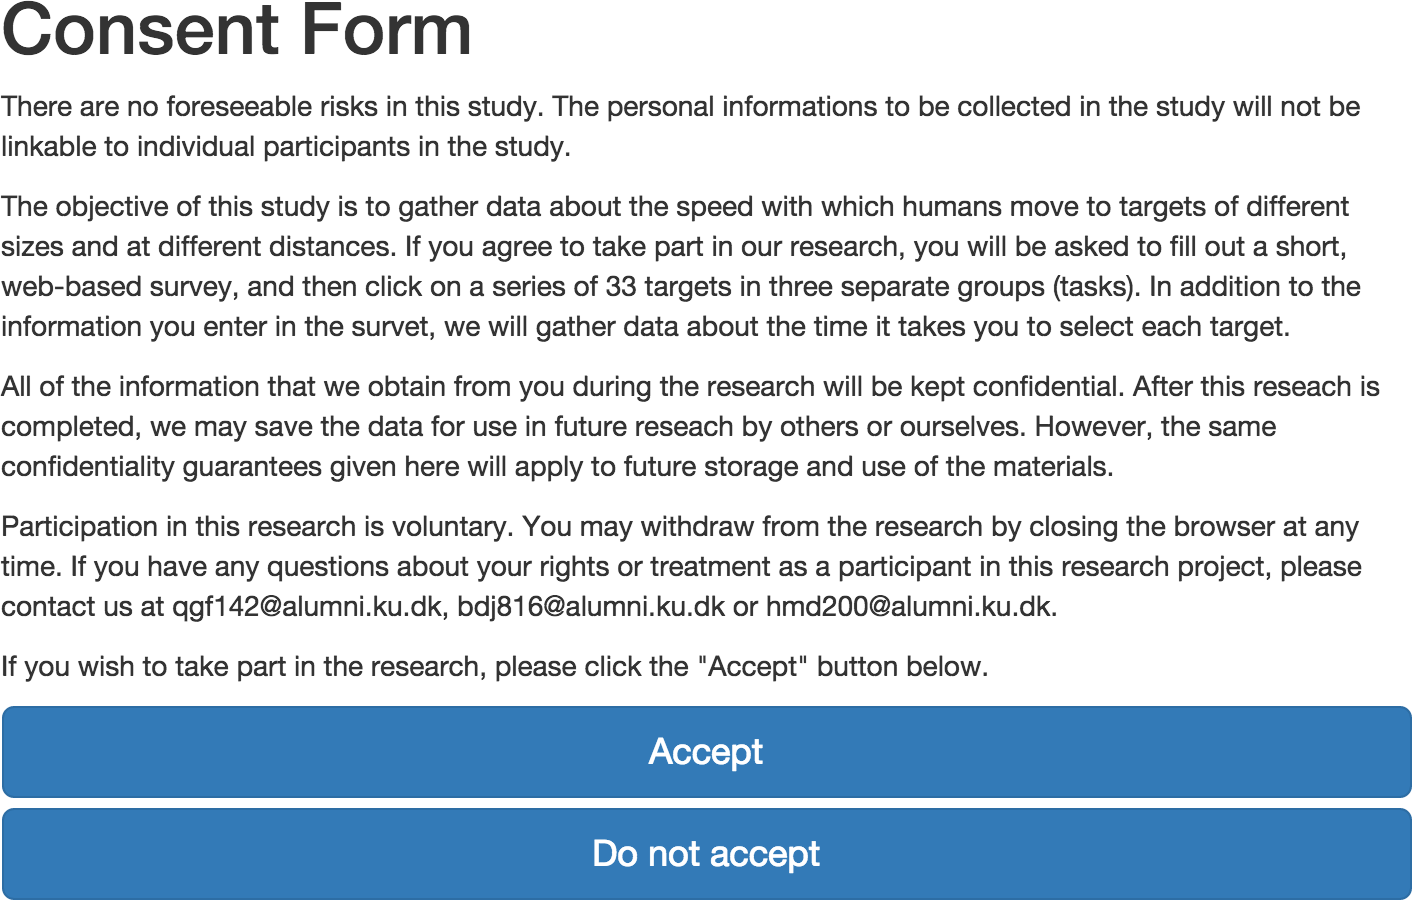
\includegraphics[width=\textwidth]{images/screenshots/ex_step_2_consent}
\captionof{figure}{Eksperiment - Trin 2 - Samtykke}
\label{fig:ex_step_2_consent}
\end{minipage}

\begin{minipage}{\textwidth}
\centering
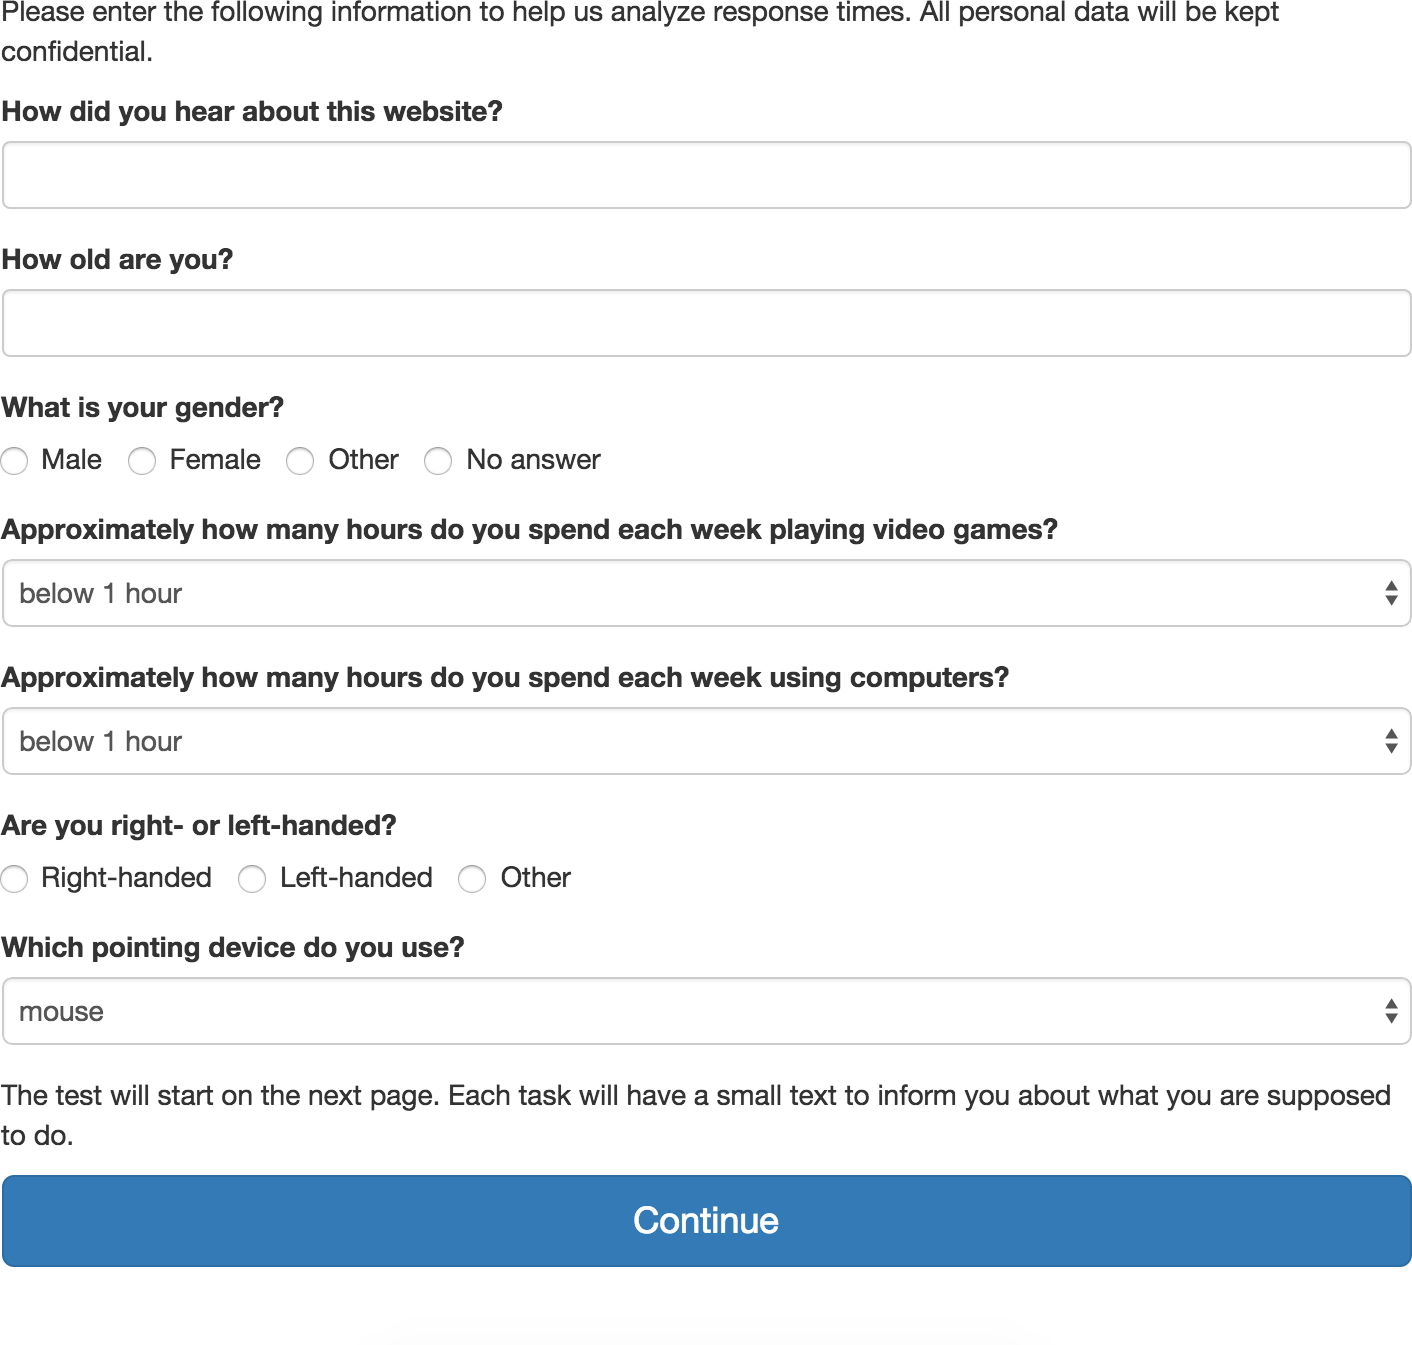
\includegraphics[width=\textwidth]{images/screenshots/ex_step_3_questions}
\captionof{figure}{Eksperiment - Trin 3 - Spørgsmål}
\label{fig:ex_step_3_questions}
\end{minipage}

\begin{minipage}{\textwidth}
\centering
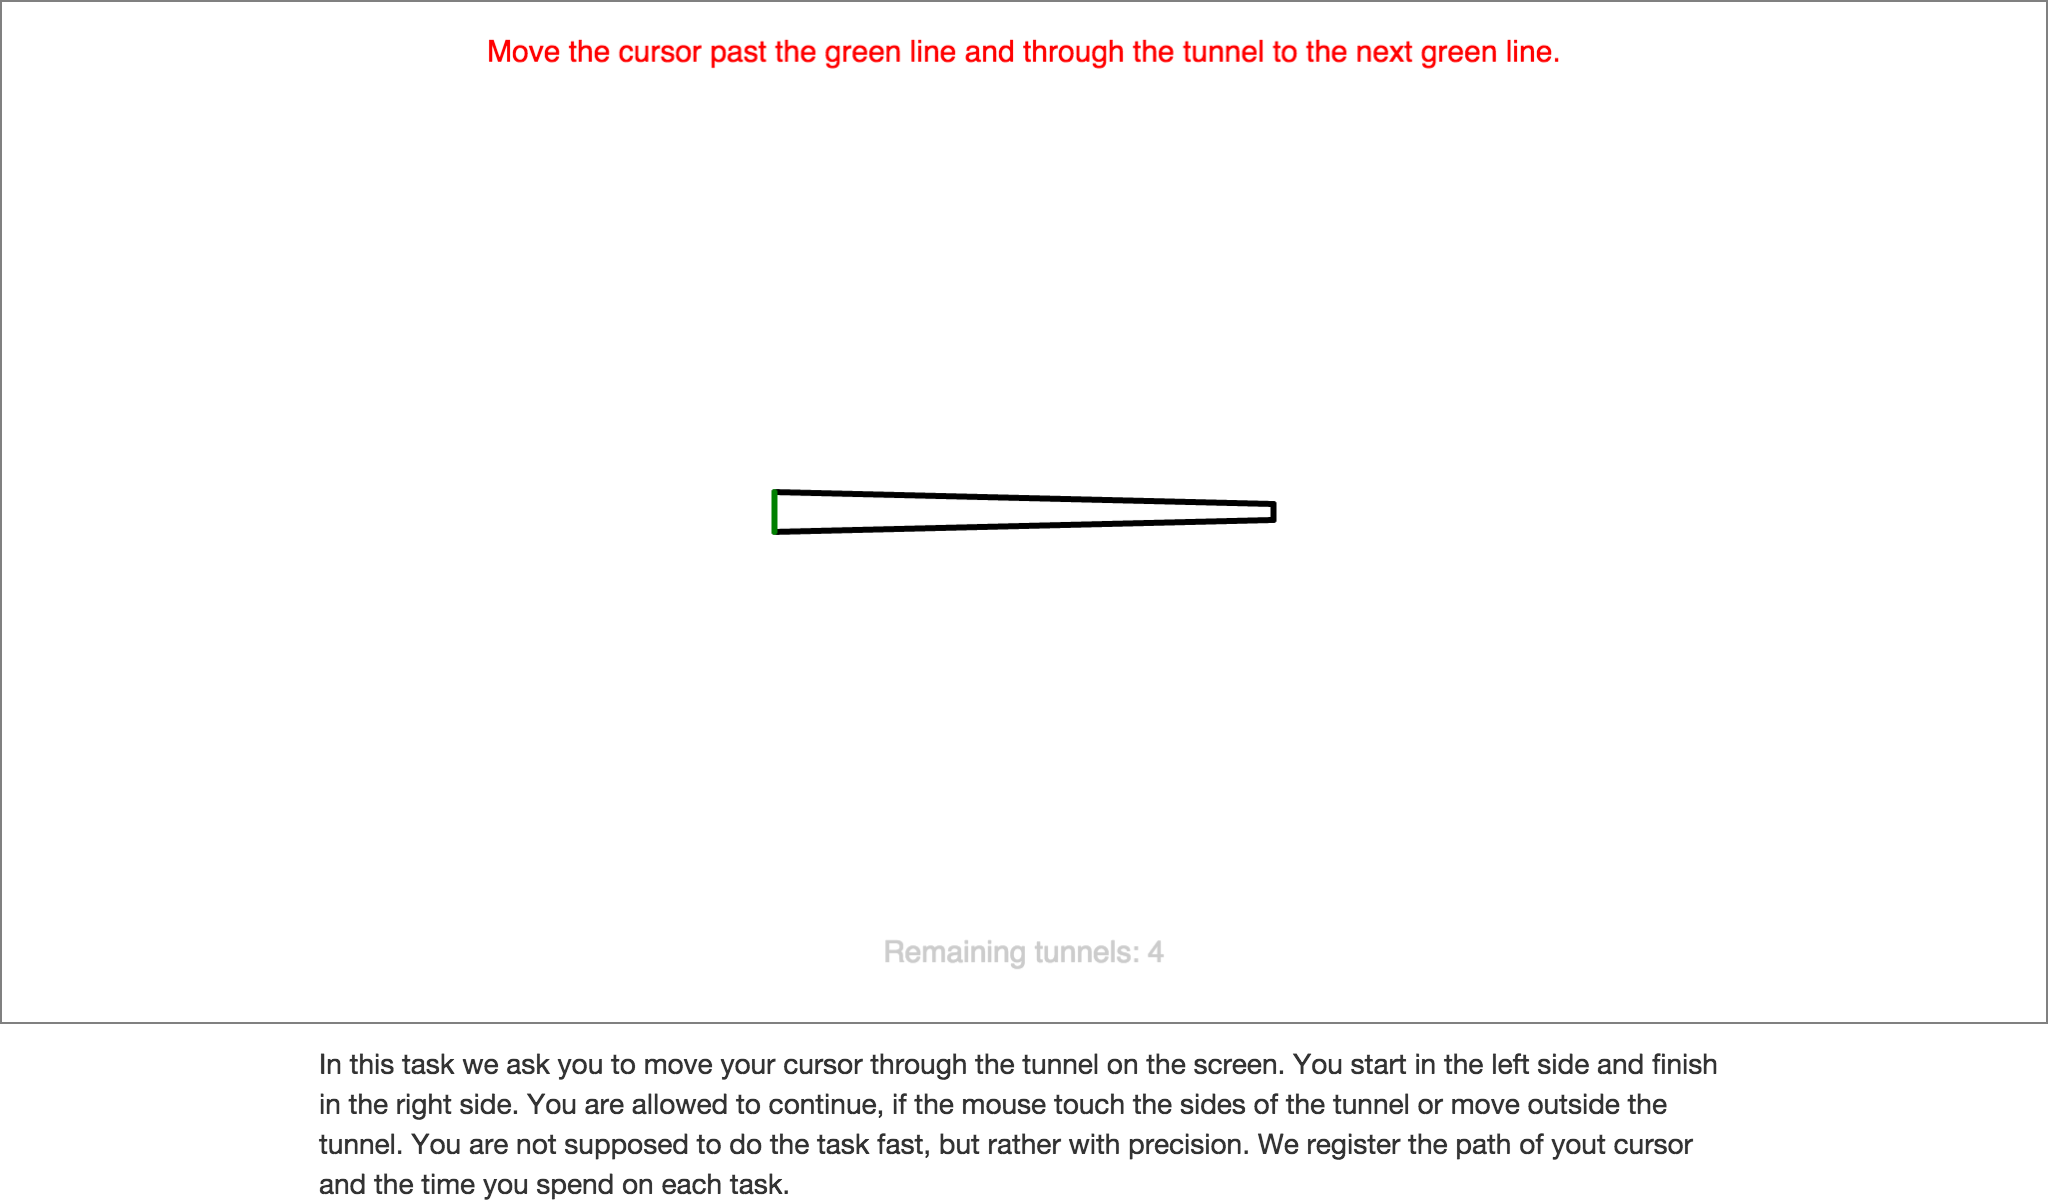
\includegraphics[width=\textwidth]{images/screenshots/ex_step_4_tunnel_1}
\captionof{figure}{Eksperiment - Trin 4 - Tunnel 1}
\label{fig:ex_step_4_tunnel_1}
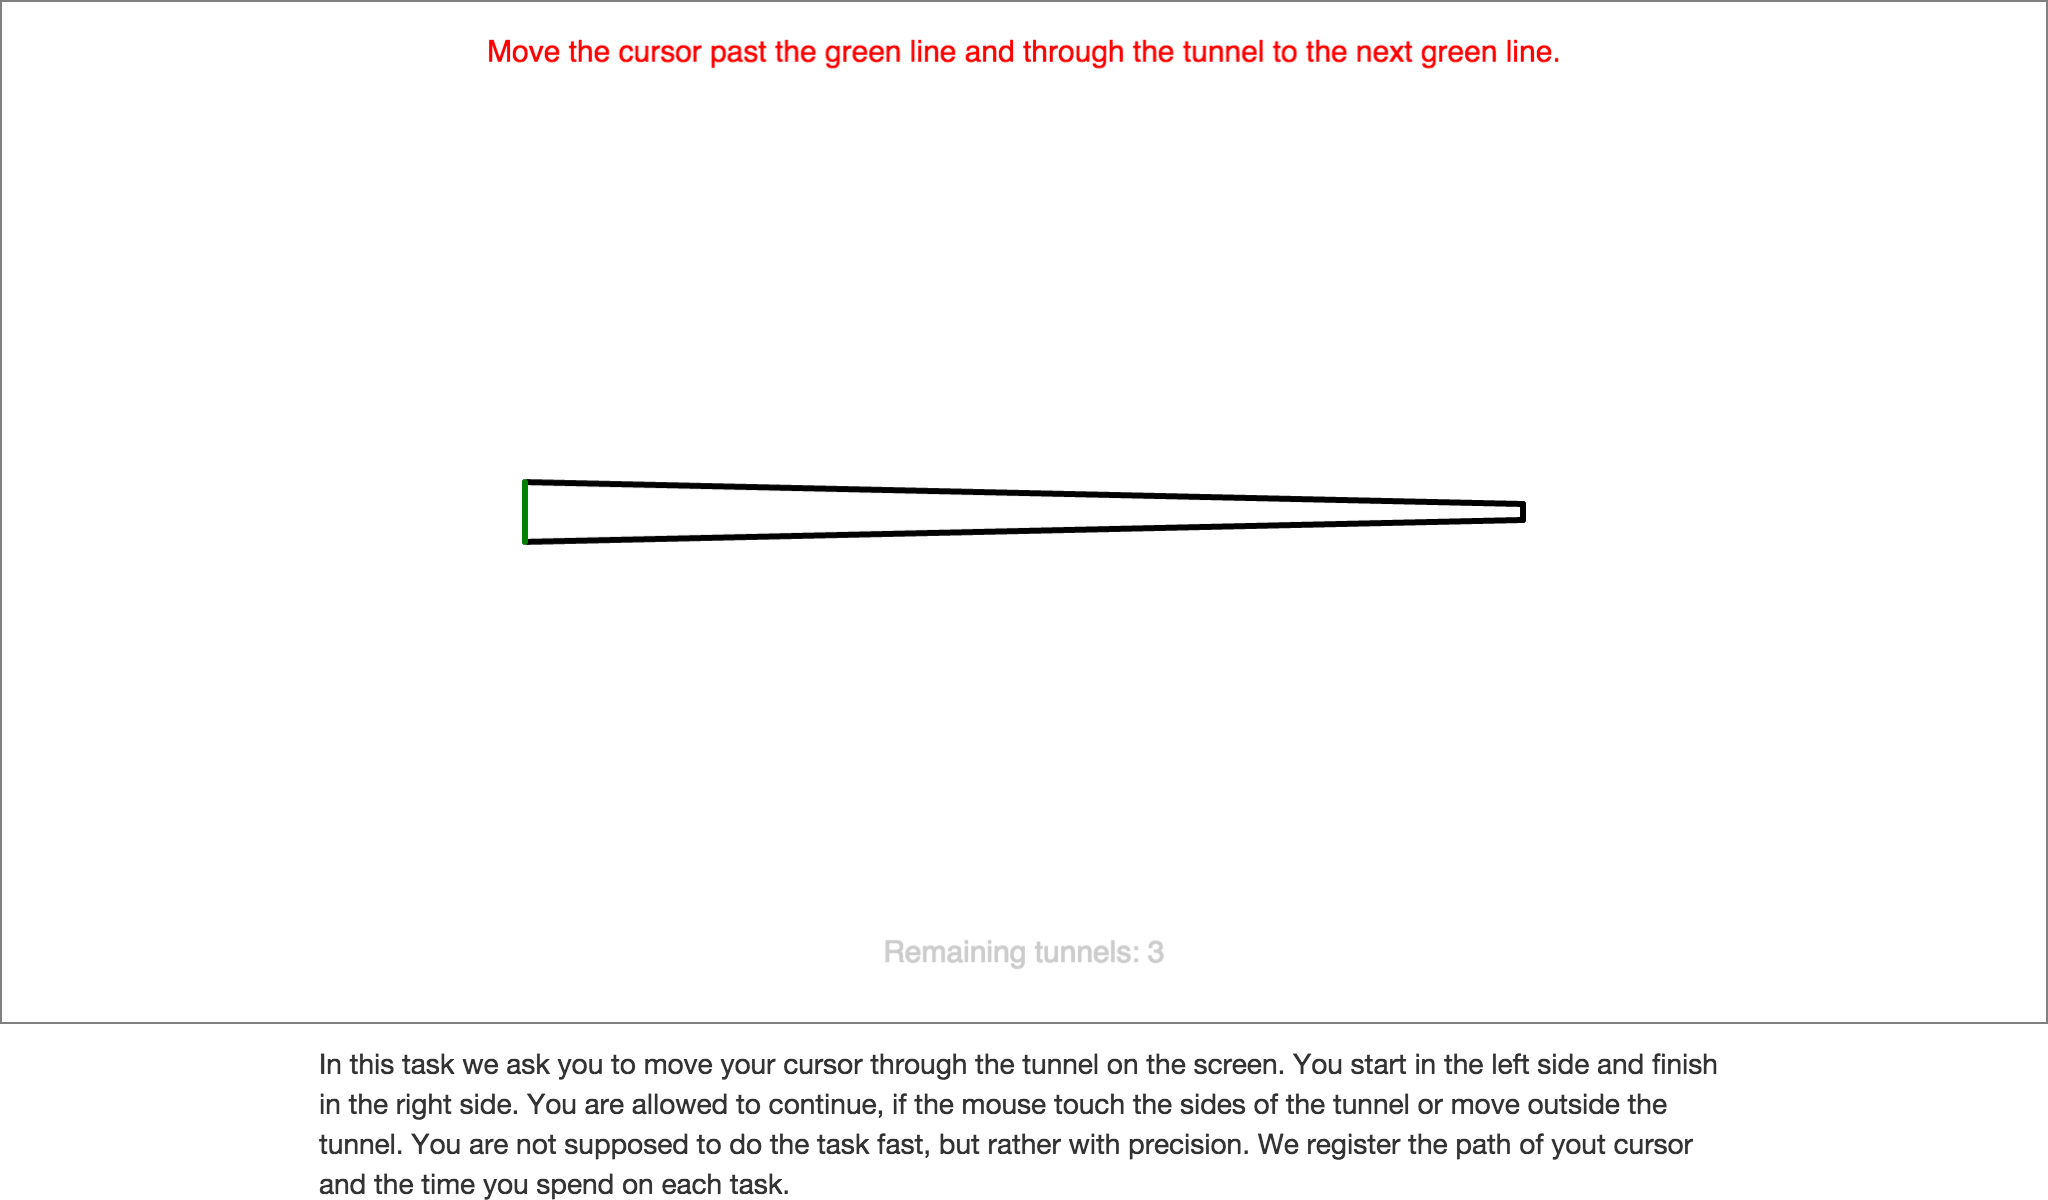
\includegraphics[width=\textwidth]{images/screenshots/ex_step_4_tunnel_2}
\captionof{figure}{Eksperiment - Trin 4 - Tunnel 2}
\label{fig:ex_step_4_tunnel_2}
\end{minipage}

\begin{minipage}{\textwidth}
\centering
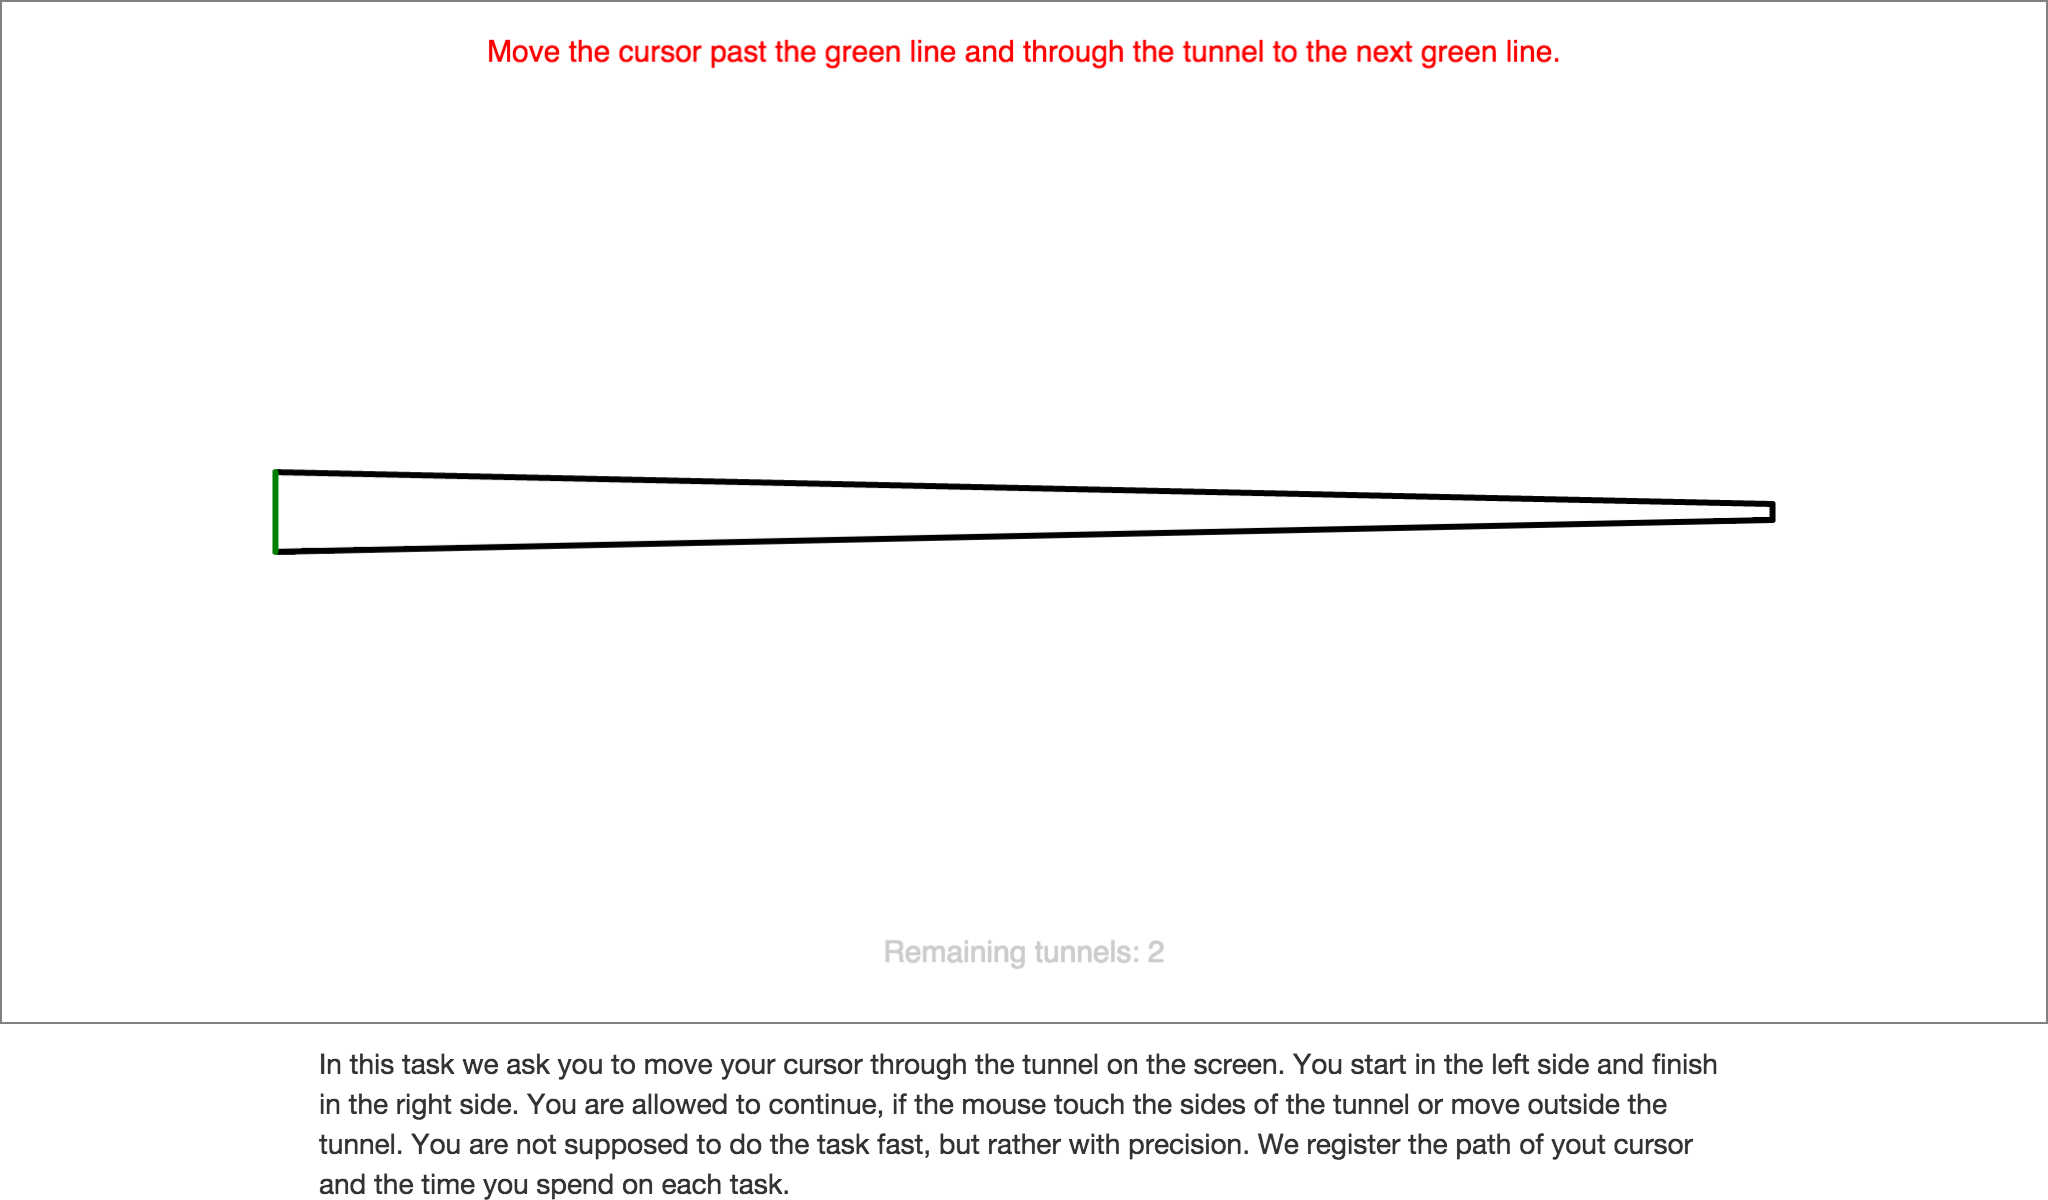
\includegraphics[width=\textwidth]{images/screenshots/ex_step_4_tunnel_3}
\captionof{figure}{Eksperiment - Trin 4 - Tunnel 3}
\label{fig:ex_step_4_tunnel_3}
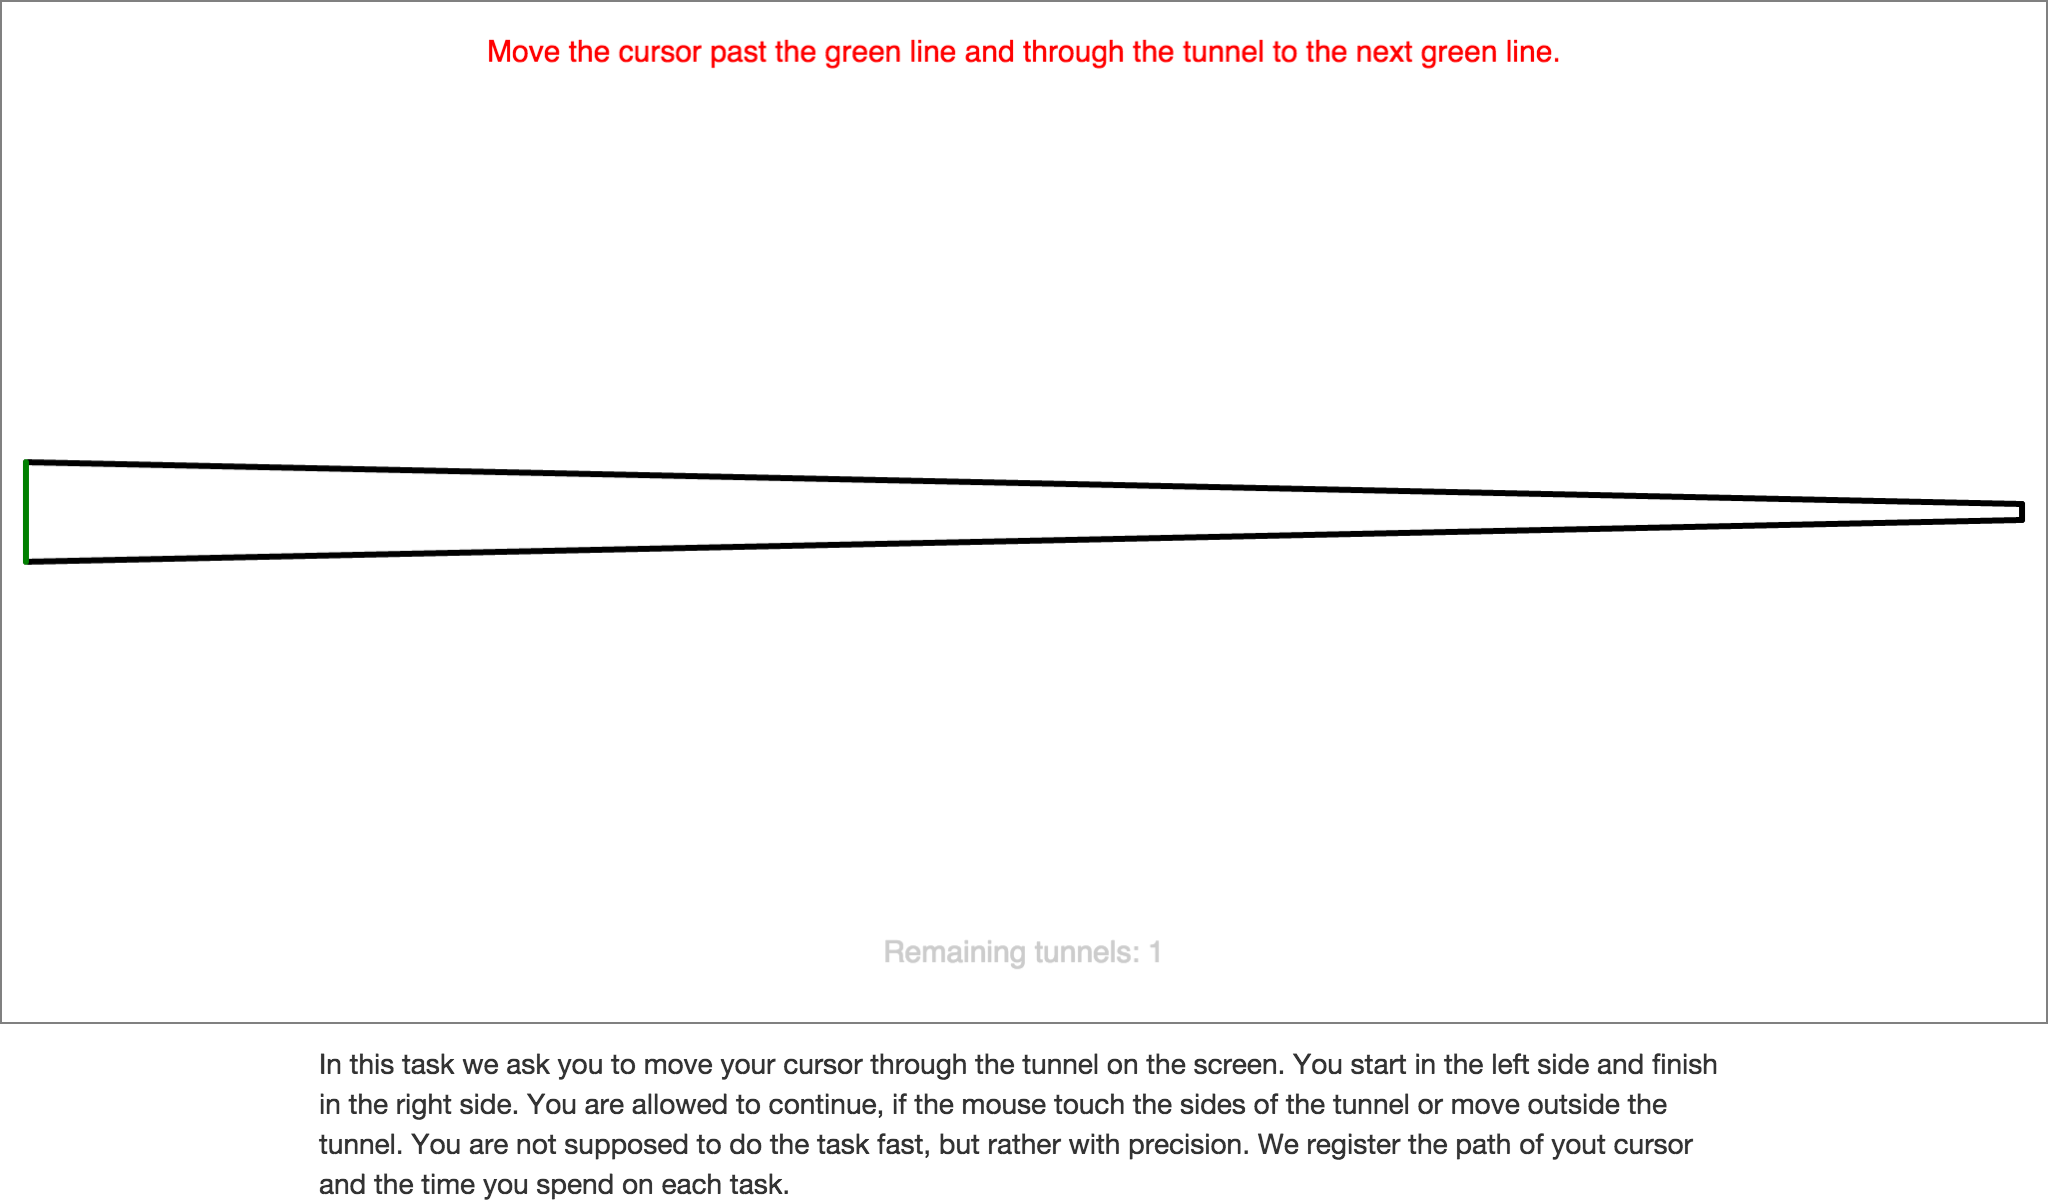
\includegraphics[width=\textwidth]{images/screenshots/ex_step_4_tunnel_4}
\captionof{figure}{Eksperiment - Trin 4 - Tunnel 4}
\label{fig:ex_step_4_tunnel_3}
\end{minipage}

\begin{minipage}{\textwidth}
\centering
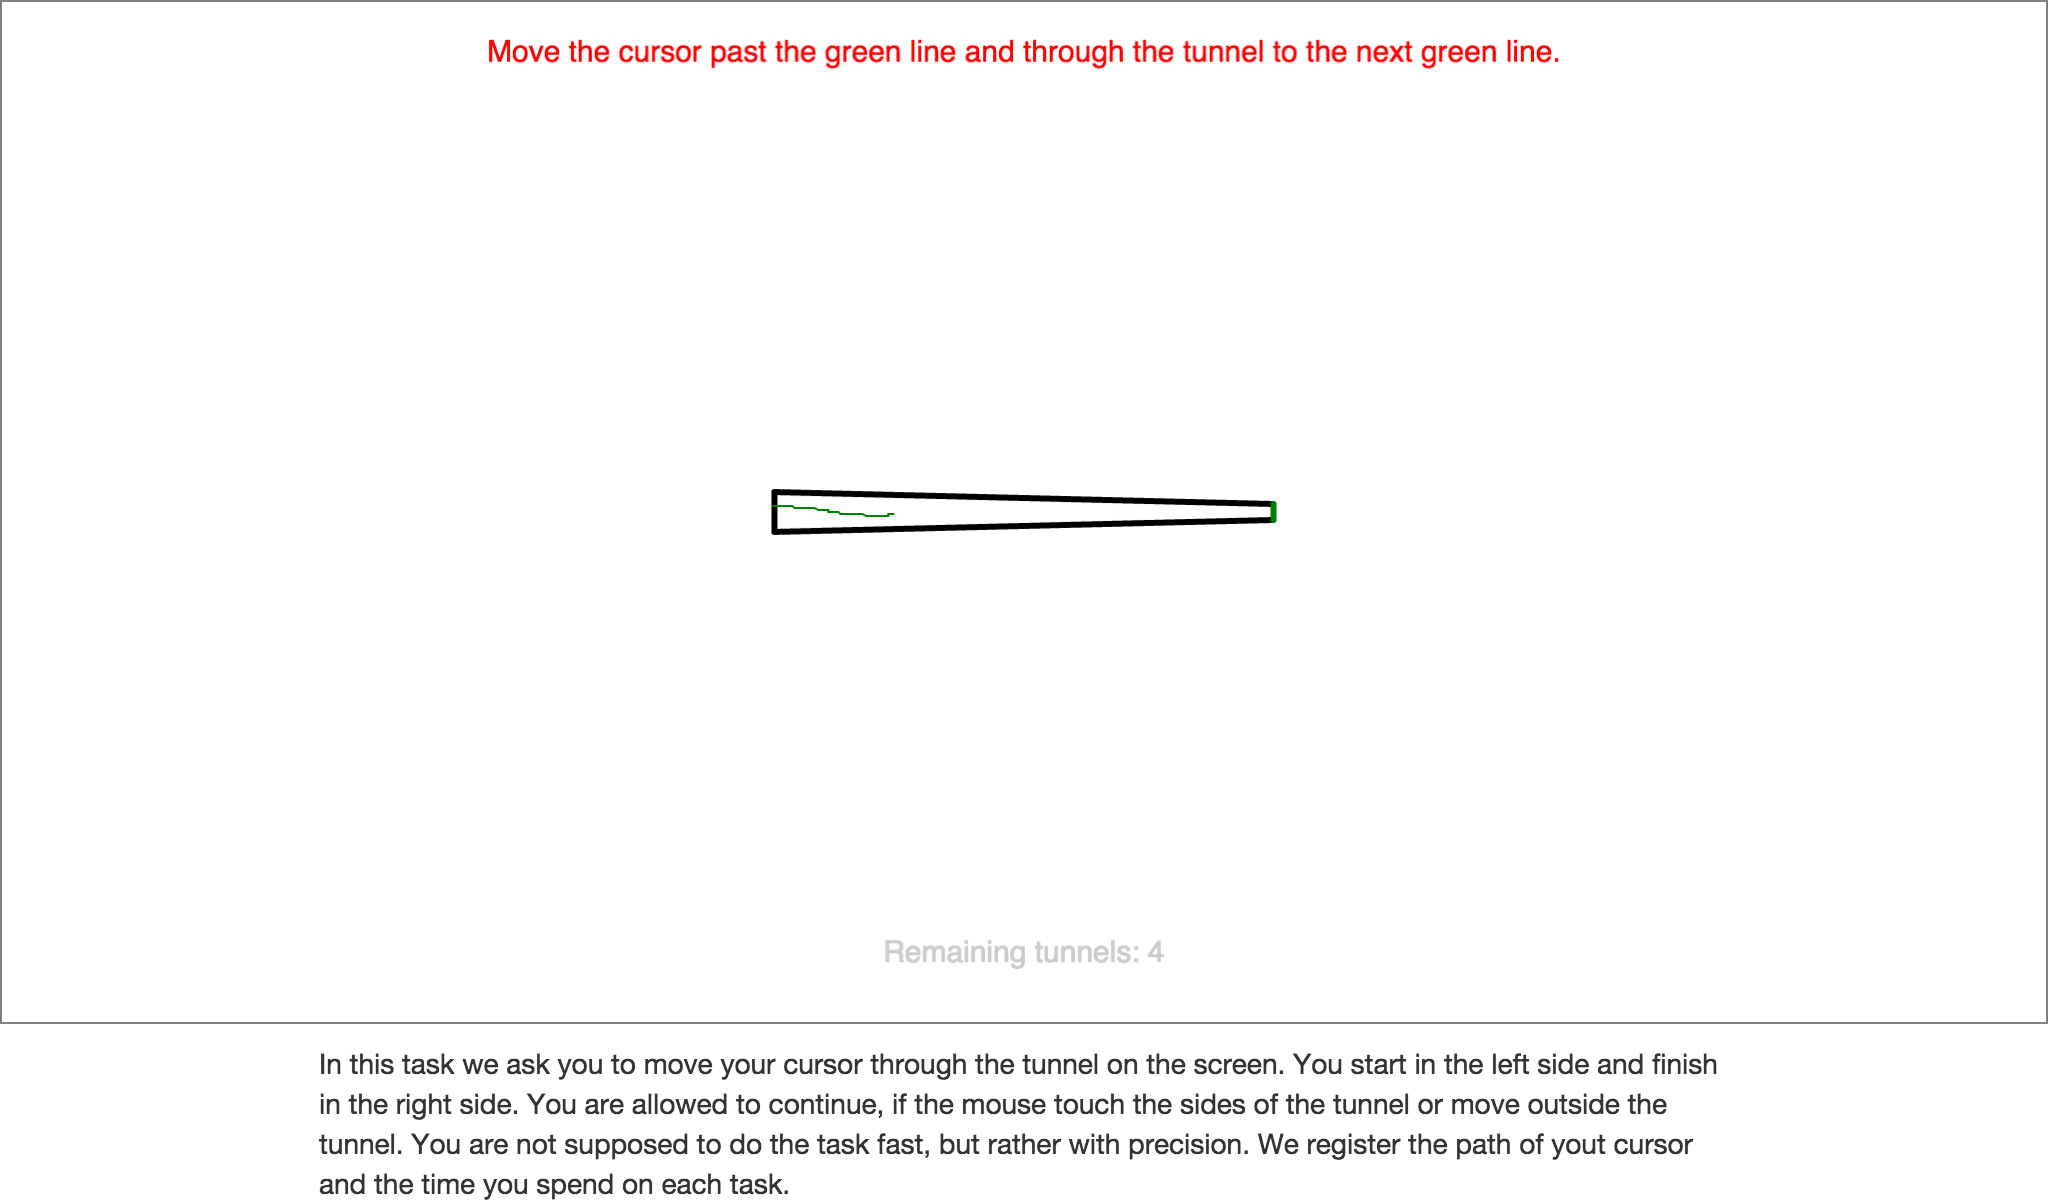
\includegraphics[width=\textwidth]{images/screenshots/ex_step_4_tunnel_path}
\captionof{figure}{Eksperiment - Trin 4 - Tunnelbane}
\label{fig:ex_step_4_tunnel_path}
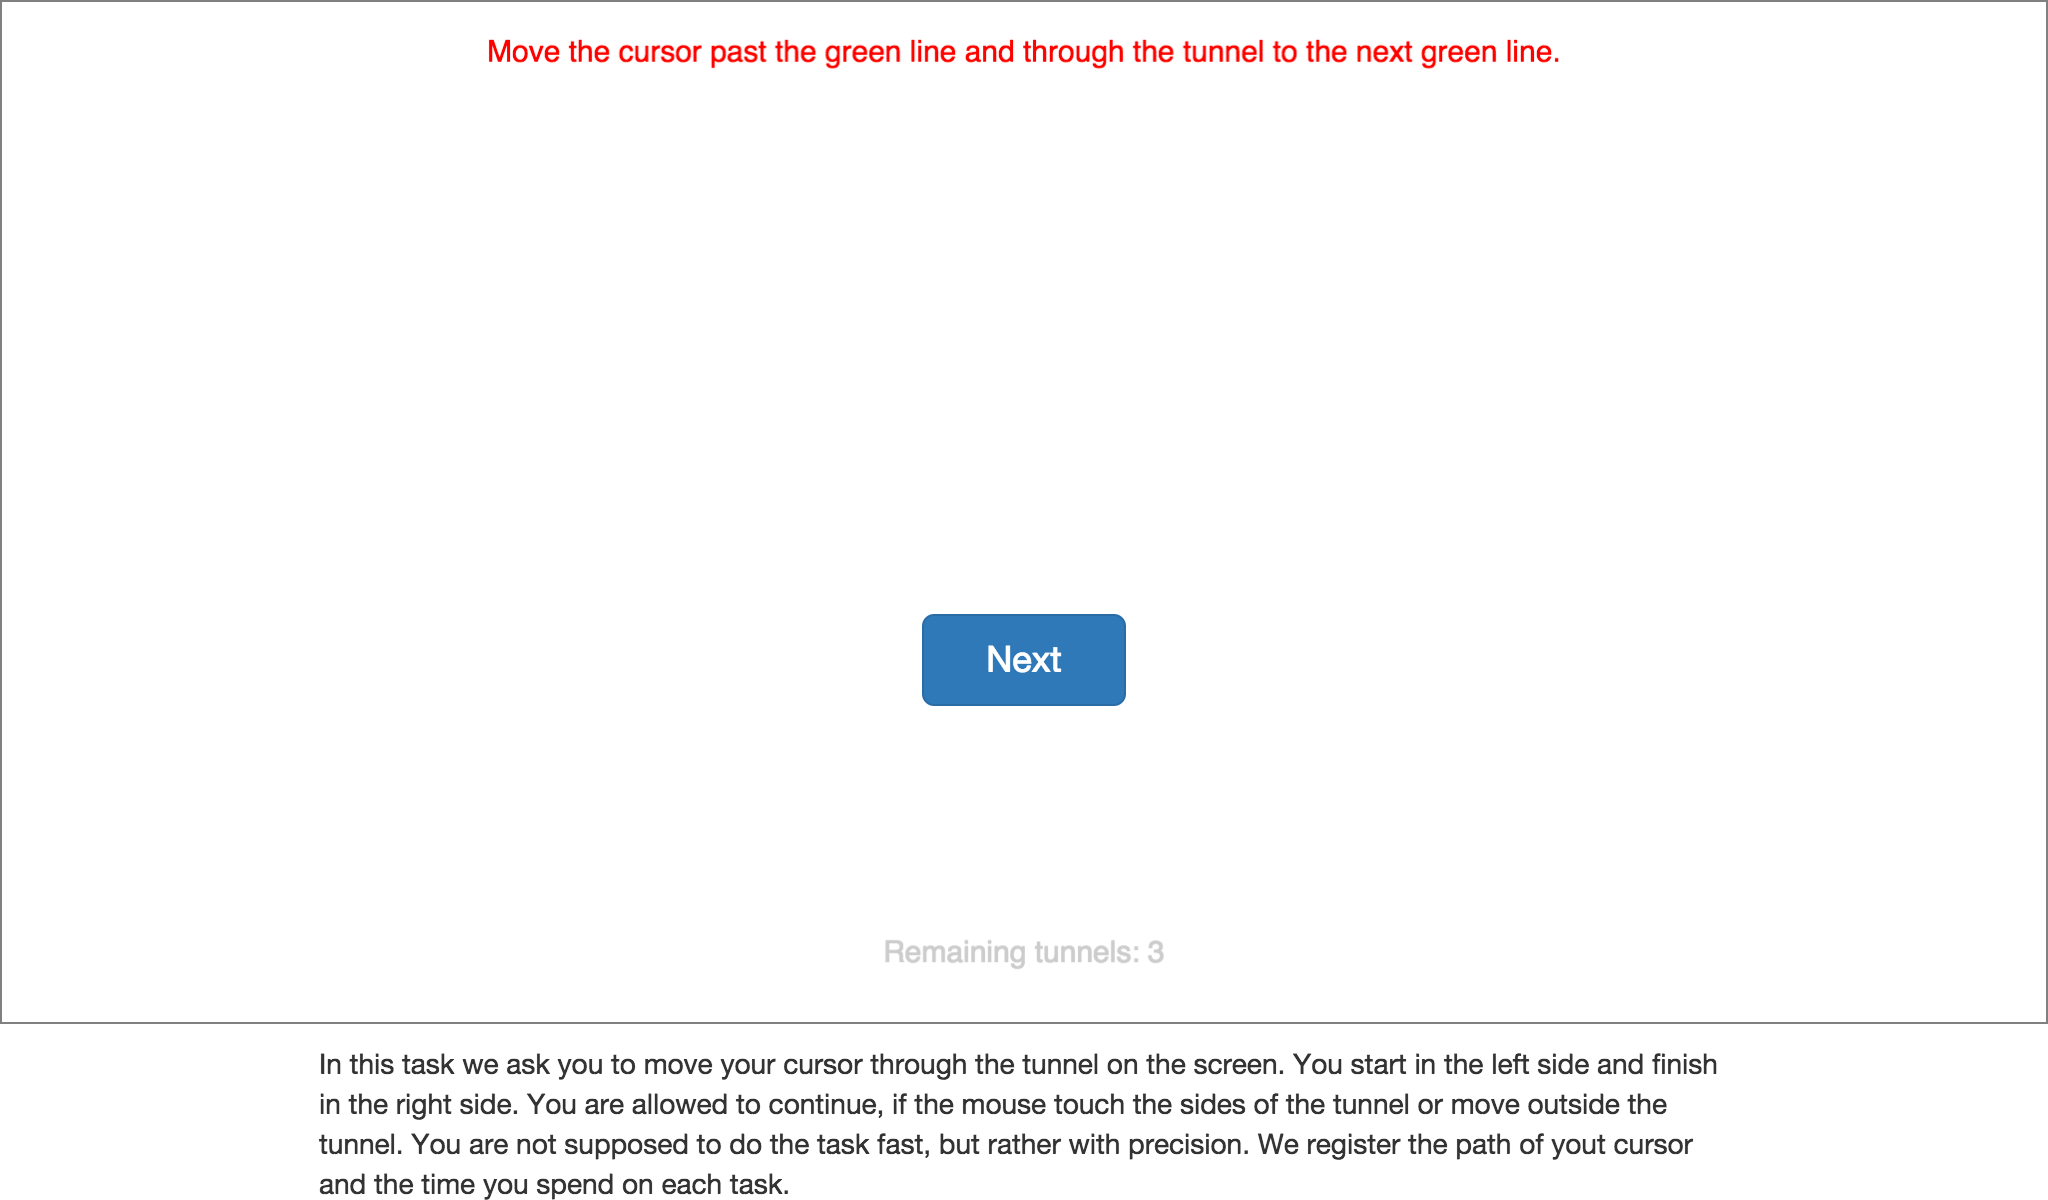
\includegraphics[width=\textwidth]{images/screenshots/ex_step_4_tunnel_next}
\captionof{figure}{Eksperiment - Trin 4 - Næste tunnel}
\label{fig:ex_step_4_tunnel_next}
\end{minipage}

\begin{minipage}{\textwidth}
\centering
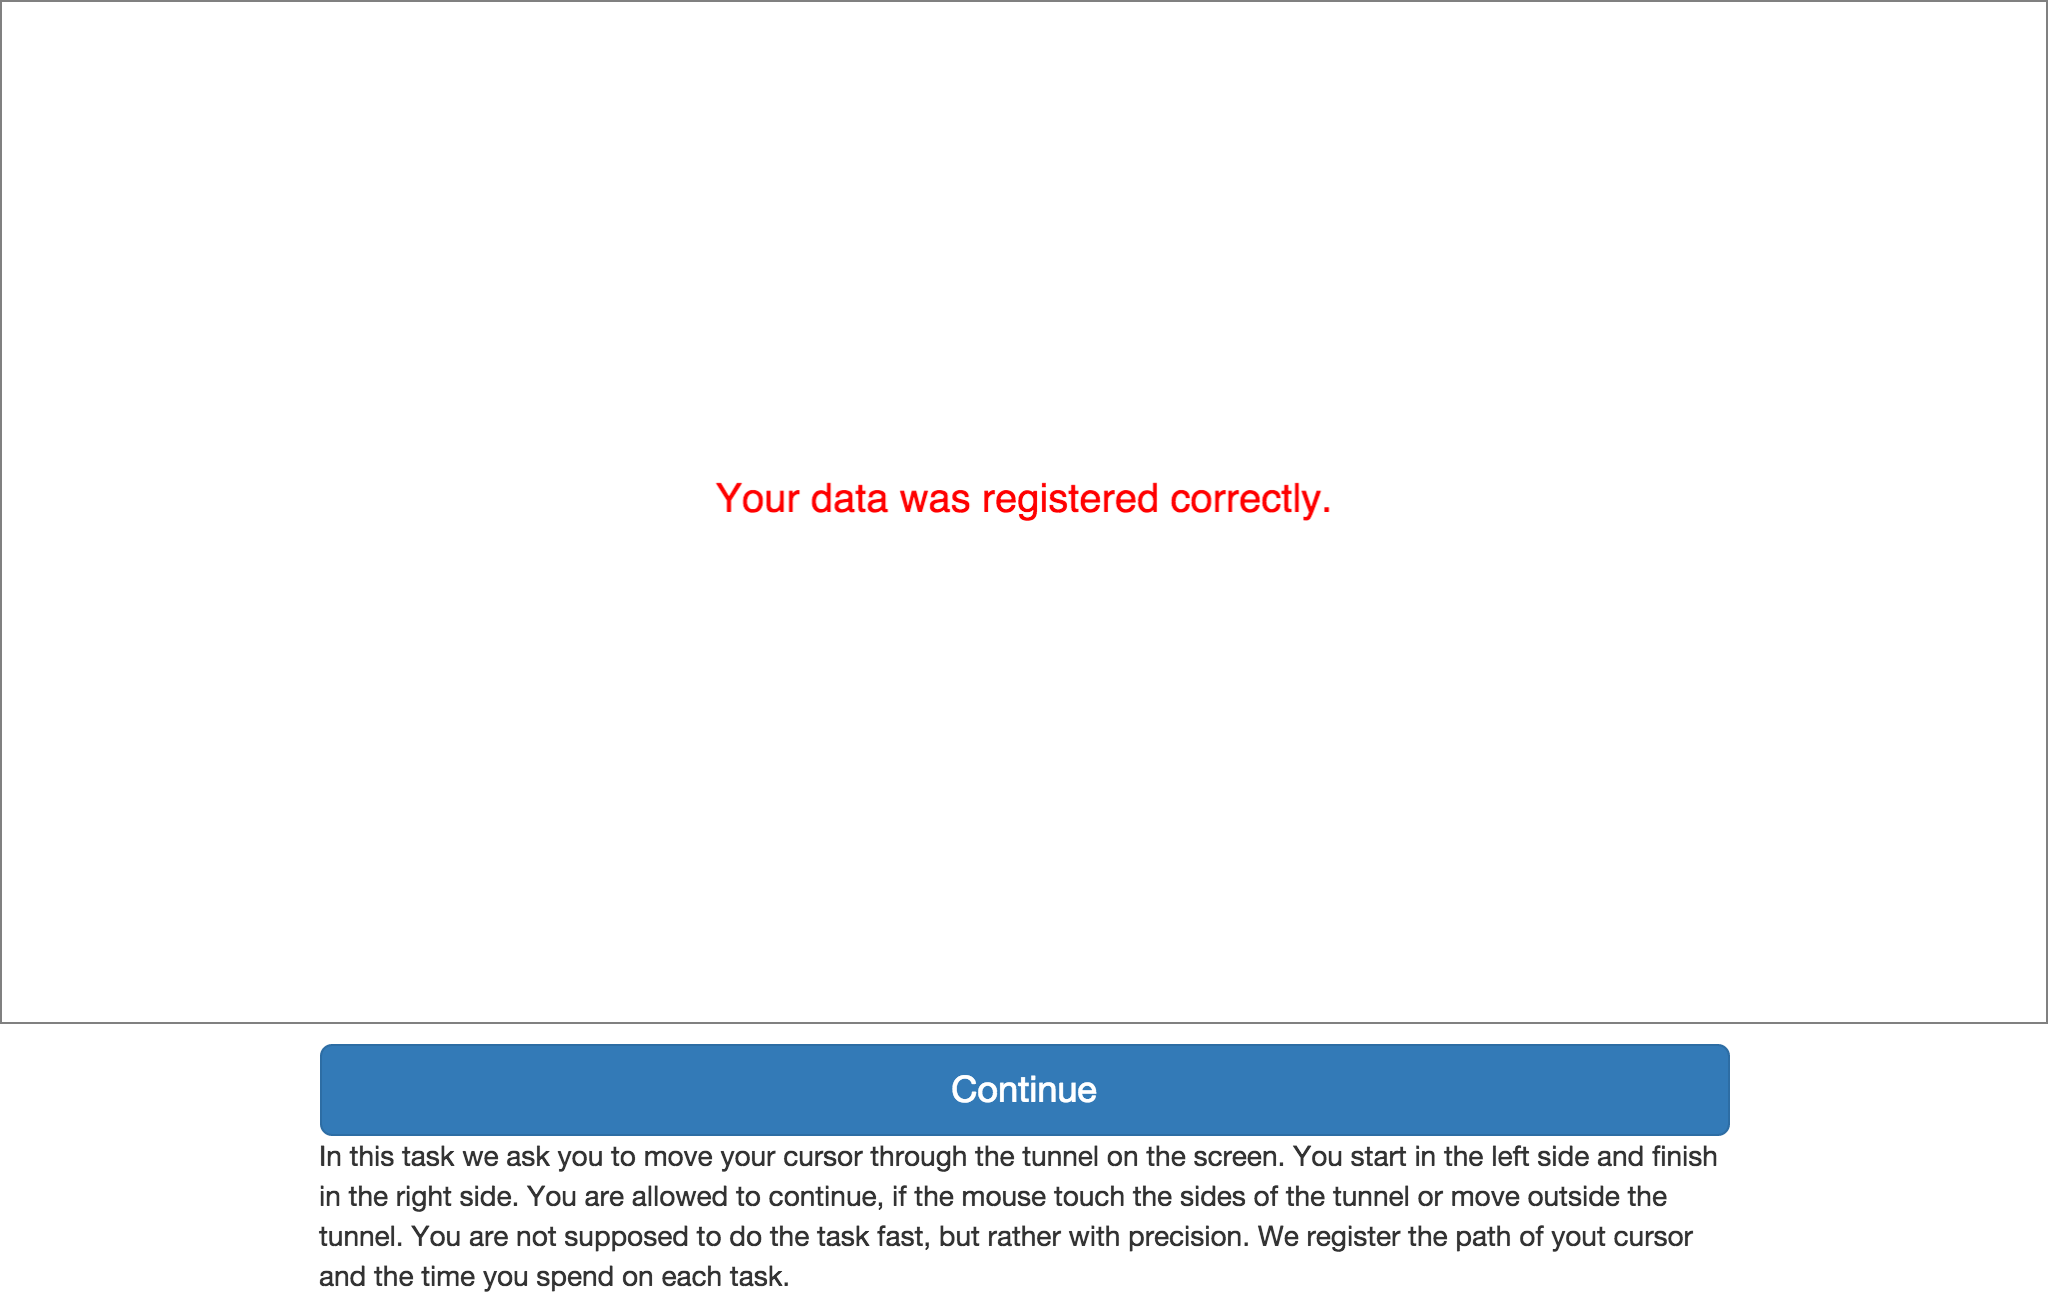
\includegraphics[width=\textwidth]{images/screenshots/ex_step_4_tunnel_done}
\captionof{figure}{Eksperiment - Trin 4 - Fortsæt}
\label{fig:ex_step_4_tunnel_done}
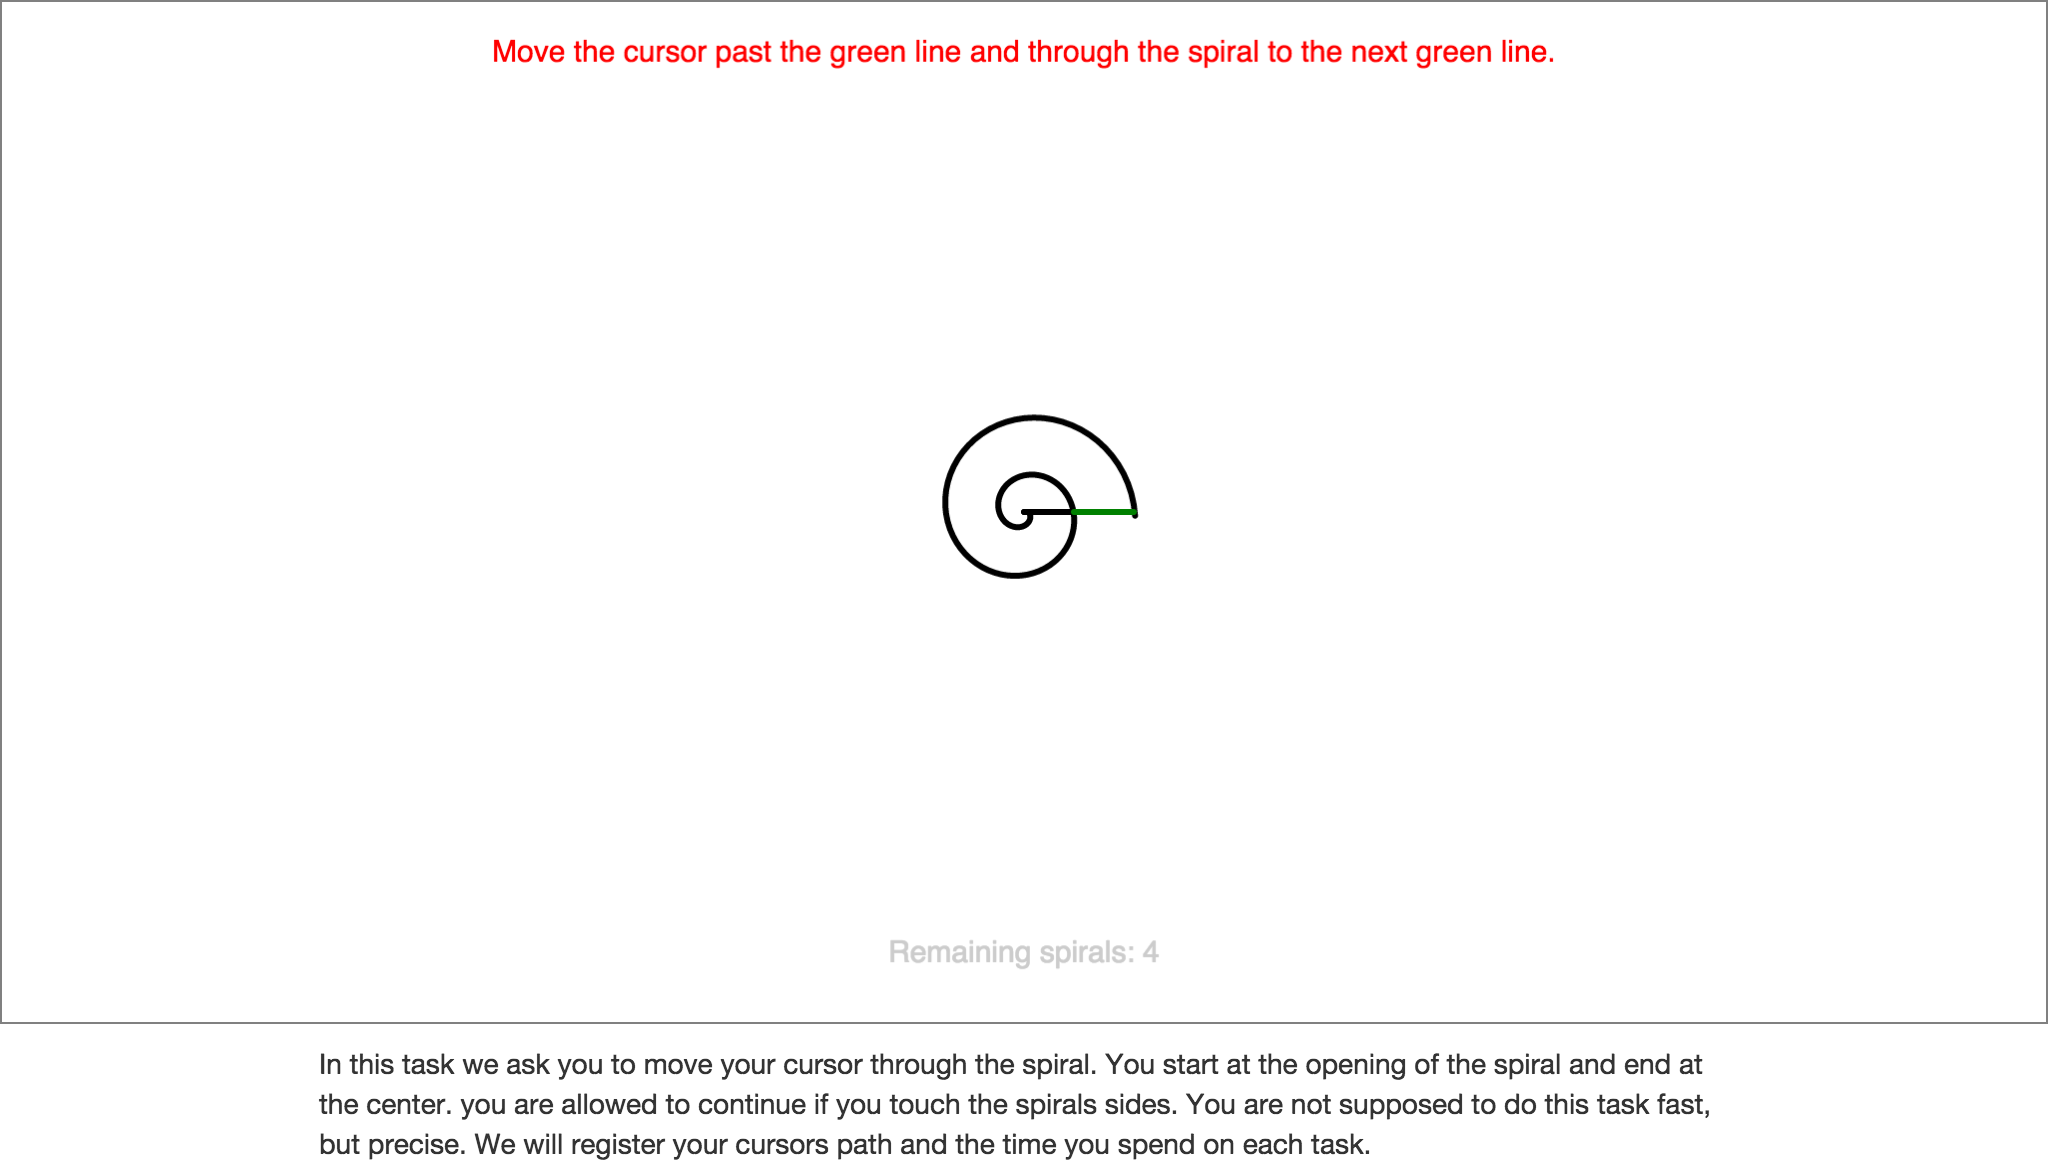
\includegraphics[width=\textwidth]{images/screenshots/ex_step_5_spiral_1}
\captionof{figure}{Eksperiment - Trin 5 - Spiral 1}
\label{fig:ex_step_5_spiral_1}
\end{minipage}

\begin{minipage}{\textwidth}
\centering
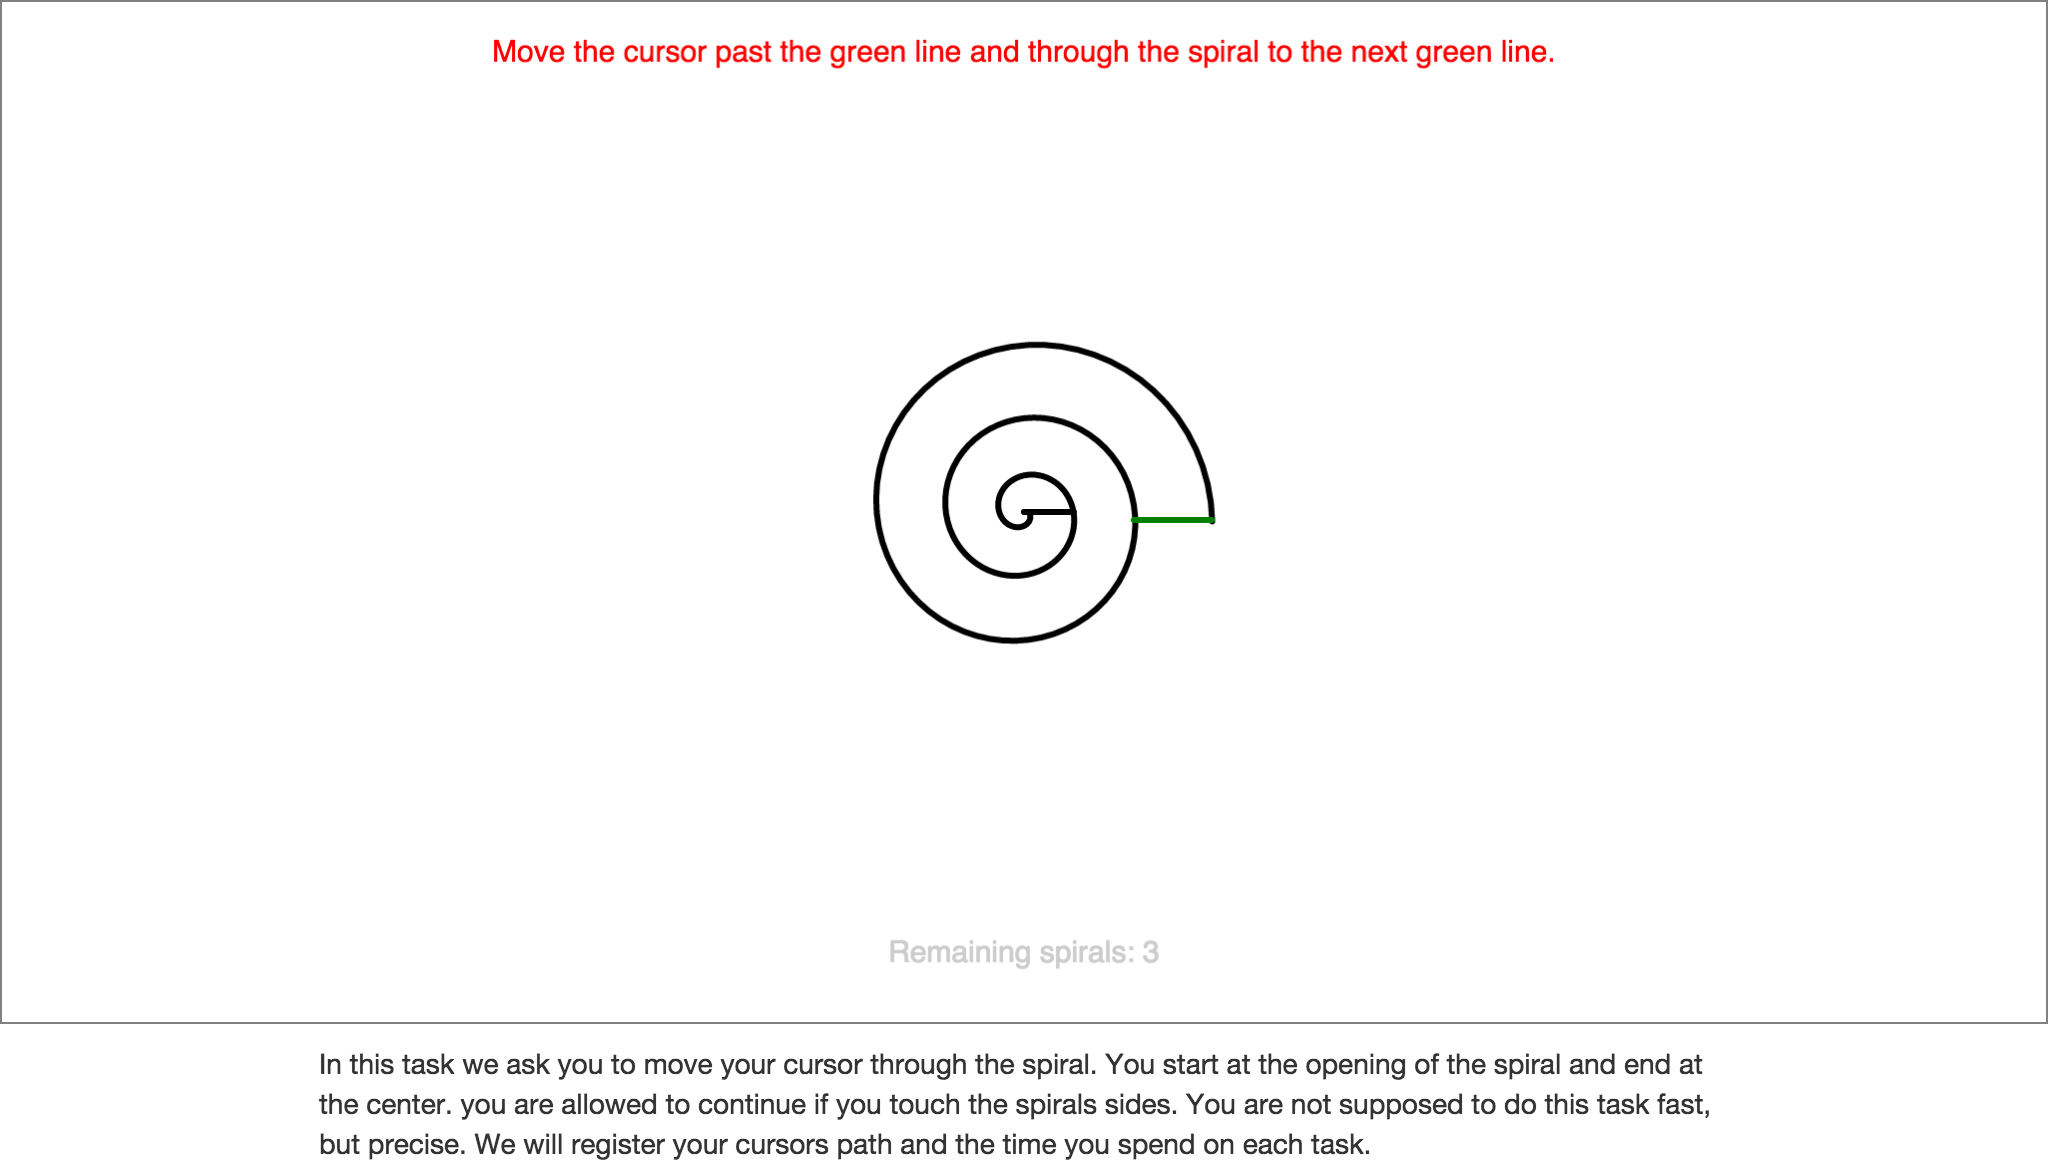
\includegraphics[width=\textwidth]{images/screenshots/ex_step_5_spiral_2}
\captionof{figure}{Eksperiment - Trin 5 - Spiral 2}
\label{fig:ex_step_5_spiral_2}
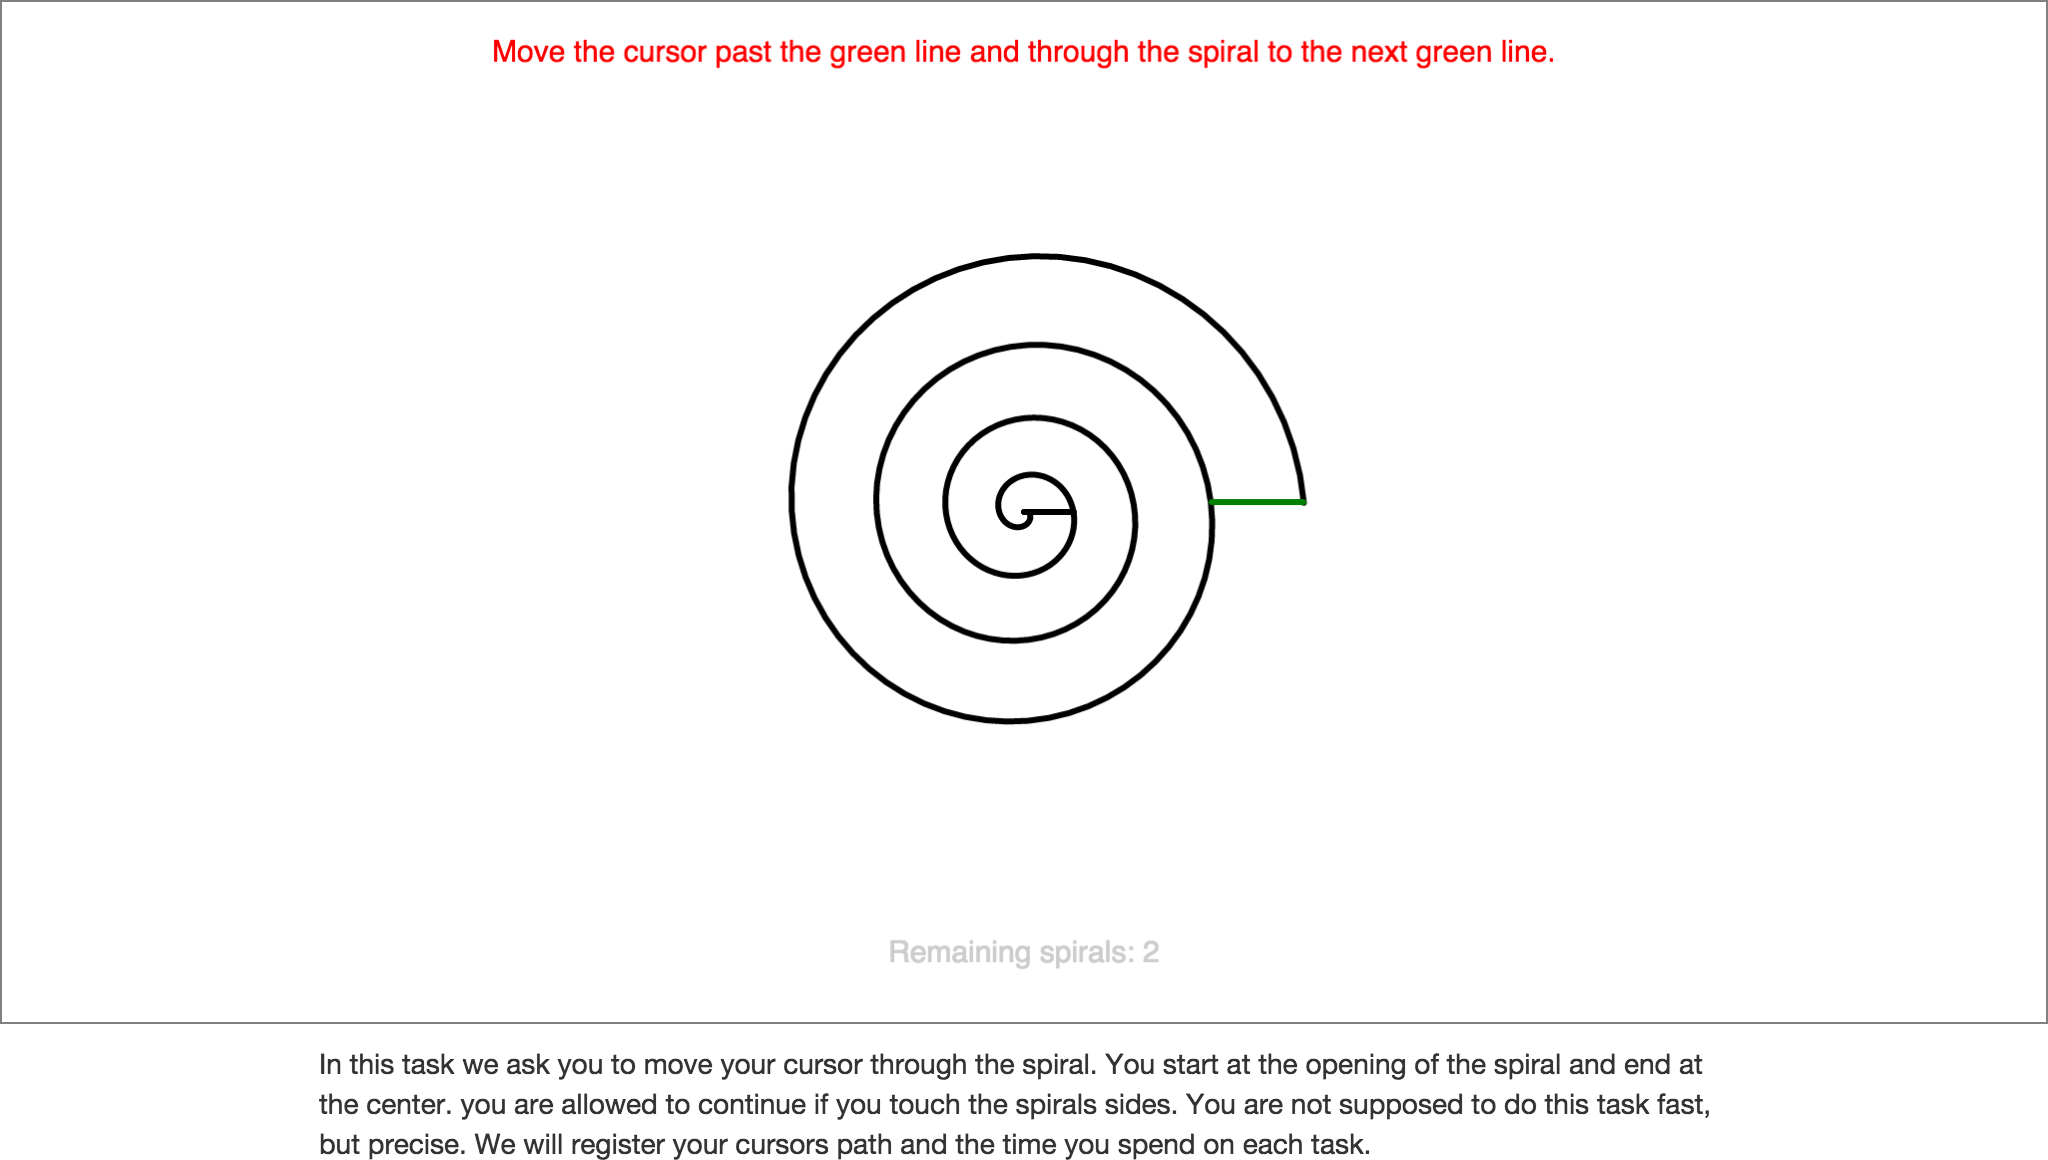
\includegraphics[width=\textwidth]{images/screenshots/ex_step_5_spiral_3}
\captionof{figure}{Eksperiment - Trin 5 - Spiral 3}
\label{fig:ex_step_5_spiral_3}
\end{minipage}

\begin{minipage}{\textwidth}
\centering
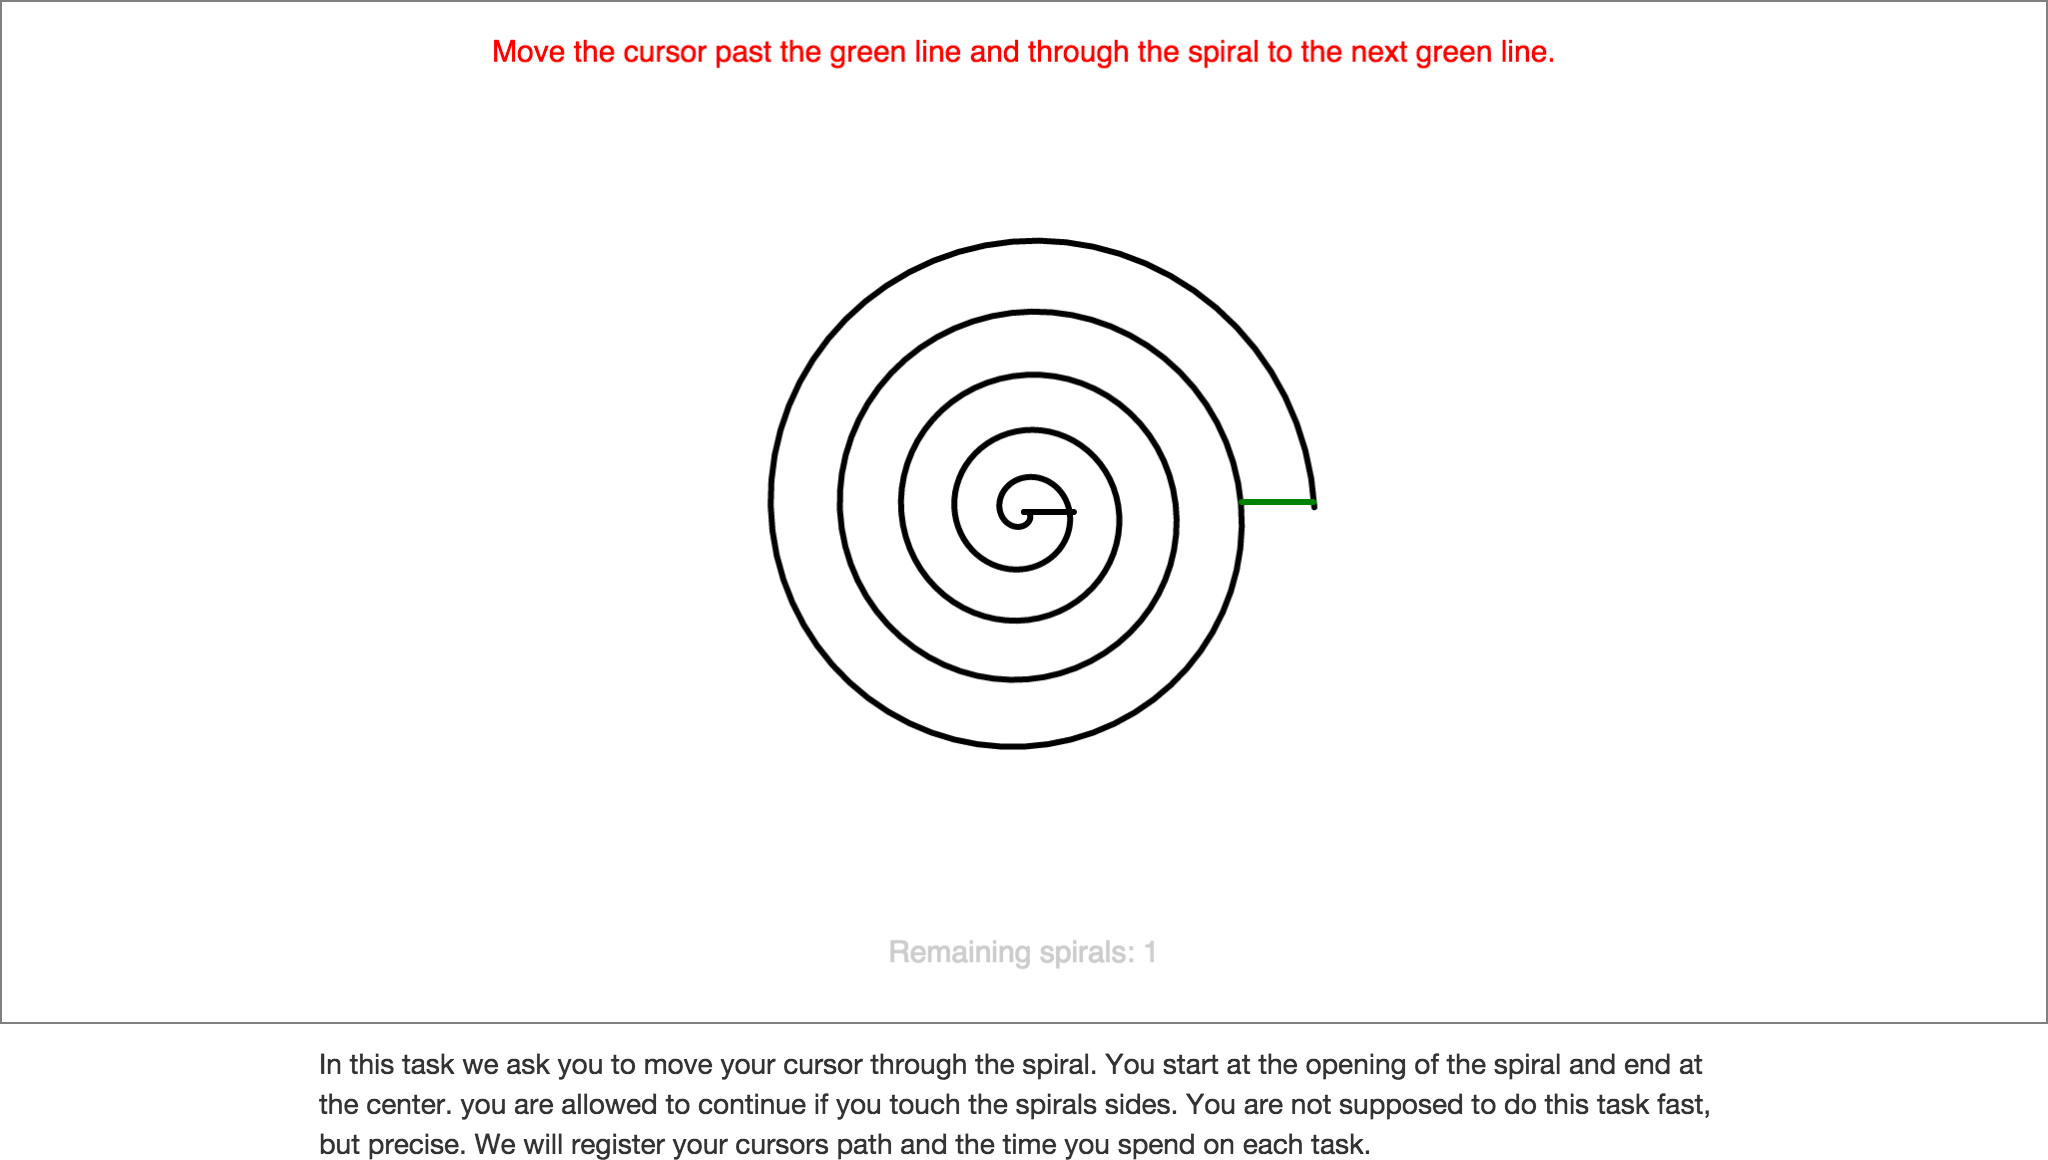
\includegraphics[width=\textwidth]{images/screenshots/ex_step_5_spiral_4}
\captionof{figure}{Eksperiment - Trin 5 - Spiral 4}
\label{fig:ex_step_5_spiral_4}
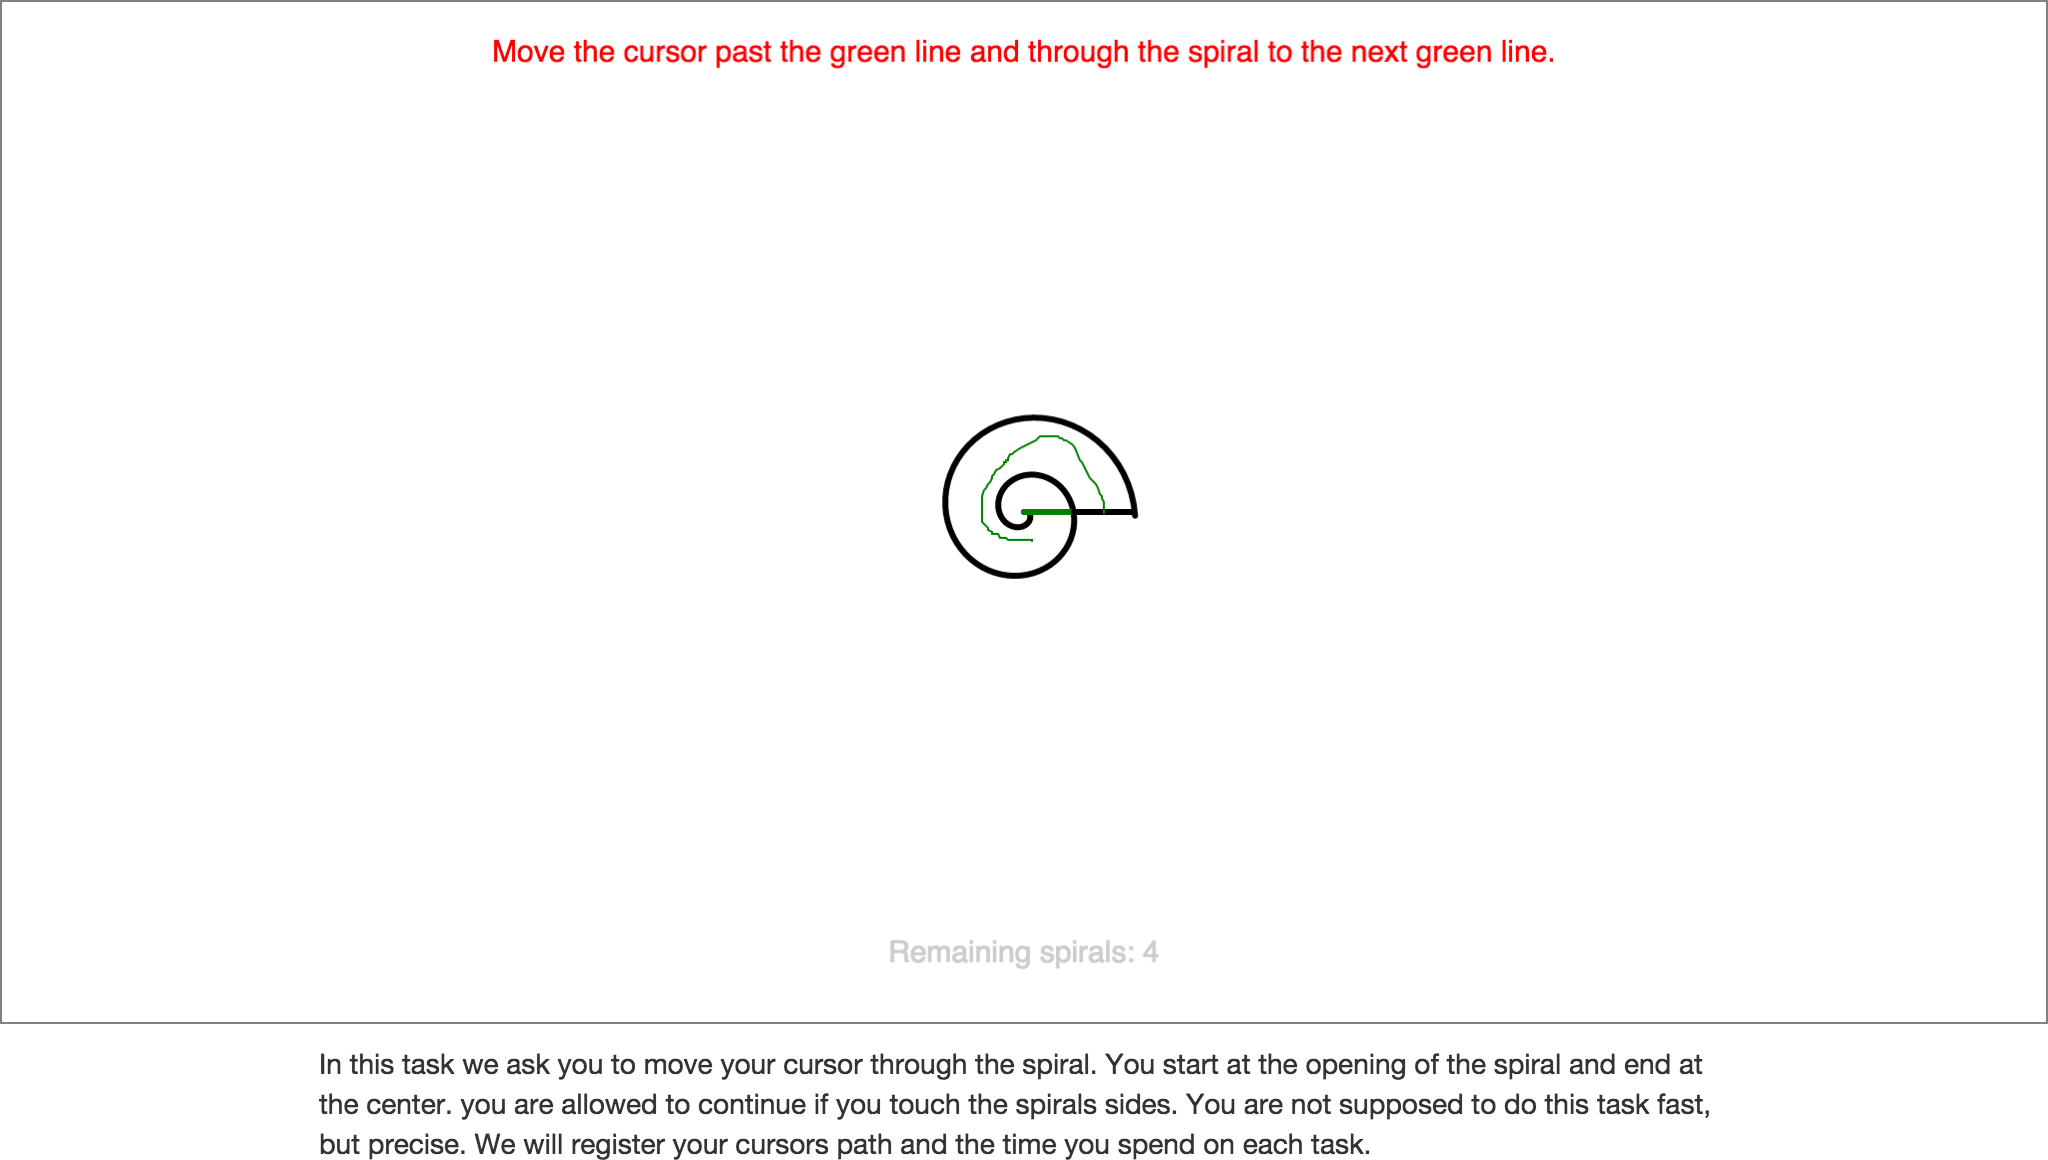
\includegraphics[width=\textwidth]{images/screenshots/ex_step_5_spiral_path}
\captionof{figure}{Eksperiment - Trin 5 - Spiralbane}
\label{fig:ex_step_5_spiral_path}
\end{minipage}

\begin{minipage}{\textwidth}
\centering
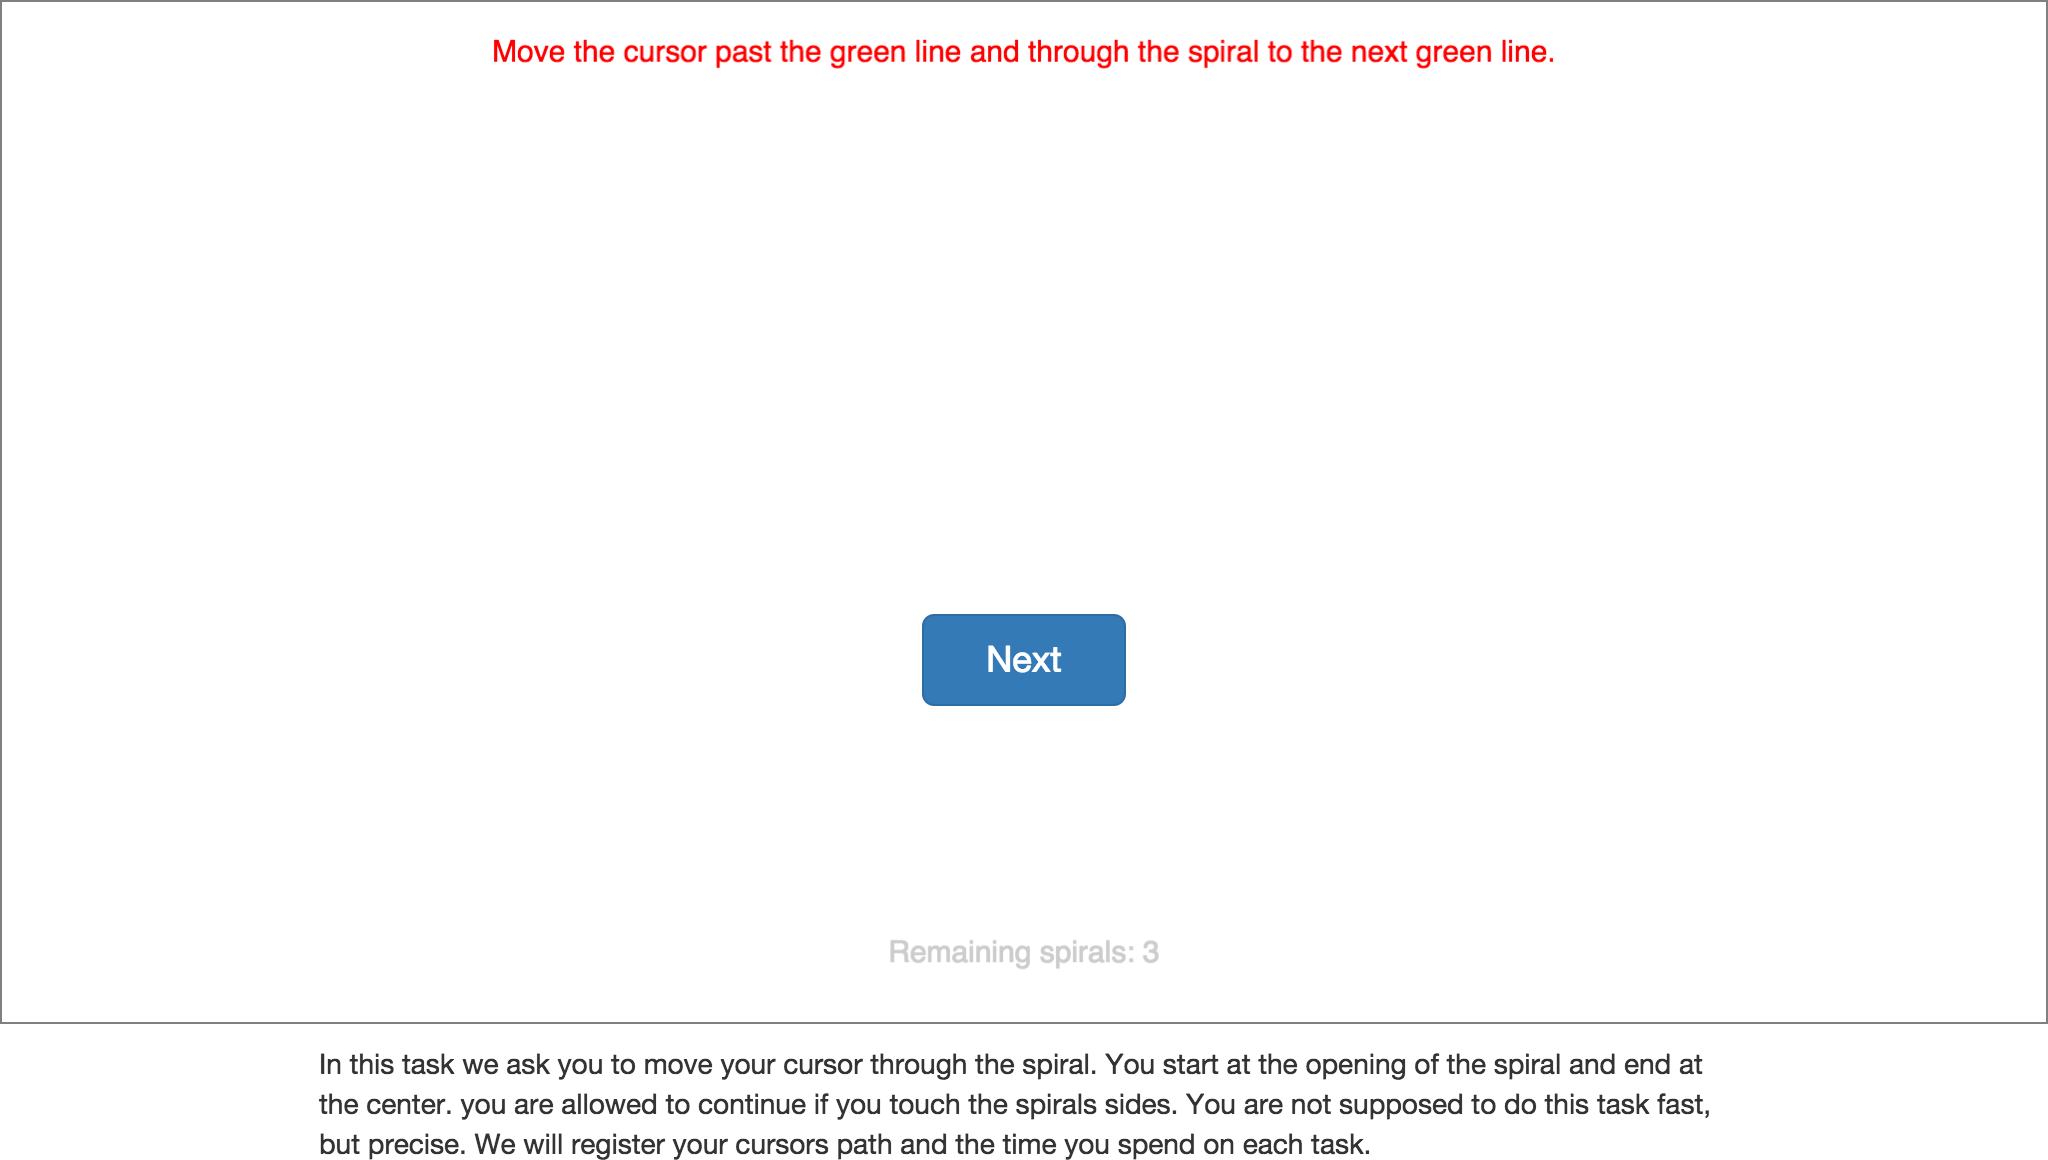
\includegraphics[width=\textwidth]{images/screenshots/ex_step_5_spiral_next}
\captionof{figure}{Eksperiment - Trin 5 - Næste spiral}
\label{fig:ex_step_5_spiral_next}
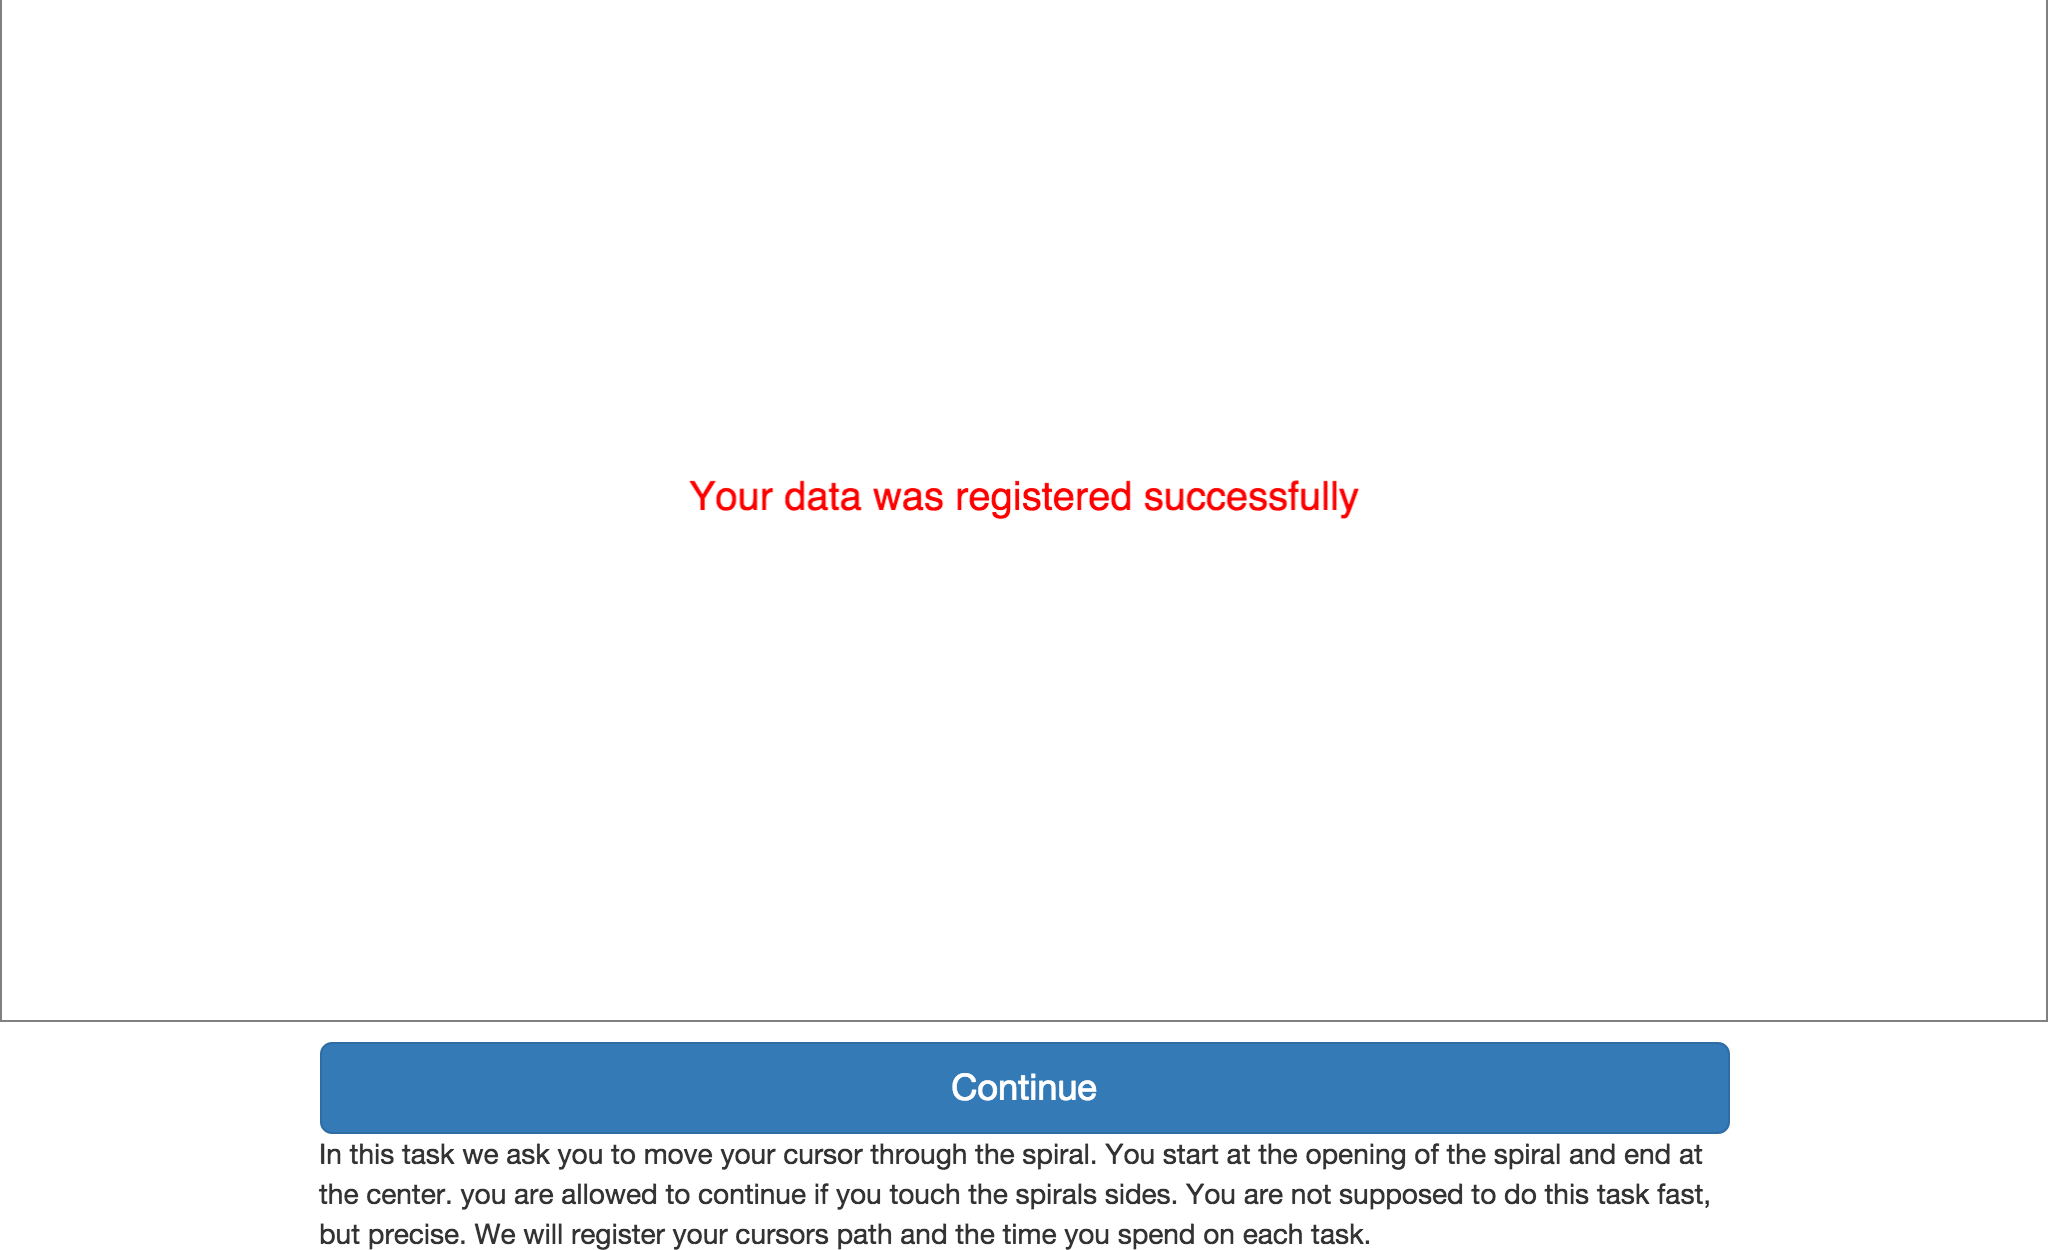
\includegraphics[width=\textwidth]{images/screenshots/ex_step_5_spiral_done}
\captionof{figure}{Eksperiment - Trin 5 - Fortsæt}
\label{fig:ex_step_5_spiral_done}
\end{minipage}

\begin{minipage}{\textwidth}
\centering
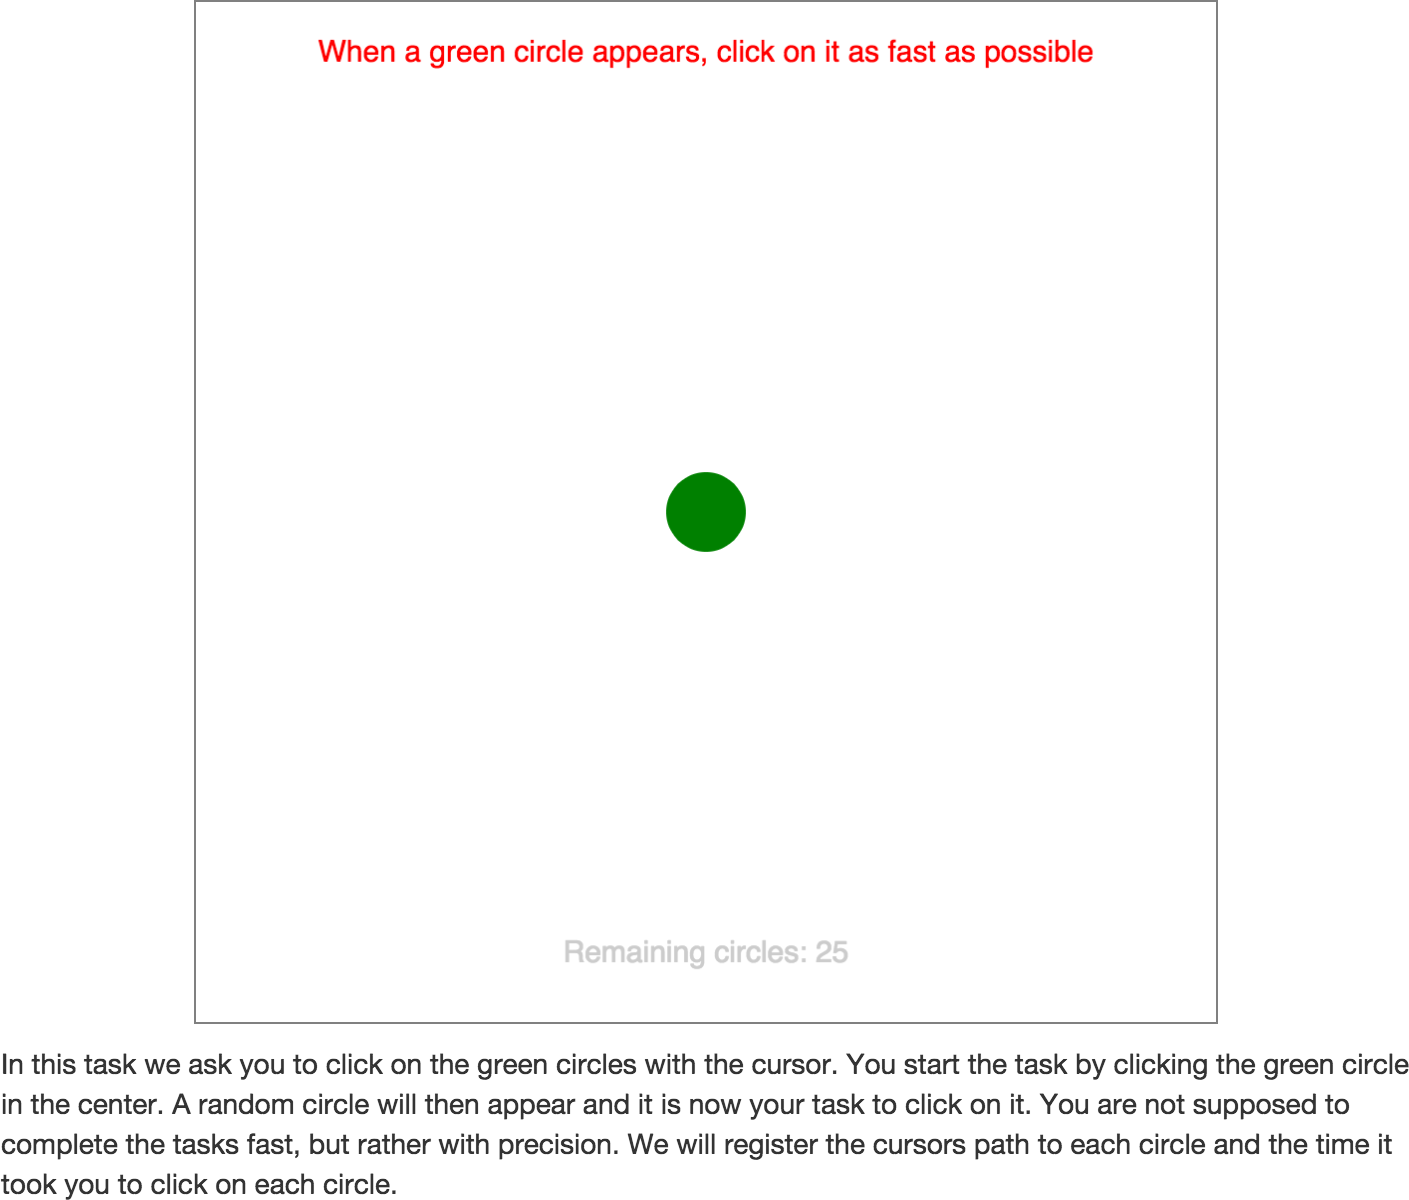
\includegraphics[height=.4\textheight]{images/screenshots/ex_step_6_pointing_start}
\captionof{figure}{Eksperiment - Trin 6 - Start}
\label{fig:ex_step_6_pointing_start}
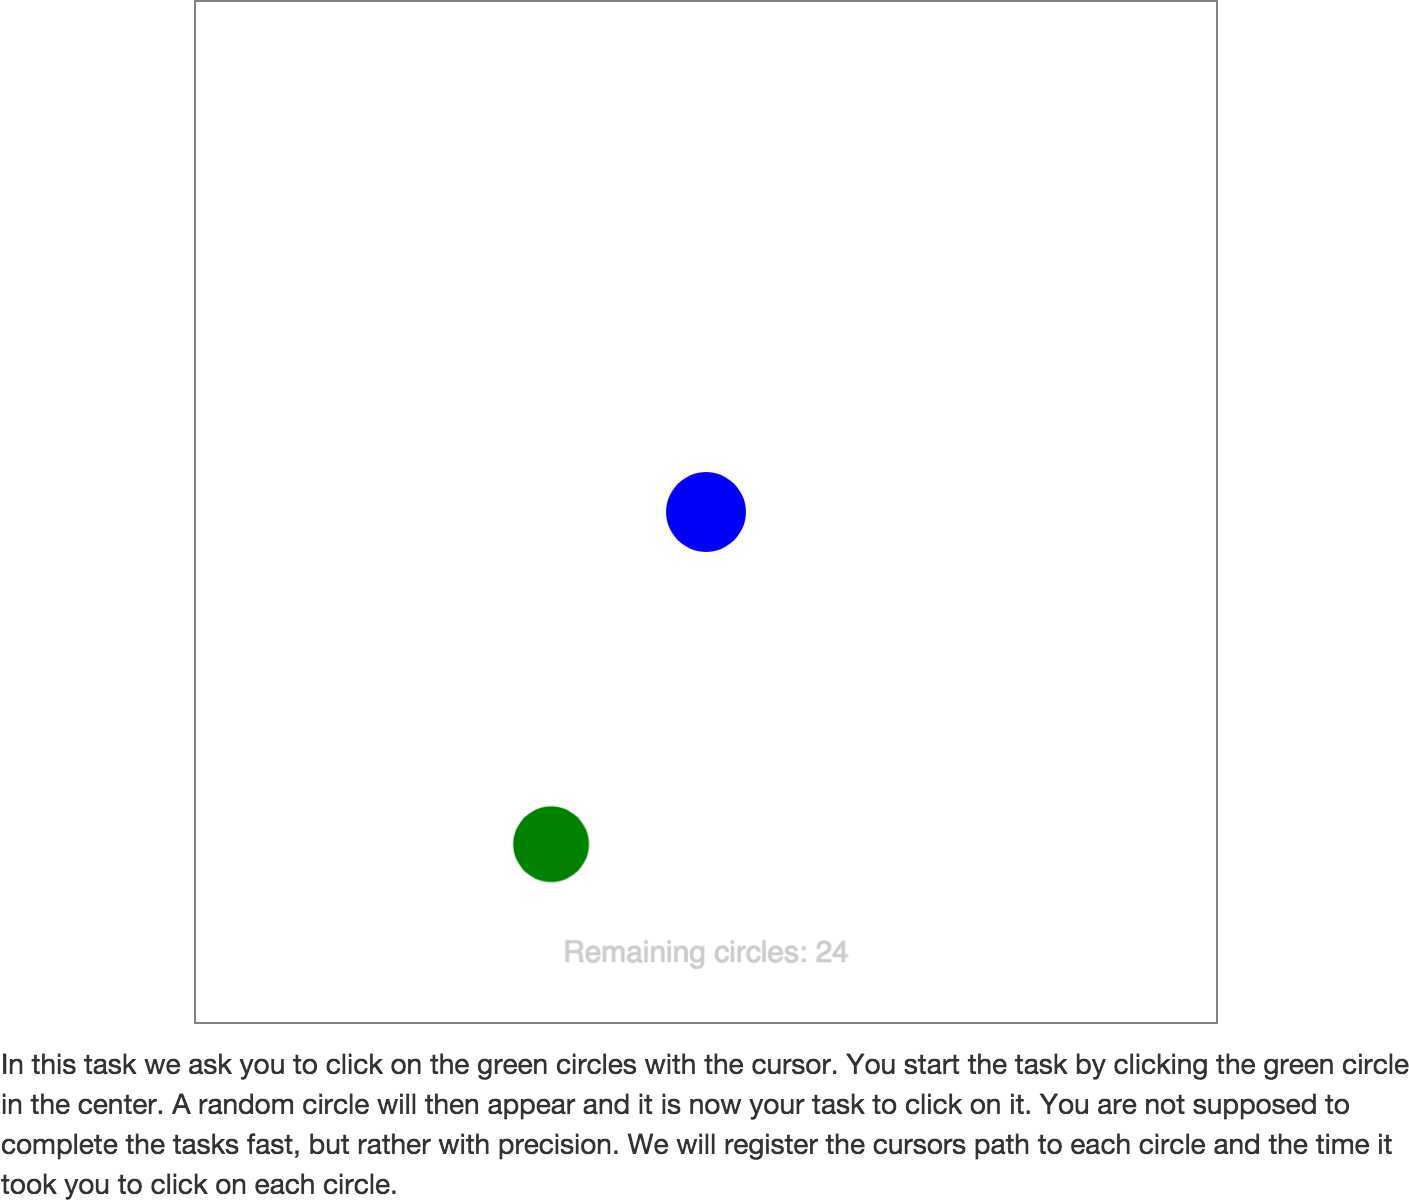
\includegraphics[height=.4\textheight]{images/screenshots/ex_step_6_pointing_target_1}
\captionof{figure}{Eksperiment - Trin 6 - Pegeeksempel 1}
\label{fig:ex_step_6_pointing_target_1}
\end{minipage}

\begin{minipage}{\textwidth}
\centering
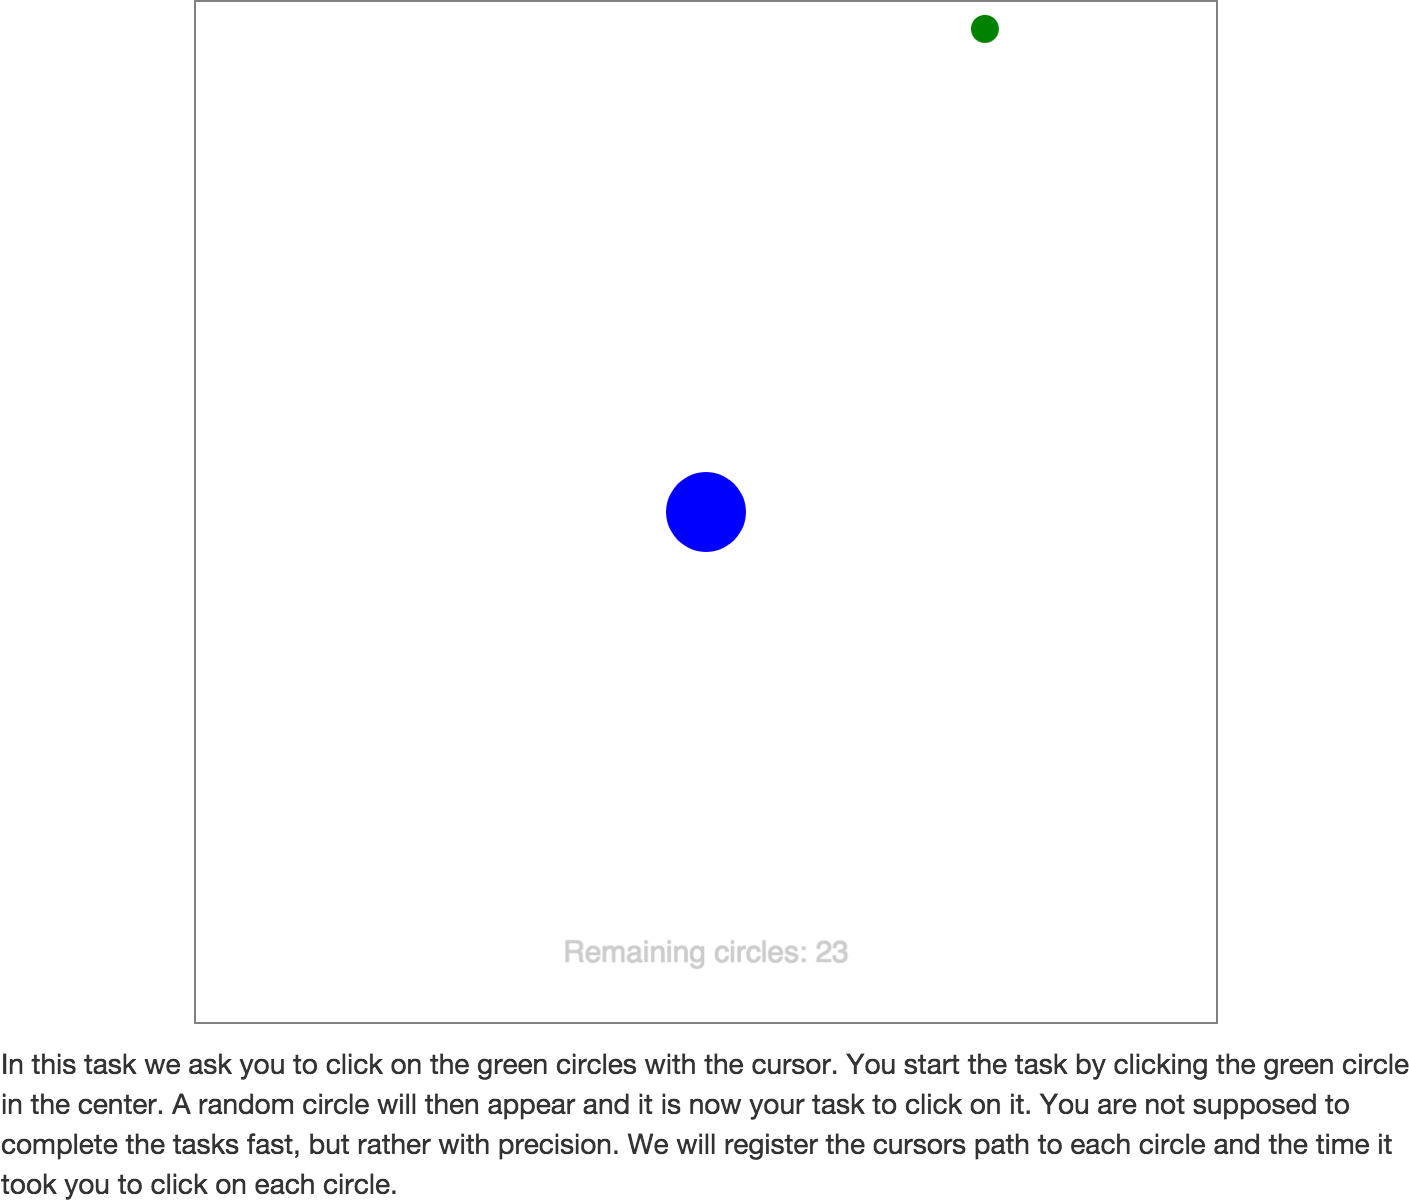
\includegraphics[height=.4\textheight]{images/screenshots/ex_step_6_pointing_target_2}
\captionof{figure}{Eksperiment - Trin 6 - Pegeeksempel 2}
\label{fig:ex_step_6_pointing_target_2}
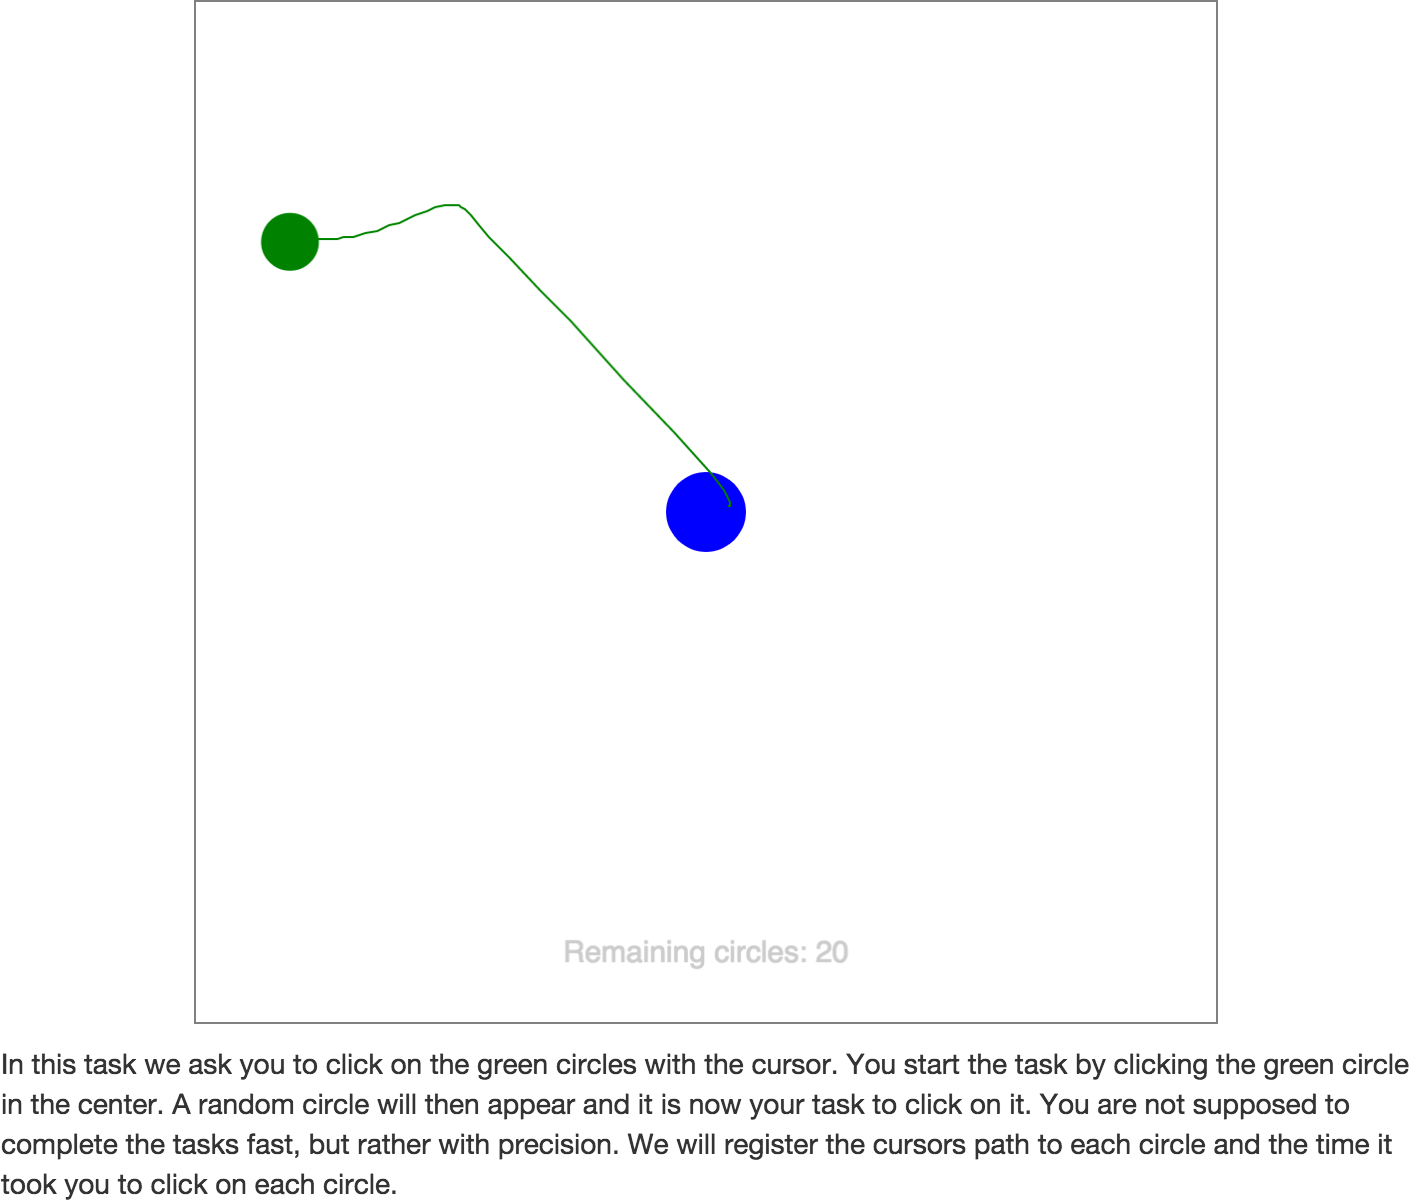
\includegraphics[height=.4\textheight]{images/screenshots/ex_step_6_pointing_path}
\captionof{figure}{Eksperiment - Trin 6 - Pegebane}
\label{fig:ex_step_6_pointing_path}
\end{minipage}

\begin{minipage}{\textwidth}
\centering
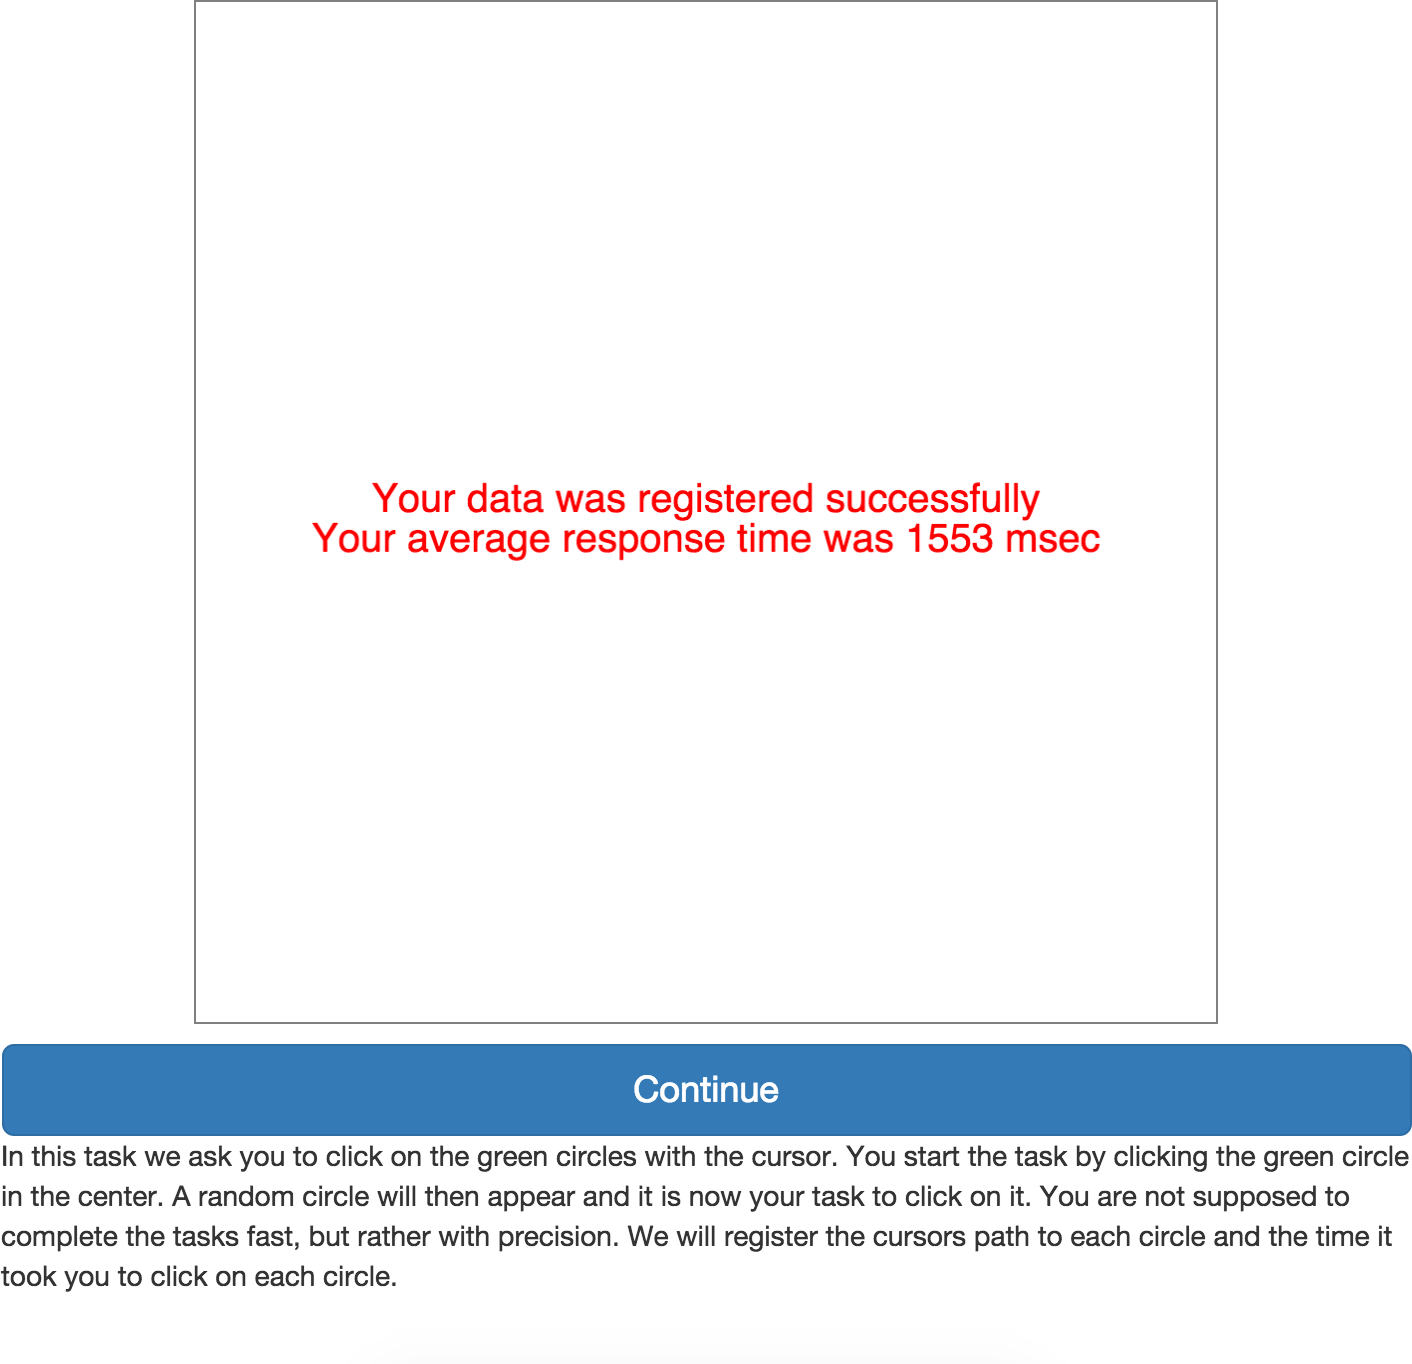
\includegraphics[height=.4\textheight]{images/screenshots/ex_step_6_pointing_done}
\captionof{figure}{Eksperiment - Trin 6 - Færdig}
\label{fig:ex_step_6_pointing_done}
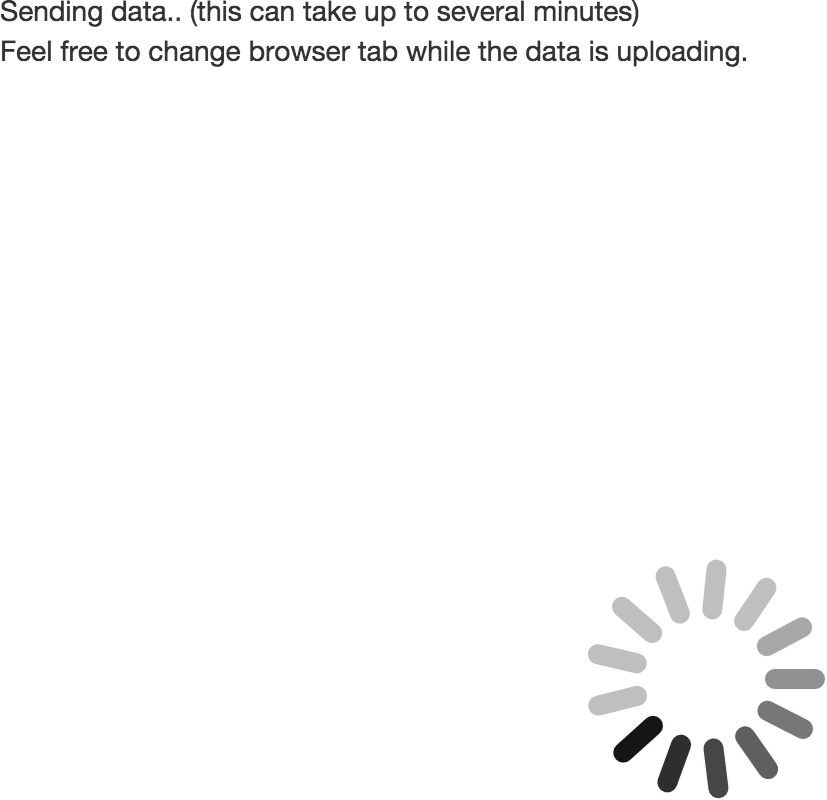
\includegraphics[height=.4\textheight]{images/screenshots/ex_step_7_sending}
\captionof{figure}{Eksperiment - Trin 7 - Sender}
\label{fig:ex_step_7_sending}
\end{minipage}

%-- Drejebog --%
\chapter{Drejebog for laboratorieeksperiment}
\label{sec:drejebog}
\subsection*{Udstyr}
\begin{itemize}
\item{Computer med Google Chrome browseren}
\item{Mus og musemåtte}
\end{itemize}
\subsection*{Før test}
\begin{itemize}
\item{P1 rækker testdeltager et A4 ark med følgende tekst;
      \\\textit{"Vi er i gang med et bachelorprojekt, der handler om Fitts' lov. Det er en model, som beskriver det menneskelige motoriske systems kapacitet. I denne sammenhæng, hvordan tiden til at ramme et mål på skærmen ved hjælp af musen afhænger af afstanden til og størrelsen på målet. Vi har derfor udviklet dette eksperiment for at indsamle data. Du vil undervejs blive stillet forskellige opgaver, som du skal forsøge at løse."}}
\item{P1 beder testdeltageren om at teste musens følsomhed ved at køre frit rundt med musen. Der gøres opmærksom på, at testdeltageren gerne må ændre følsomheden, hvis de føler for det.}
\item{P2 starter en Google Chrome browser og peger den på følgende adresse:\\ \url{http://codeit.io/bachelor/survey.html}.}
\end{itemize}
\subsection*{Under test}
\begin{itemize}
\item{P2 beder testdeltageren om at tage plads ved den klargjorte computer.}
\item{P2 beder testdeltageren om at udfylde formularen på skærmen med information.}
\item{P2 gør opmærksom på, at der skal skrives 'testperson x', hvor 'x' er nummeret på testpersonen, i feltet om hvorfra de hørte om siden (dette er for senere at kunne finde dem i databasen)}
\item{P1 fortæller testdeltageren, at de gerne må gå i gang med opgaverne og kan stille spørgsmål undervejs, hvis de har brug for det.}
\end{itemize}
\subsection*{Efter test}
\begin{itemize}
\item{P1 fortæller testdeltageren, hvordan  deres data vil blive brugt;
\\\textit{"Tak fordi du ville deltage i forsøget og hjælpe os med vores projekt. De baner du undervejs har foretaget for at udføre opgaverne vil blive brugt til at analysere, hvorvidt de stemmer overens med forskellige formuleringer af Fitt's lov, eller om der kan findes en forbedret formulering"}.}
\end{itemize}

%-- Tekst til crowdsourcing --%
\chapter{Tekst til crowdsourcing}
\label{sec:crowdsource-text}
For at crowdsource vores eksperiment har vi delt følgende tekst:
\\\\\textit{"Hej,\\ vi er tre datalogi studerende ved Københavns Universitet, som er i gang med vores bacheloropgave. For at kunne have nogle data at analysere, har vi lavet denne hjemmeside med 'pegeopgaver'. Opgaverne tager cirka 10-15 minutter at udføre og er skidesjove! Det ville derfor være utrolig værdsat, hvis du ville gå ind på følgende hjemmeside \url{http://www.codeit.io/bachelor/index.html} og udføre opgaverne. Deltag senest d. 27/04.
\\Eventulle spørgsmål kan henvendes til en af os på;\\bdj816@alumni.ku.dk, hmd200@alumni.ku.dk, qgf142@alumni.ku.dk"}
\\\\\textit{"Hello,\\ We are three computer science students at the University of Copenhagen, who are currently working on our bachelor thesis. We have made the following webpage with 'pointingtasks' in order to have some data to analyze. The tasks takes approximately 10-15 minuttes and are super fun! It would therefore be very appreciated if you would visit the webpage at \url{http://www.codeit.io/bachelor/index.html} and complete the tasks. Deadline is the 27th of April.
\\Any questions regarding the projects are welcome at either of these emails;\\bdj816@alumni.ku.dk, hmd200@alumni.ku.dk, qgf142@alumni.ku.dk"}

%-- R-kode --%
\chapter{R-kode fra analyse}
\label{sec:r-code}
\lstinputlisting[language=R]{main.r}

%-- Kvalitativ analyse --%
\chapter{Testdeltageres bevægelsesbaner}
\label{sec:movementlines}
\begin{minipage}{\textwidth}
	\begin{minipage}{0.5\linewidth}
		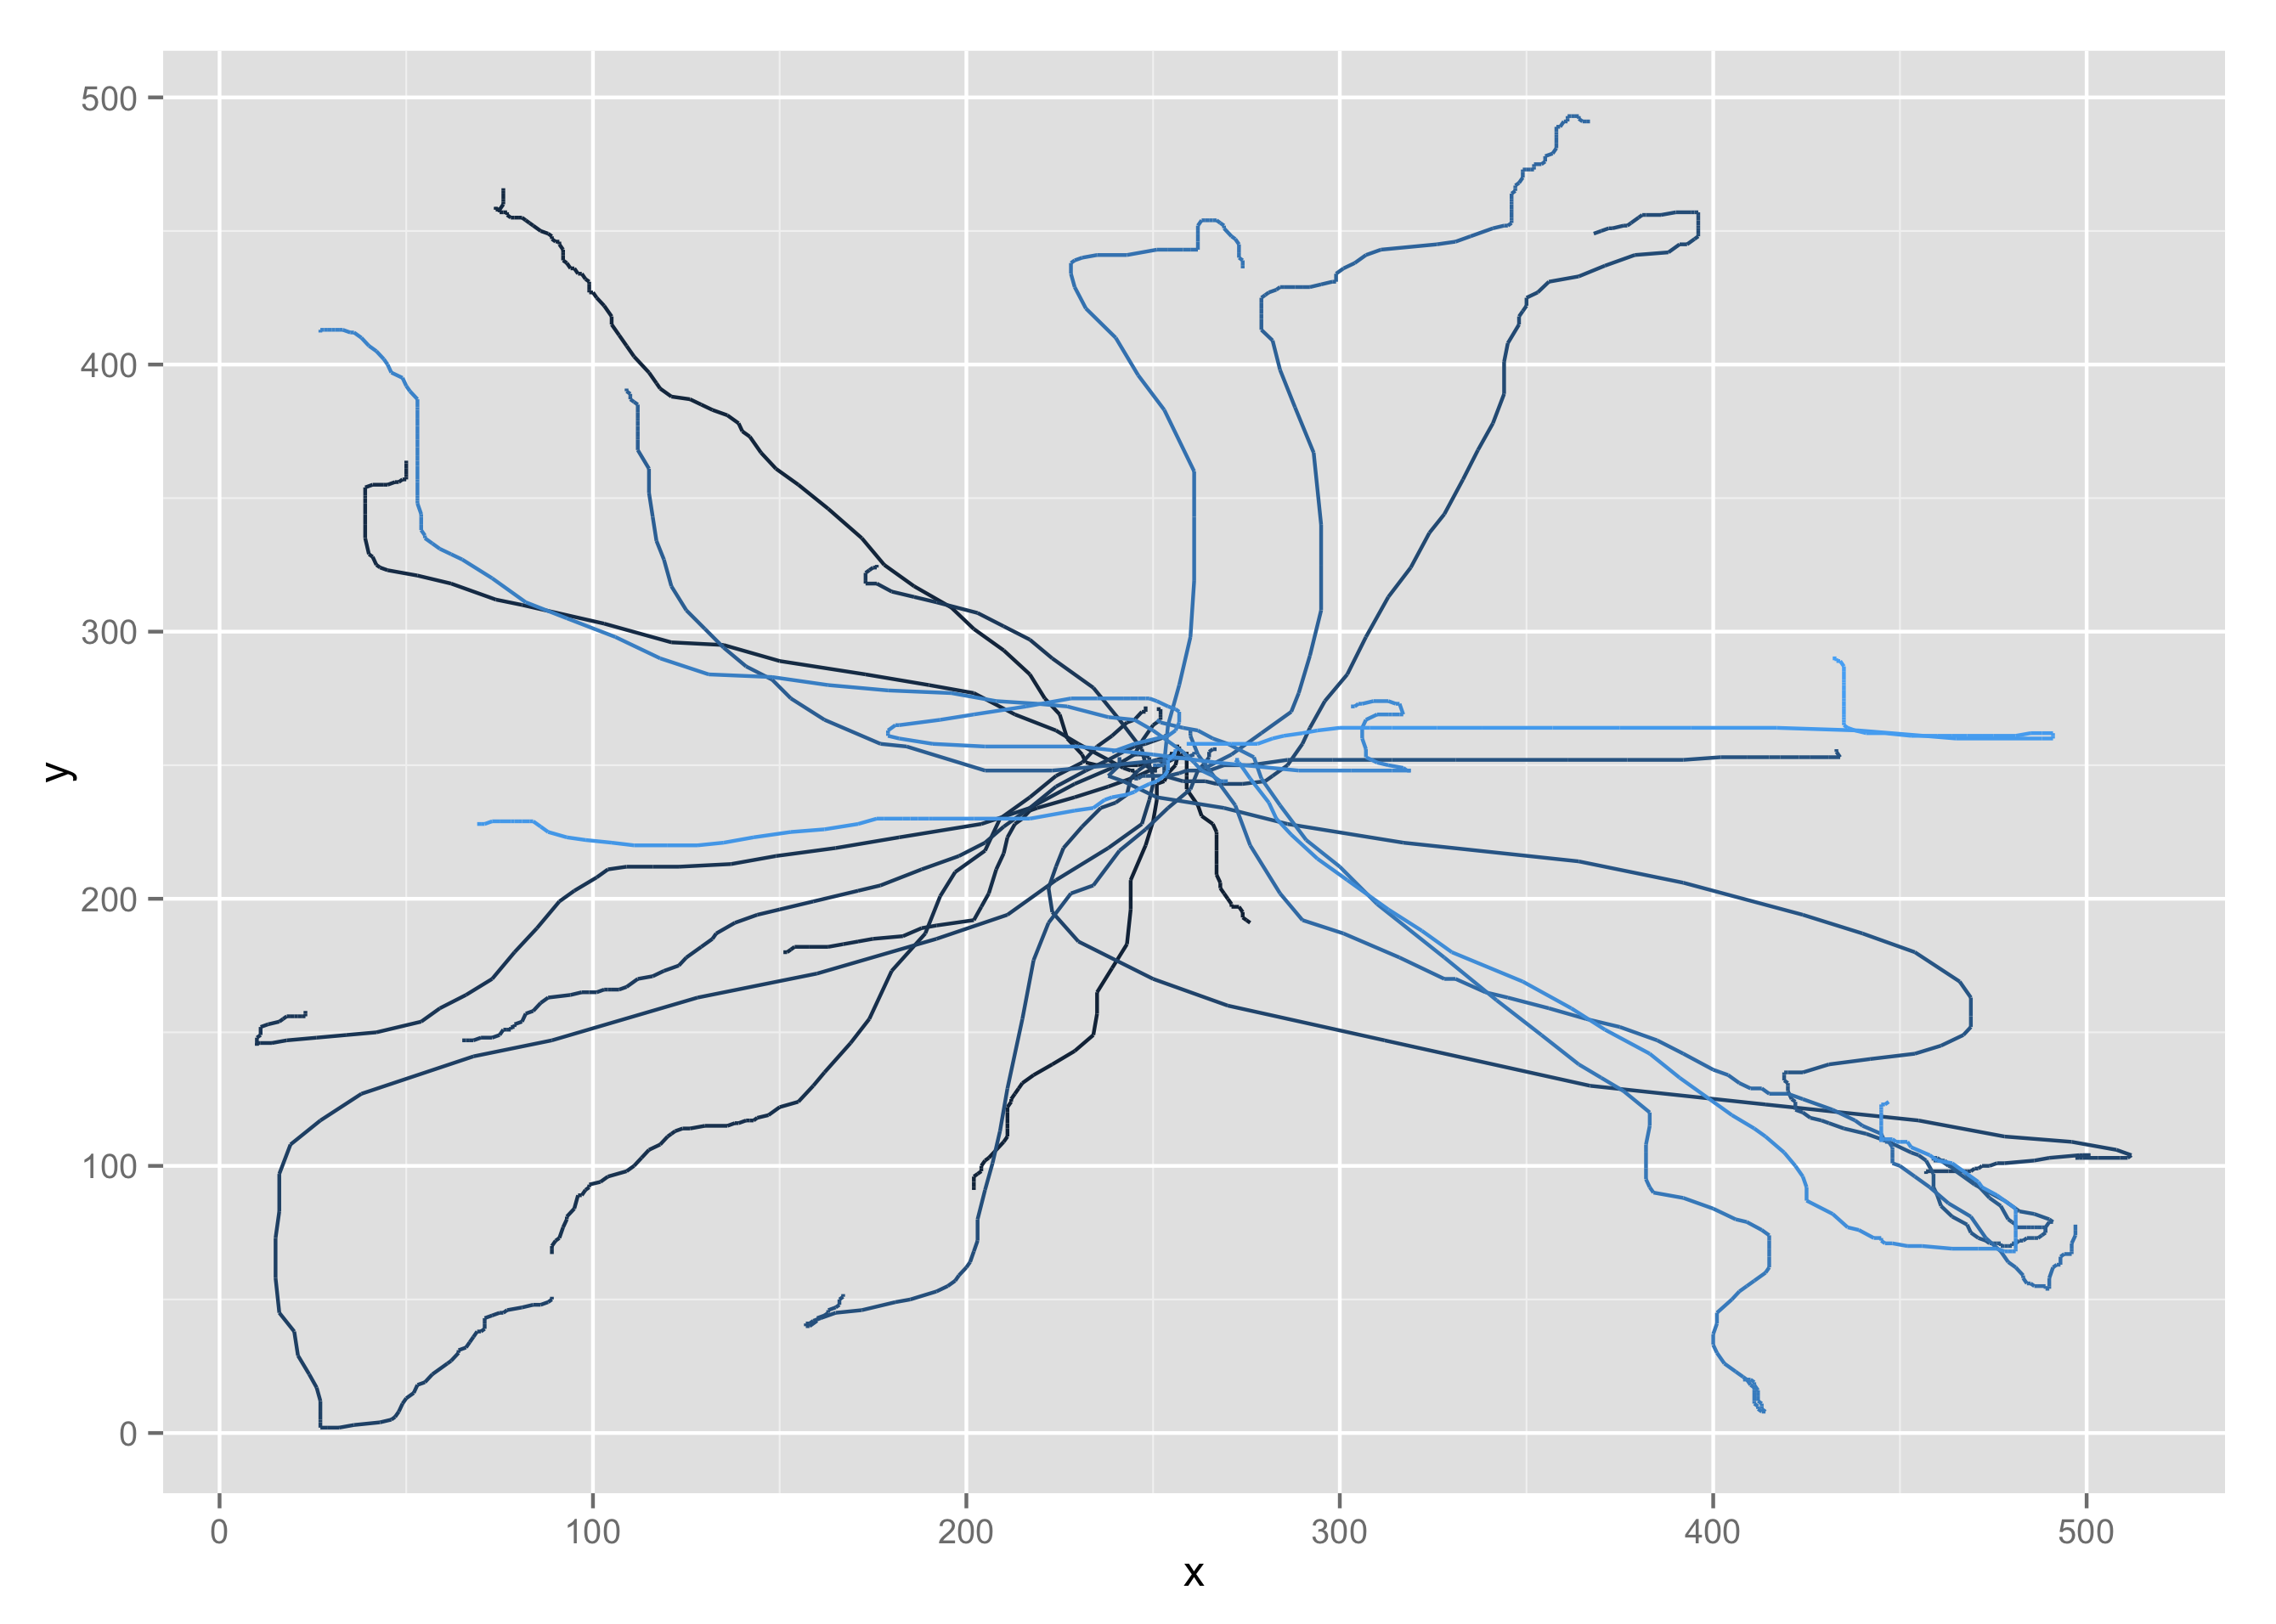
\includegraphics[width=\linewidth]{images/plots/plot_analysis_qualitative_77}
	\end{minipage}
	\begin{minipage}{0.5\linewidth}
		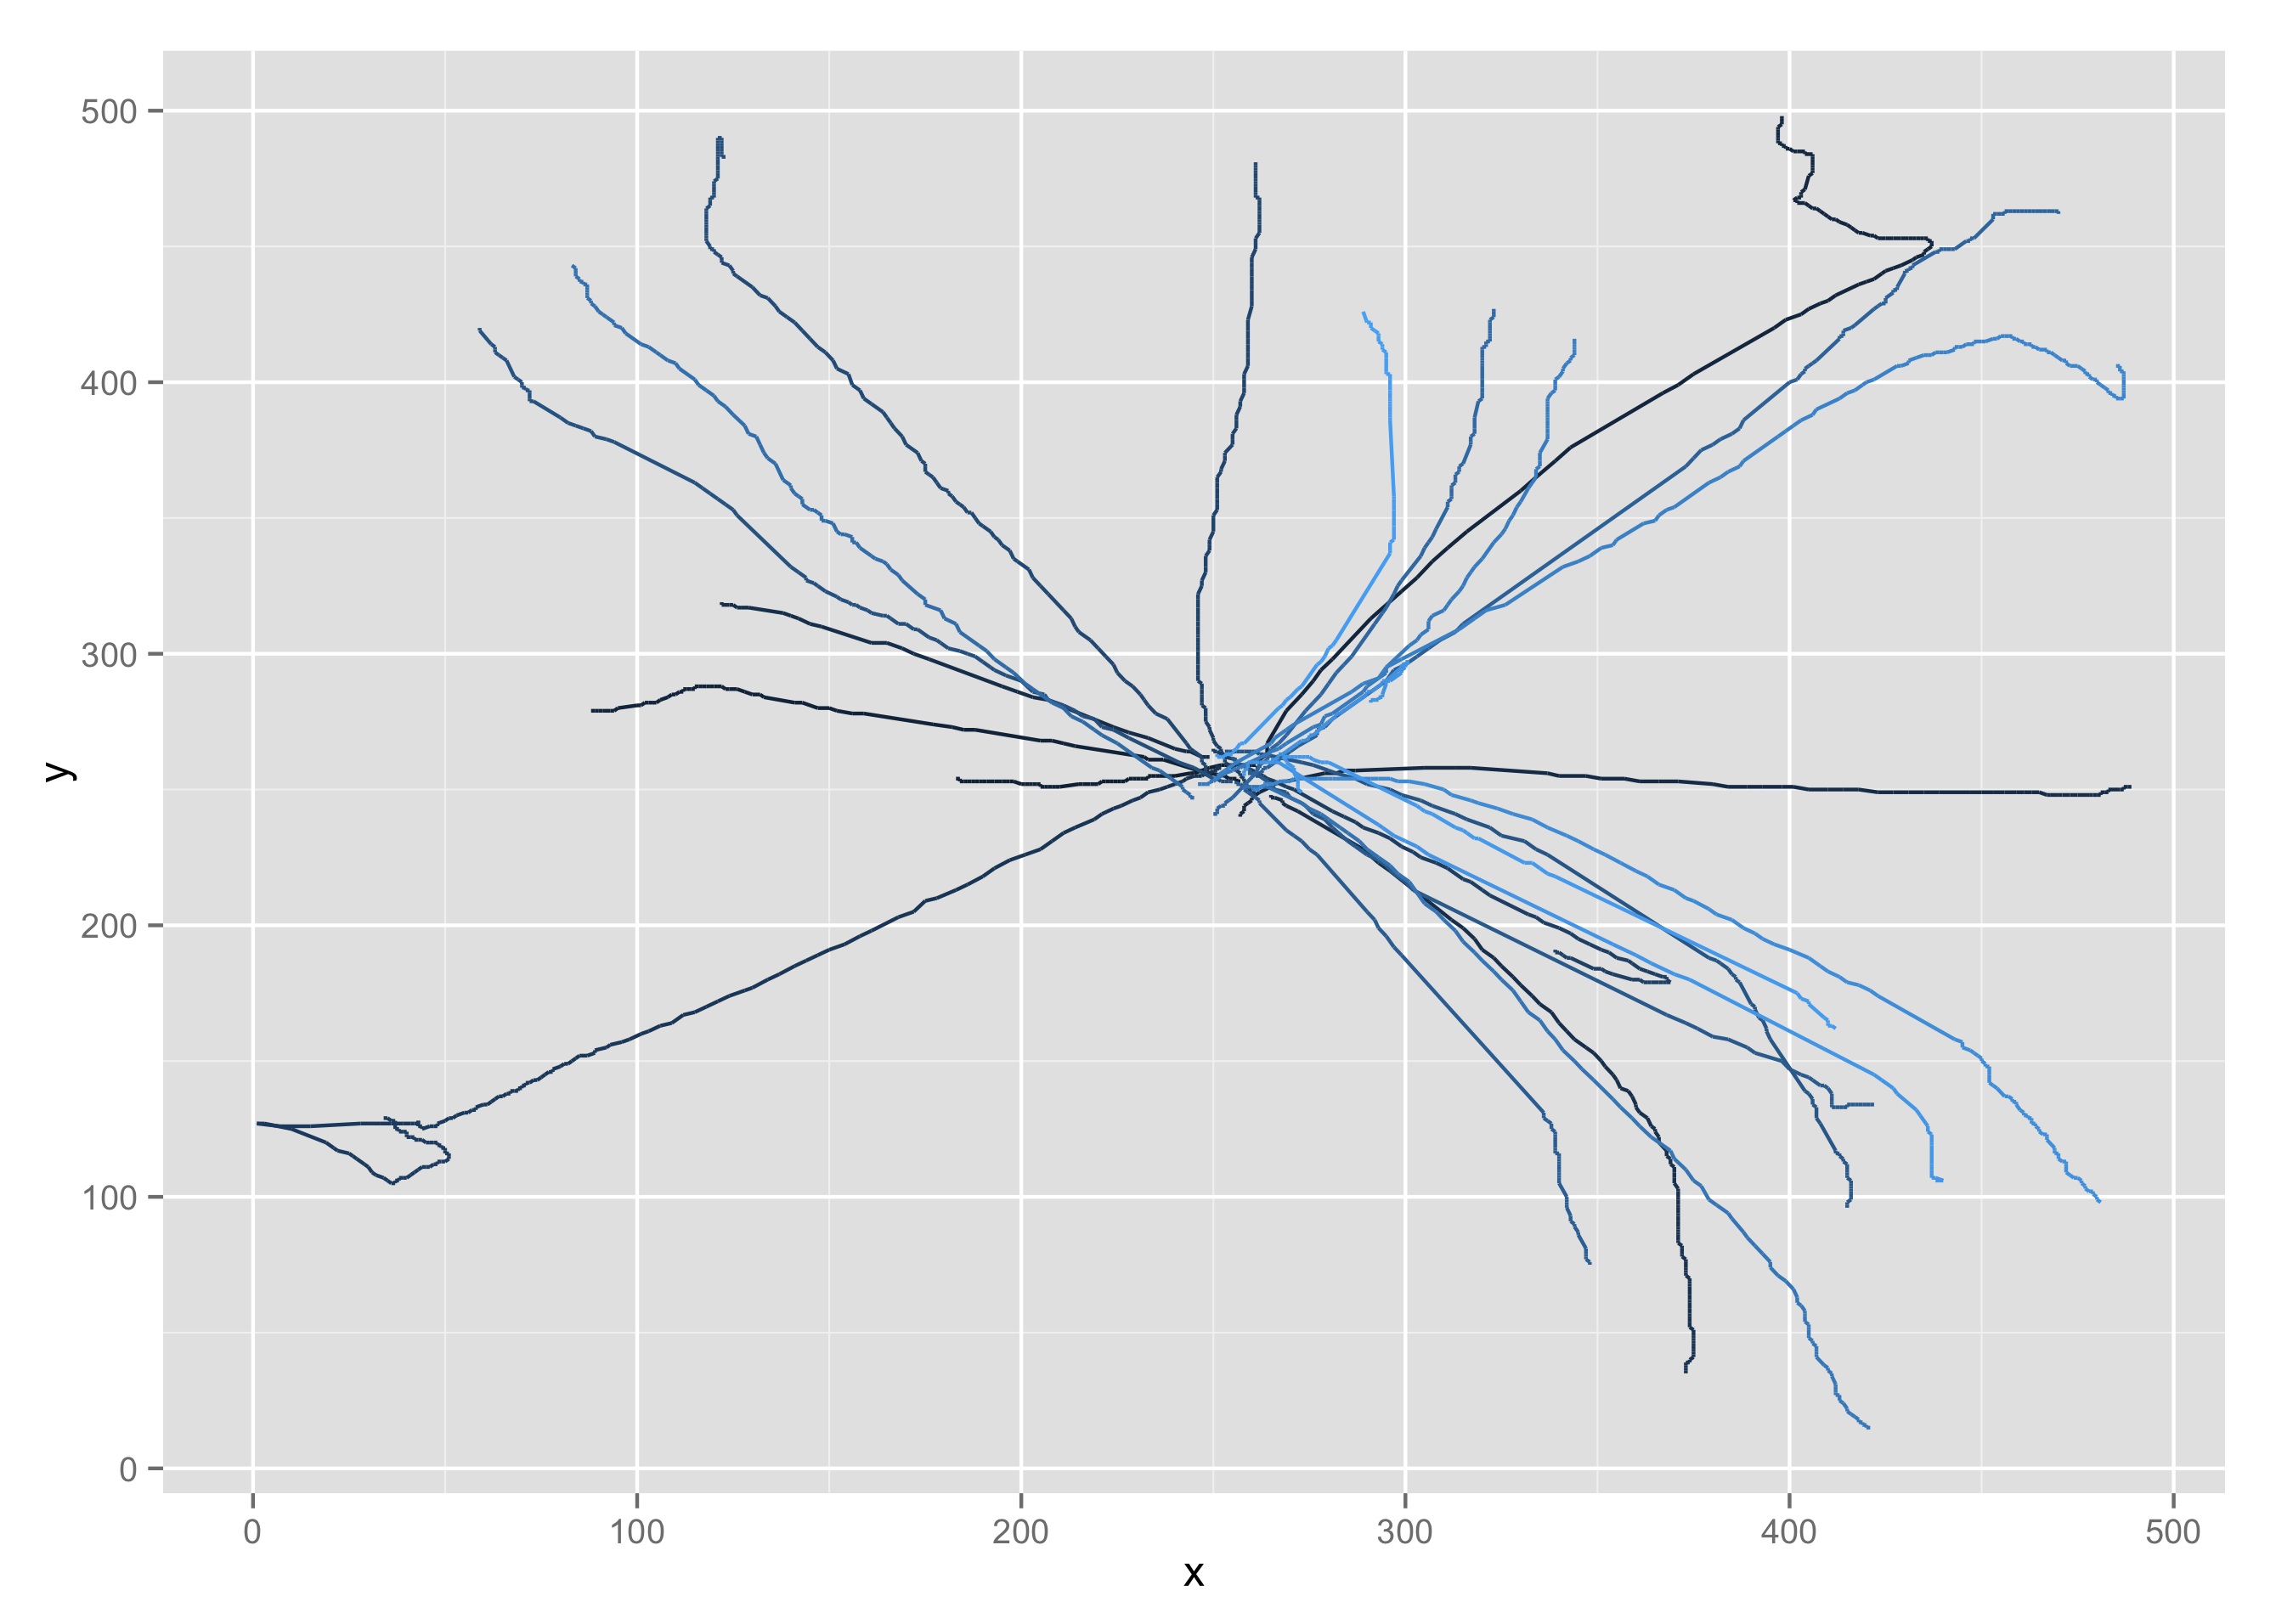
\includegraphics[width=\linewidth]{images/plots/plot_analysis_qualitative_45}
	\end{minipage}
	\begin{minipage}{0.5\linewidth}
		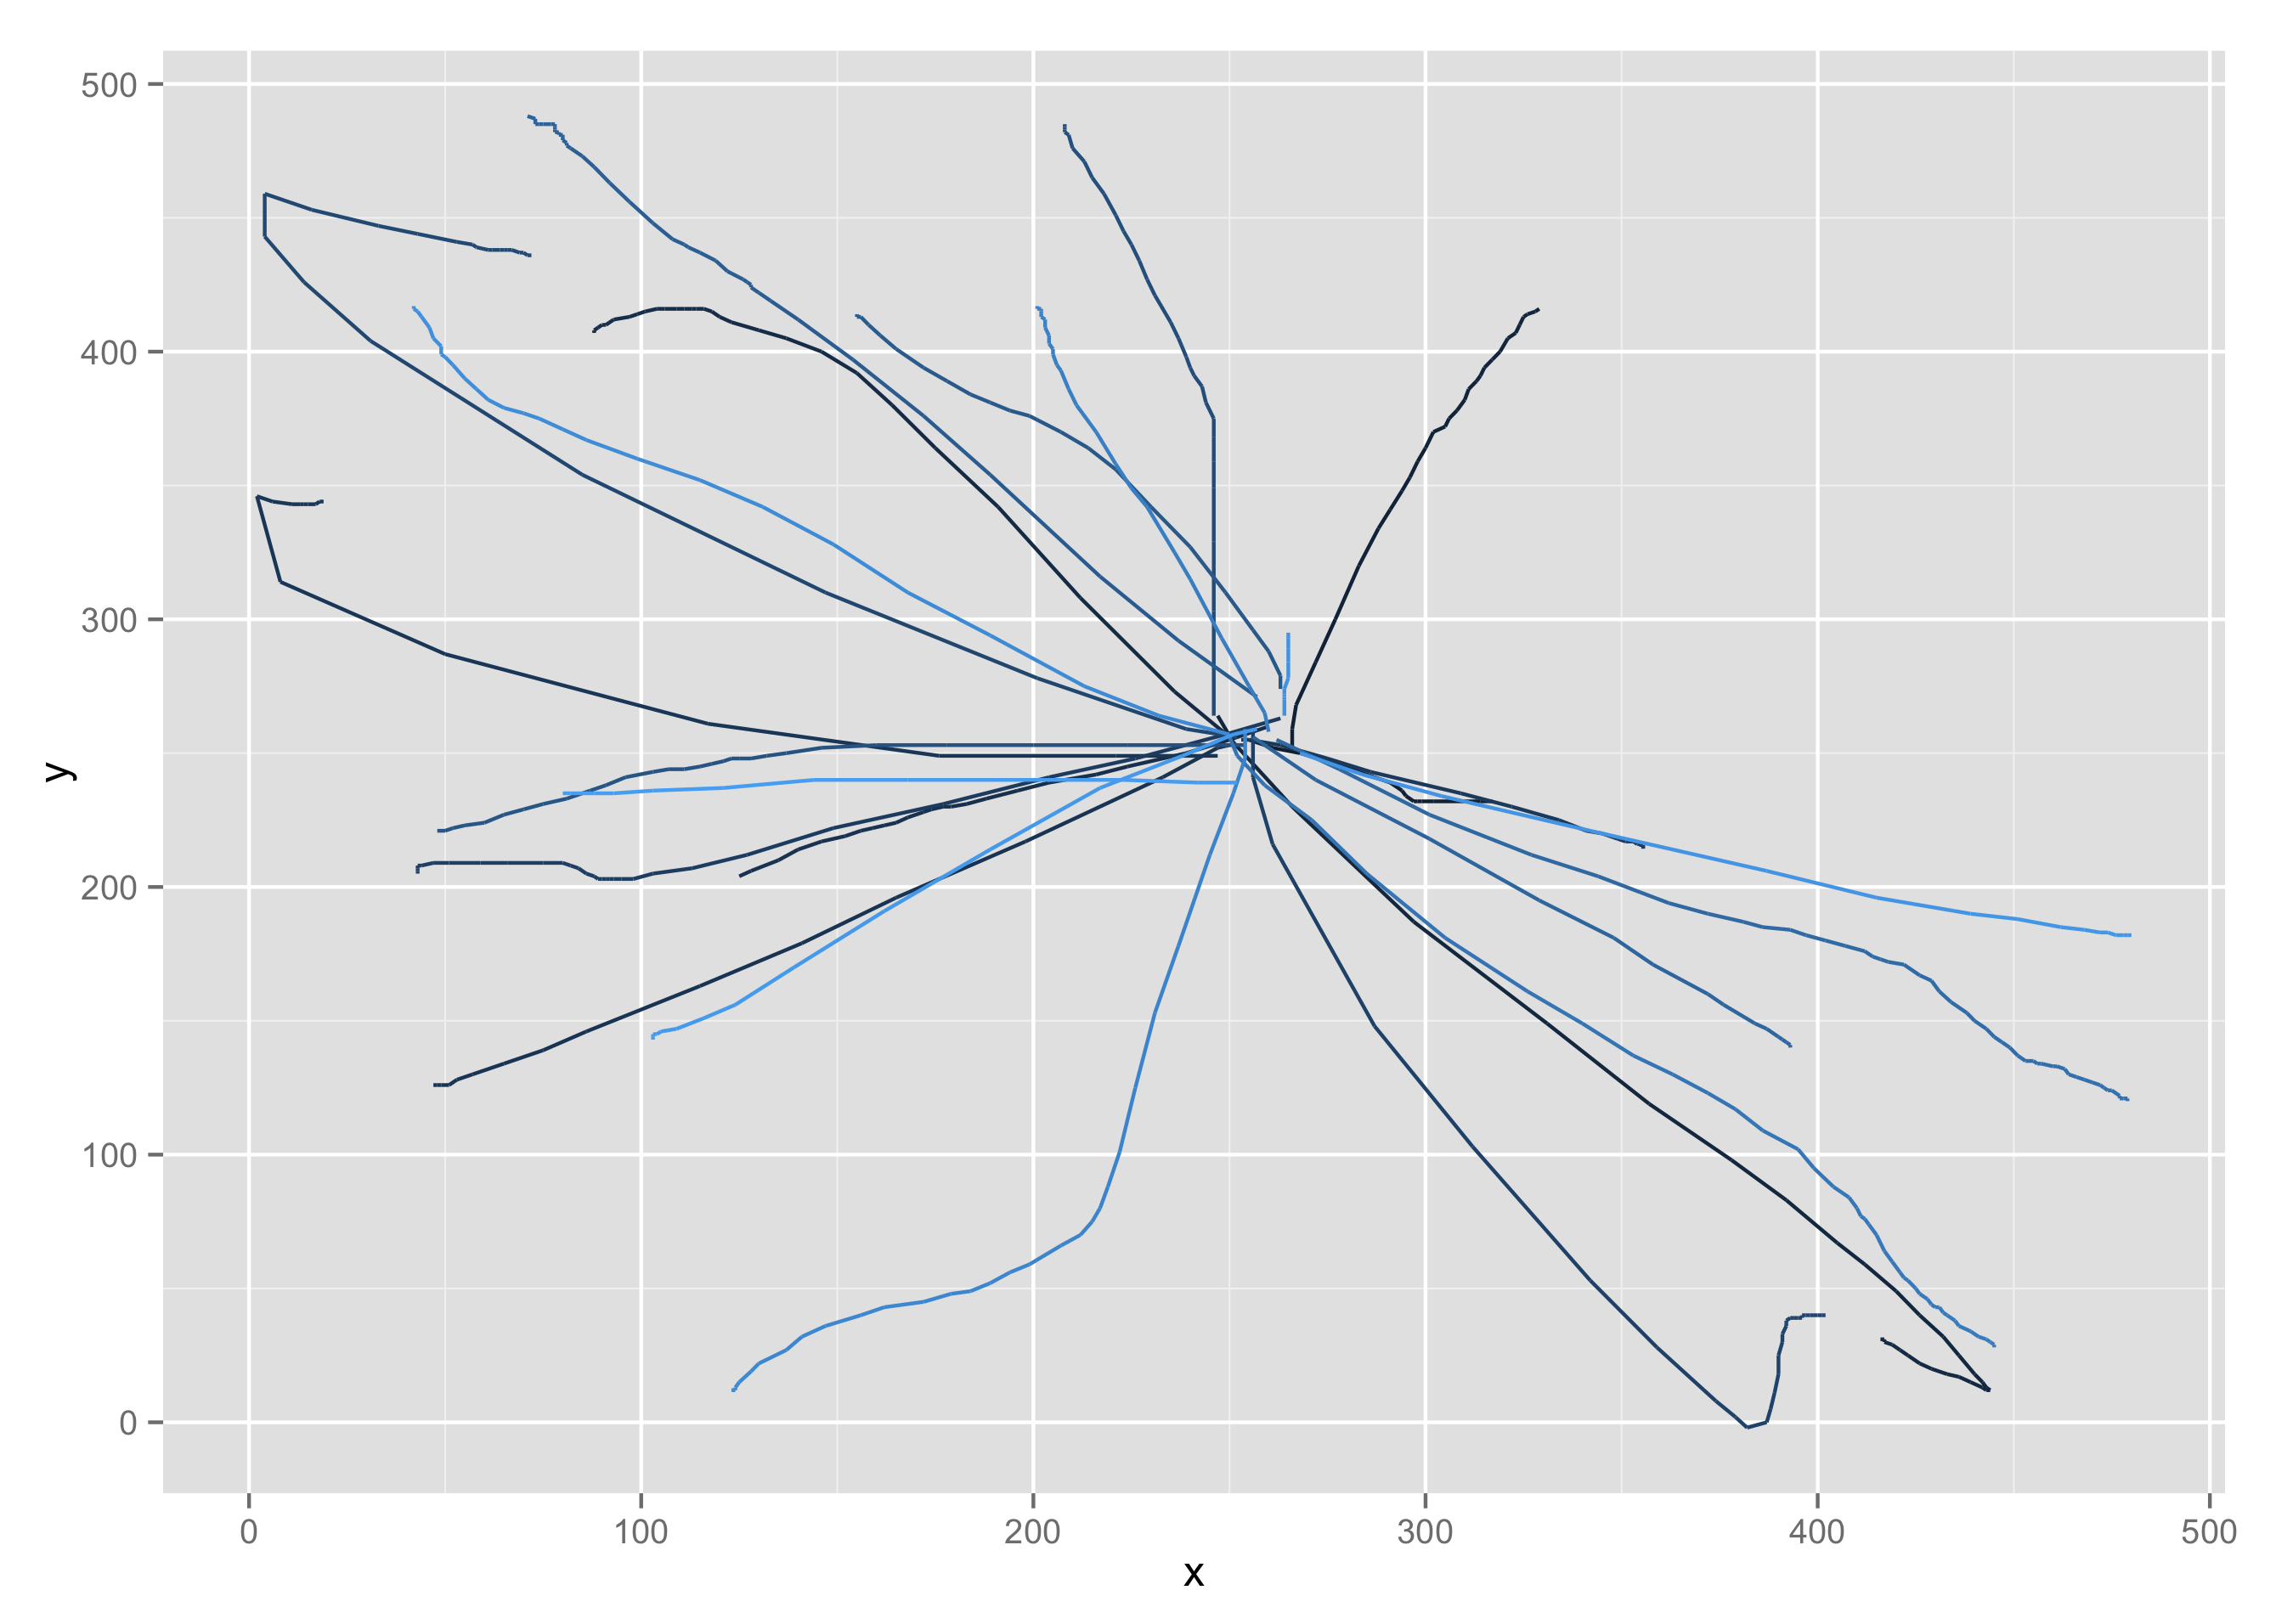
\includegraphics[width=\linewidth]{images/plots/plot_analysis_qualitative_225}
	\end{minipage}
	\begin{minipage}{0.5\linewidth}
		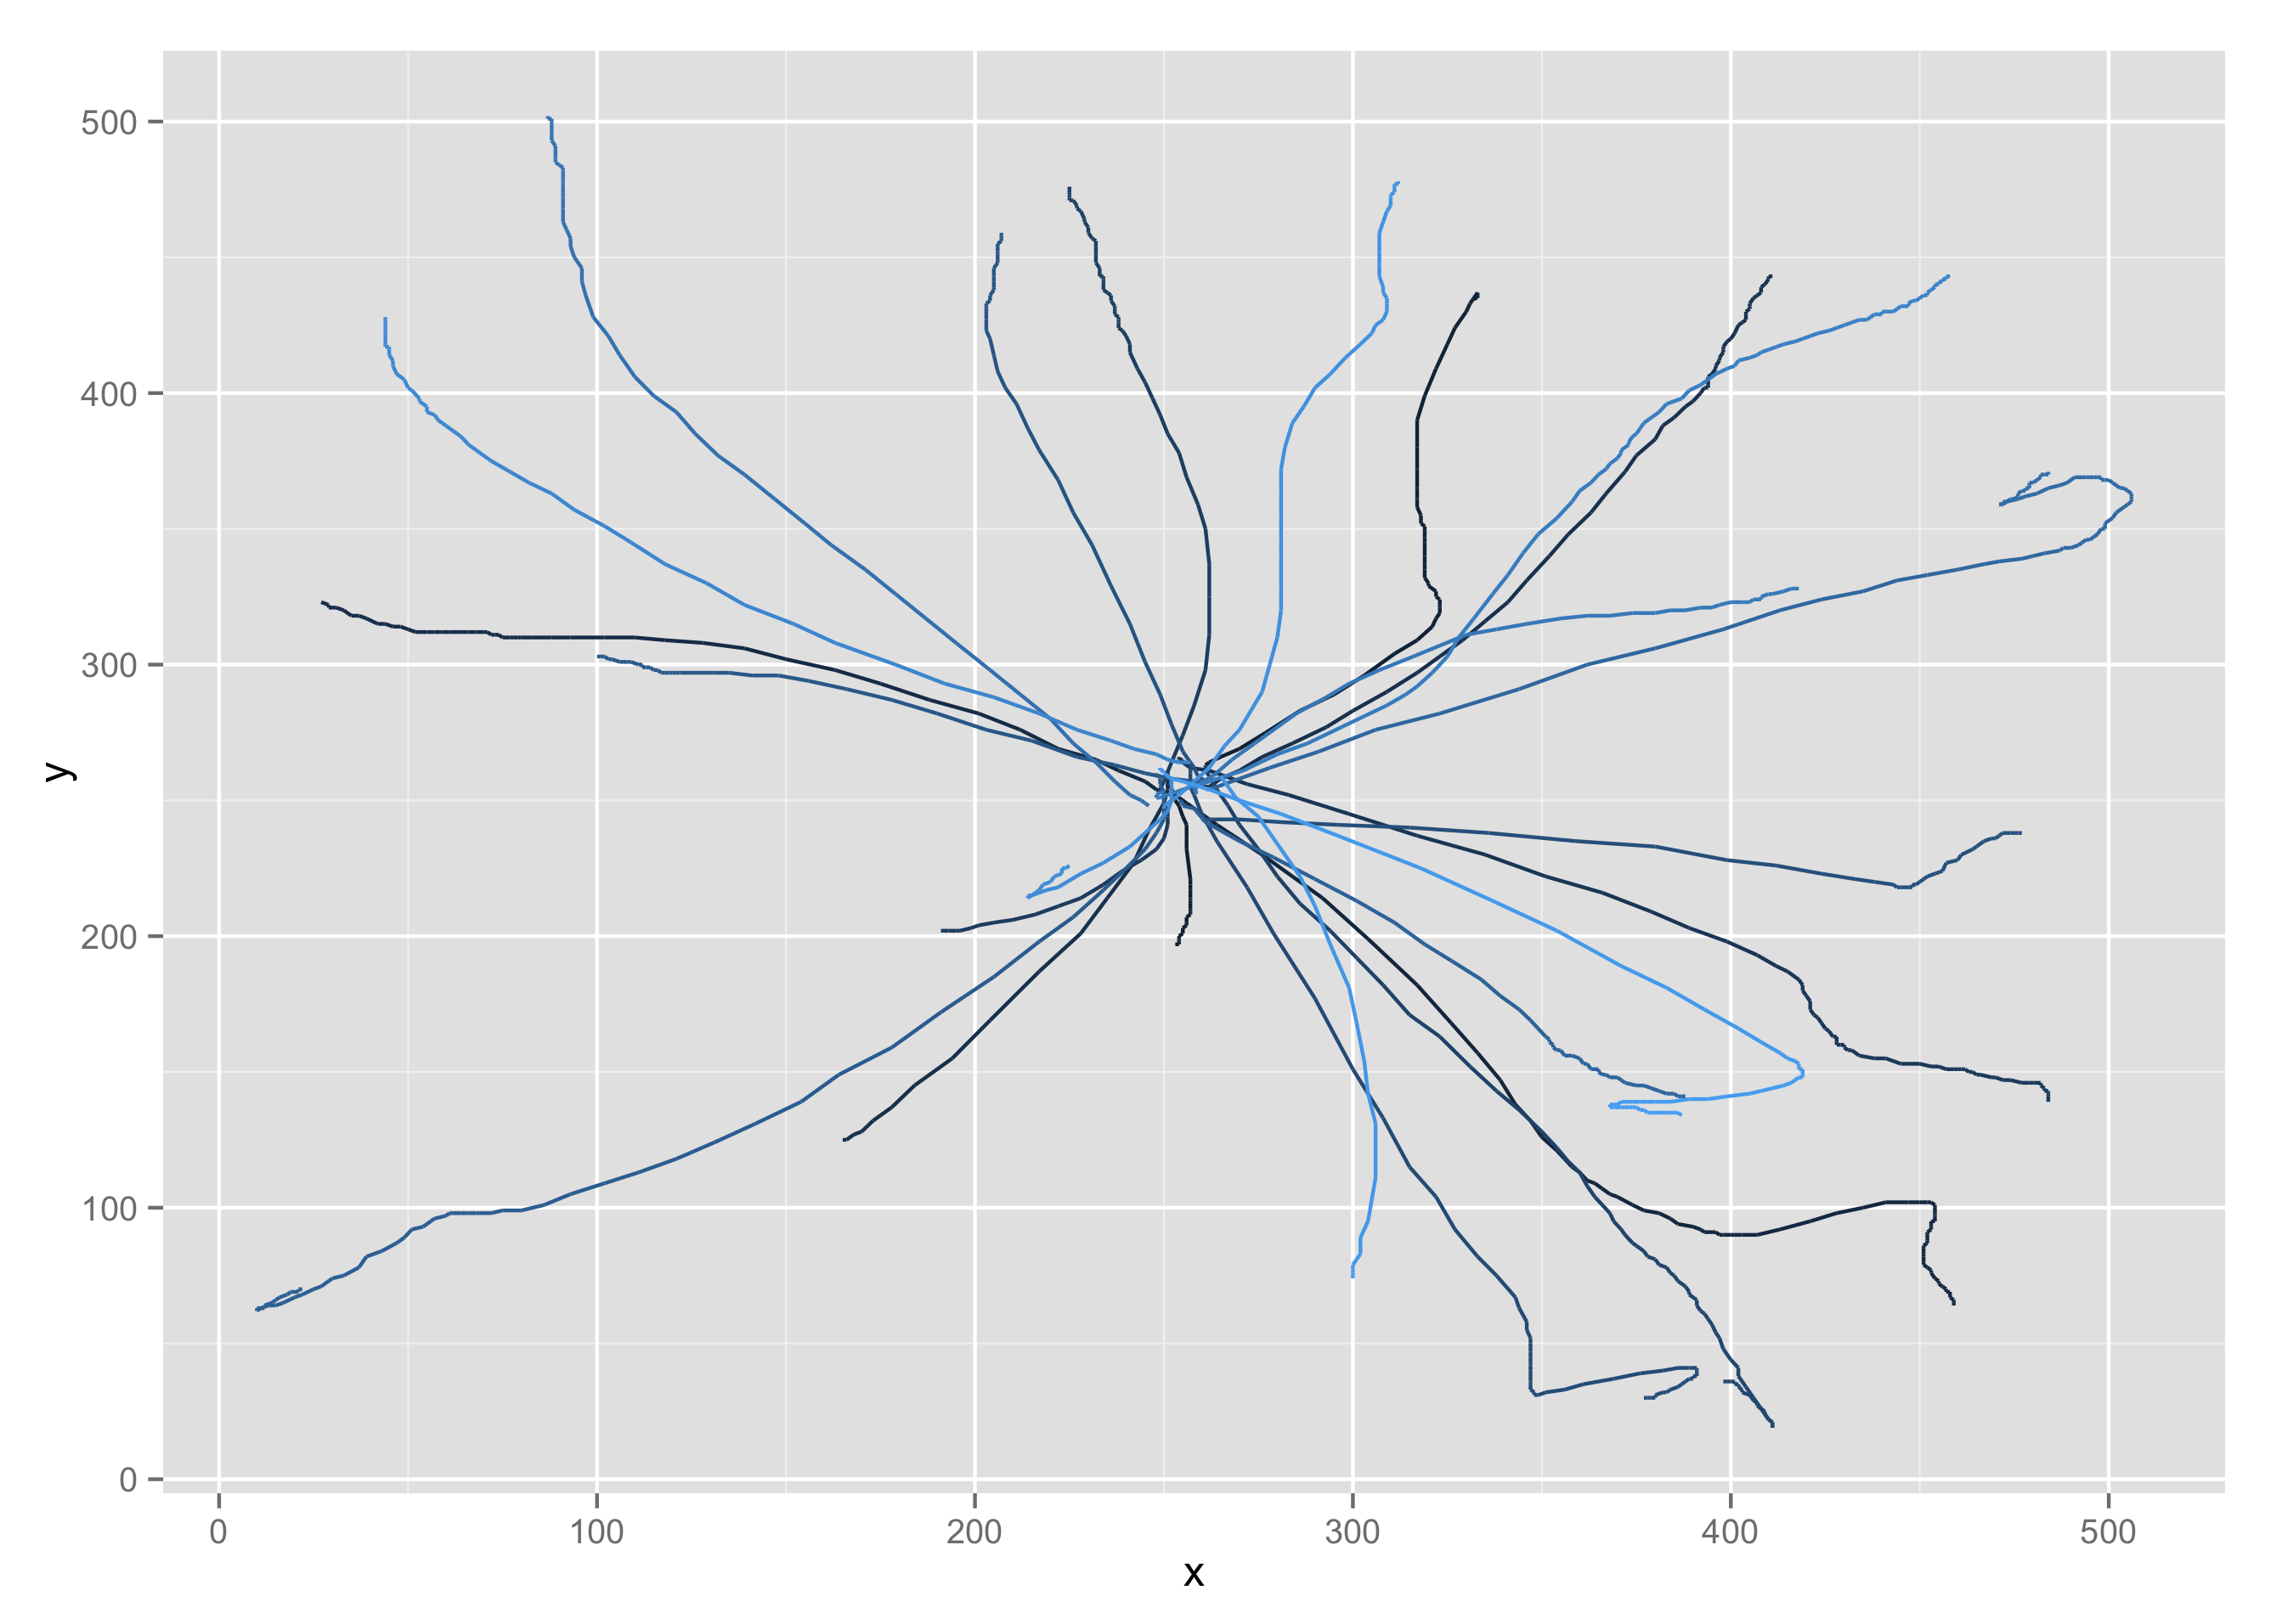
\includegraphics[width=\linewidth]{images/plots/plot_analysis_qualitative_161}
	\end{minipage}
	\begin{minipage}{0.5\linewidth}
		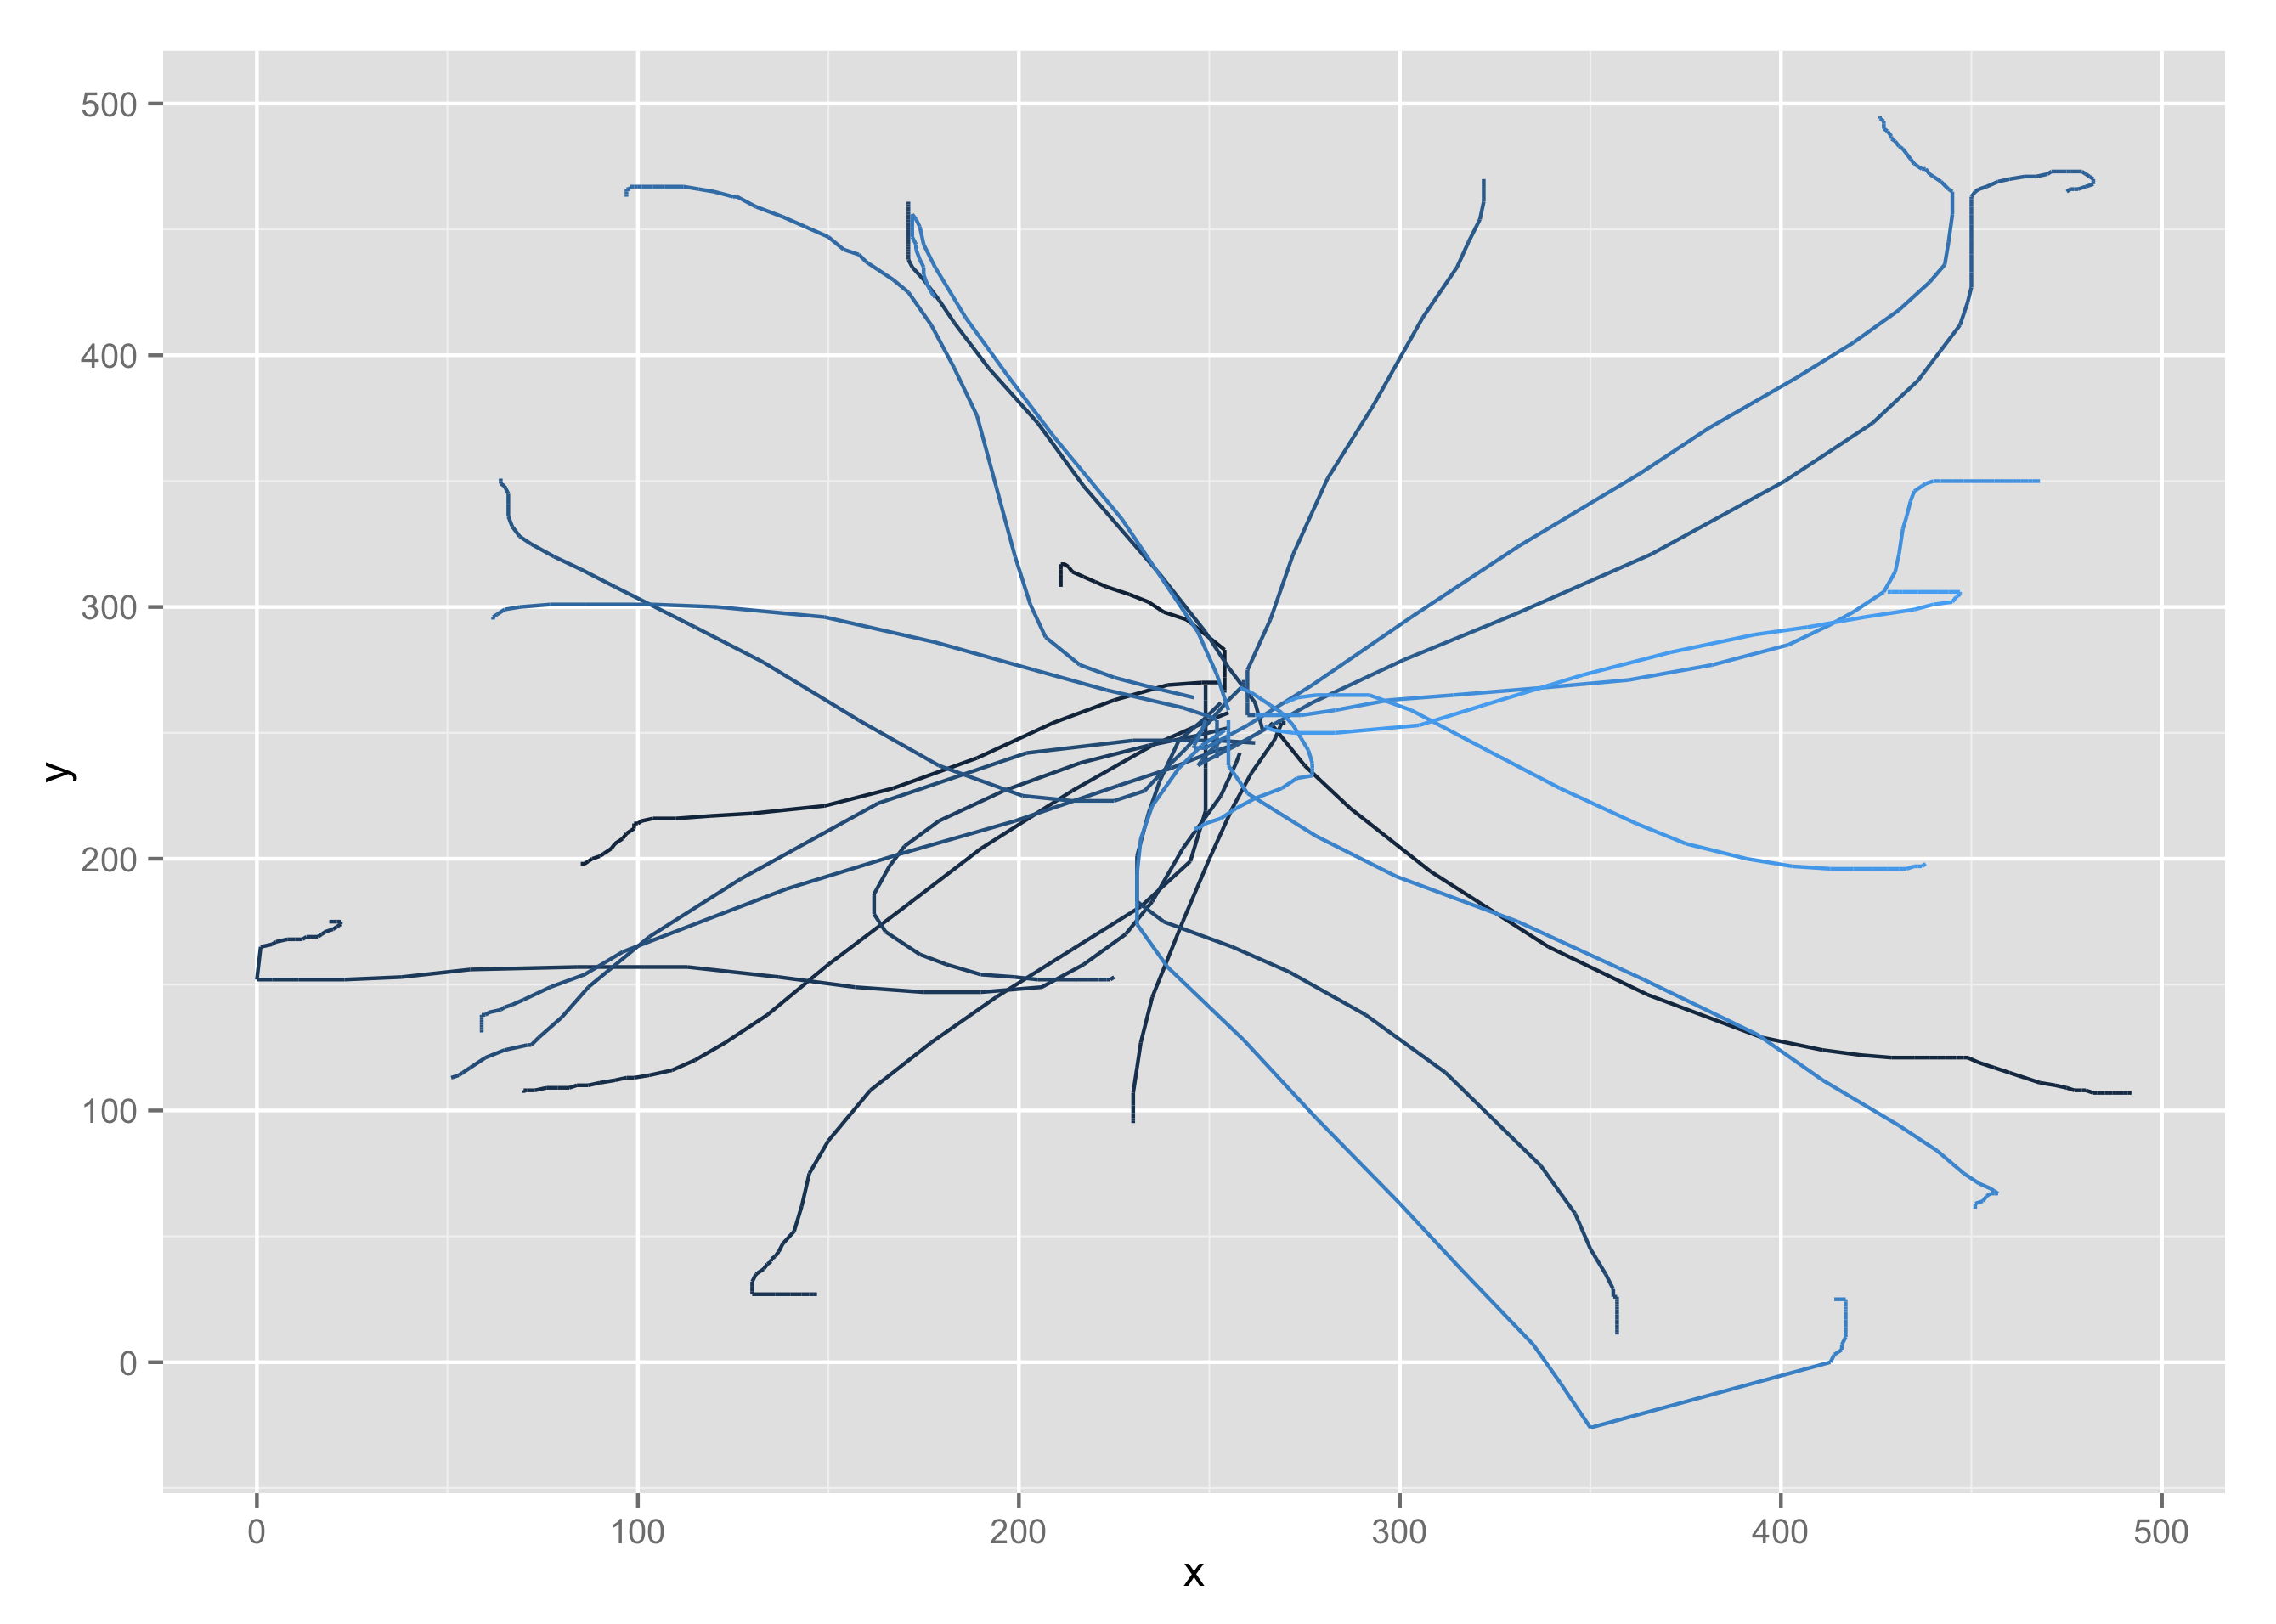
\includegraphics[width=\linewidth]{images/plots/plot_analysis_qualitative_235}
	\end{minipage}
	\begin{minipage}{0.5\linewidth}
		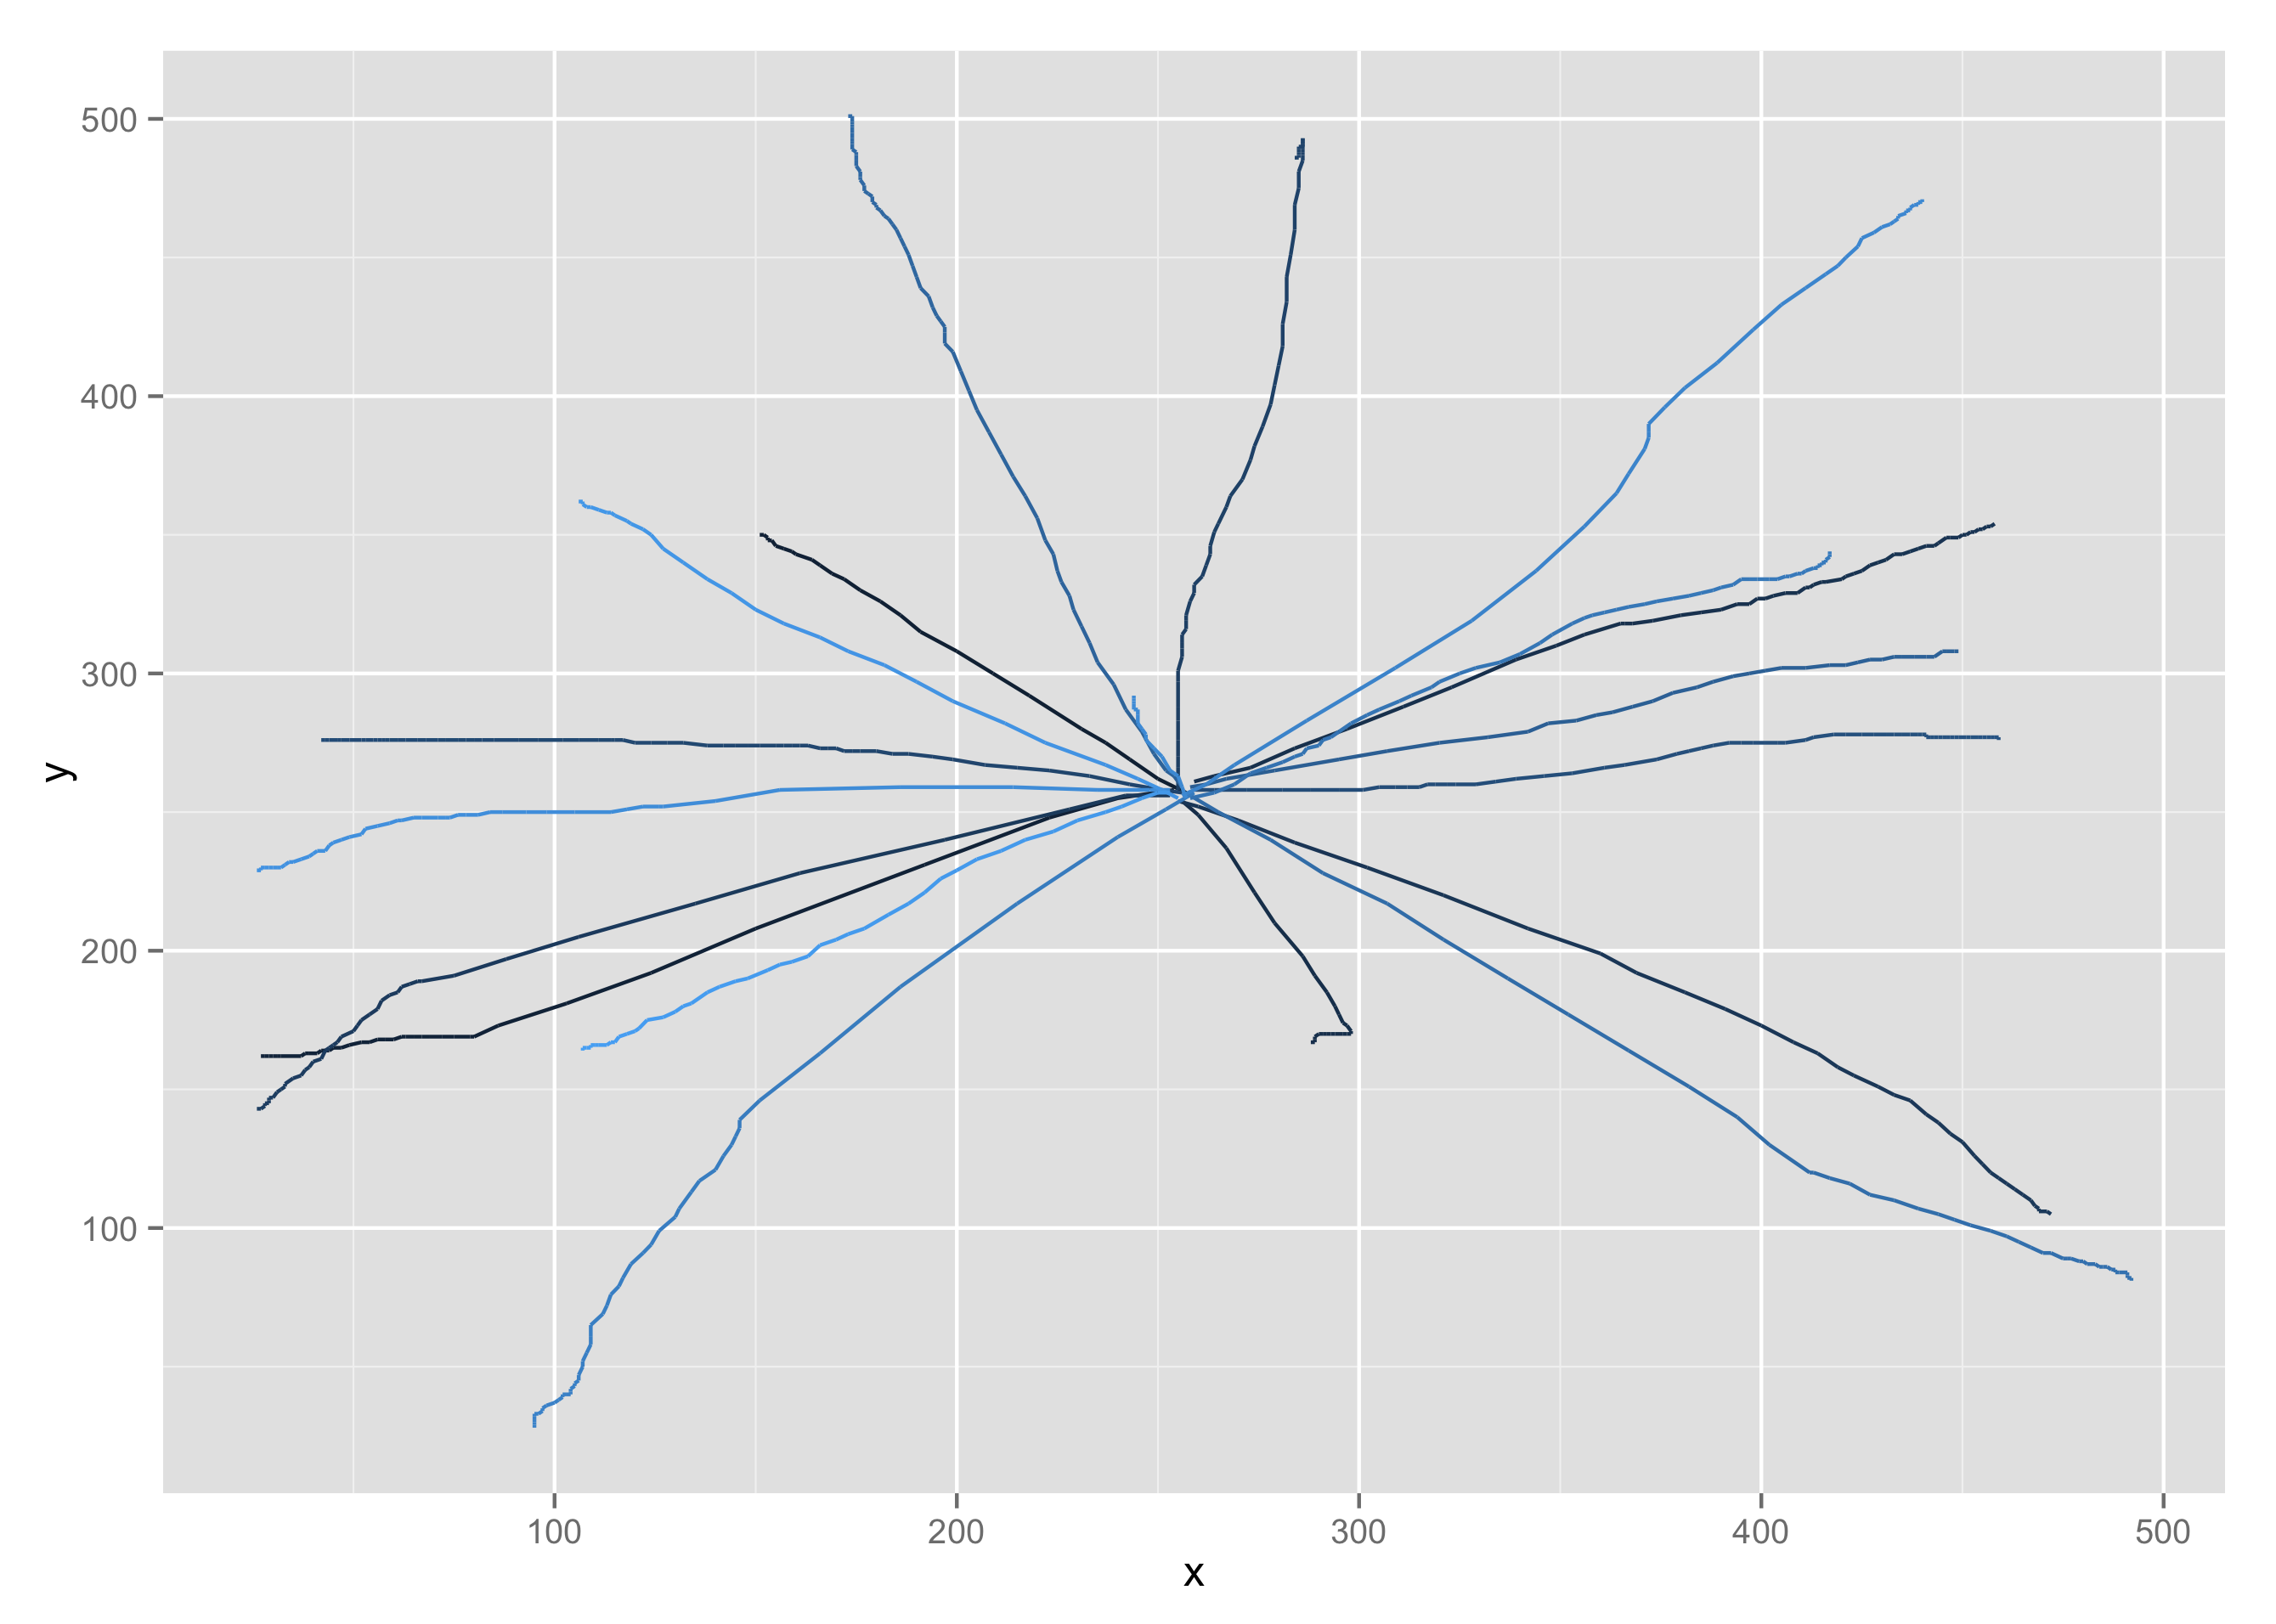
\includegraphics[width=\linewidth]{images/plots/plot_analysis_qualitative_239}
	\end{minipage}	
	\captionof{figure}{6 testdeltageres bevægelsesbaner for de 25 pegeopgaver}
	\label{fig:kvaliativ_persons_1}
\end{minipage}

\begin{minipage}{\textwidth}
	\begin{minipage}{0.5\linewidth}
		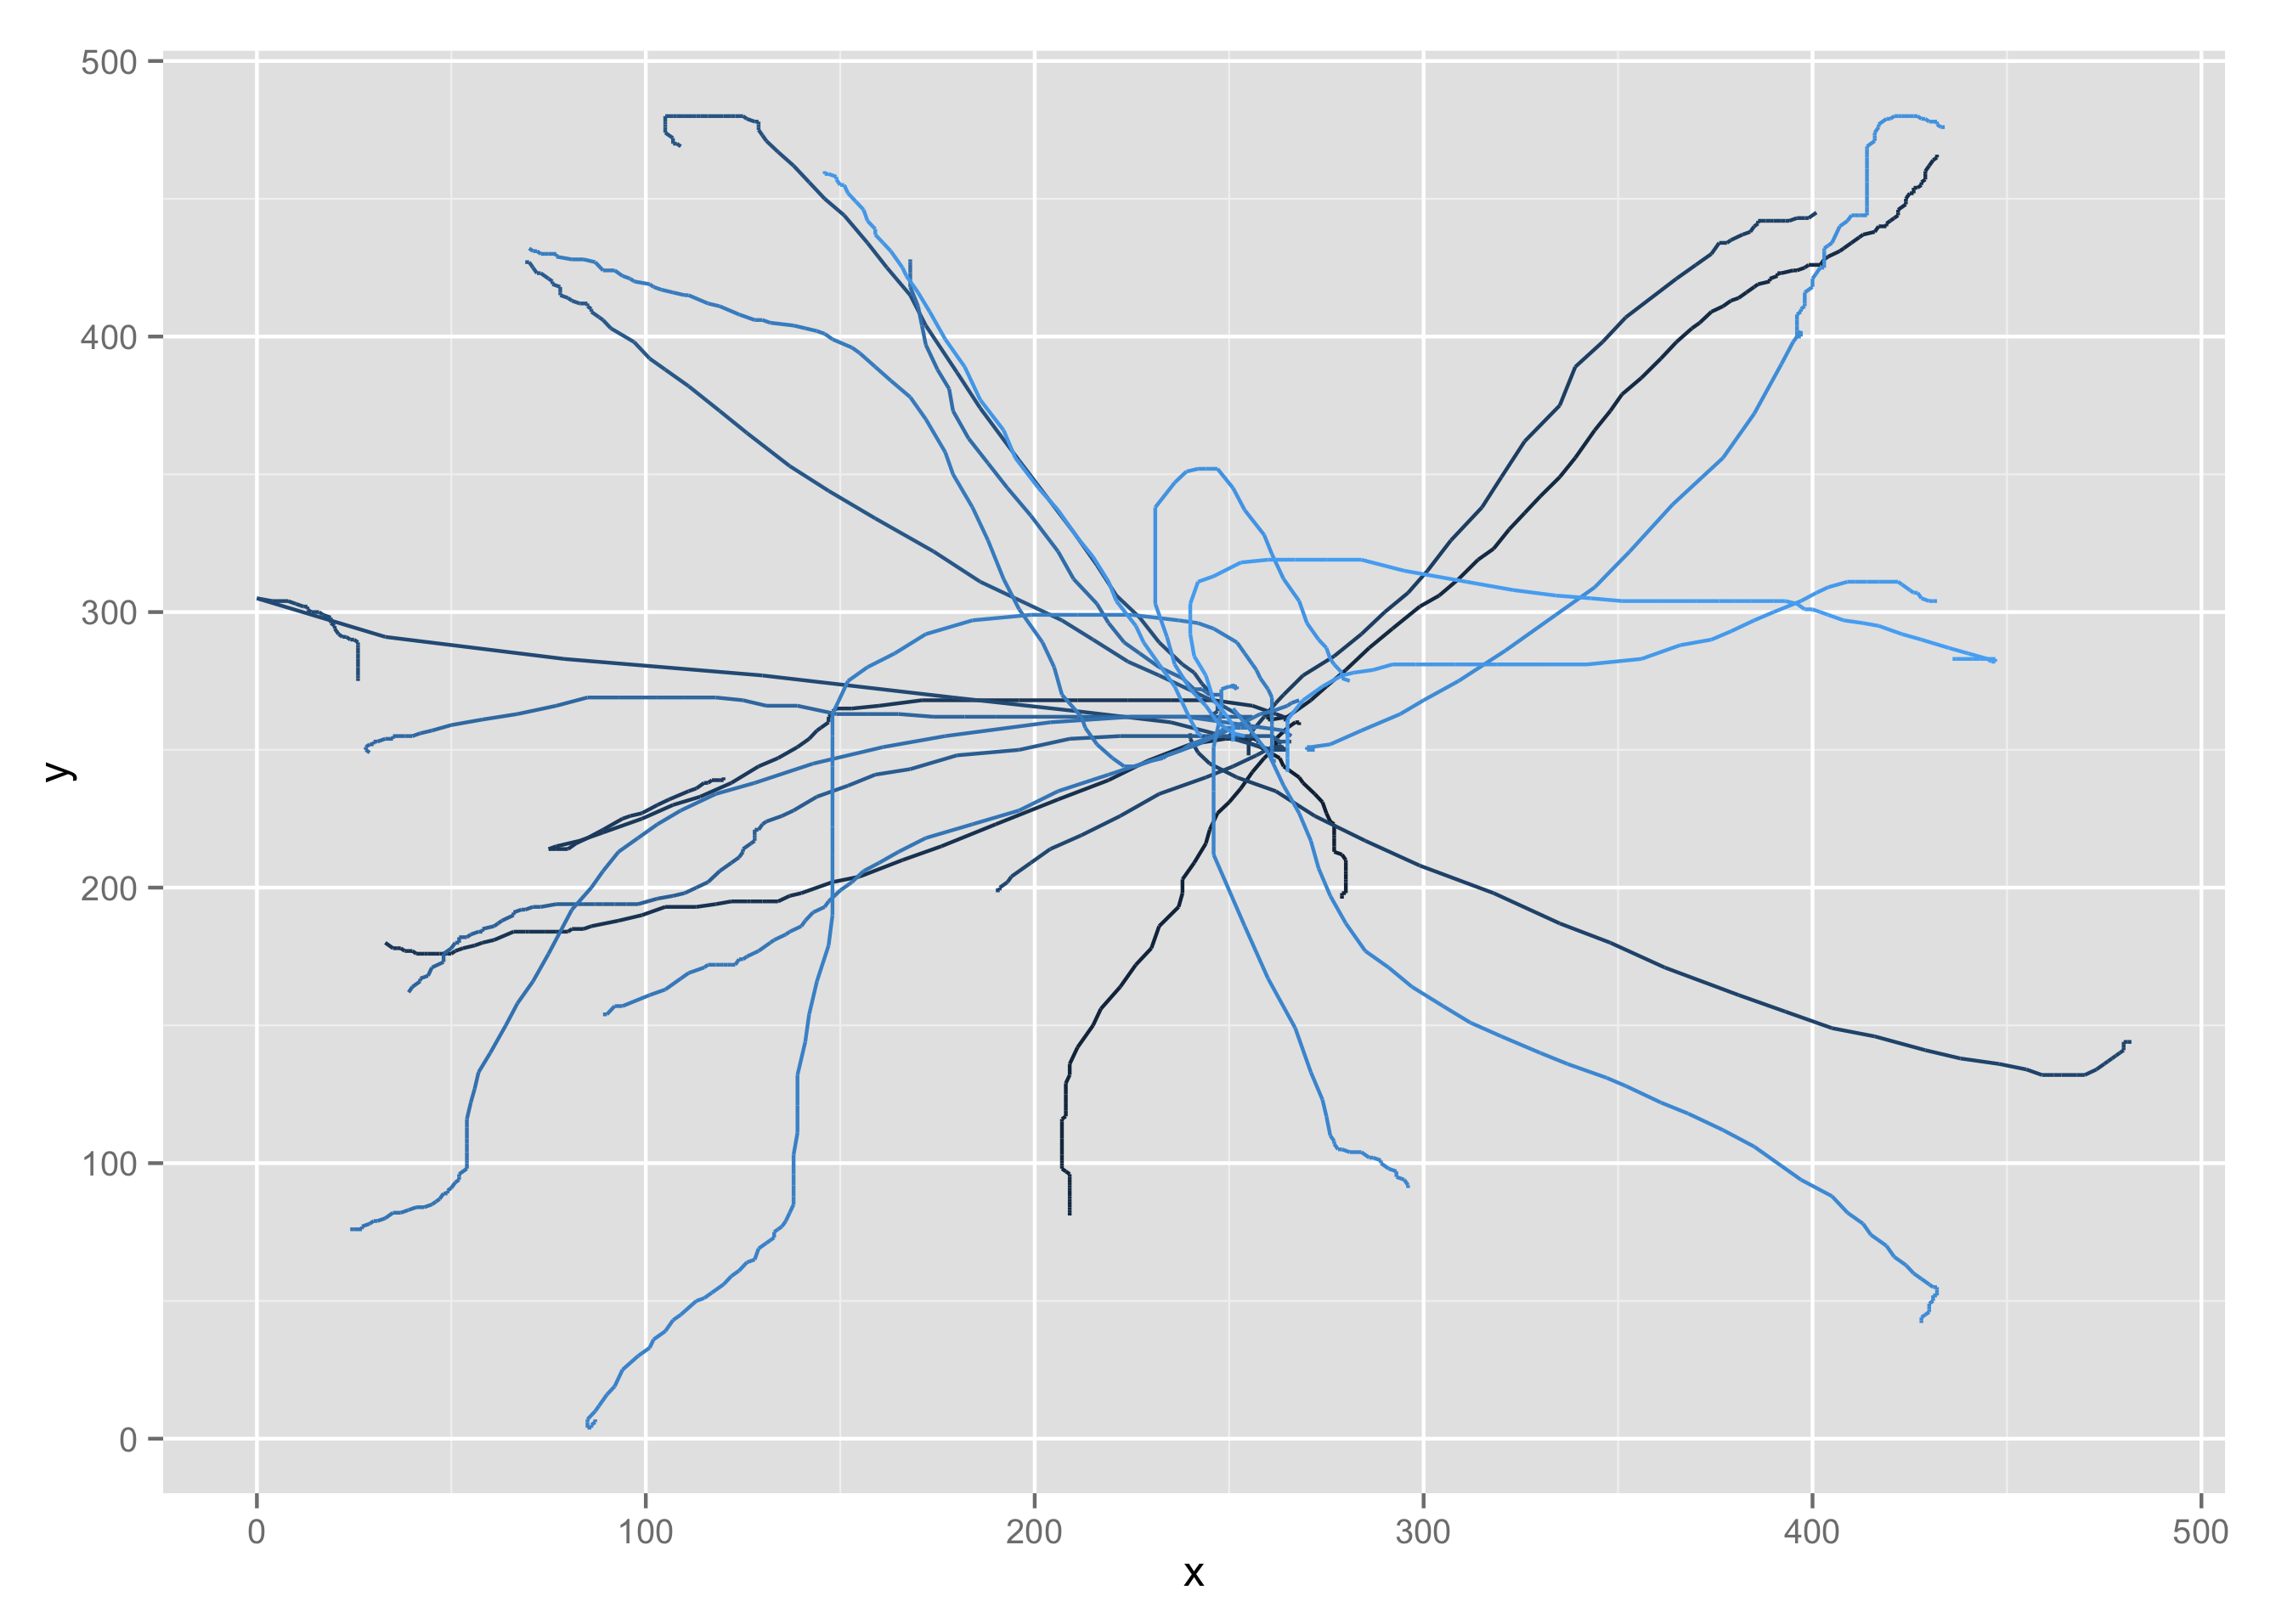
\includegraphics[width=\linewidth]{images/plots/plot_analysis_qualitative_113}
	\end{minipage}
	\begin{minipage}{0.5\linewidth}
		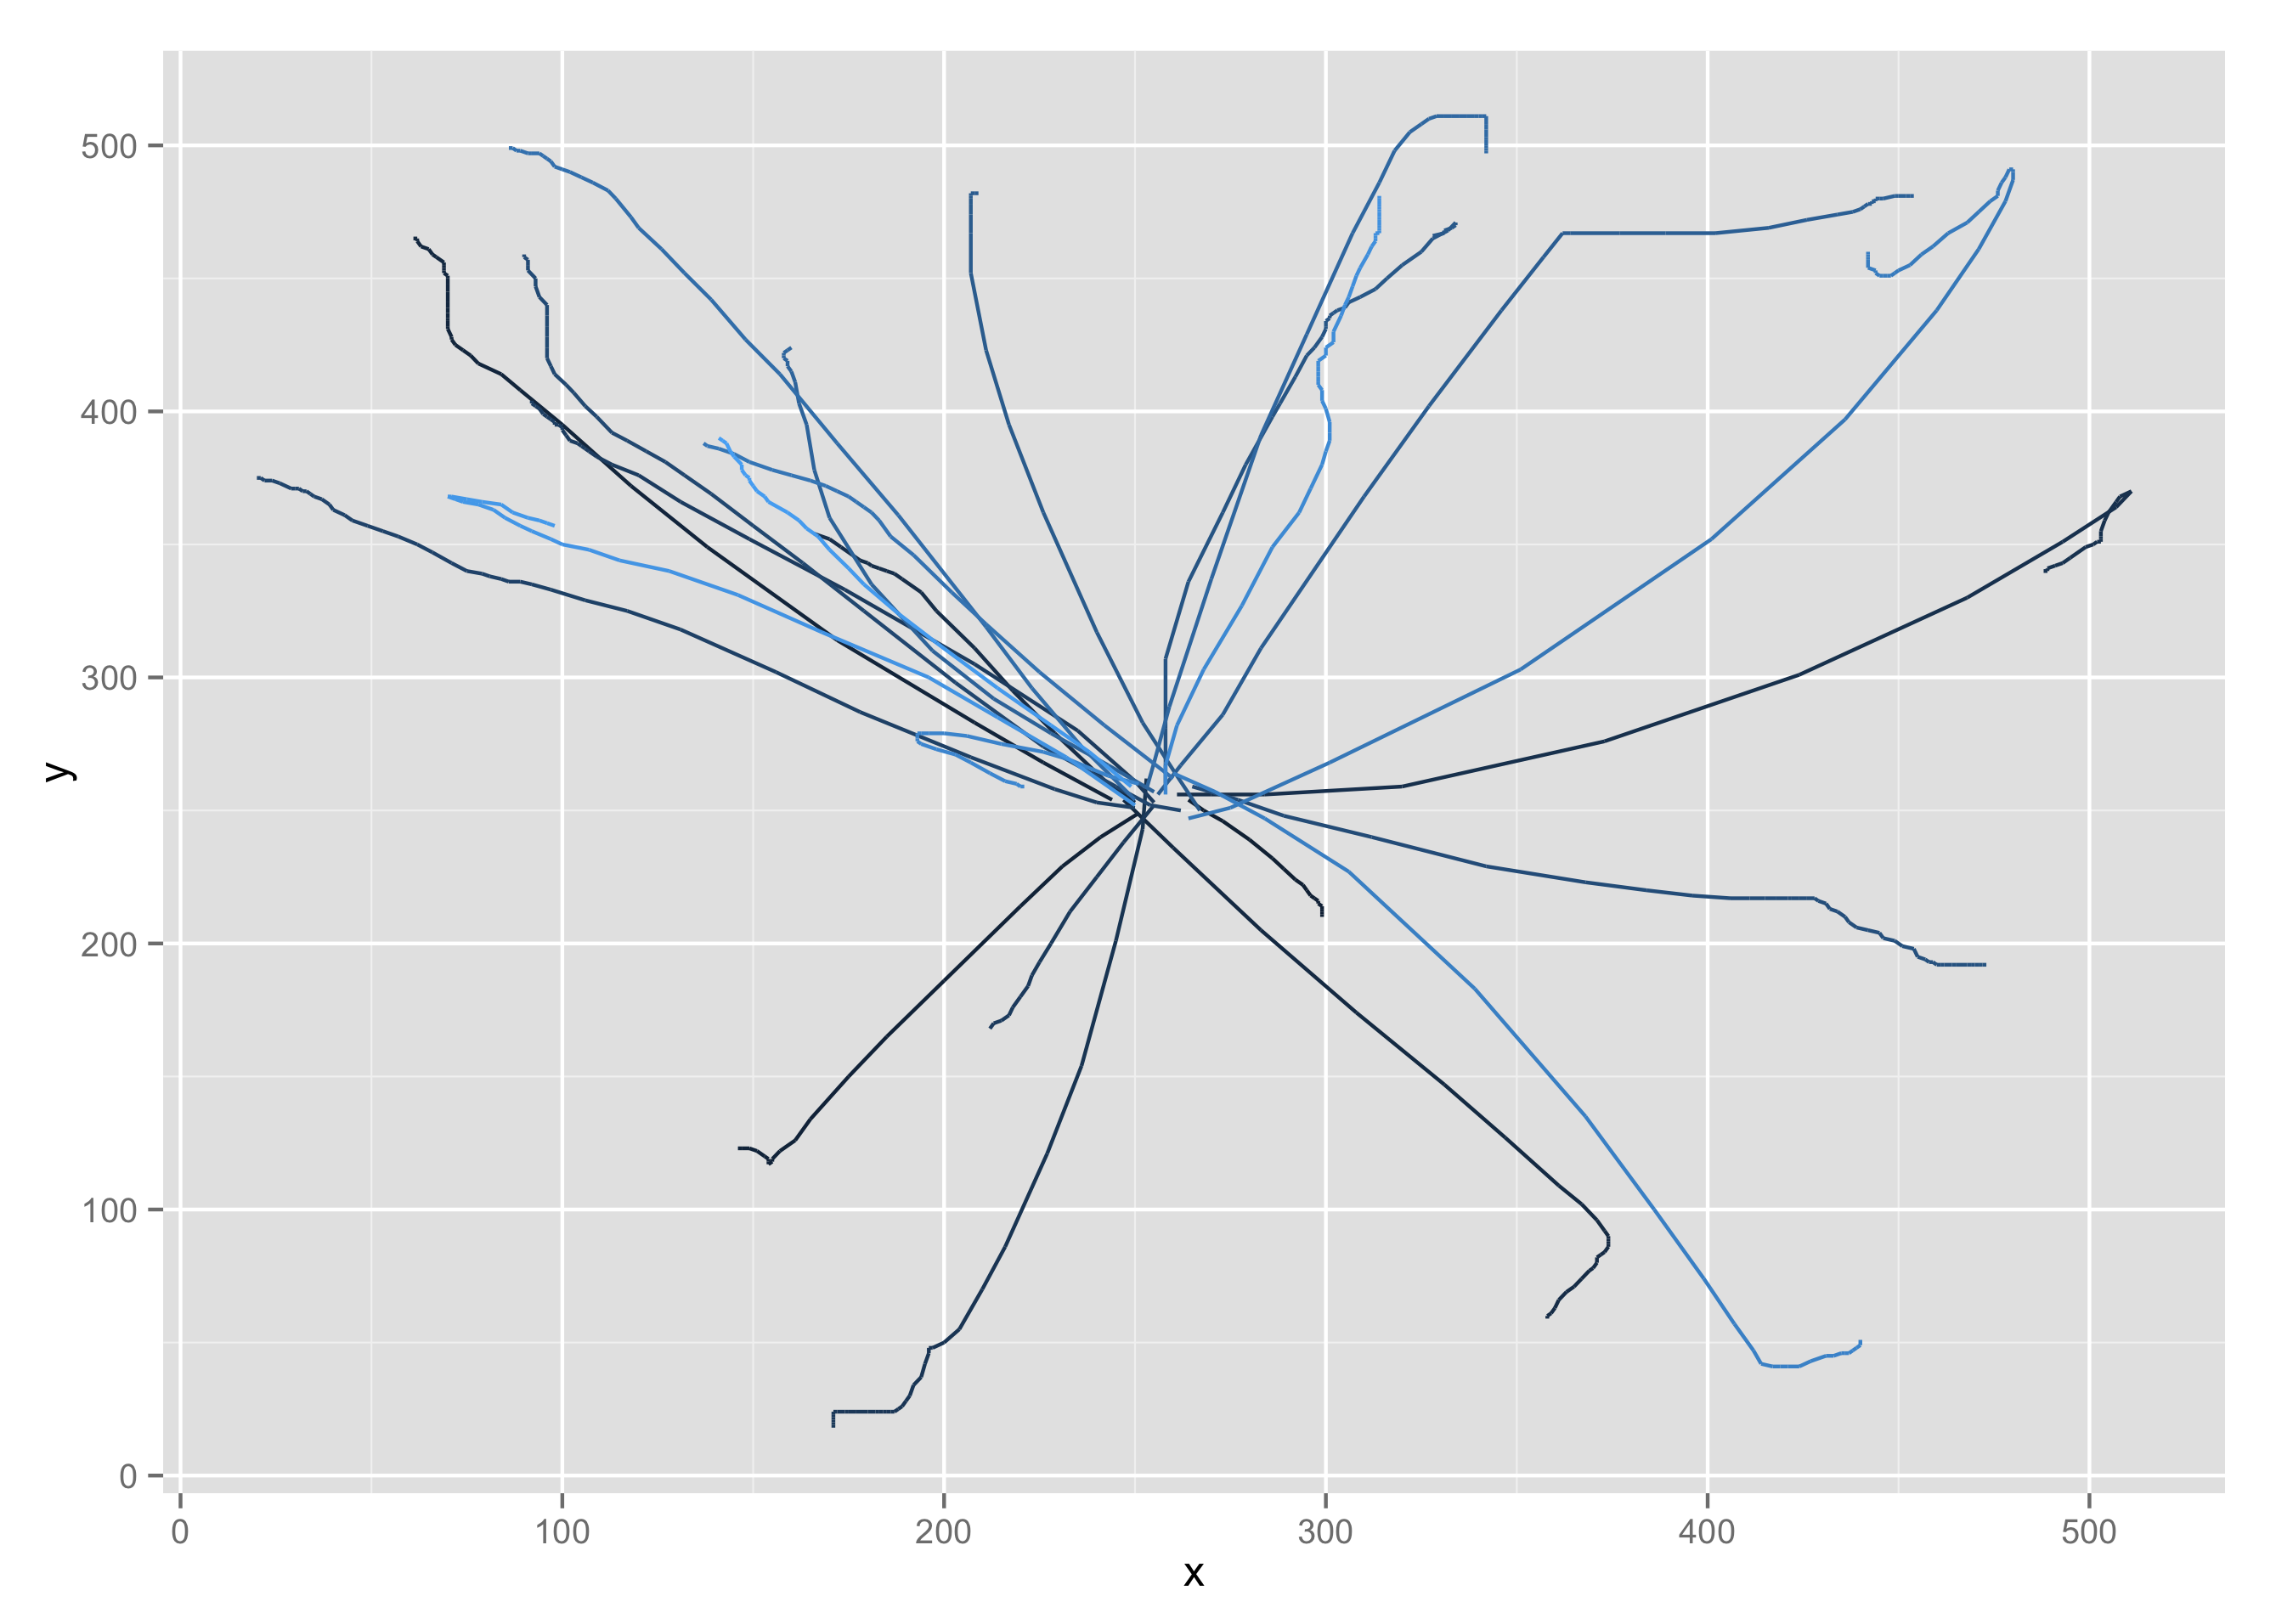
\includegraphics[width=\linewidth]{images/plots/plot_analysis_qualitative_263}
	\end{minipage}
	\begin{minipage}{0.5\linewidth}
		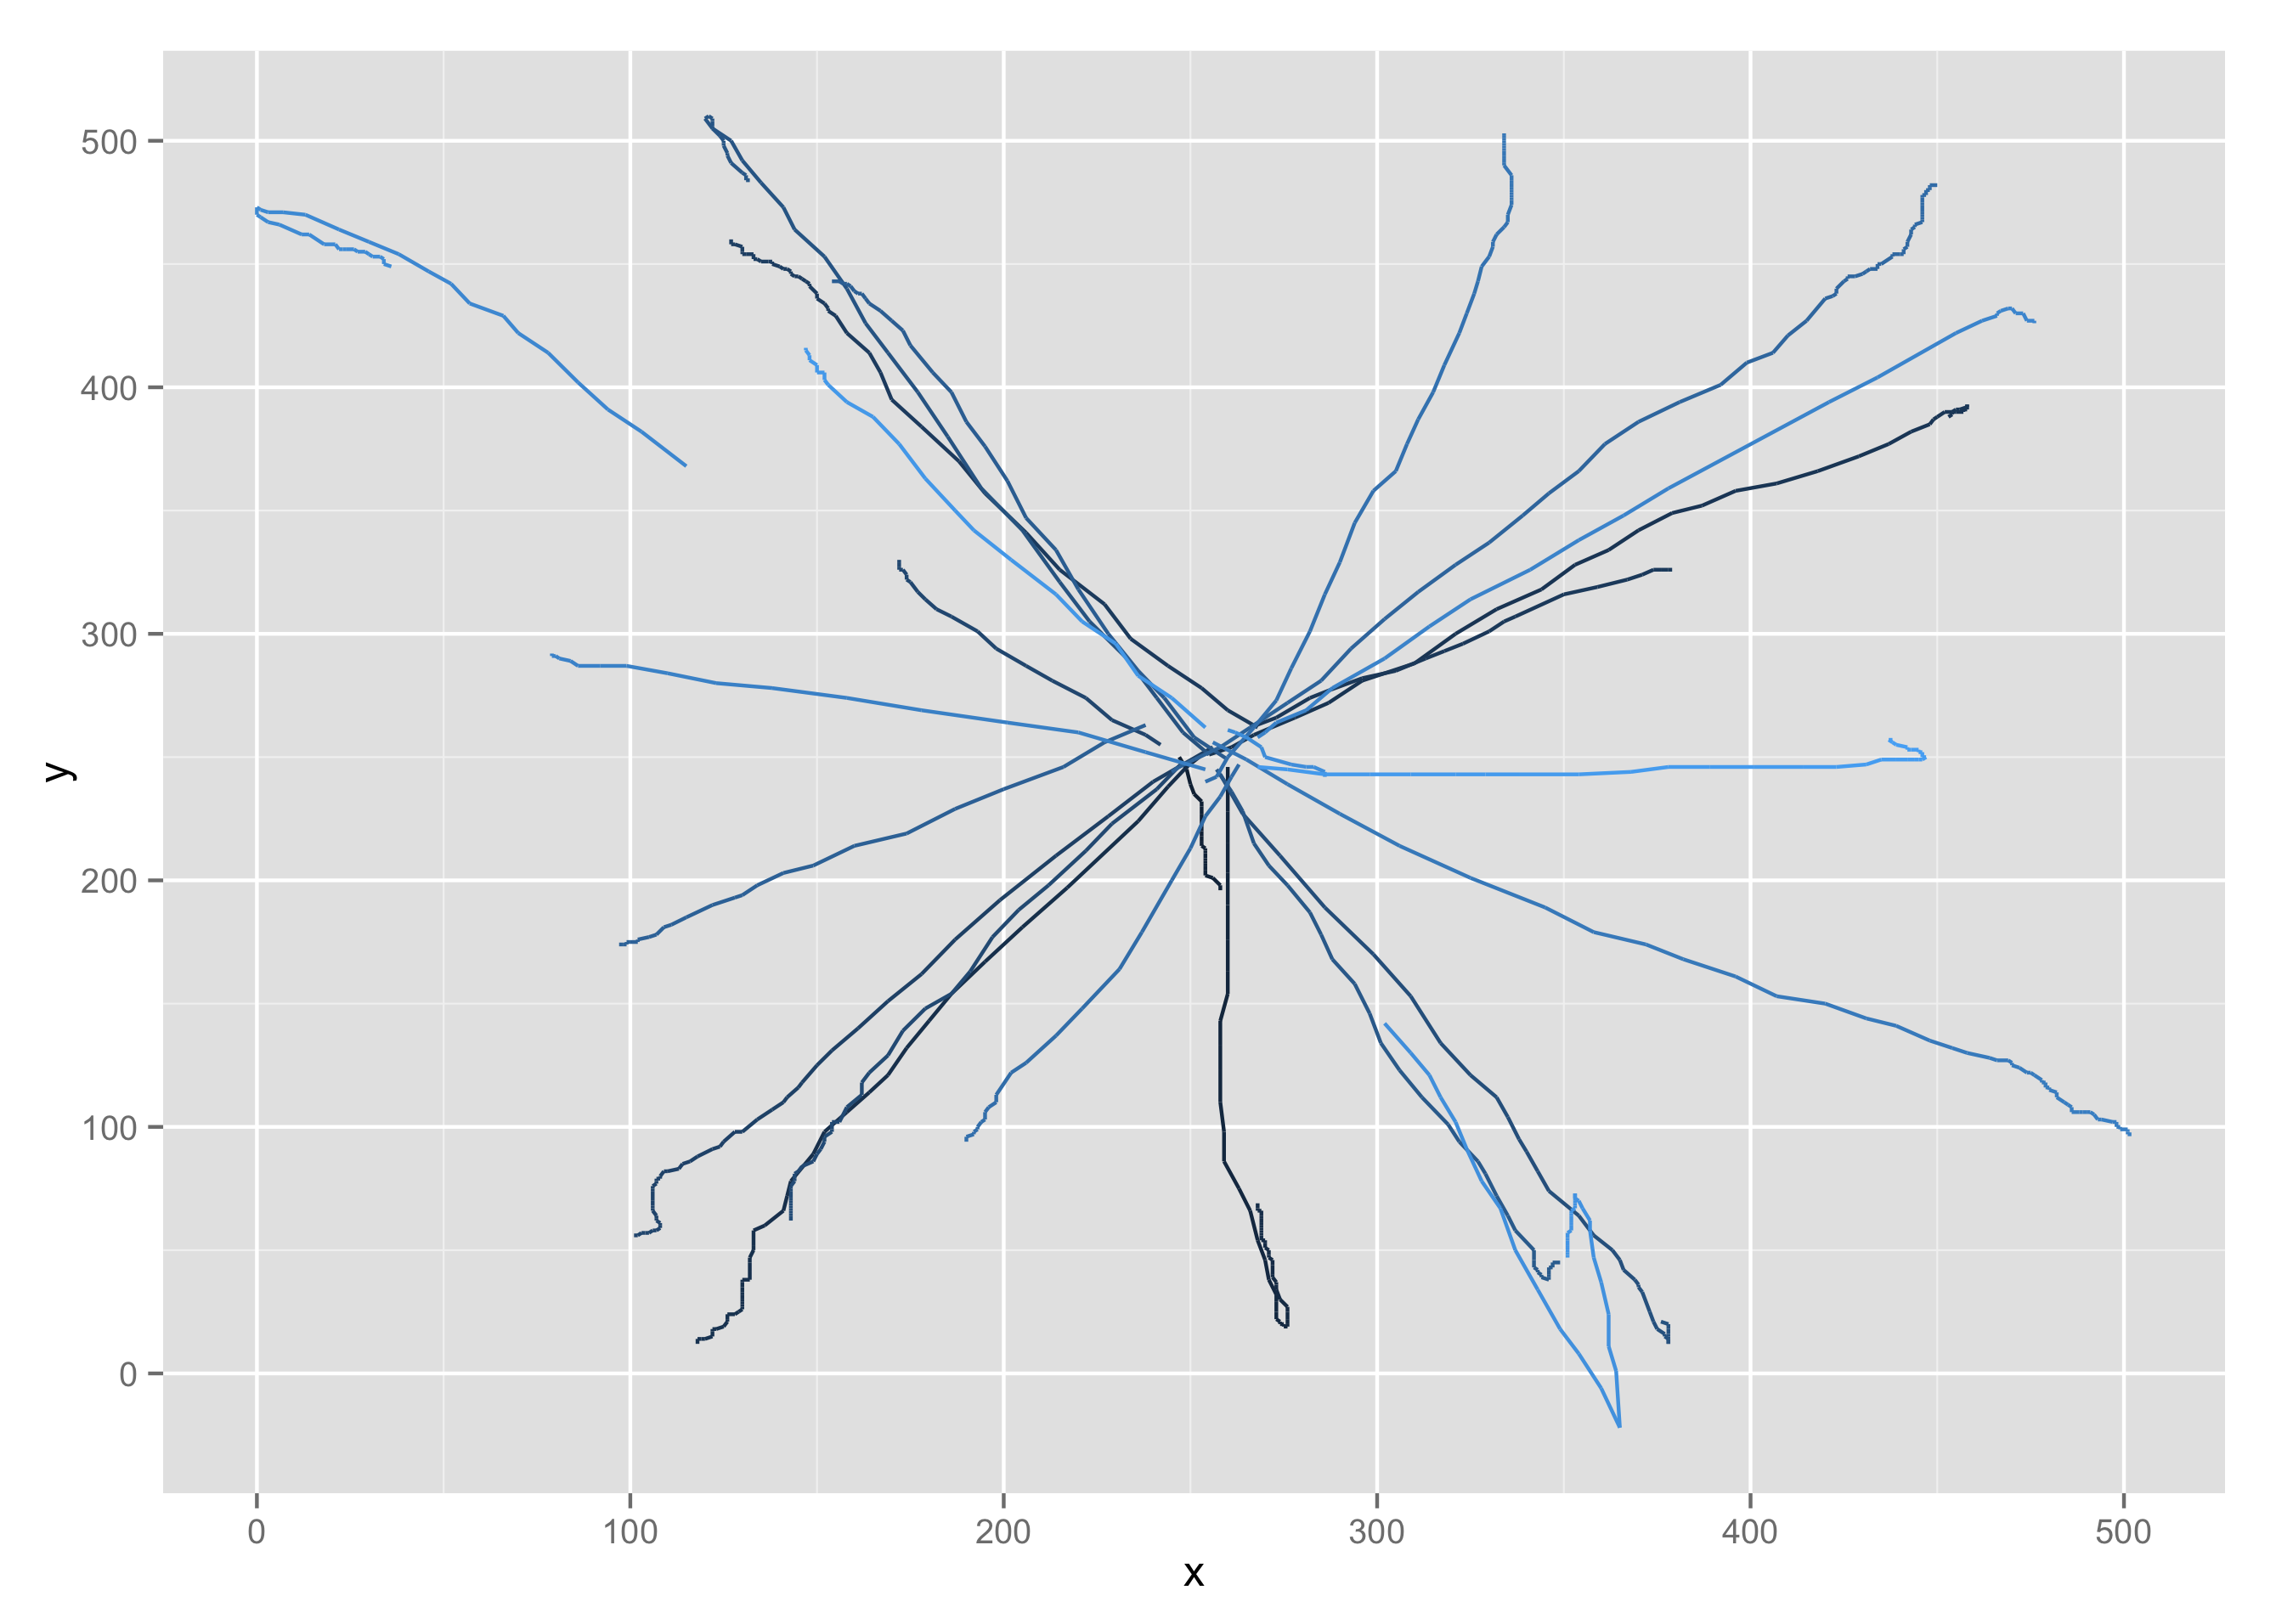
\includegraphics[width=\linewidth]{images/plots/plot_analysis_qualitative_166}
	\end{minipage}
		\begin{minipage}{0.5\linewidth}
		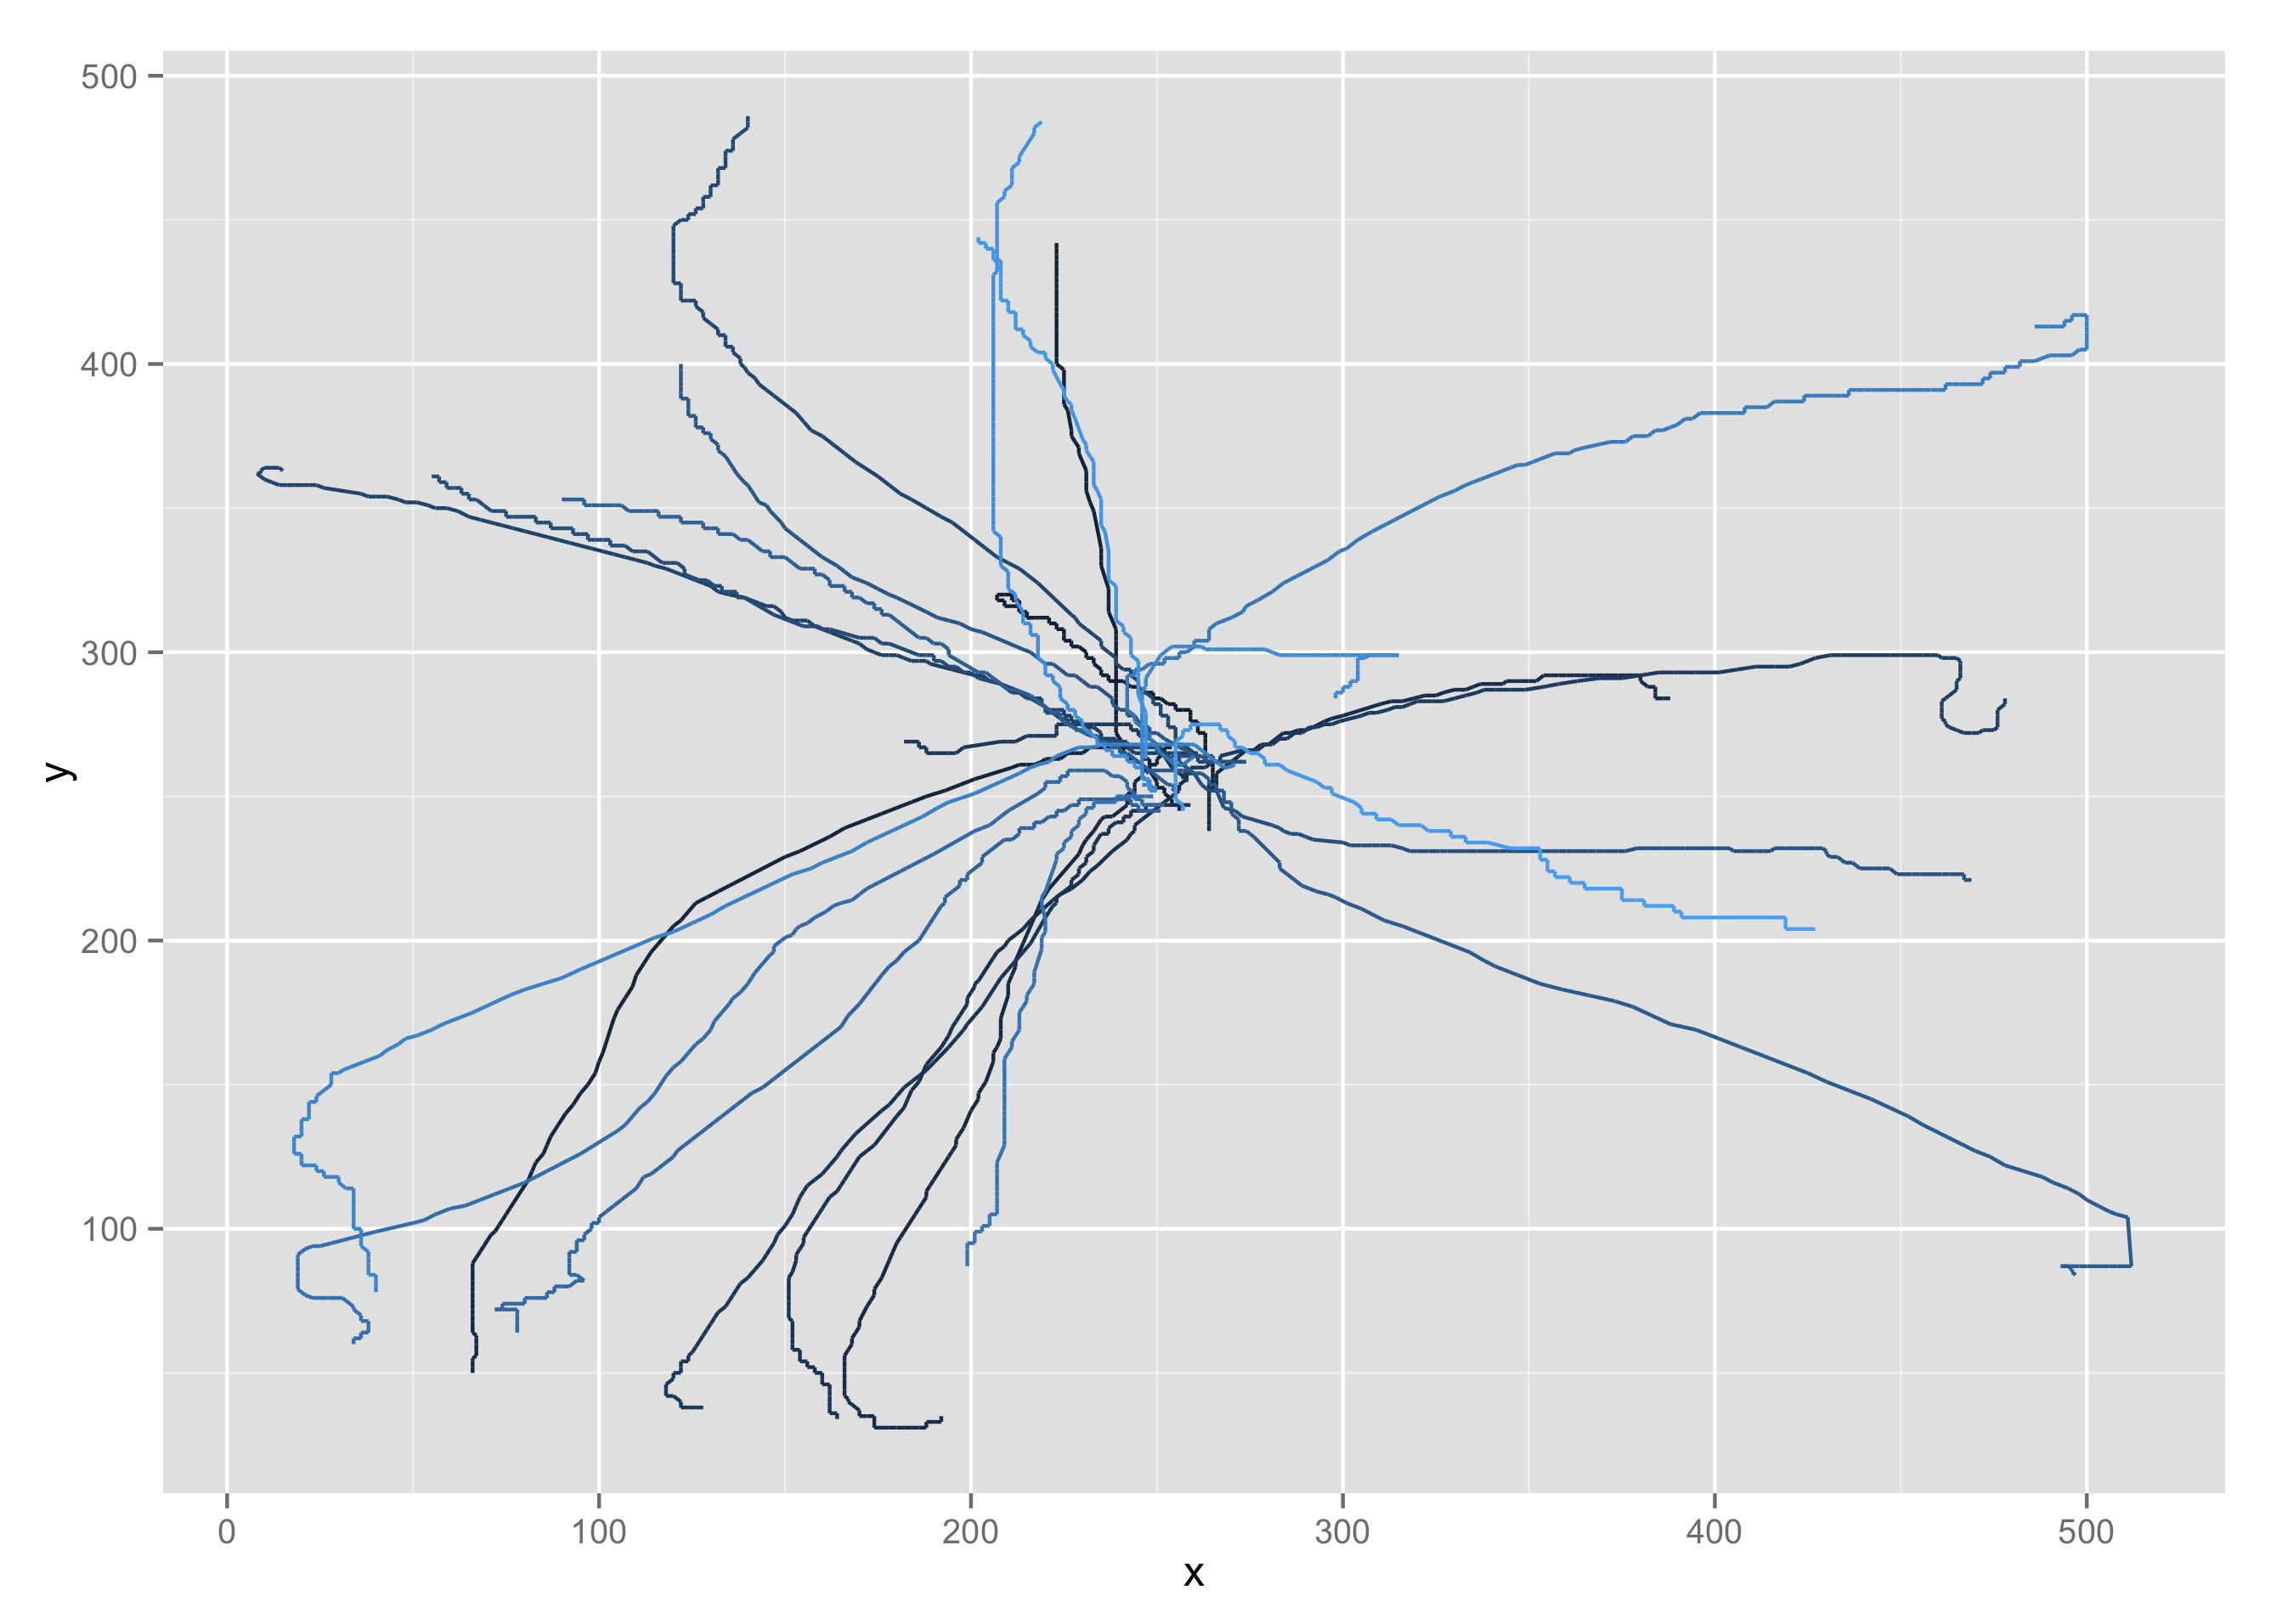
\includegraphics[width=\linewidth]{images/plots/plot_analysis_qualitative_72}
	\end{minipage}
	\begin{minipage}{0.5\linewidth}
		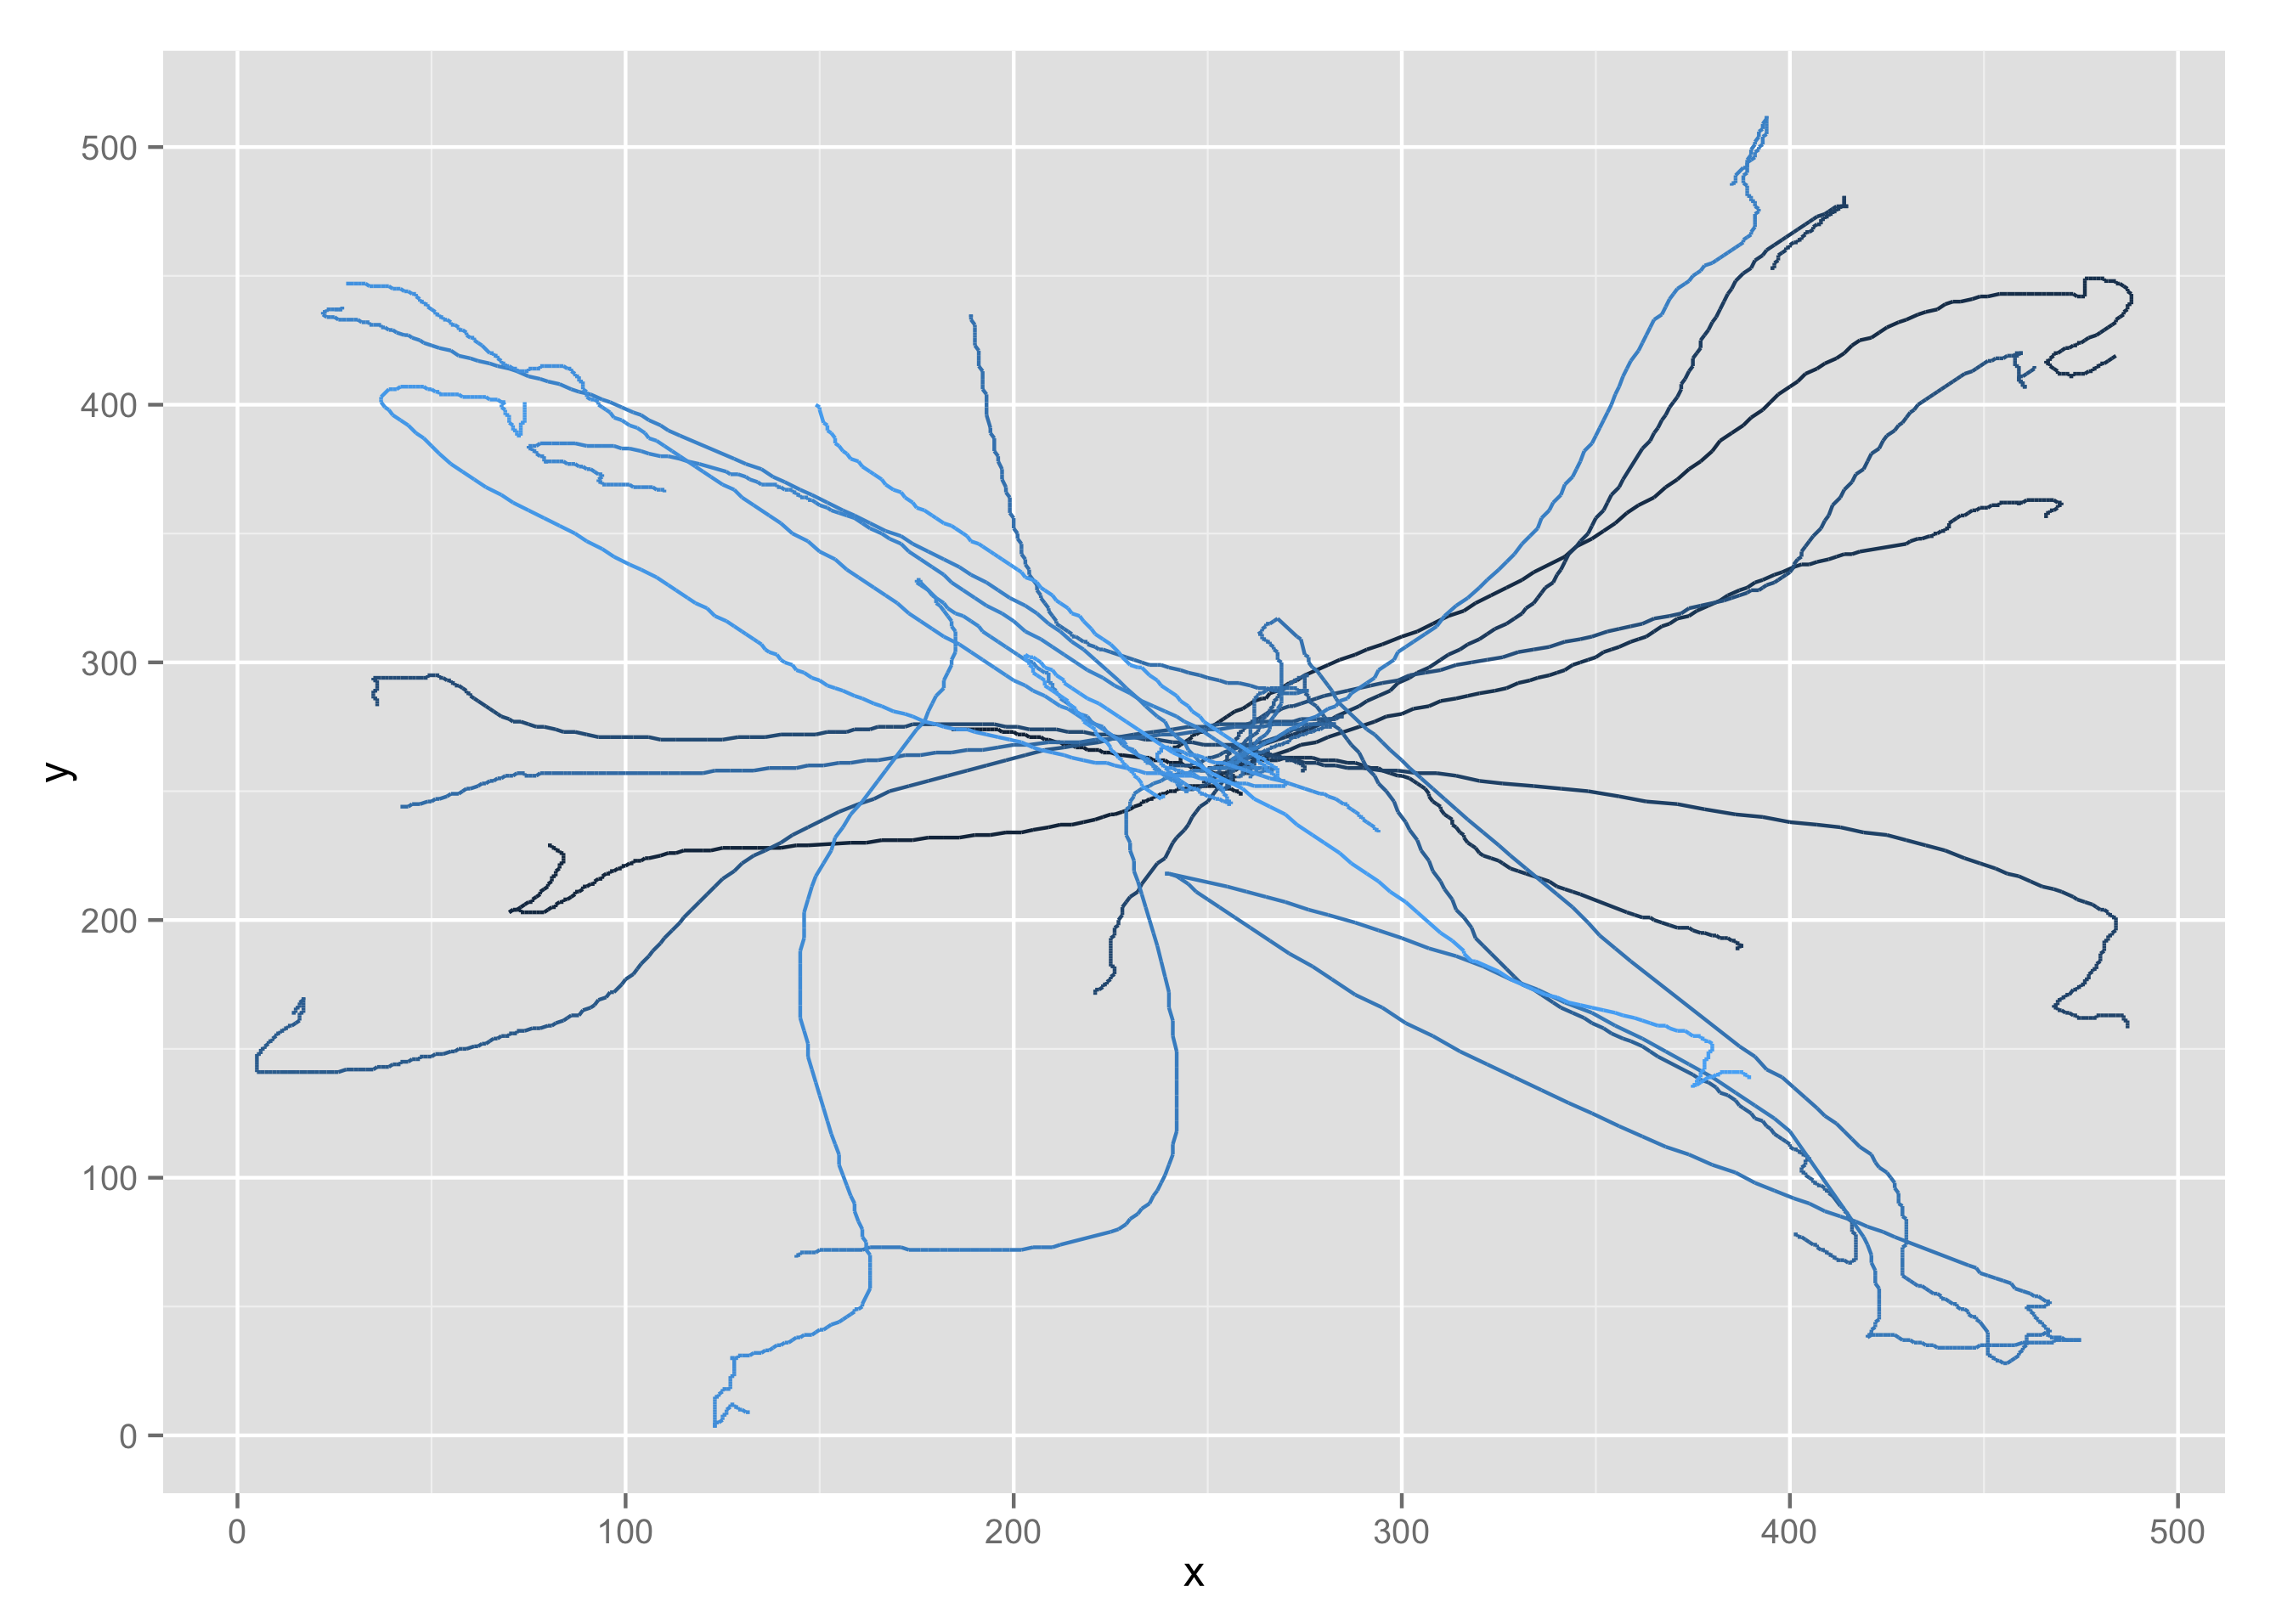
\includegraphics[width=\linewidth]{images/plots/plot_analysis_qualitative_151}
	\end{minipage}
	\begin{minipage}{0.5\linewidth}
		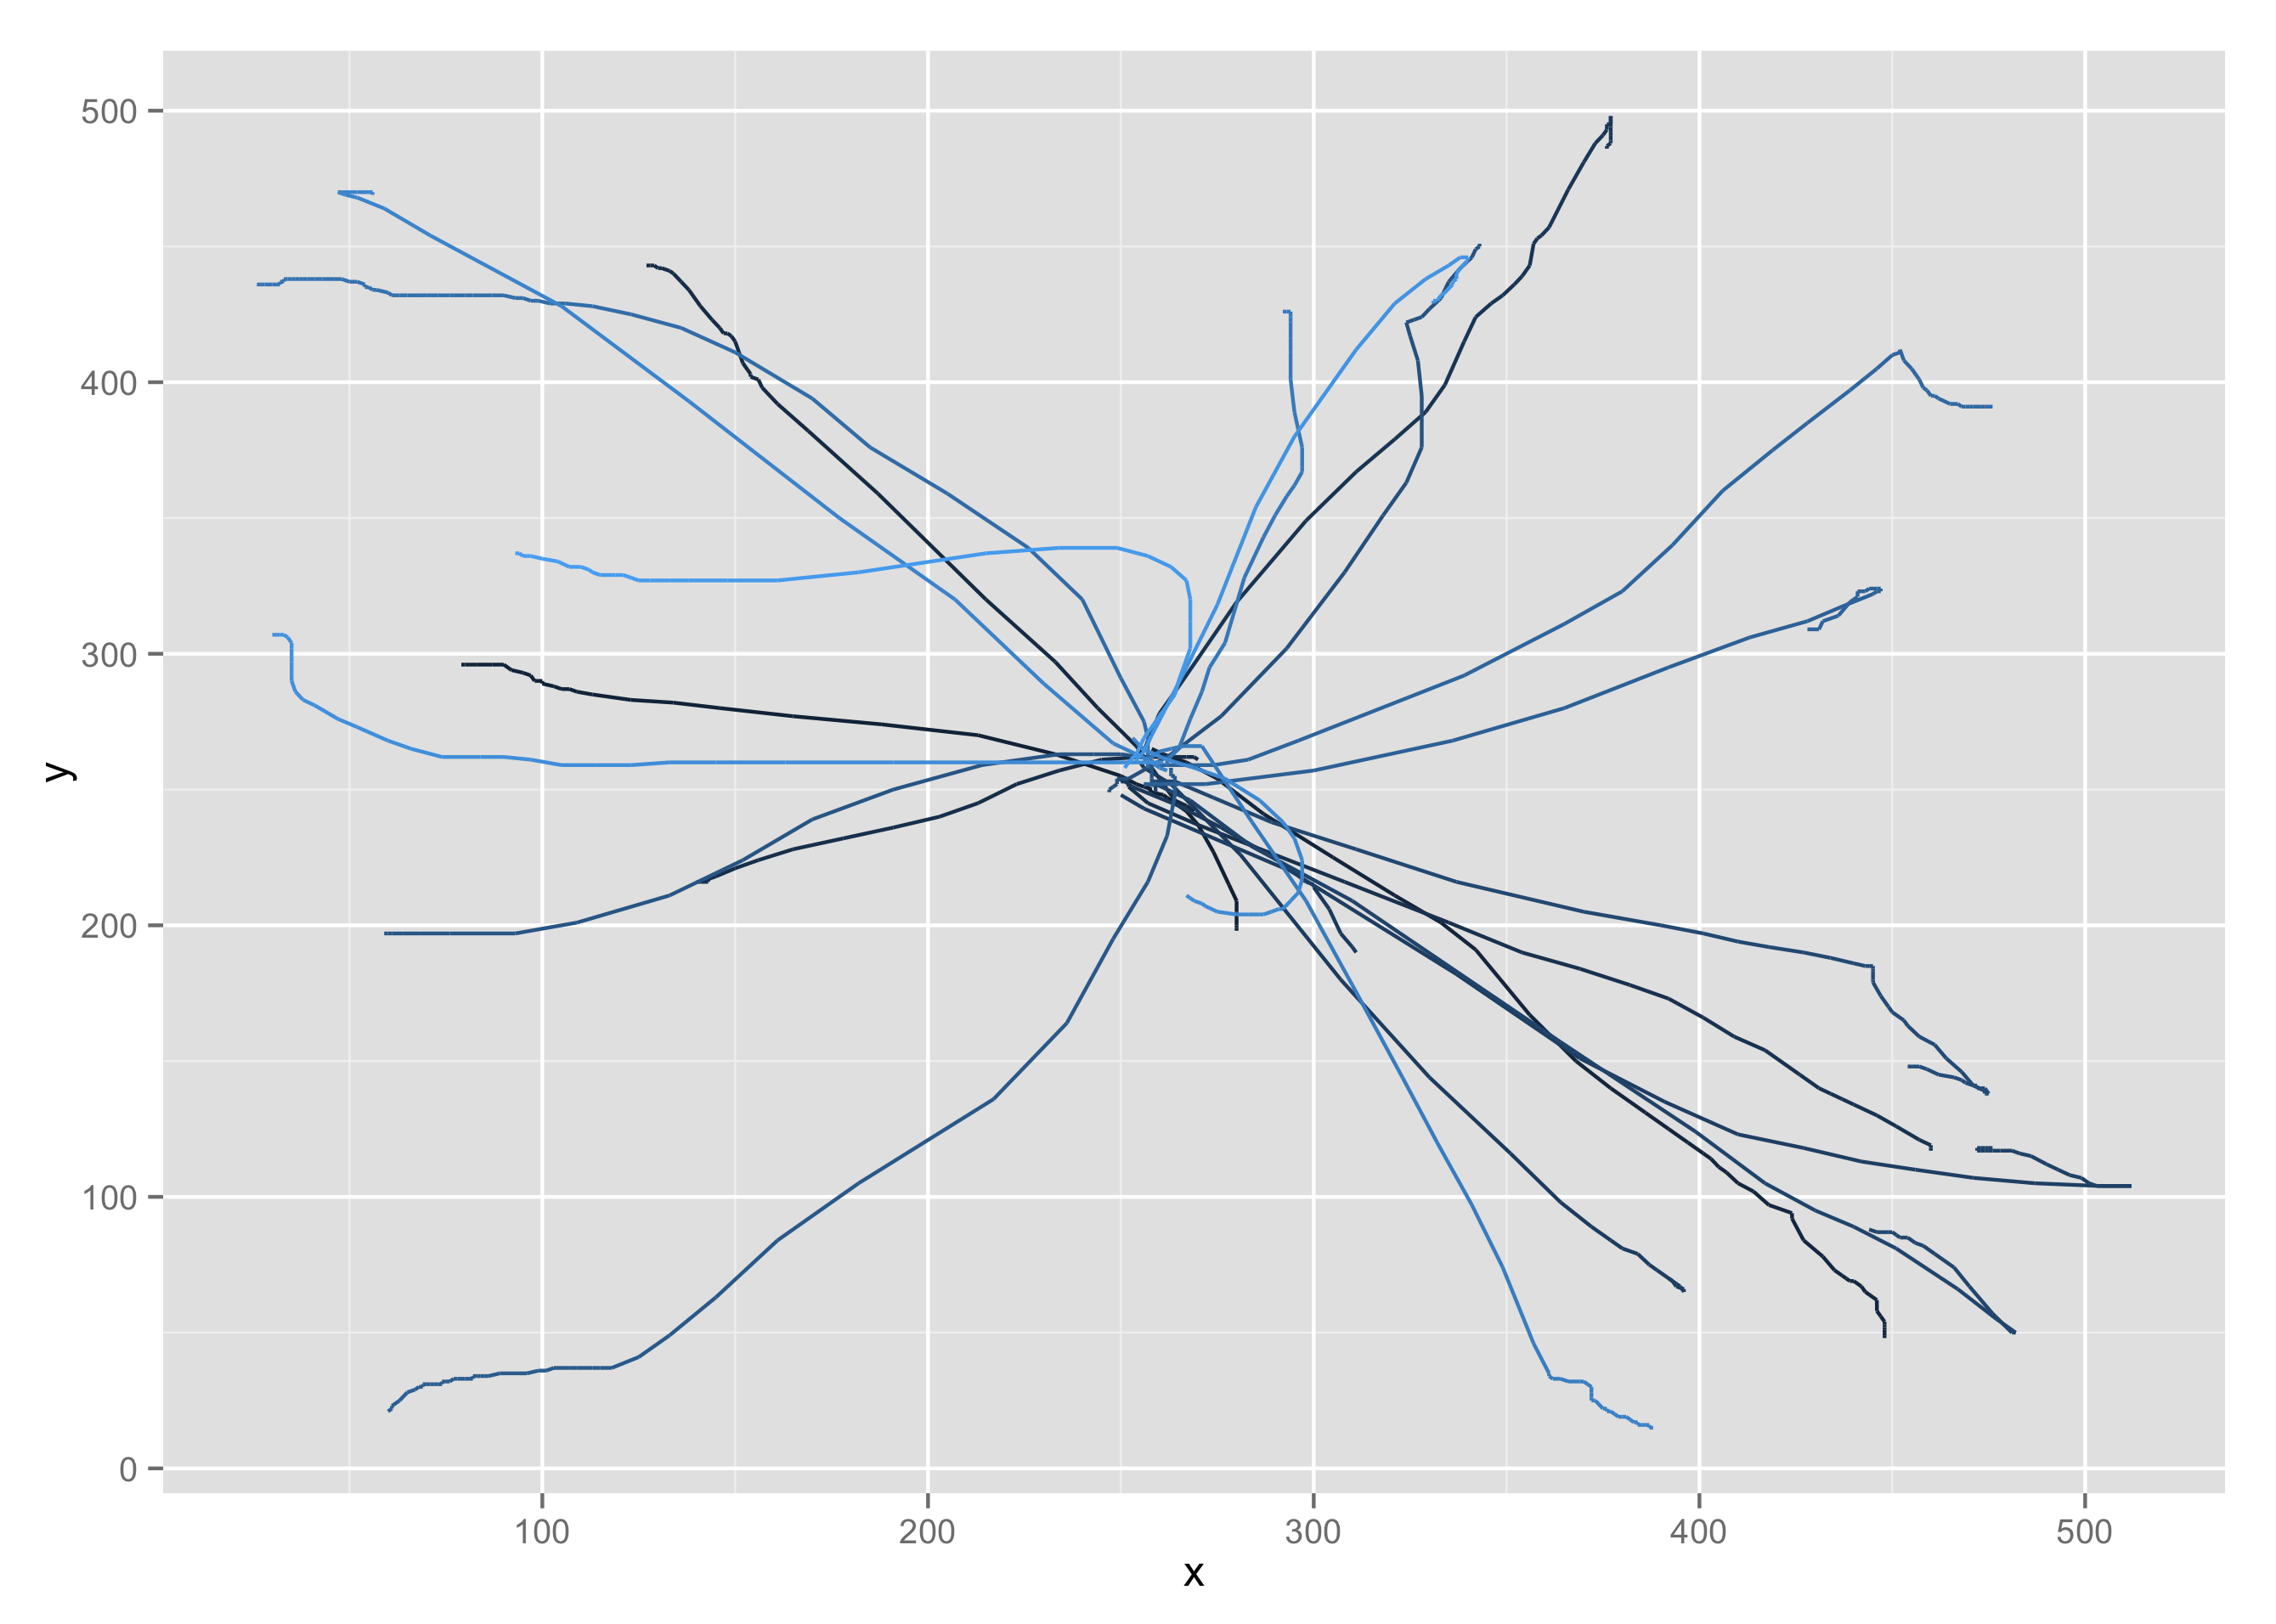
\includegraphics[width=\linewidth]{images/plots/plot_analysis_qualitative_170}
	\end{minipage}
	\begin{minipage}{0.5\linewidth}
		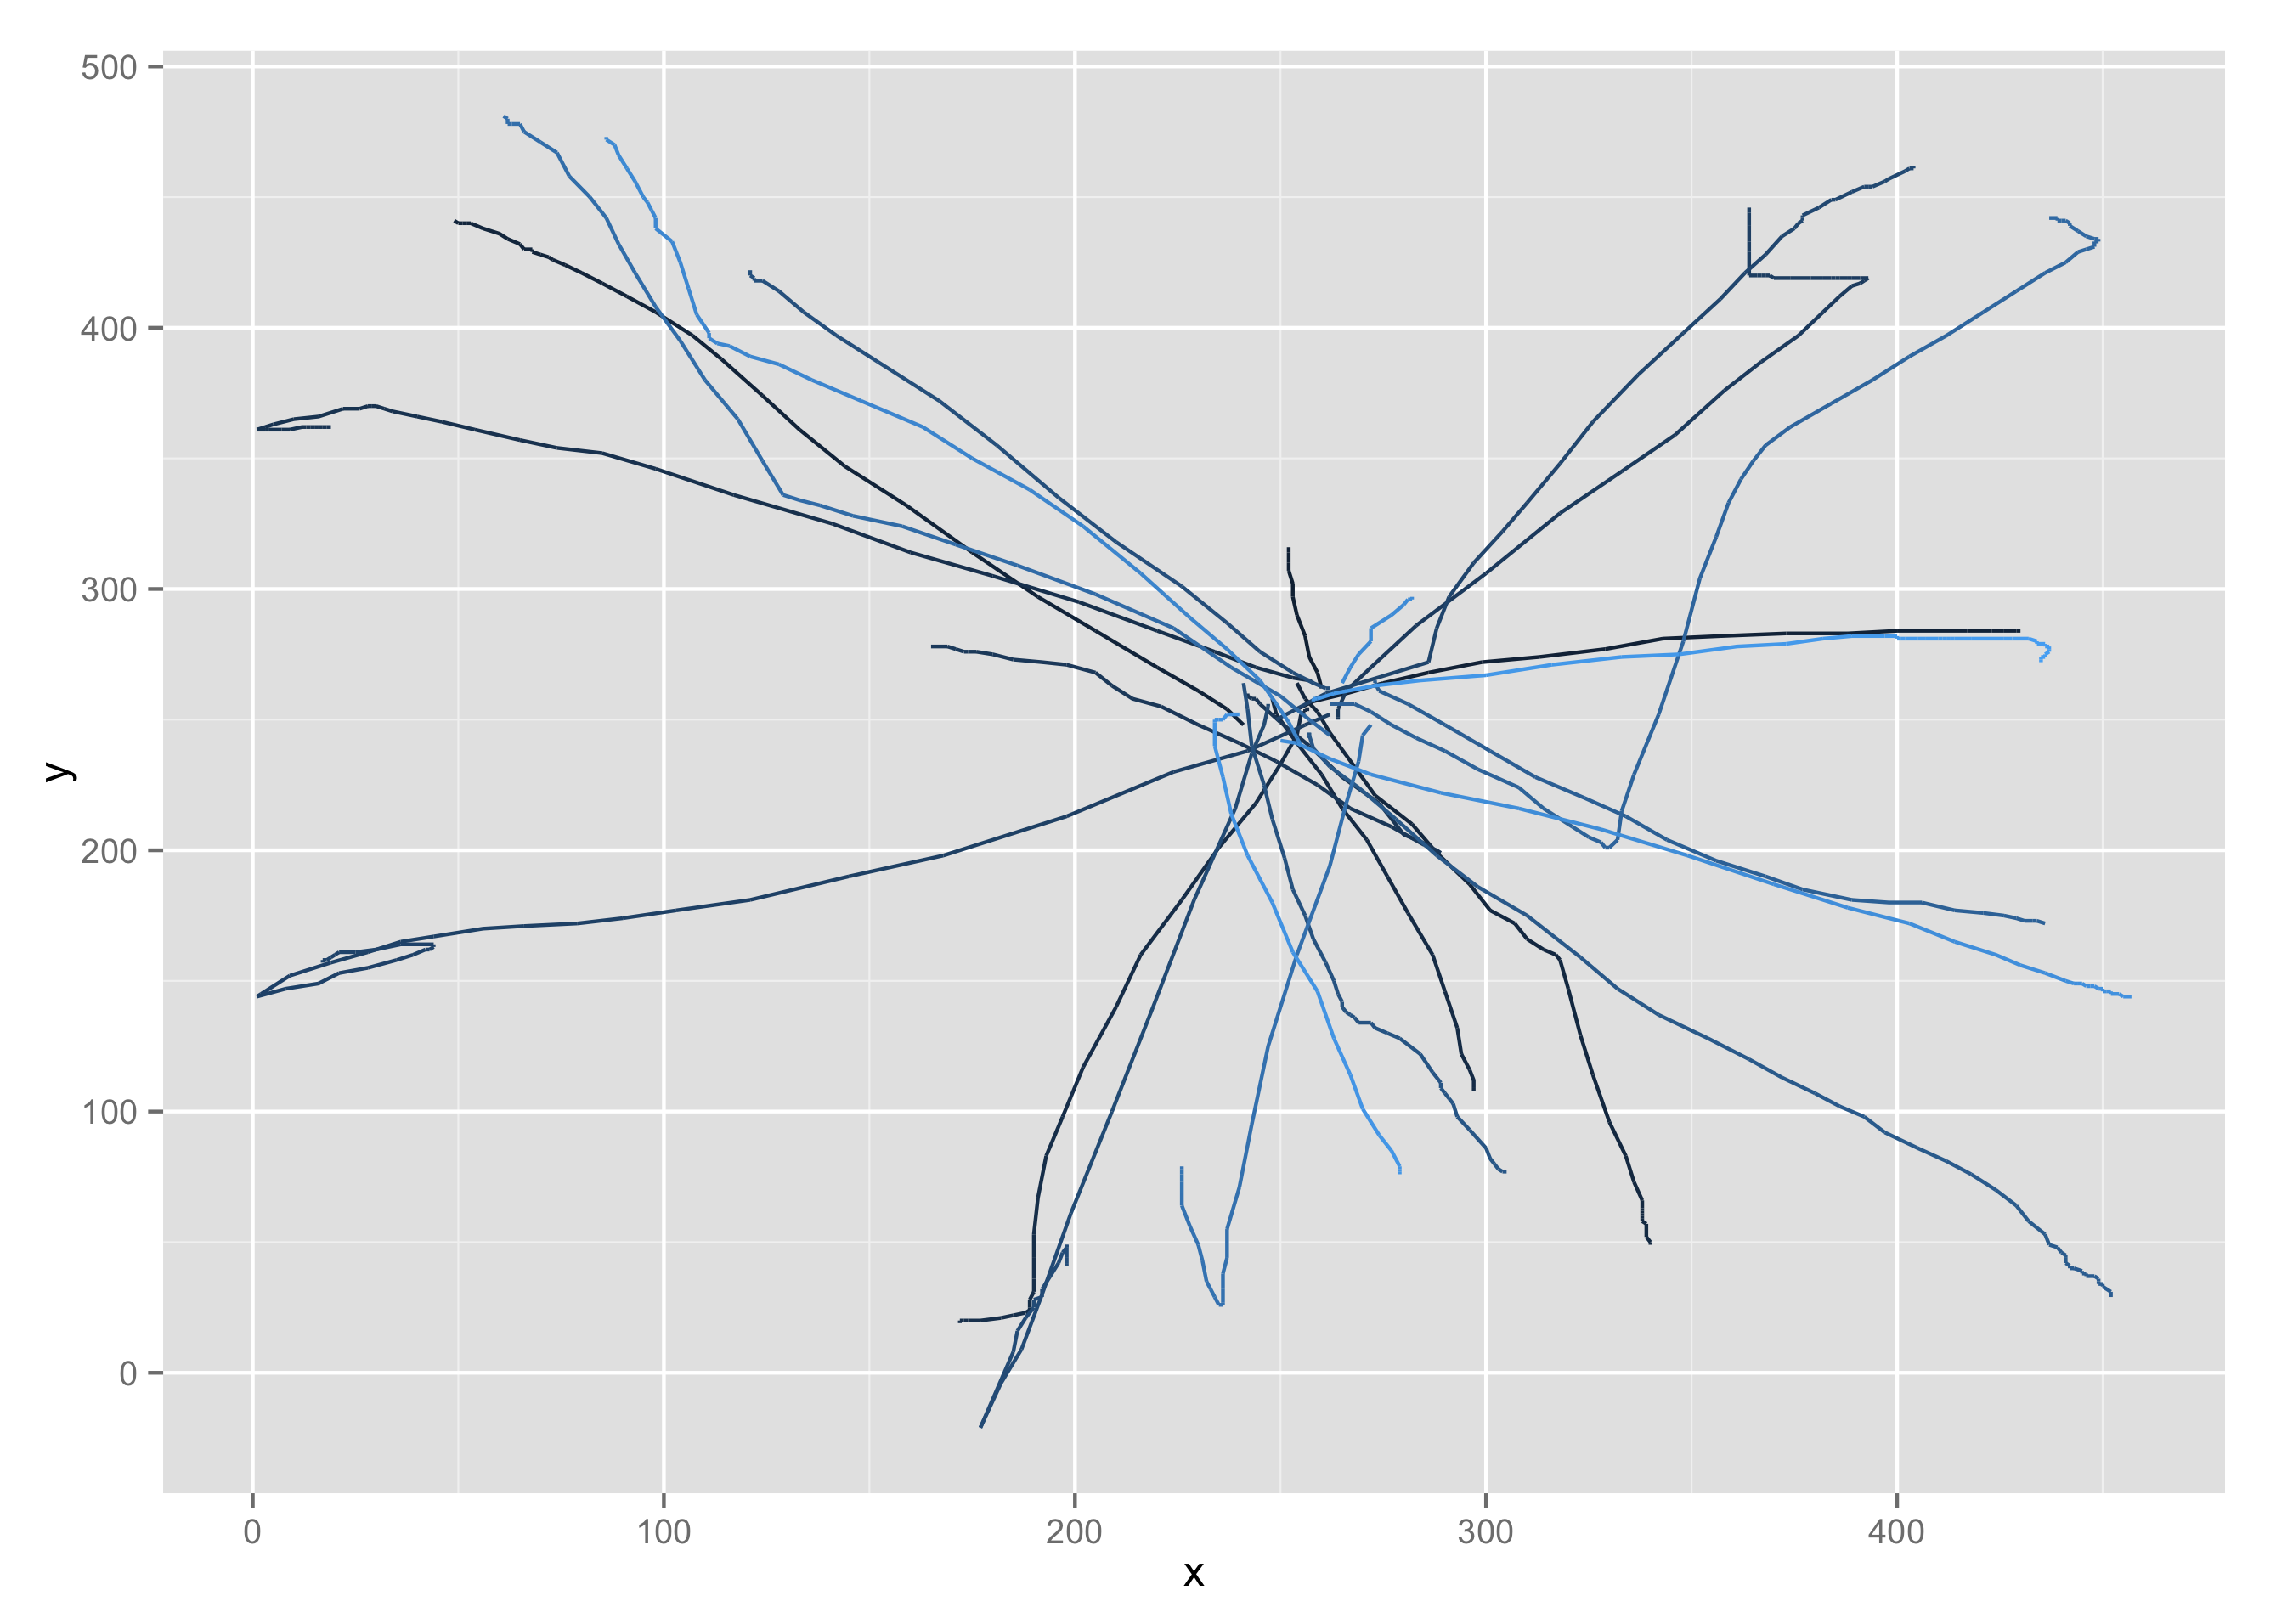
\includegraphics[width=\linewidth]{images/plots/plot_analysis_qualitative_176}
	\end{minipage}
	\begin{minipage}{0.5\linewidth}
		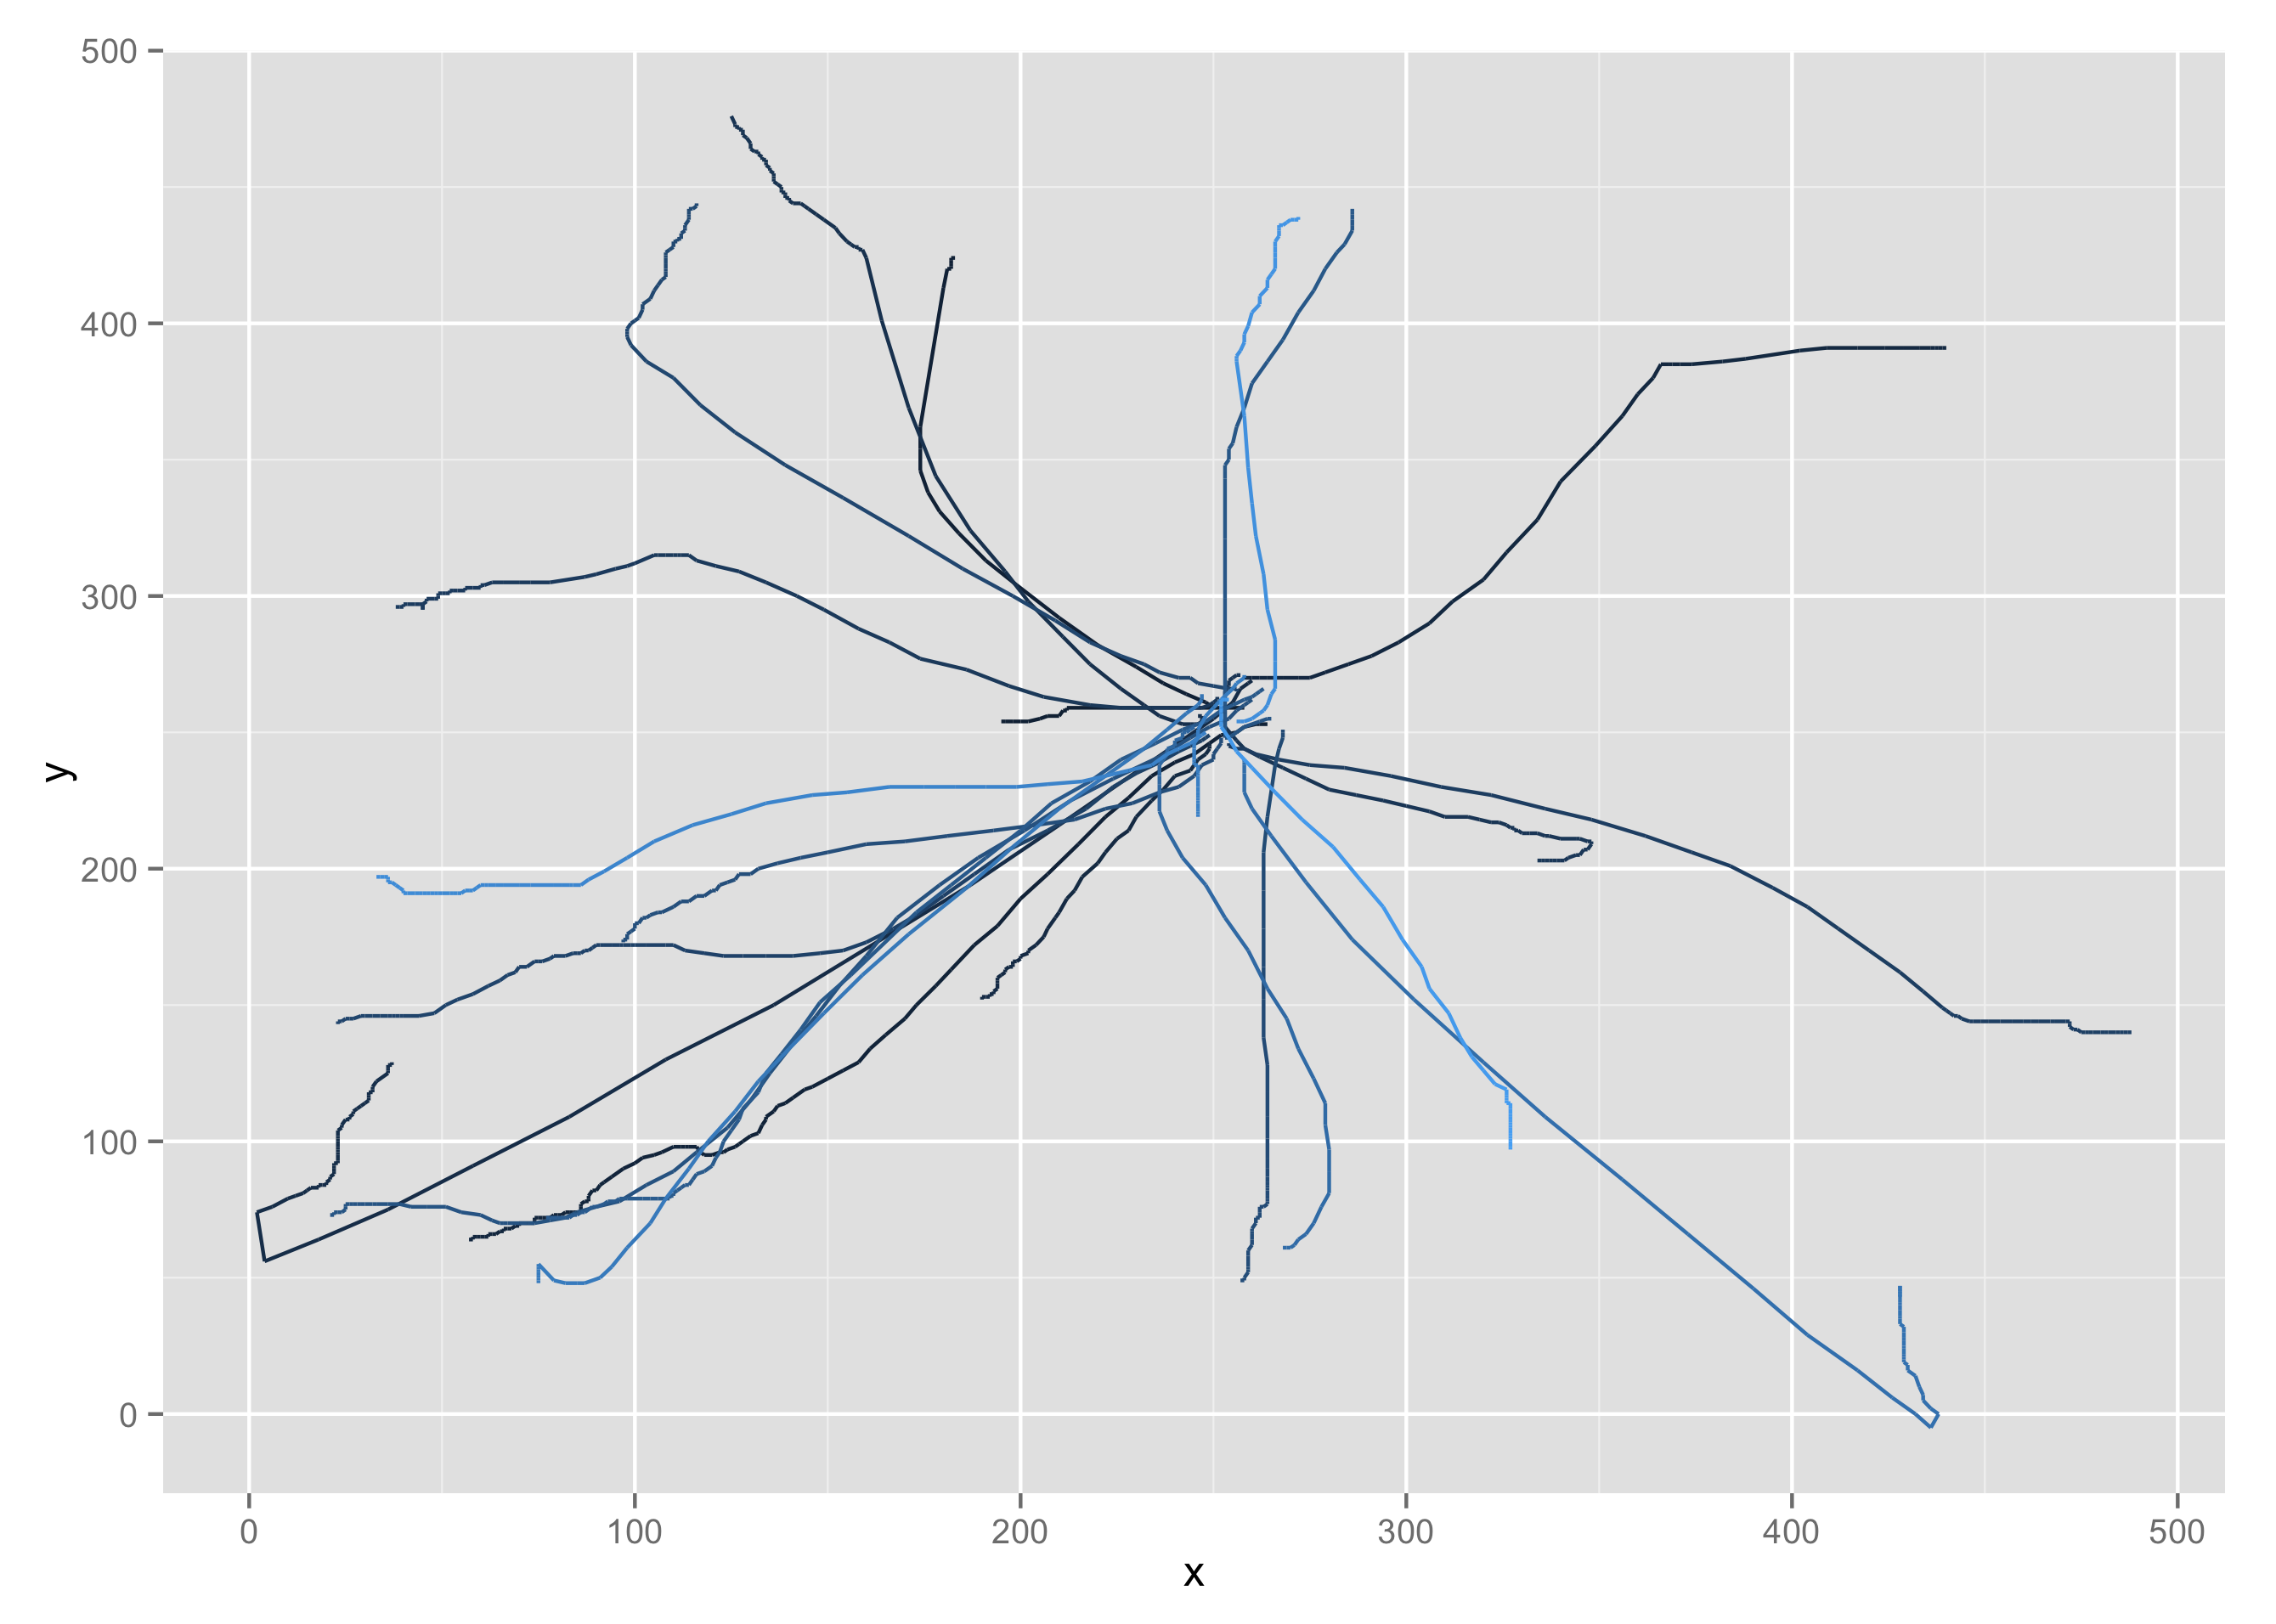
\includegraphics[width=\linewidth]{images/plots/plot_analysis_qualitative_154}
	\end{minipage}
	\captionof{figure}{8 testdeltageres bevægelsesbaner for de 25 pegeopgaver}
	\label{fig:kvaliativ_persons_2}
\end{minipage}


\begin{minipage}{\textwidth}
	\begin{minipage}{0.5\linewidth}
		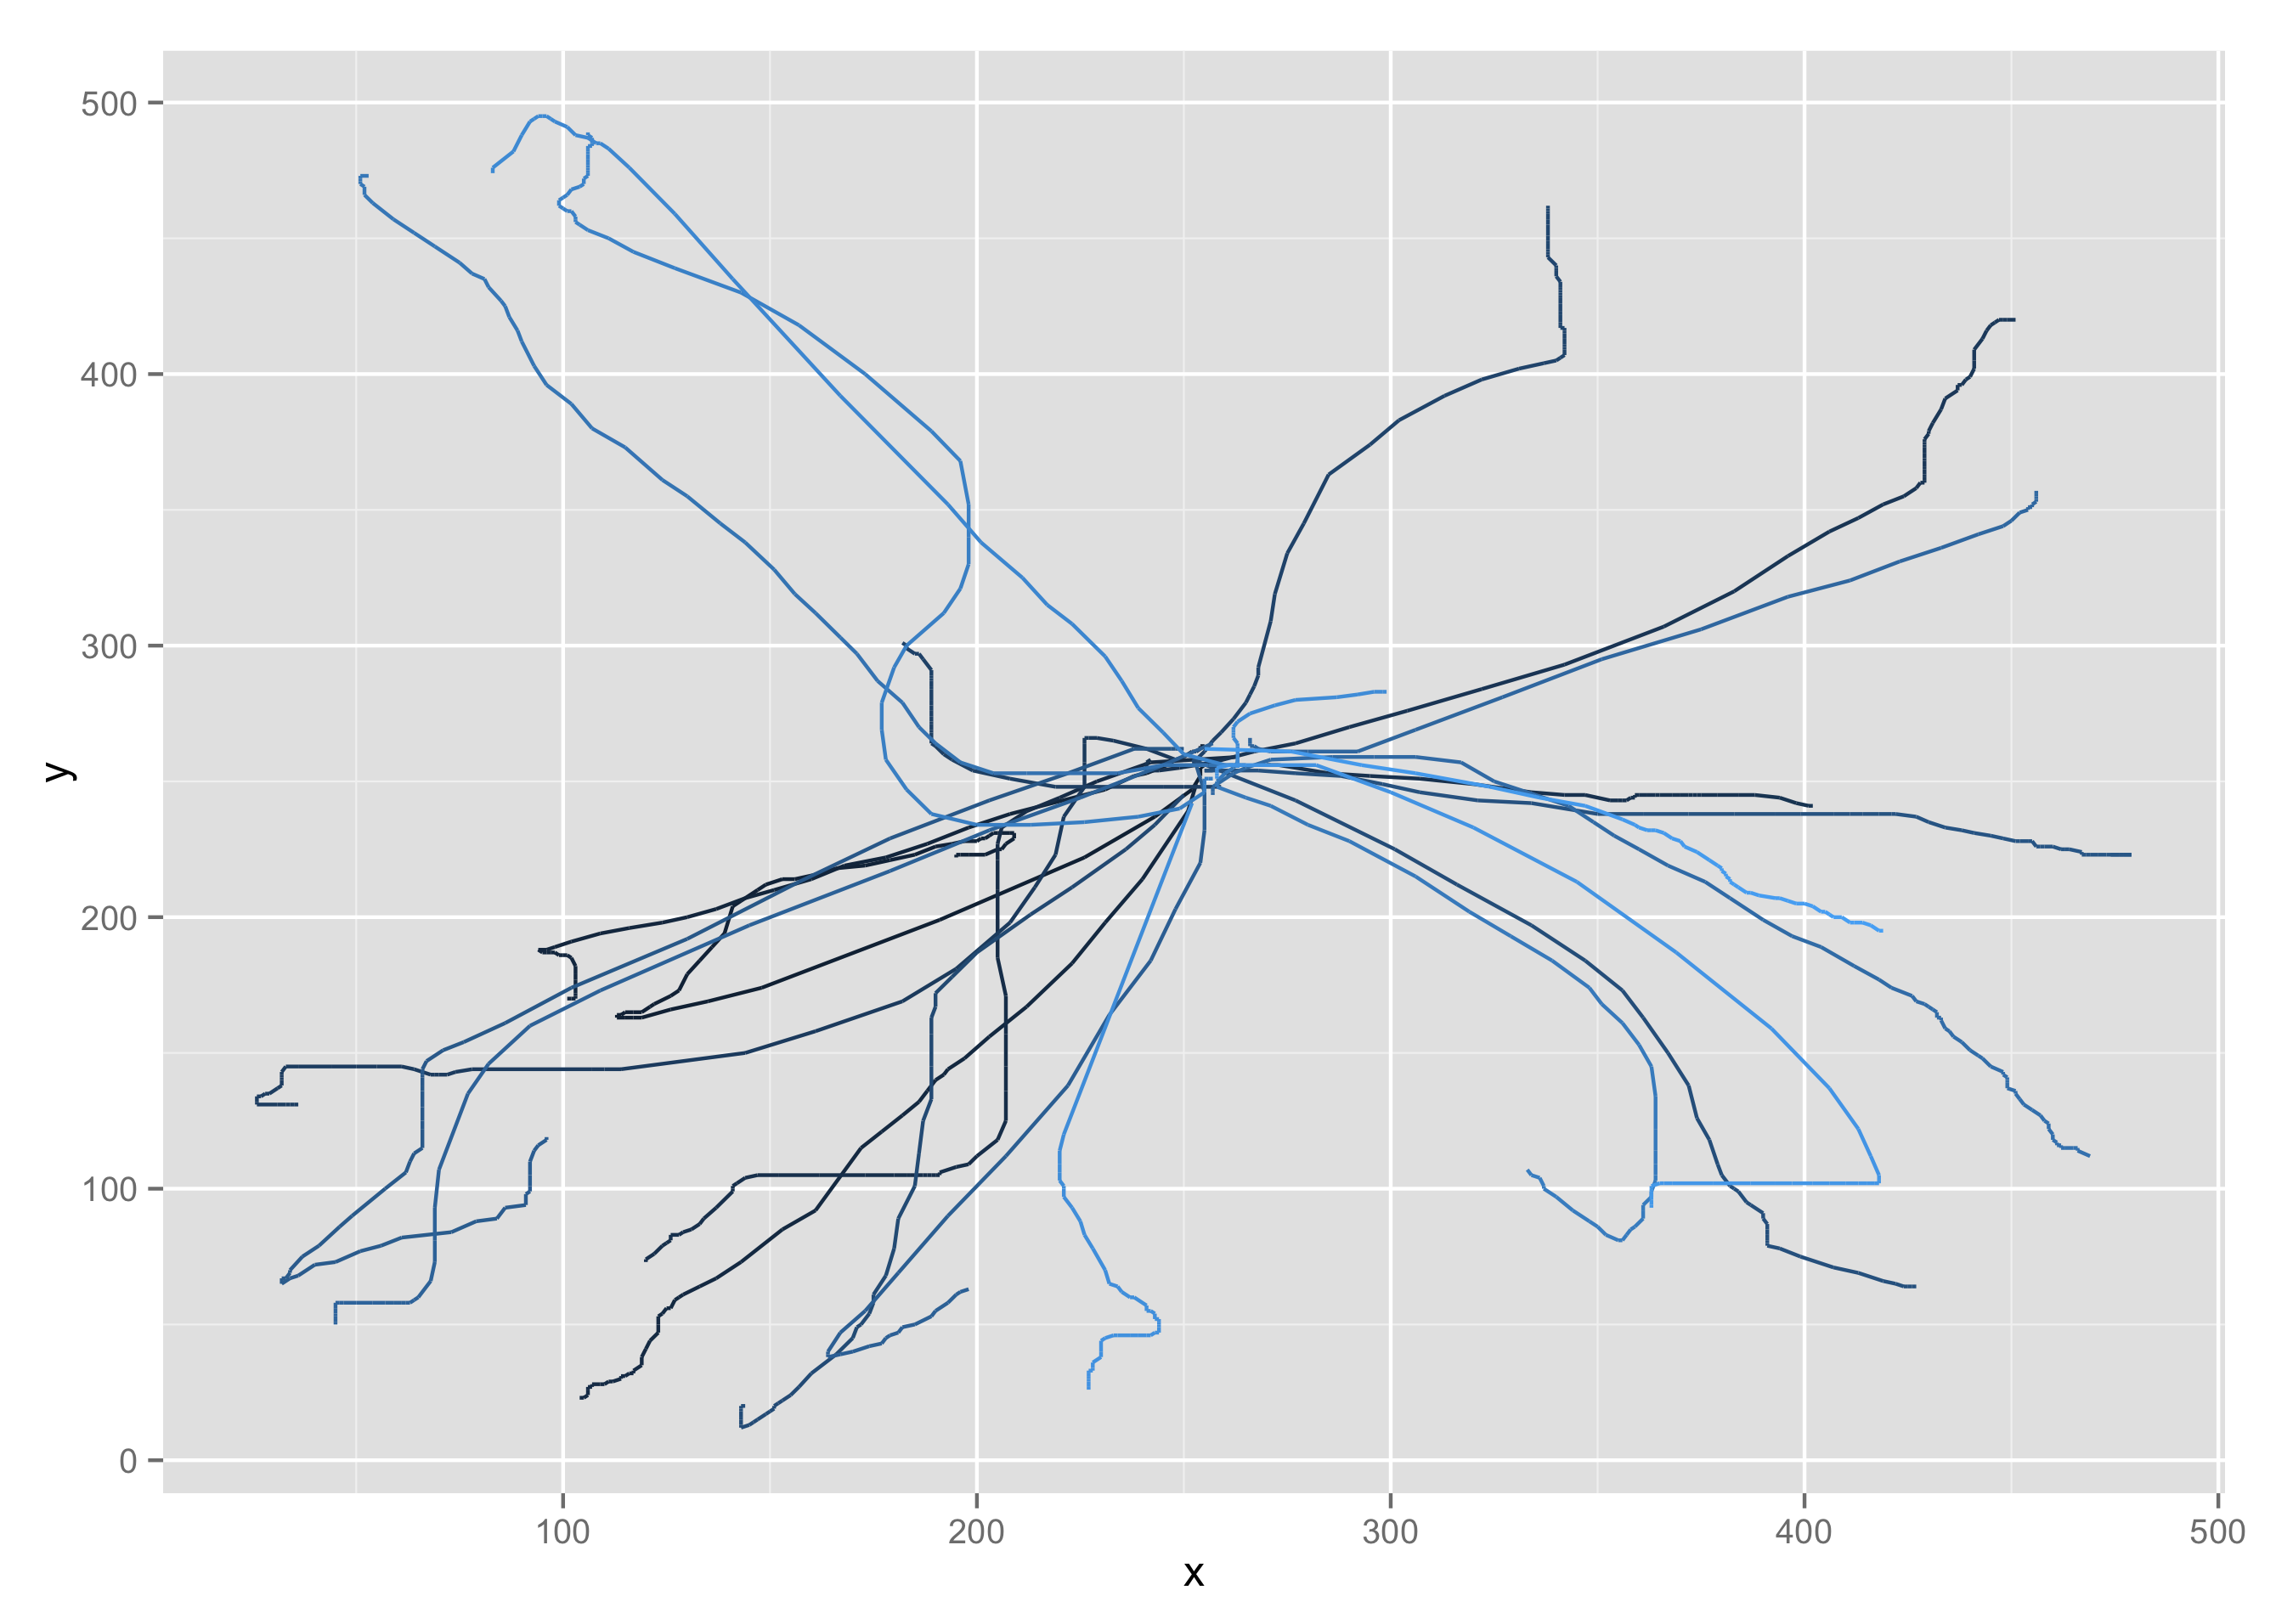
\includegraphics[width=\linewidth]{images/plots/plot_analysis_qualitative_257}
	\end{minipage}
		\begin{minipage}{0.5\linewidth}
		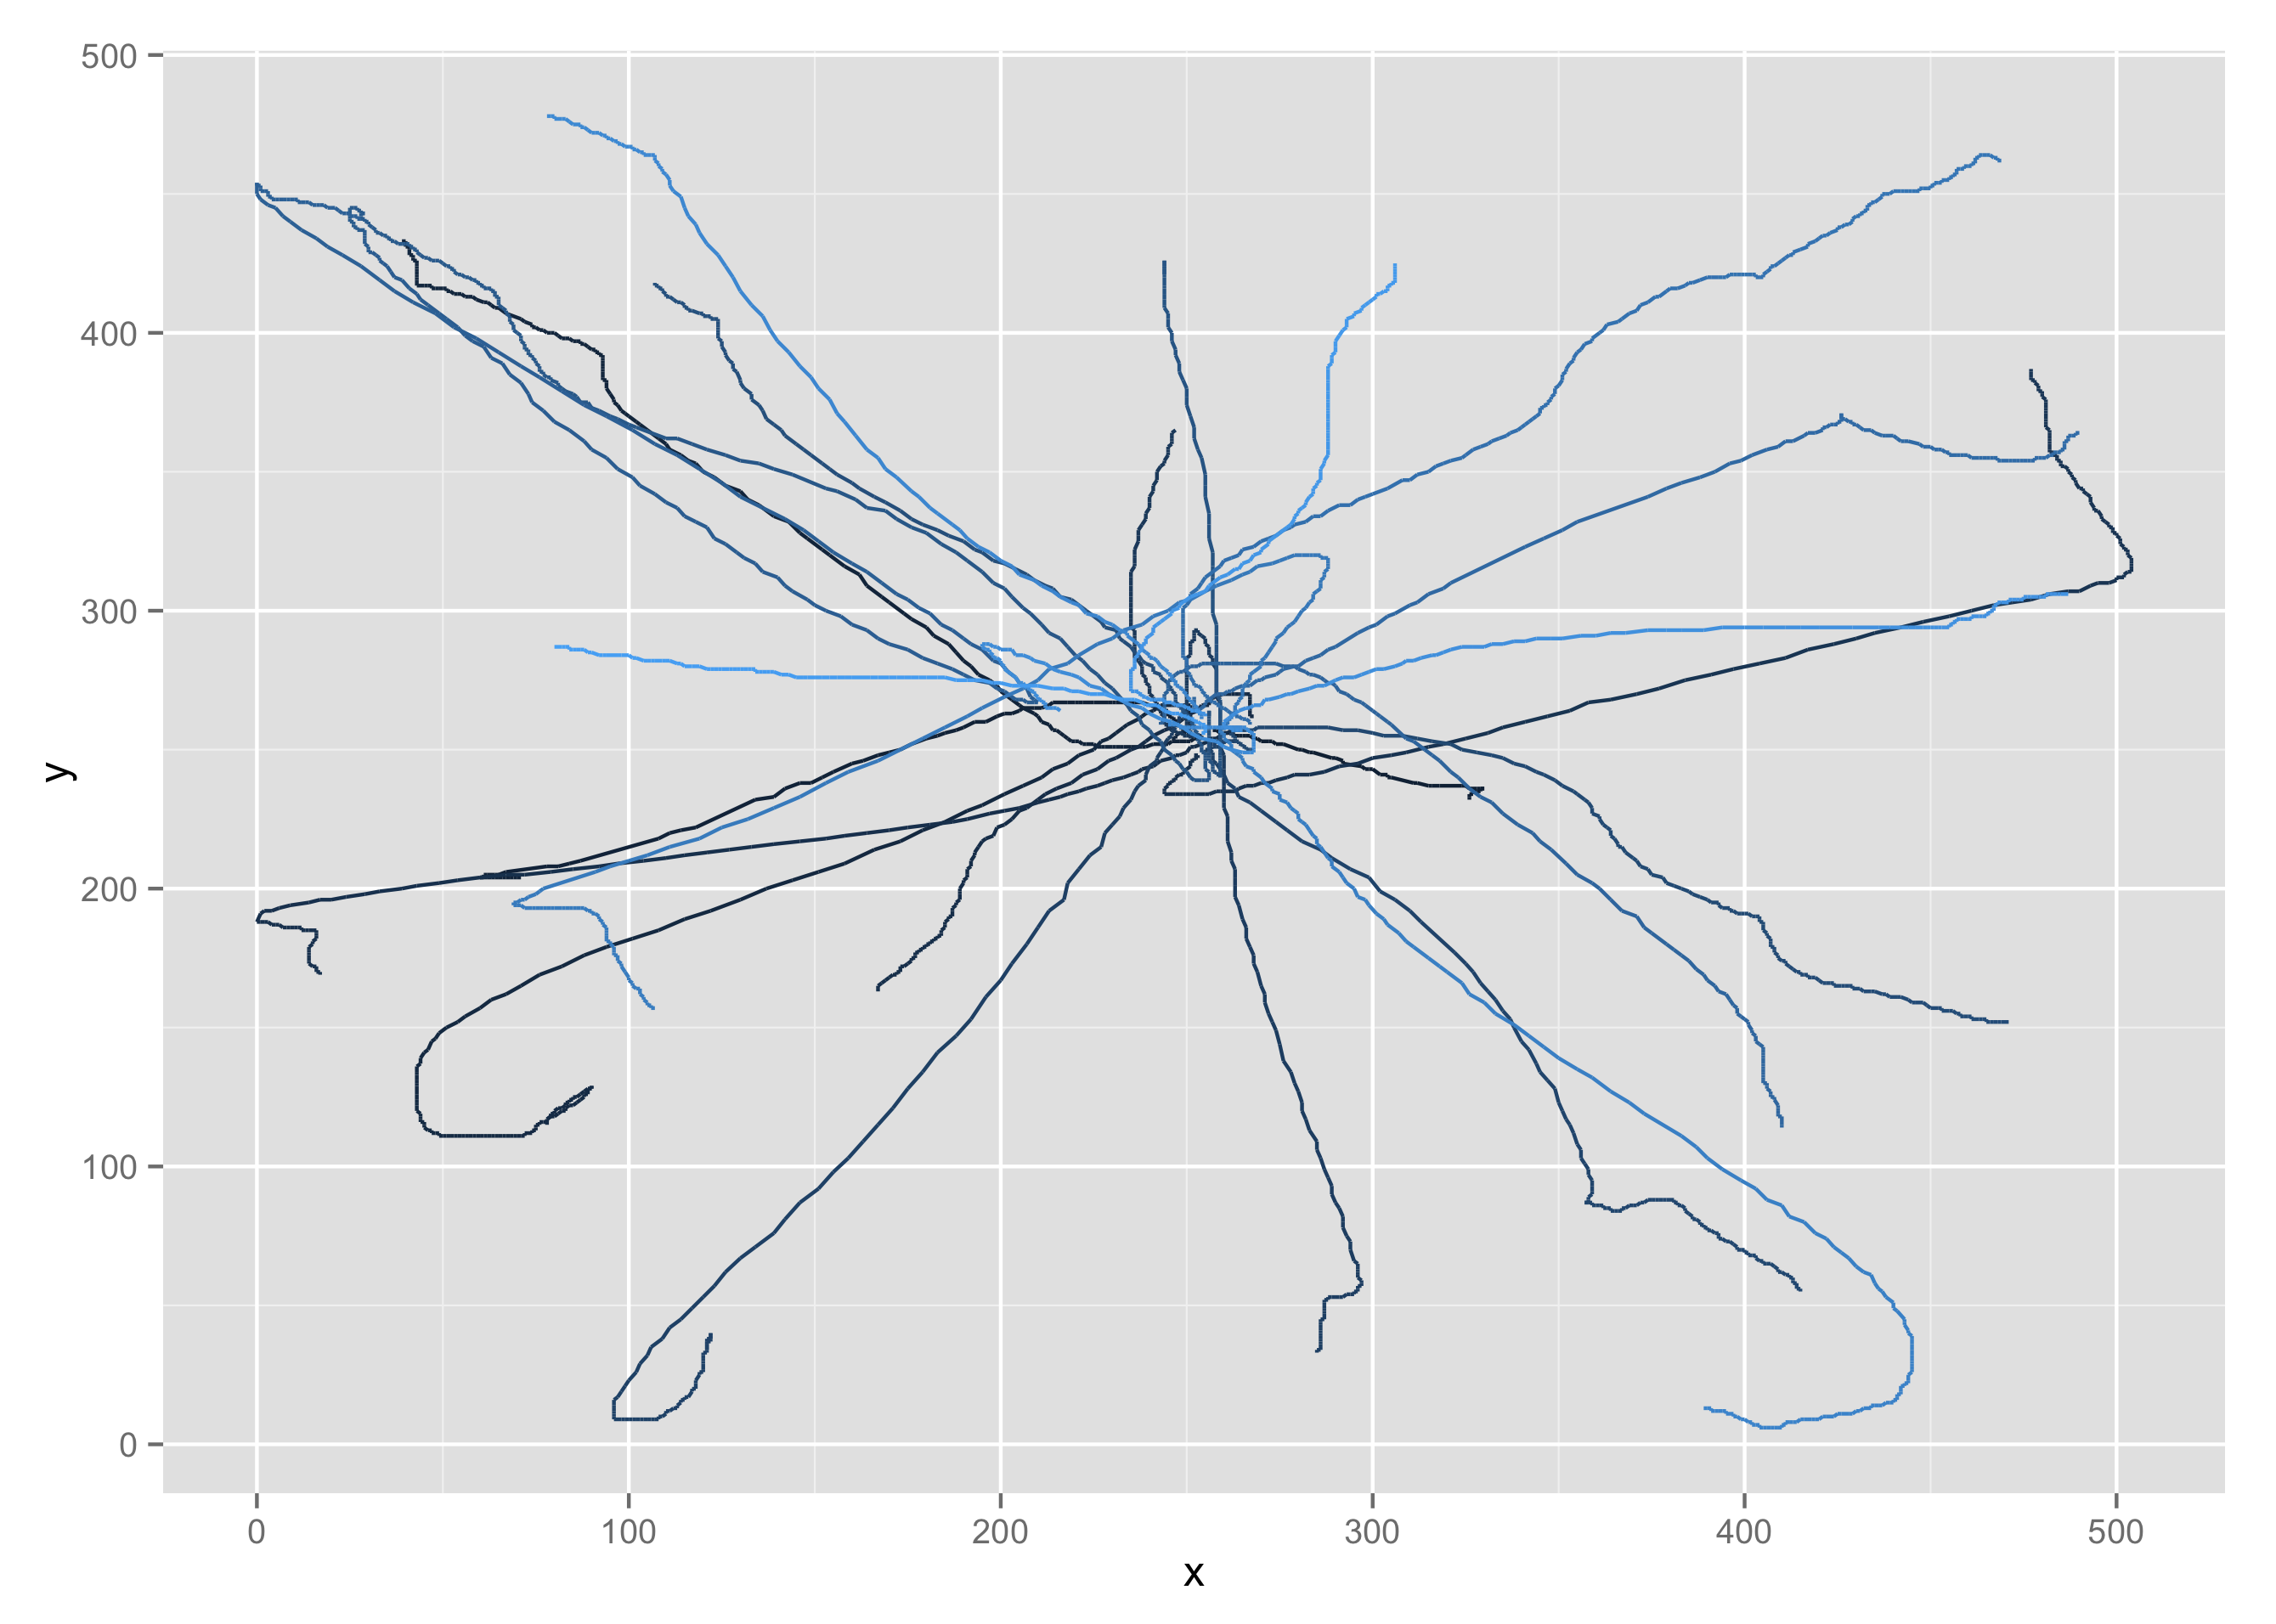
\includegraphics[width=\linewidth]{images/plots/plot_analysis_qualitative_114}
	\end{minipage}
	\begin{minipage}{0.5\linewidth}
		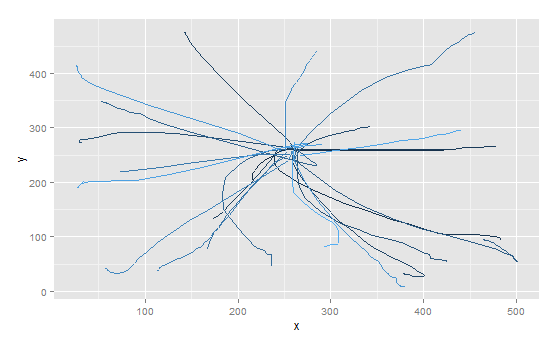
\includegraphics[width=\linewidth]{images/plots/plot_analysis_qualitative_3}
	\end{minipage}
	\begin{minipage}{0.5\linewidth}
		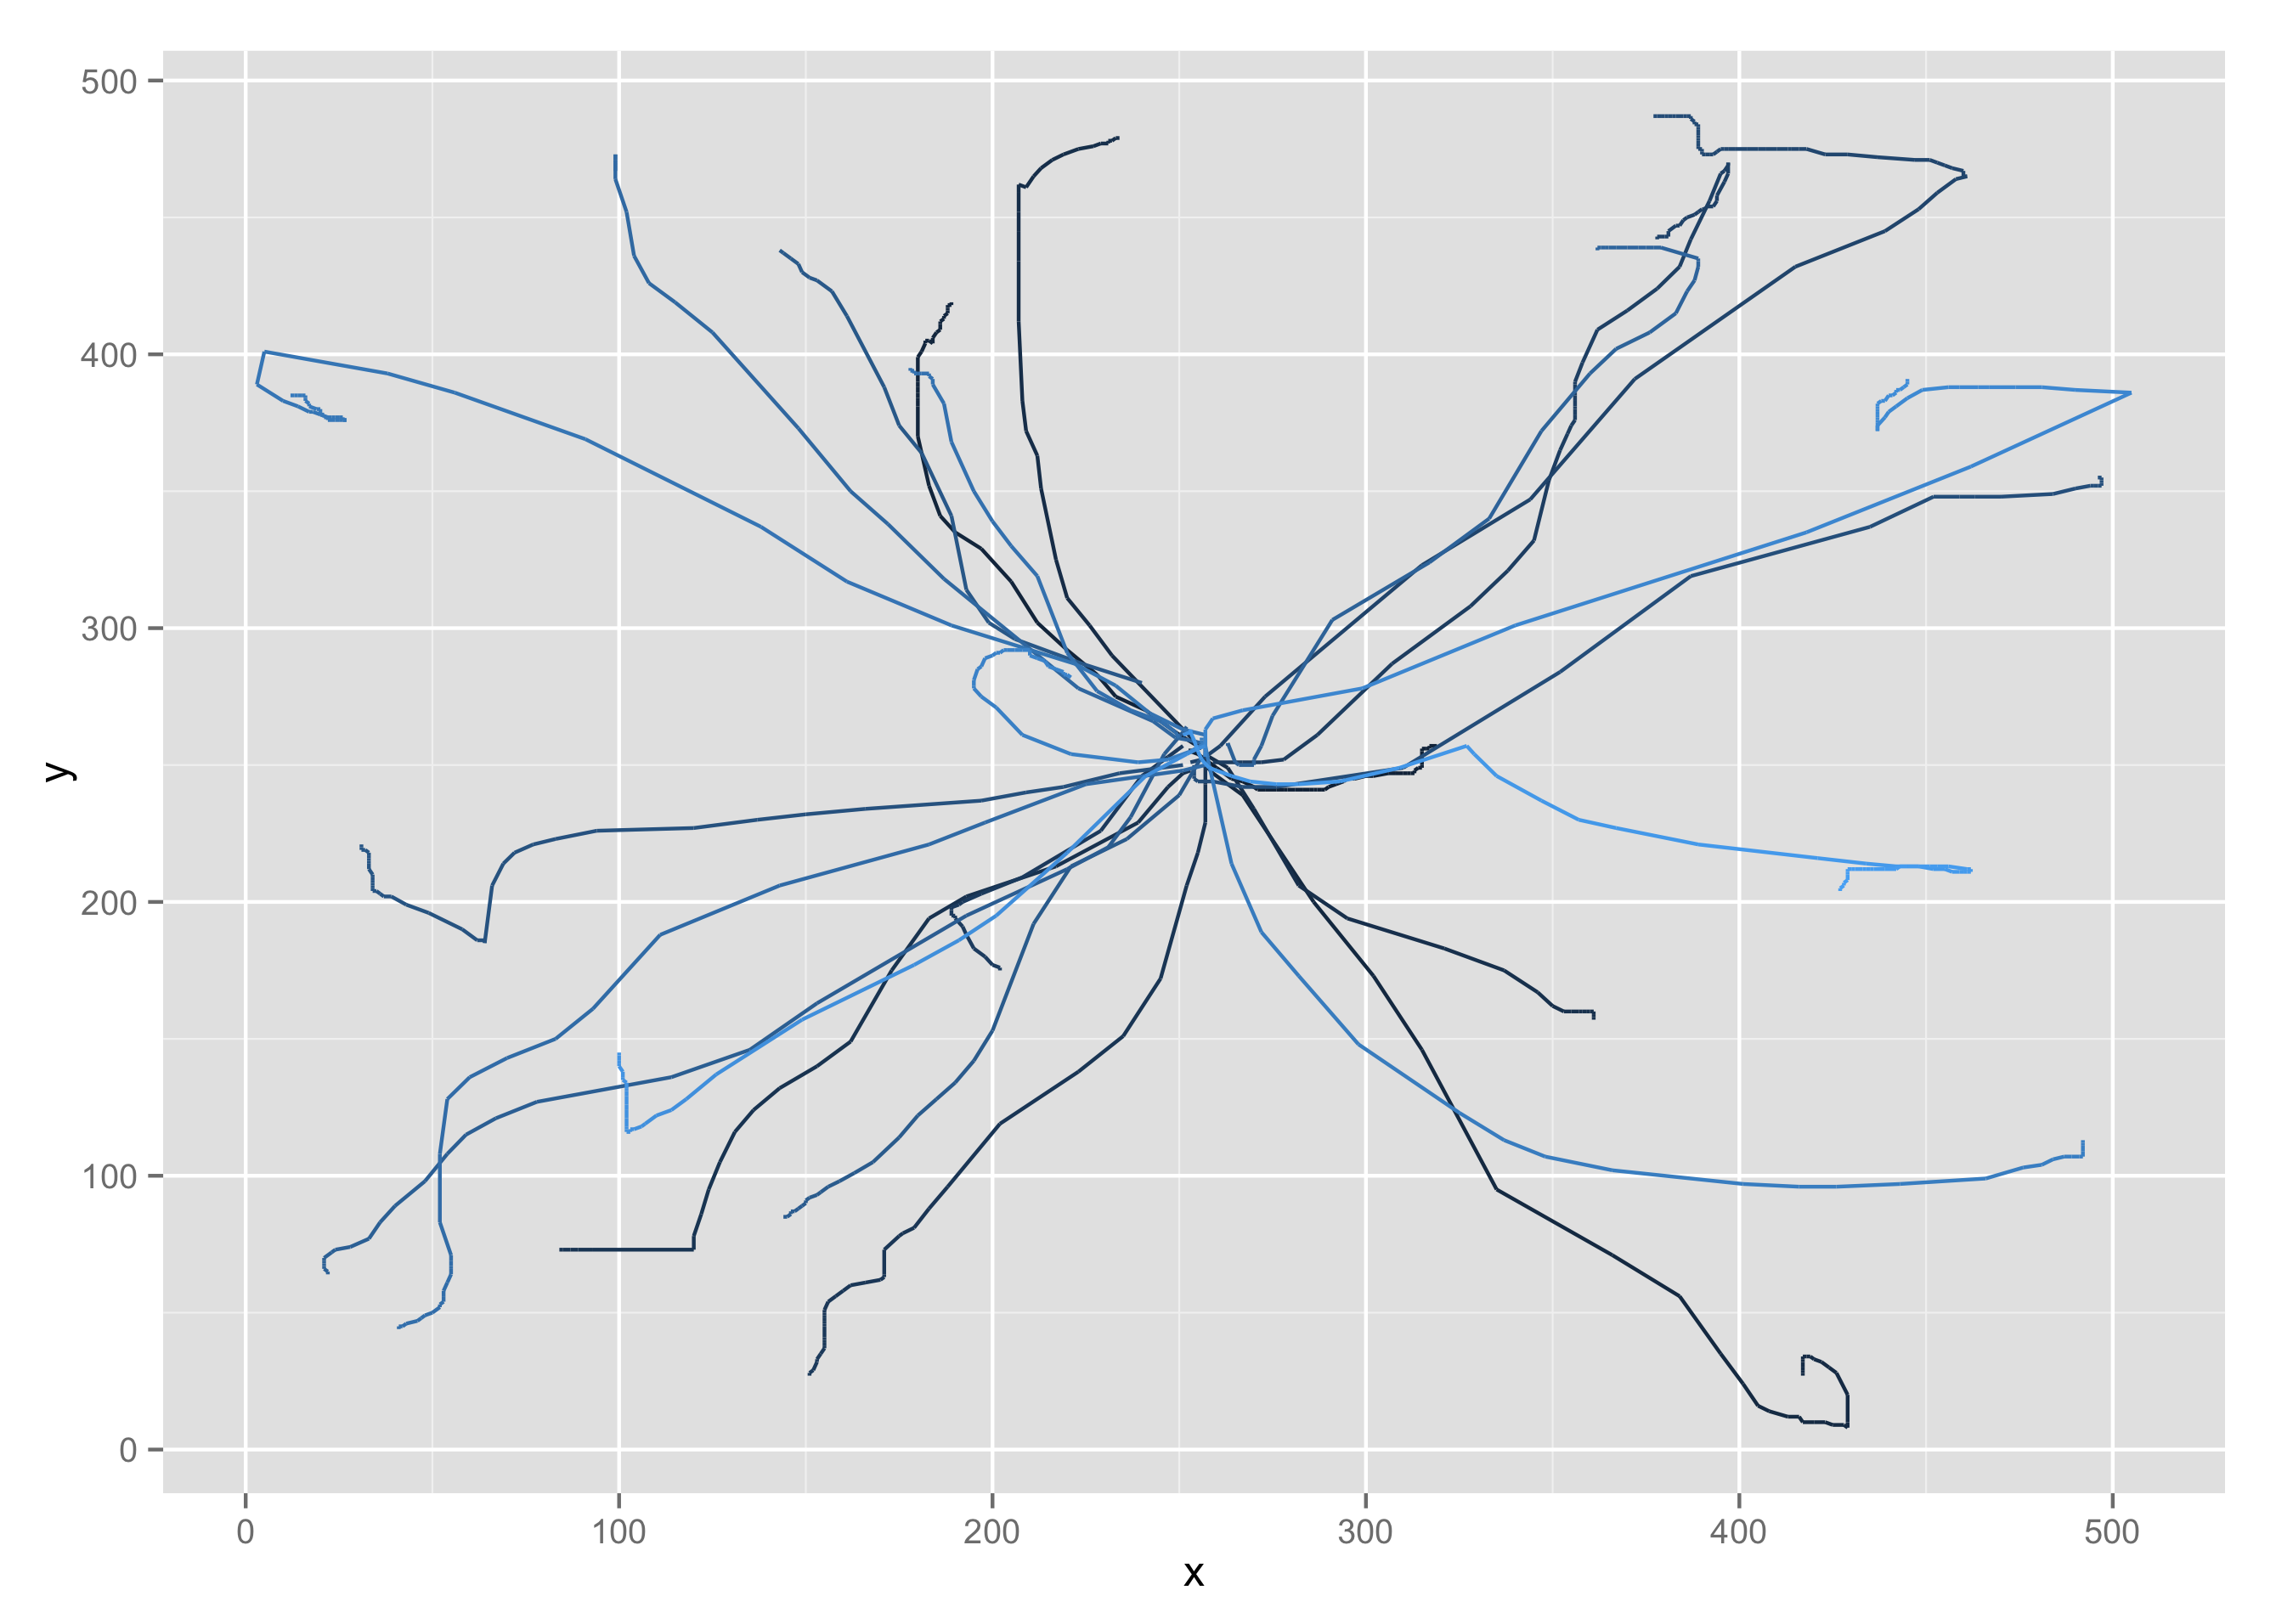
\includegraphics[width=\linewidth]{images/plots/plot_analysis_qualitative_78}
	\end{minipage}
	\begin{minipage}{0.5\linewidth}
		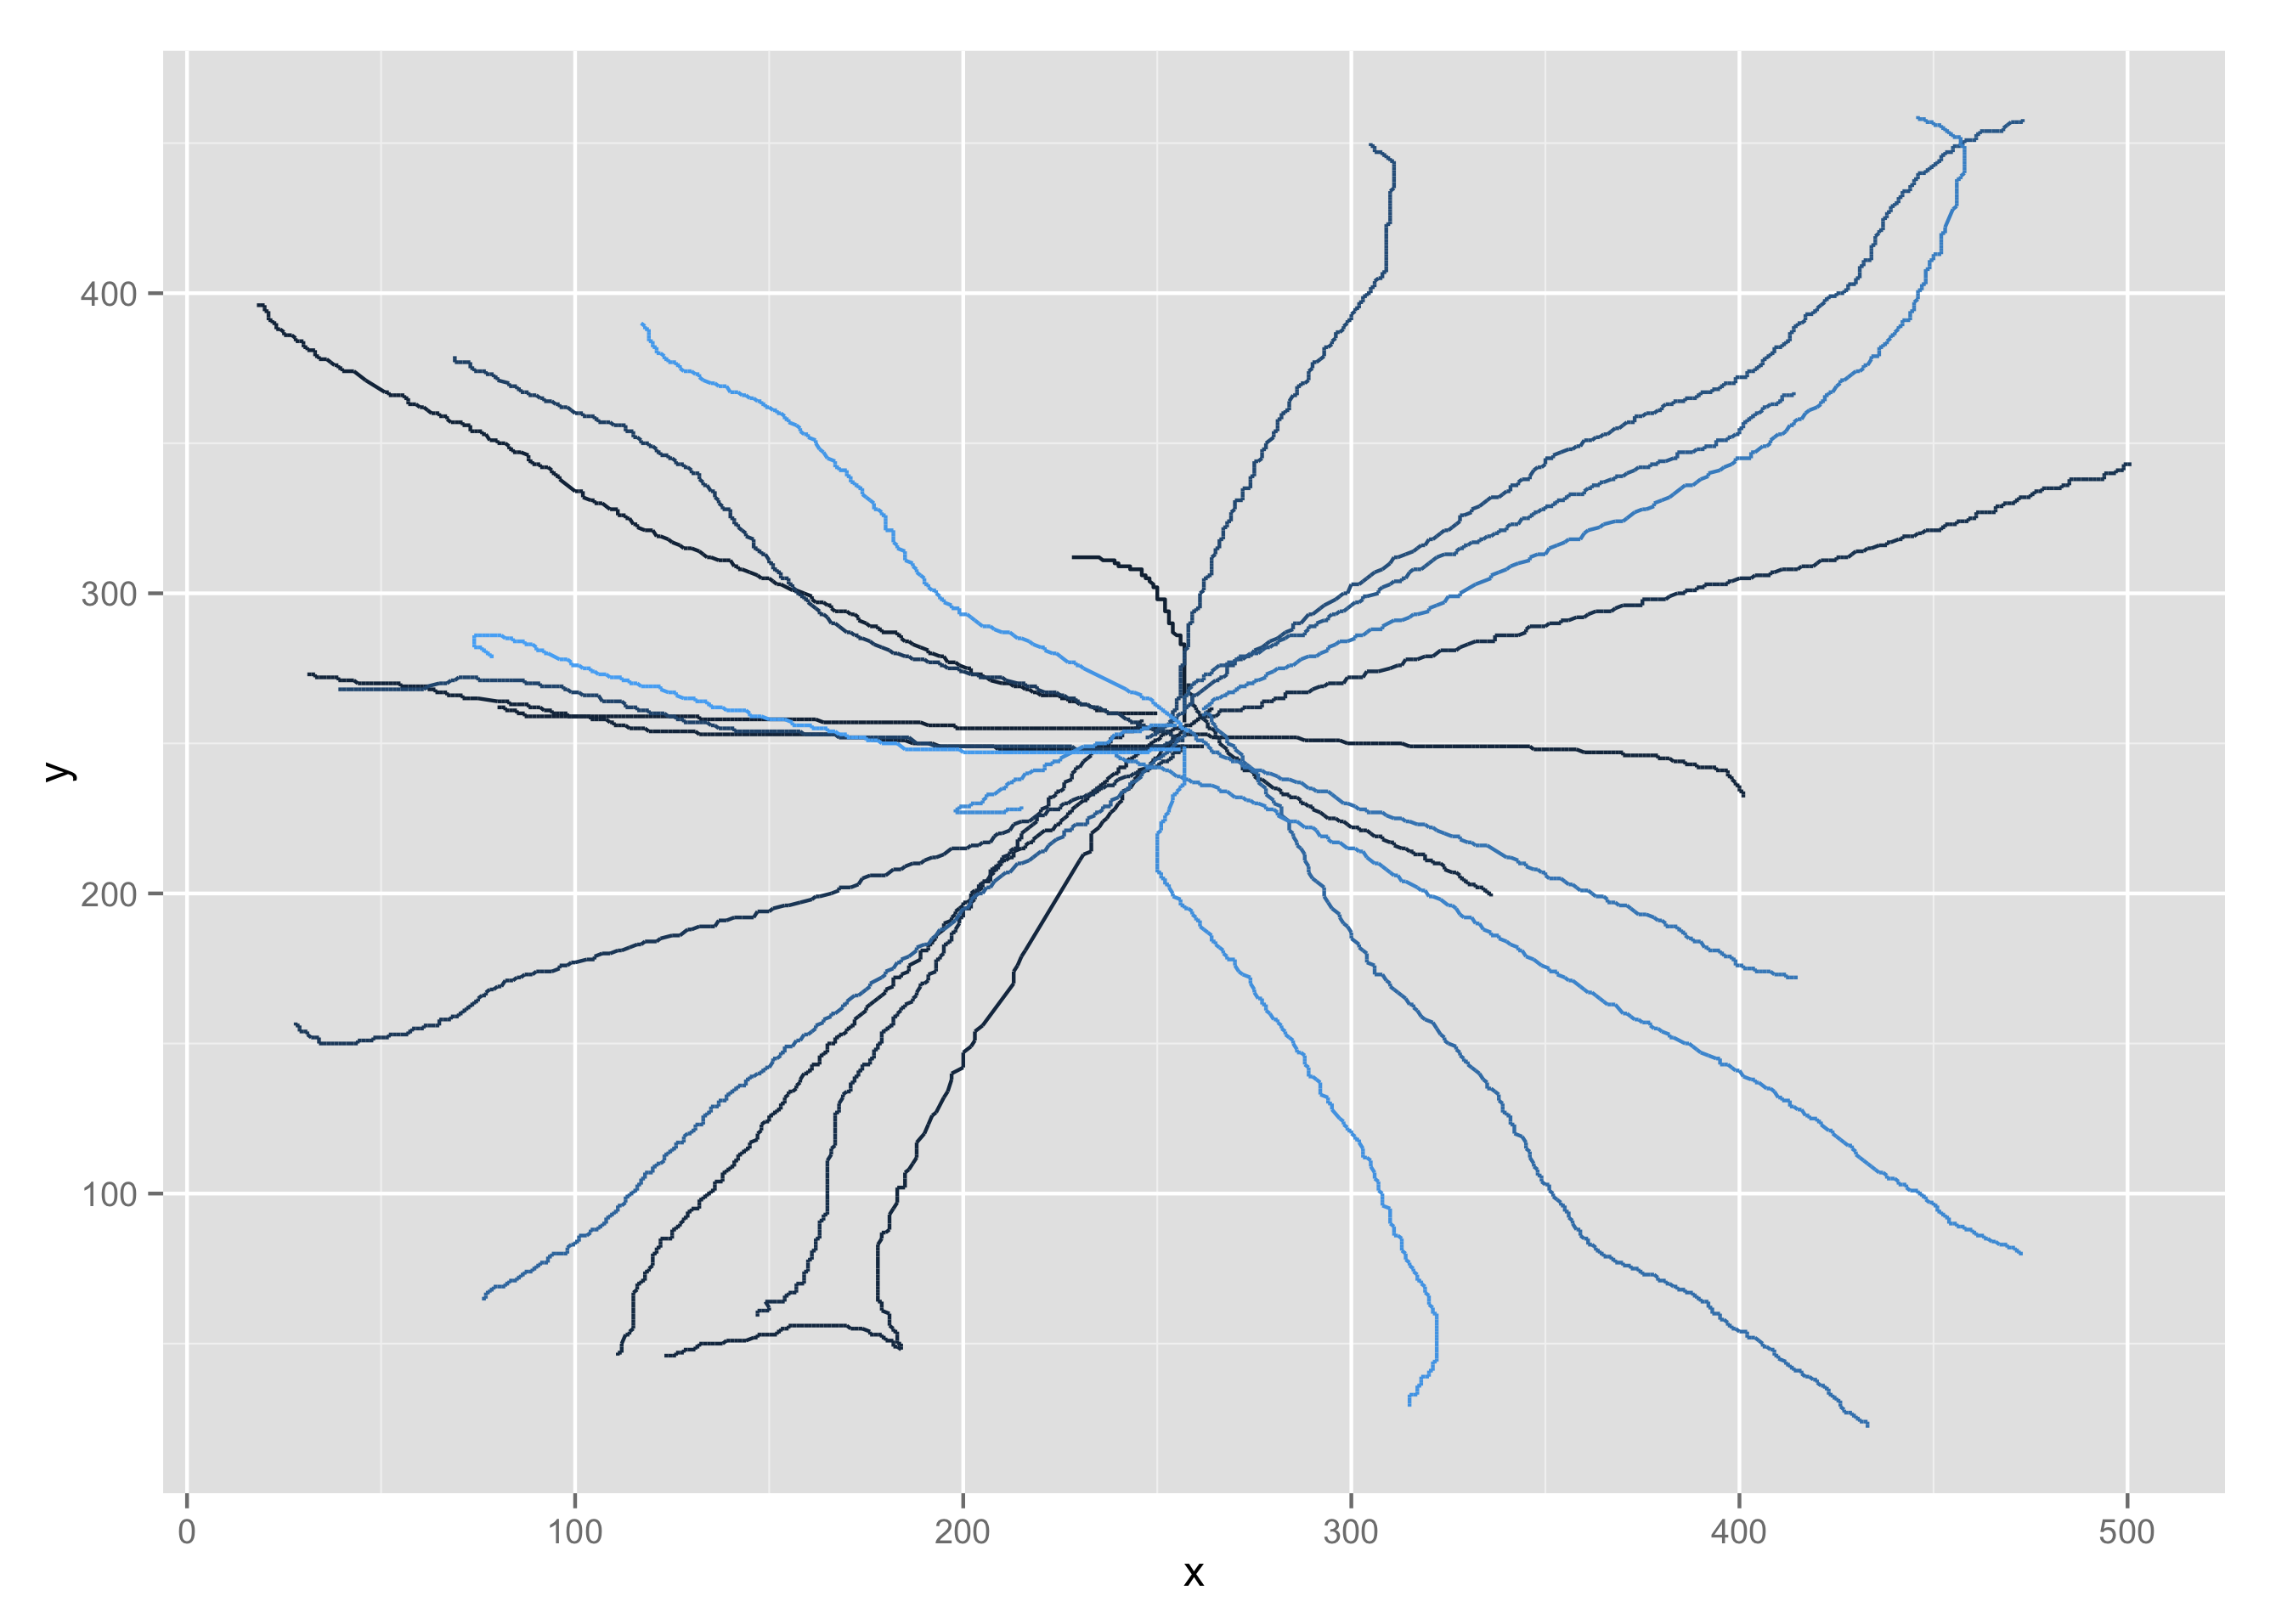
\includegraphics[width=\linewidth]{images/plots/plot_analysis_qualitative_171}
	\end{minipage}
	\begin{minipage}{0.5\linewidth}
		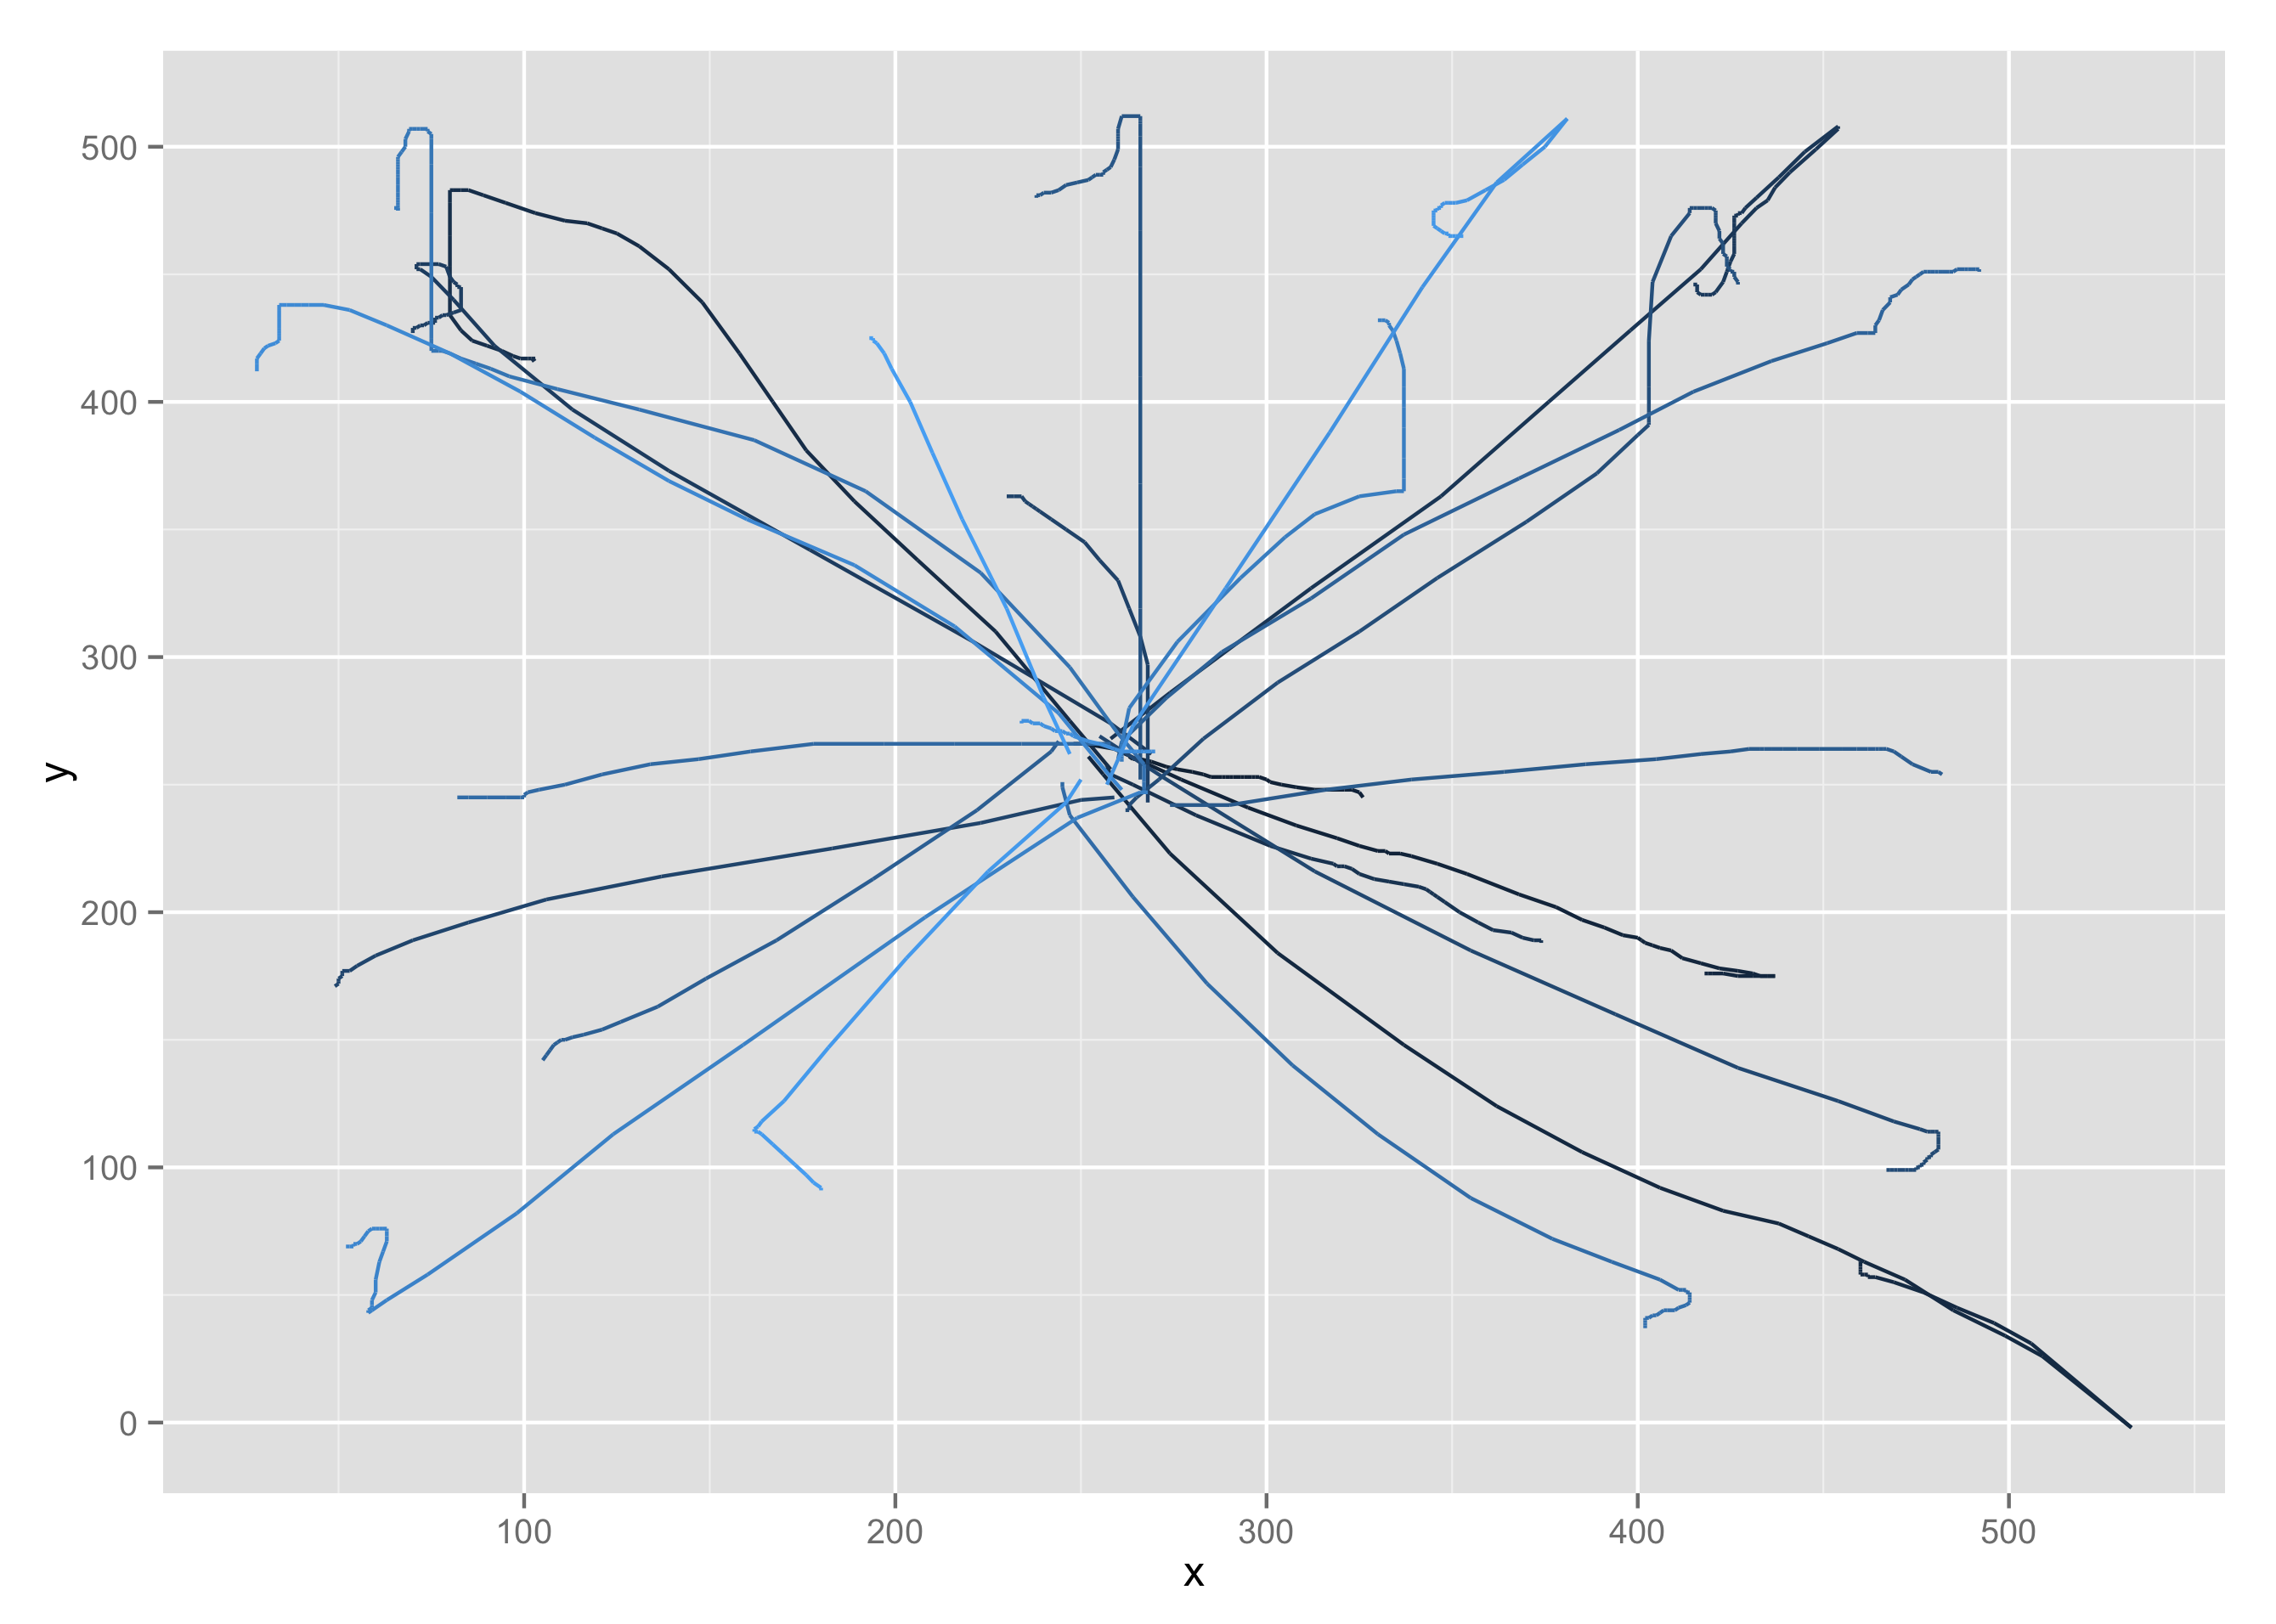
\includegraphics[width=\linewidth]{images/plots/plot_analysis_qualitative_219}
	\end{minipage}
	\captionof{figure}{6 testdeltageres bevægelsesbaner for de 25 pegeopgaver}
	\label{fig:kvaliativ_persons_3}
\end{minipage}

%-- Fartprofiler --%
\chapter{Fartprofiler for 8 testdeltagere}
\label{sec:speed_plots}
\begin{minipage}{\textwidth}
	\begin{minipage}{0.5\linewidth}
		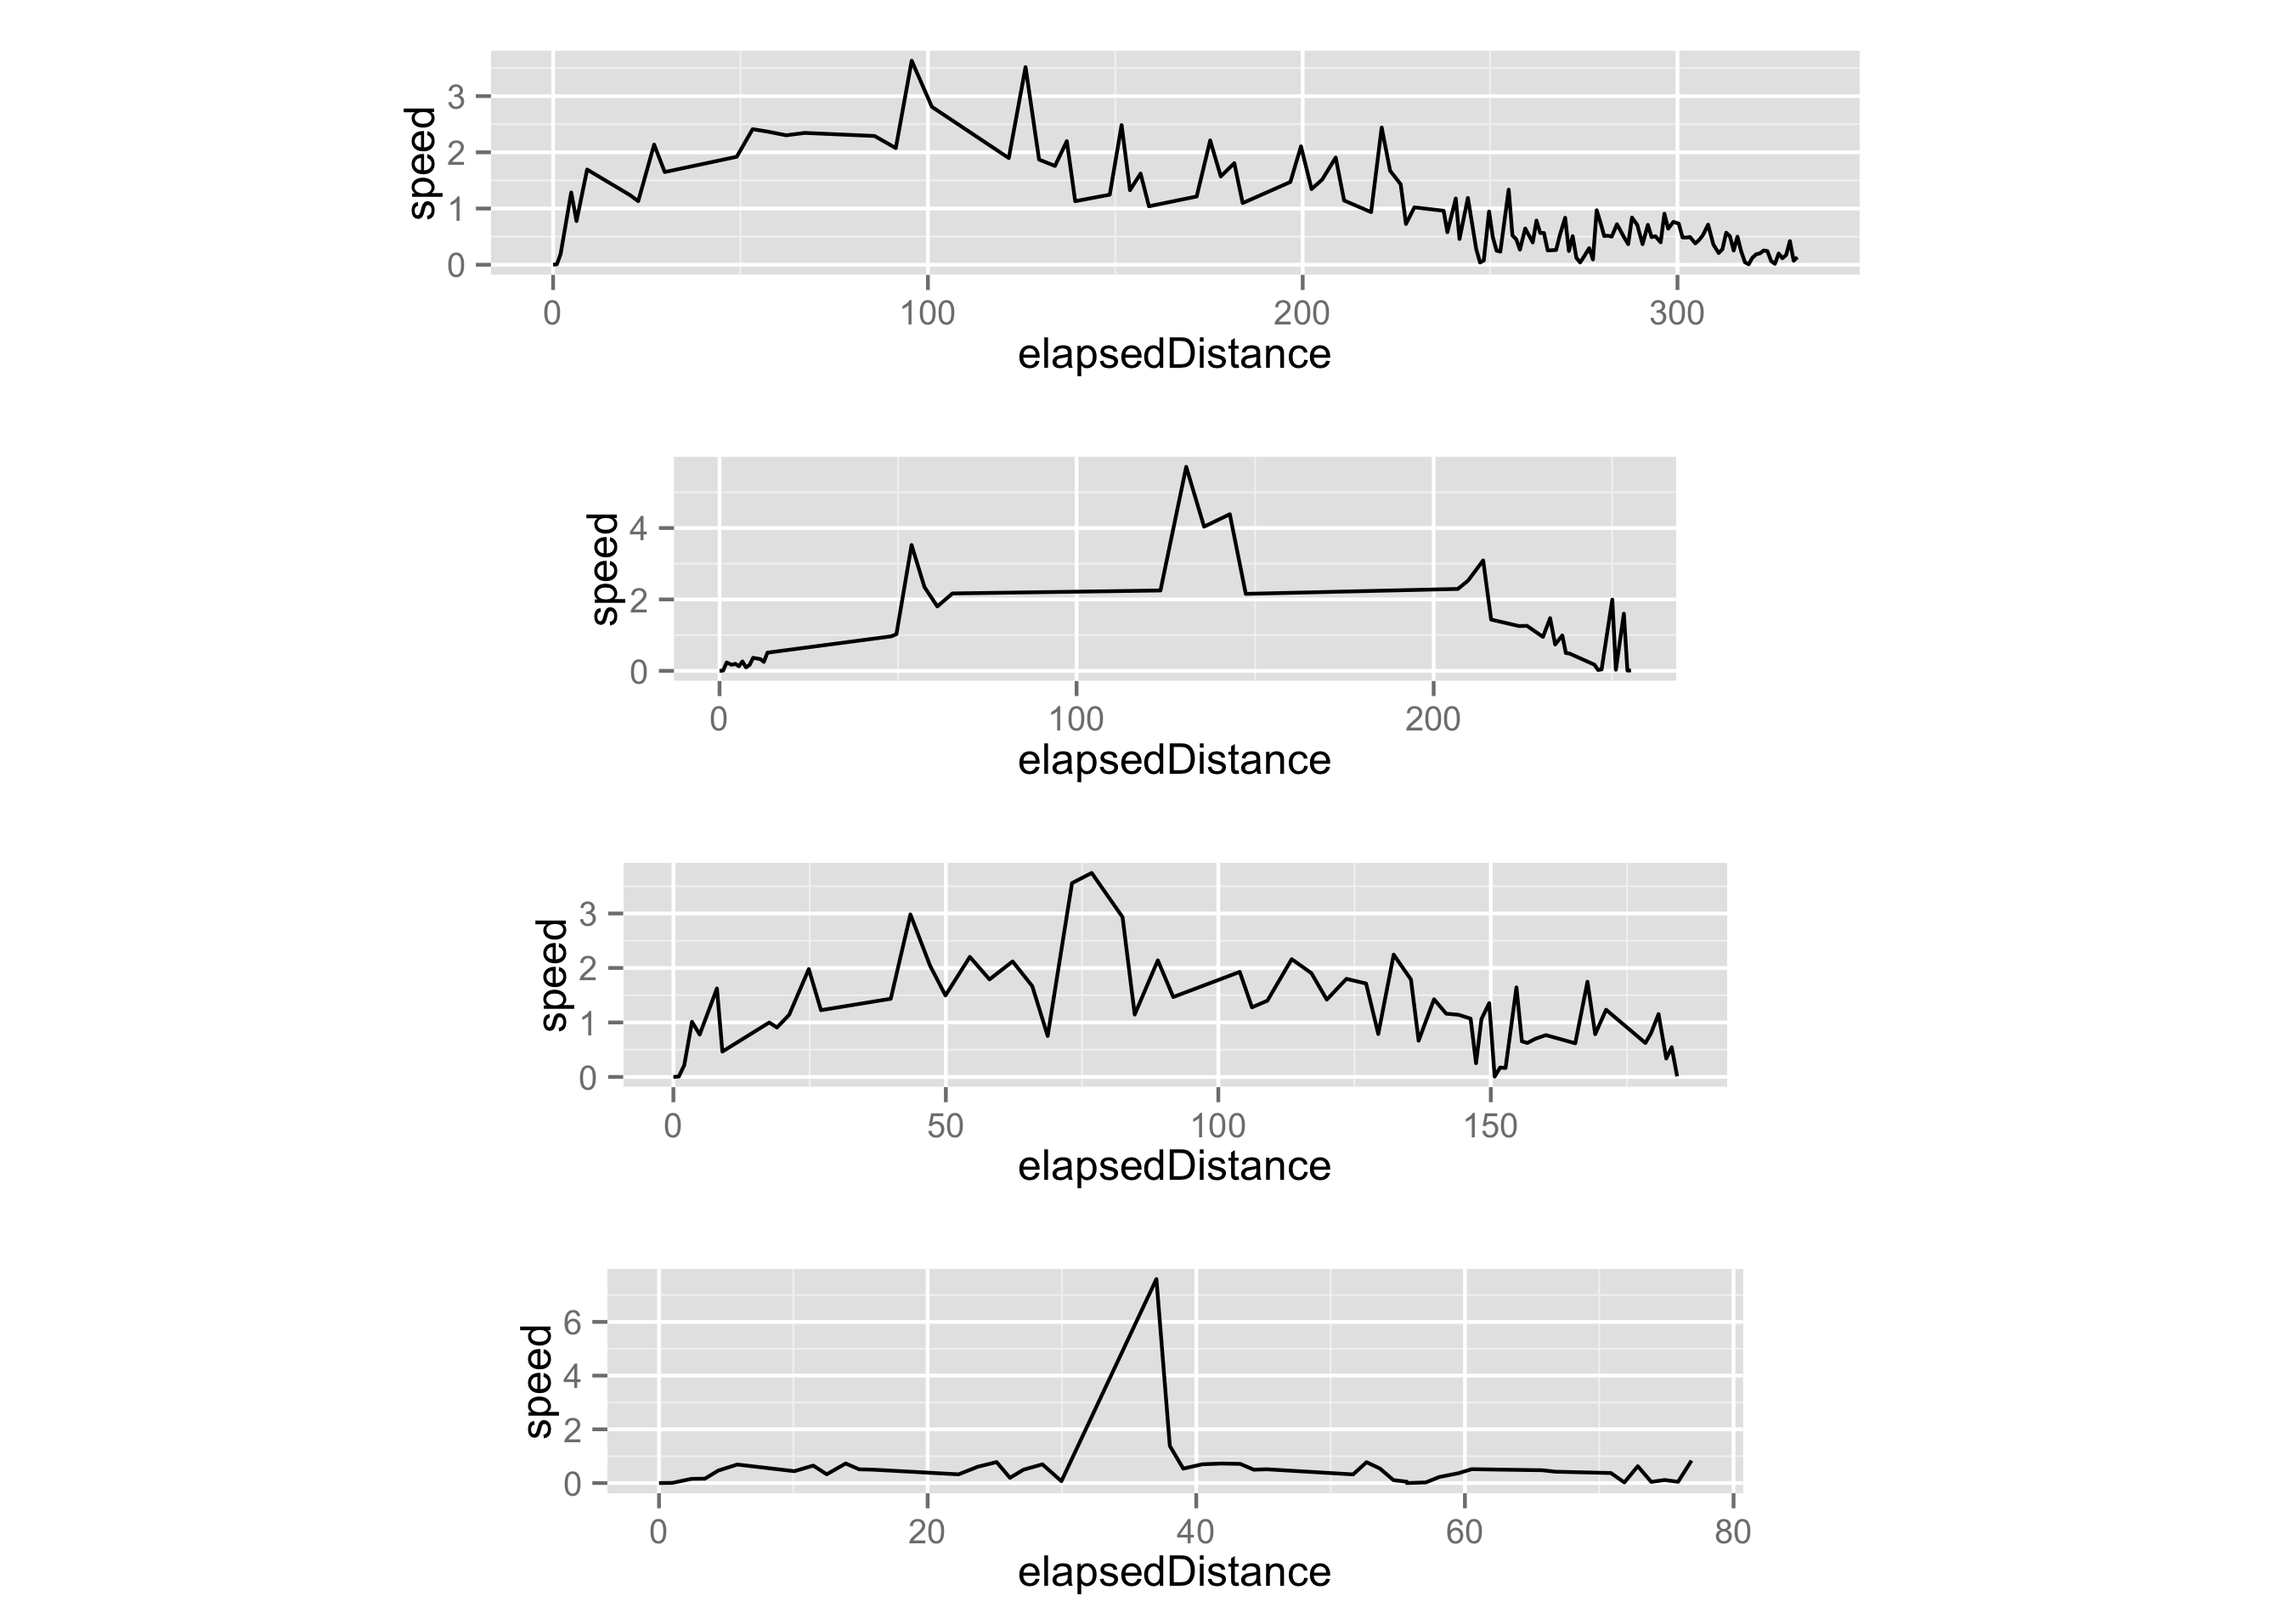
\includegraphics[width=\linewidth]{images/plots/plot_speed_individual_45}
		\captionof{figure}{Fartprofiler for testdeltager 45's opgave 20,23,8 og 20. Den tilbagelagte distance ud af $x$-aksen og farten ud af $y$-aksen}
	\end{minipage}
		\begin{minipage}{0.5\linewidth}
		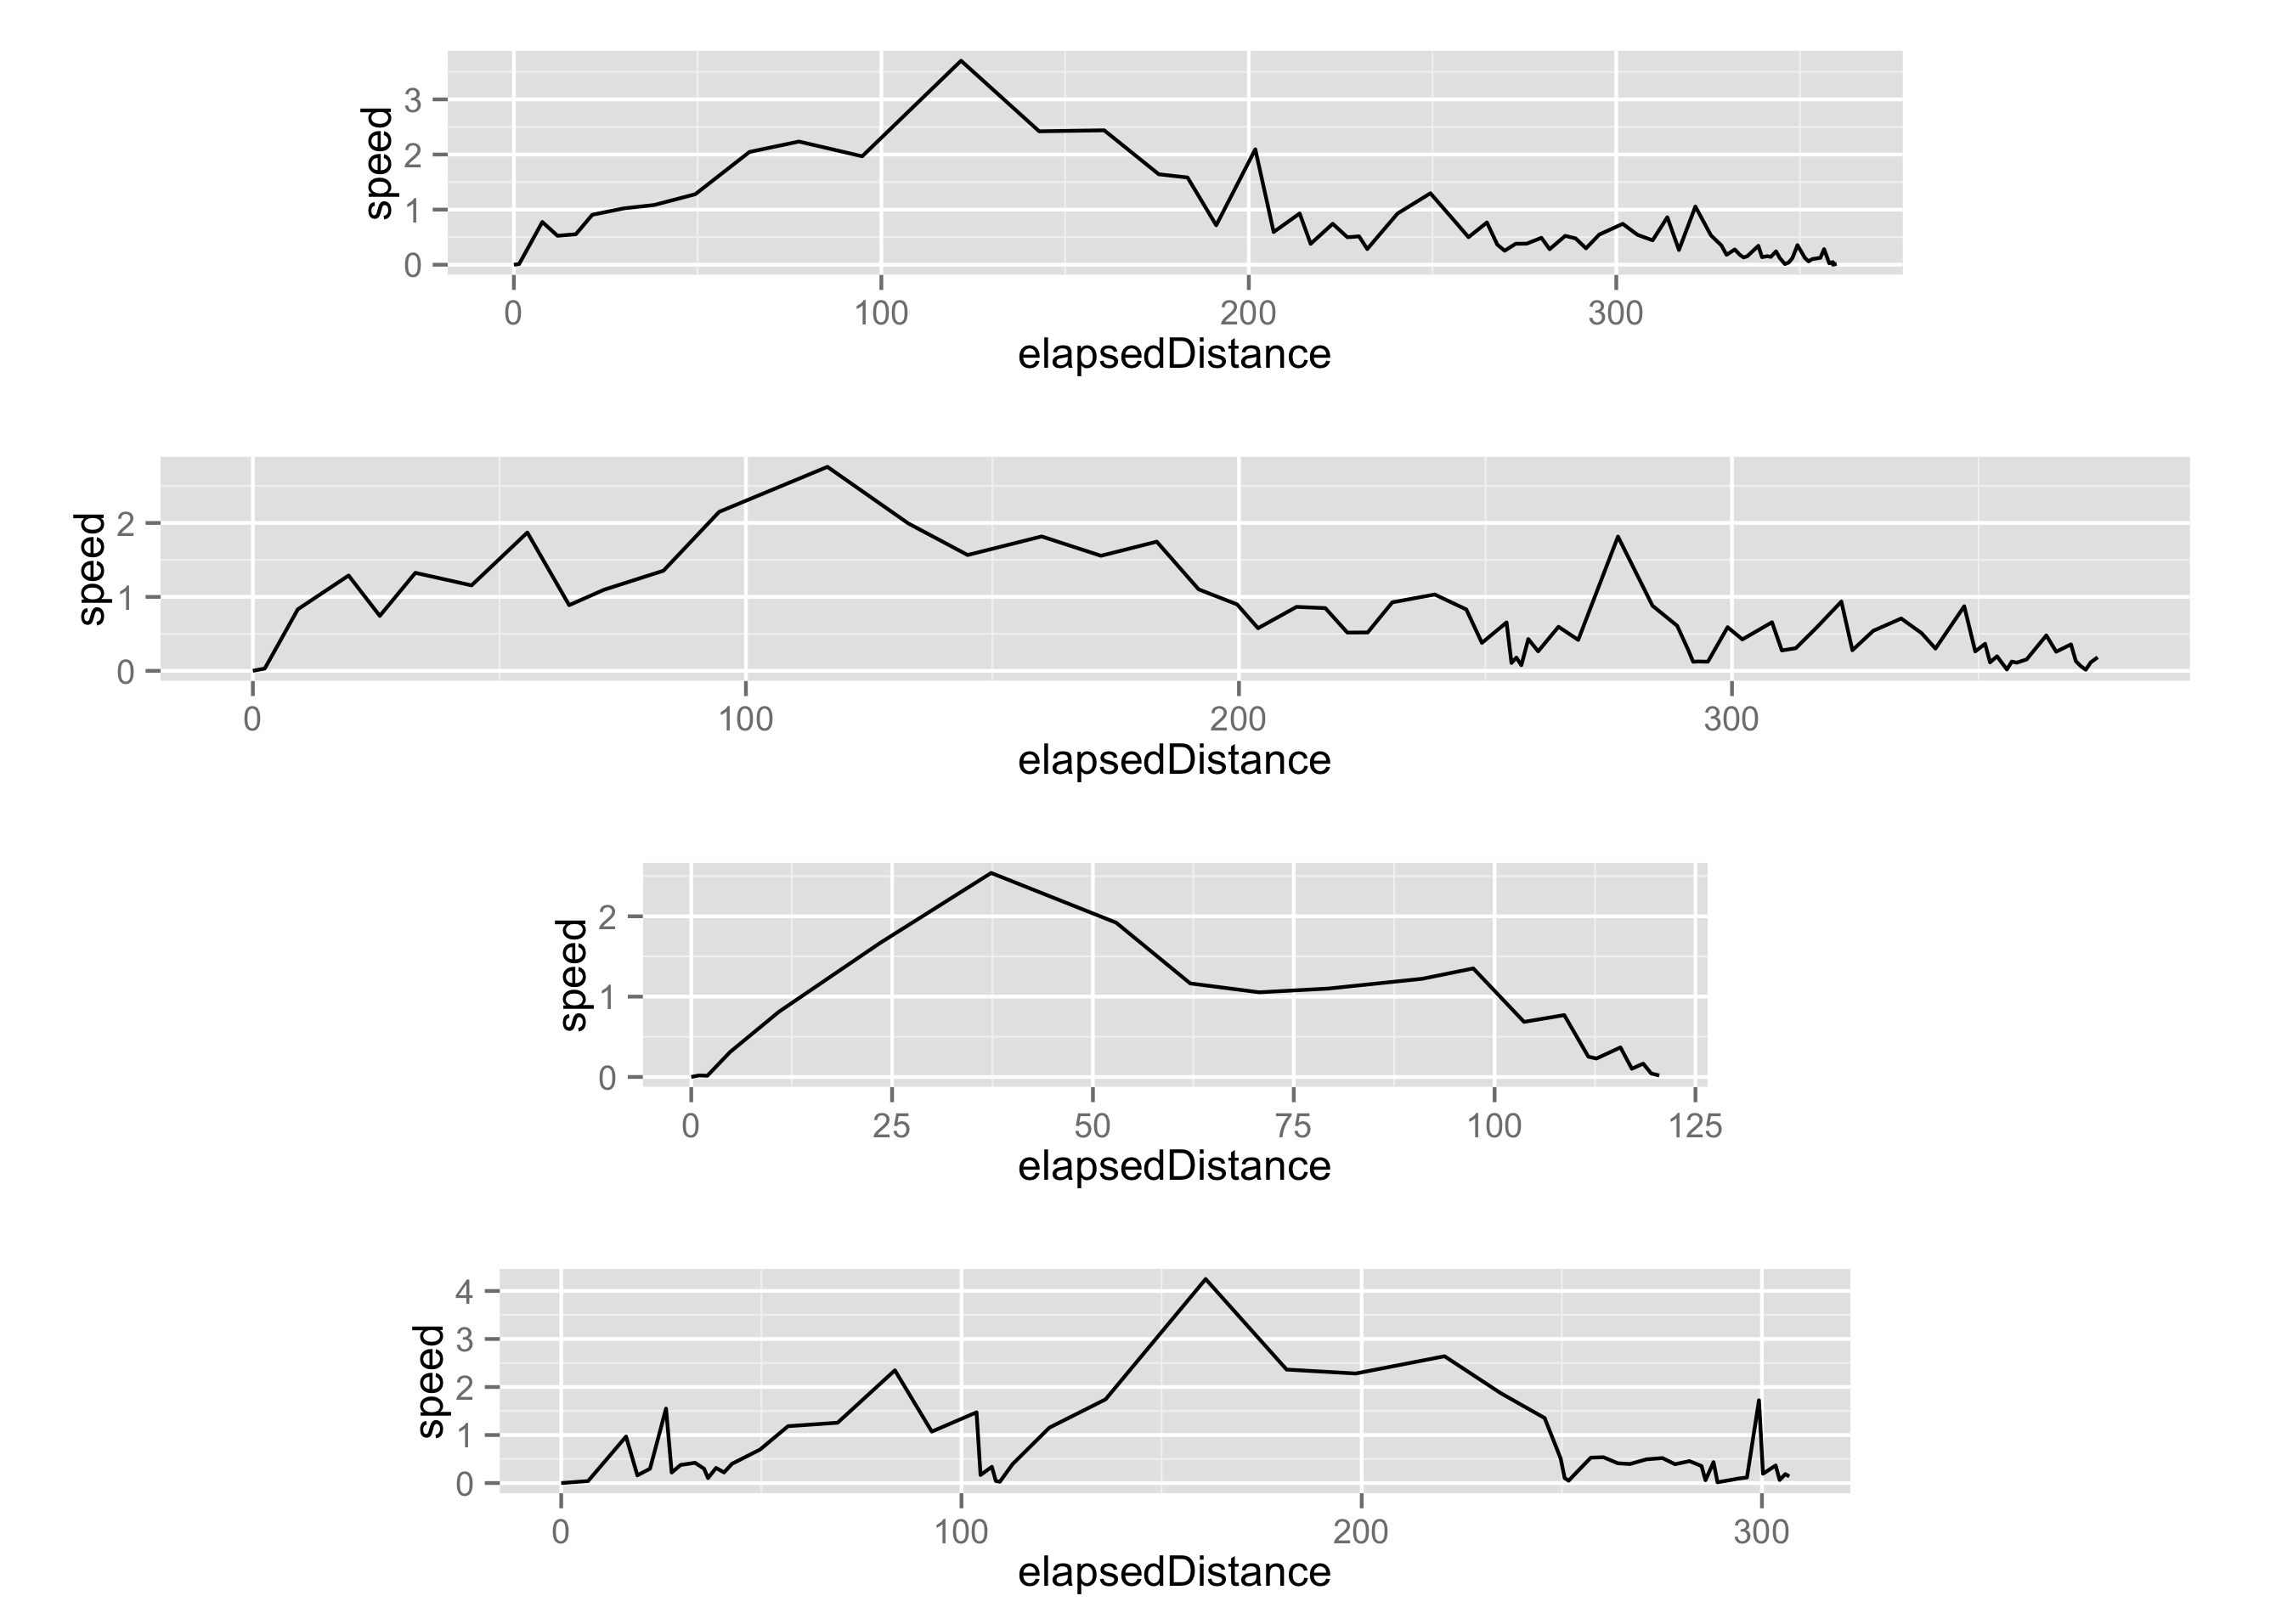
\includegraphics[width=\linewidth]{images/plots/plot_speed_individual_77}
		\captionof{figure}{Fartprofiler for testdeltager 77's opgave 20,23,8 og 20. Den tilbagelagte distance ud af $x$-aksen og farten ud af $y$-aksen}
	\end{minipage}
	\begin{minipage}{0.5\linewidth}
		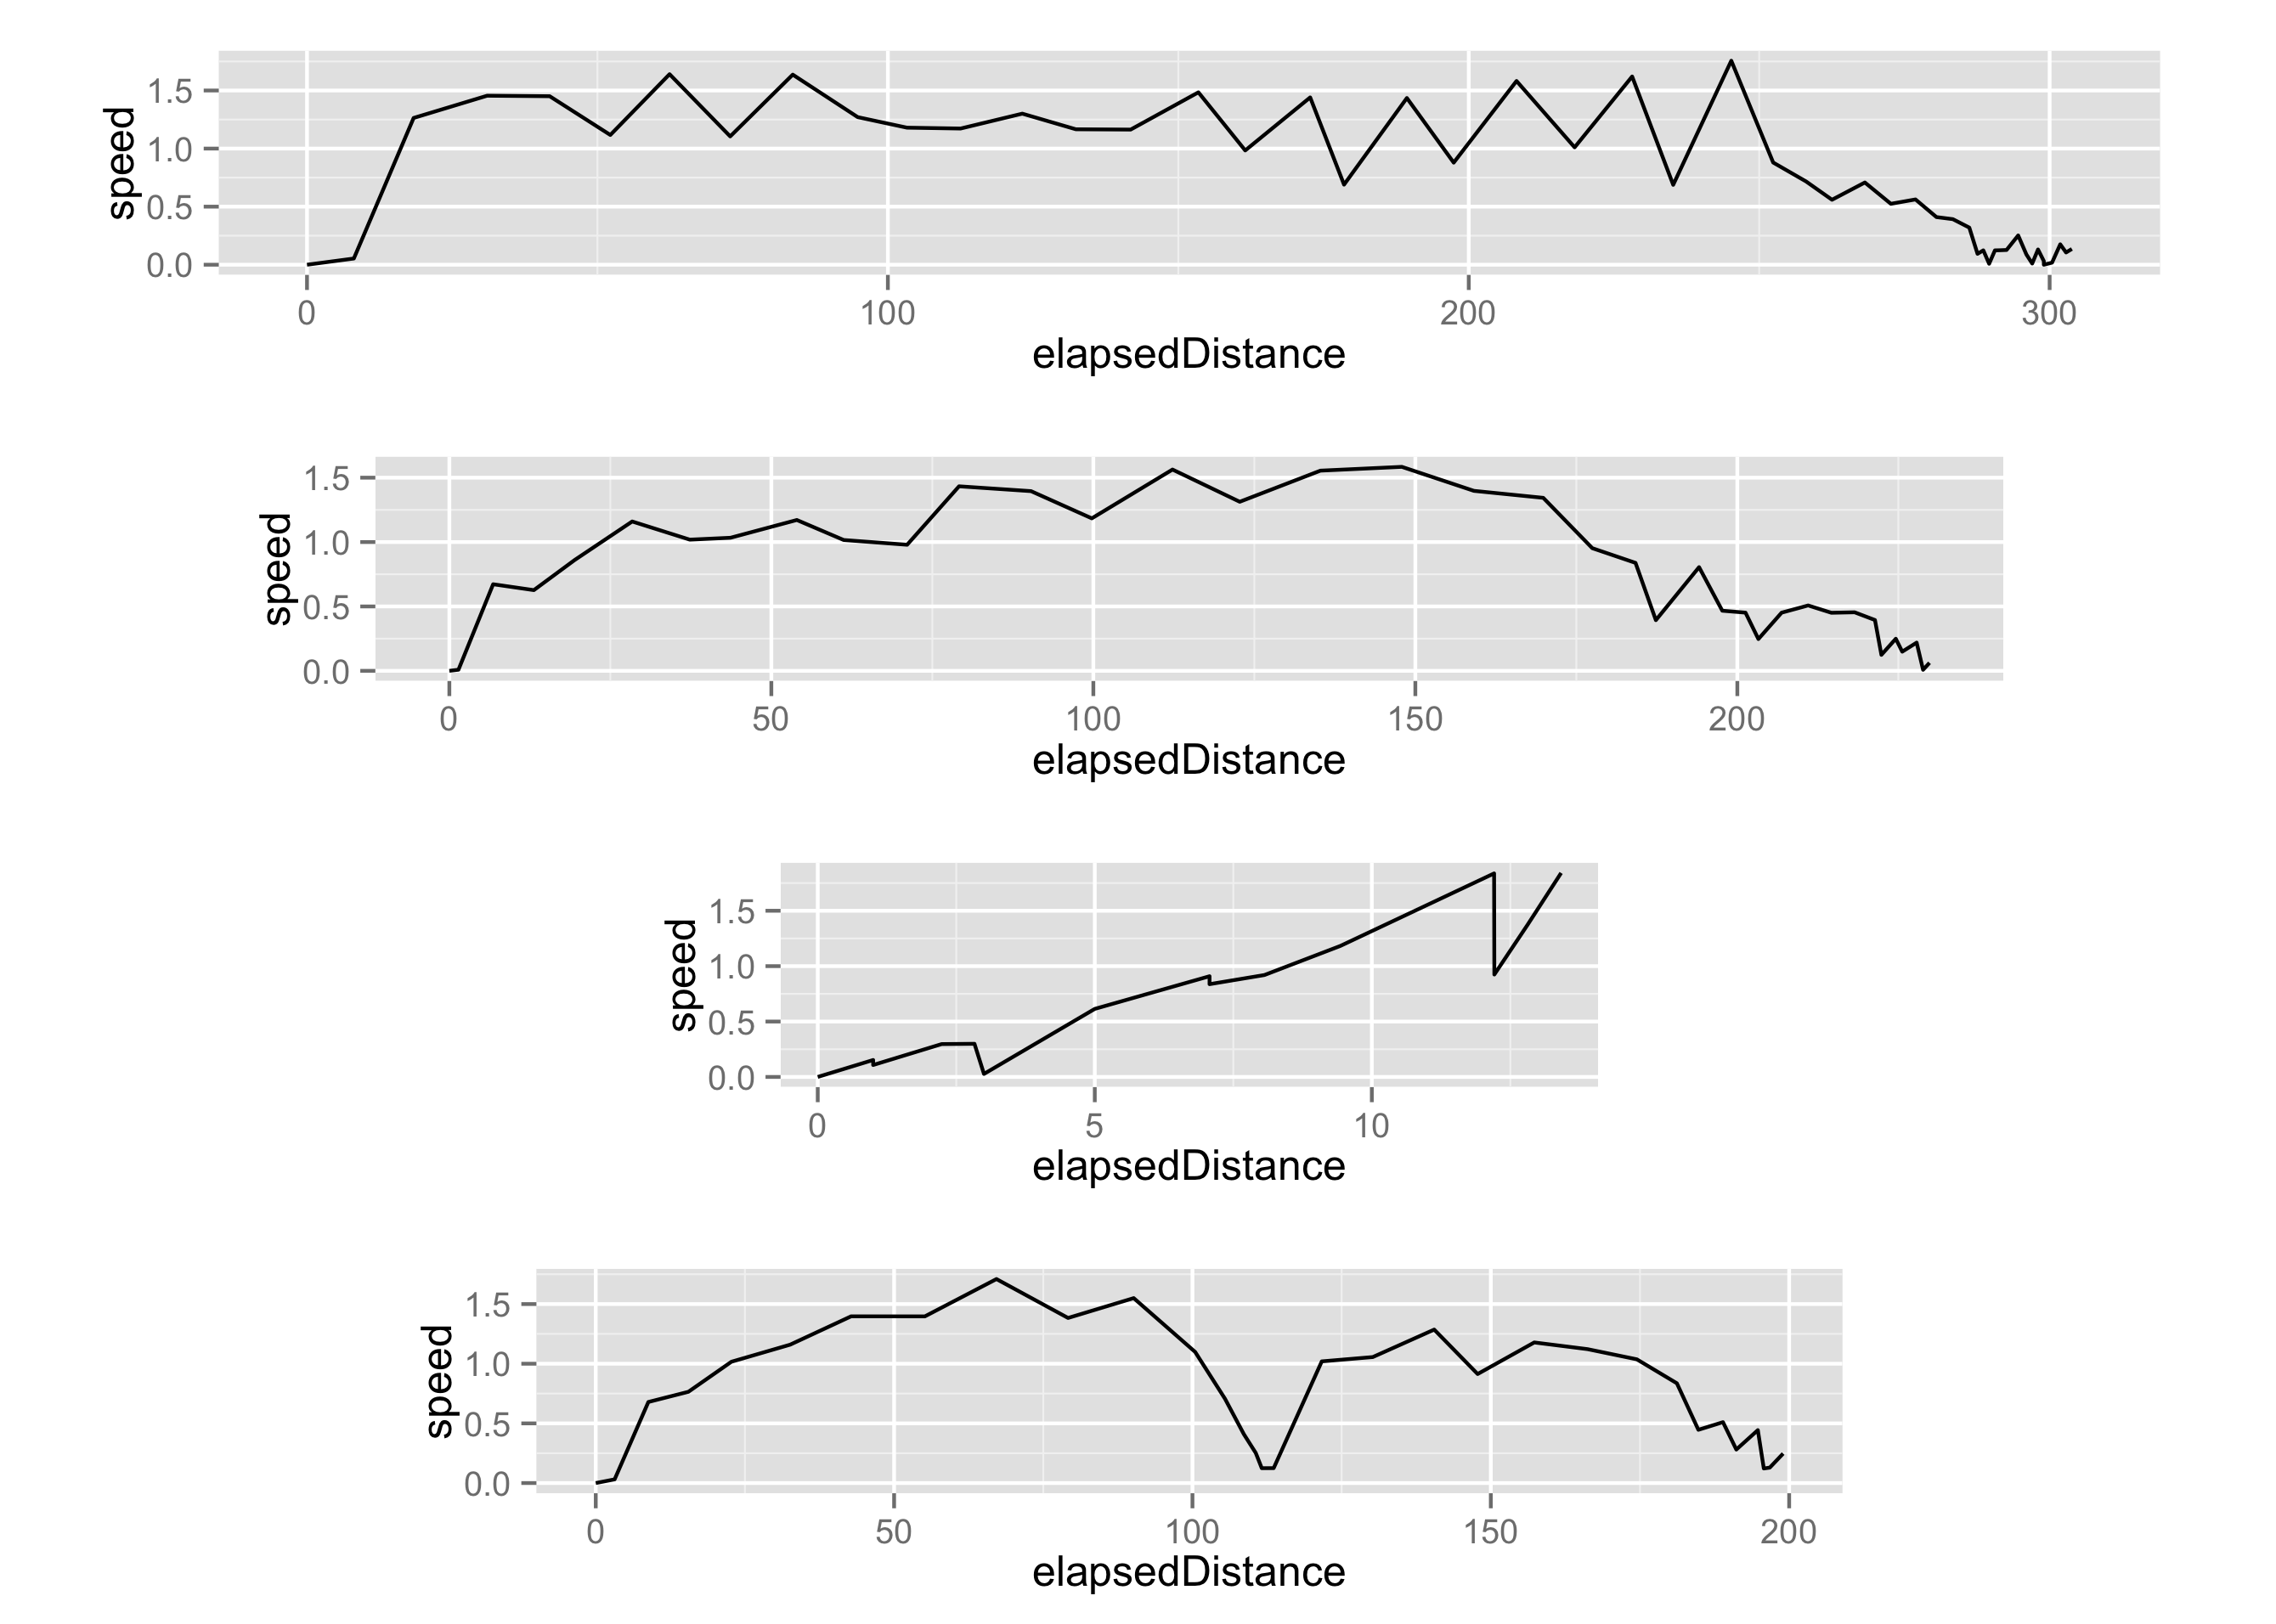
\includegraphics[width=\linewidth]{images/plots/plot_speed_individual_113}
		\captionof{figure}{Fartprofiler for testdeltager 113's opgave 20,23,8 og 20. Den tilbagelagte distance ud af $x$-aksen og farten ud af $y$-aksen}
	\end{minipage}
	\begin{minipage}{0.5\linewidth}
		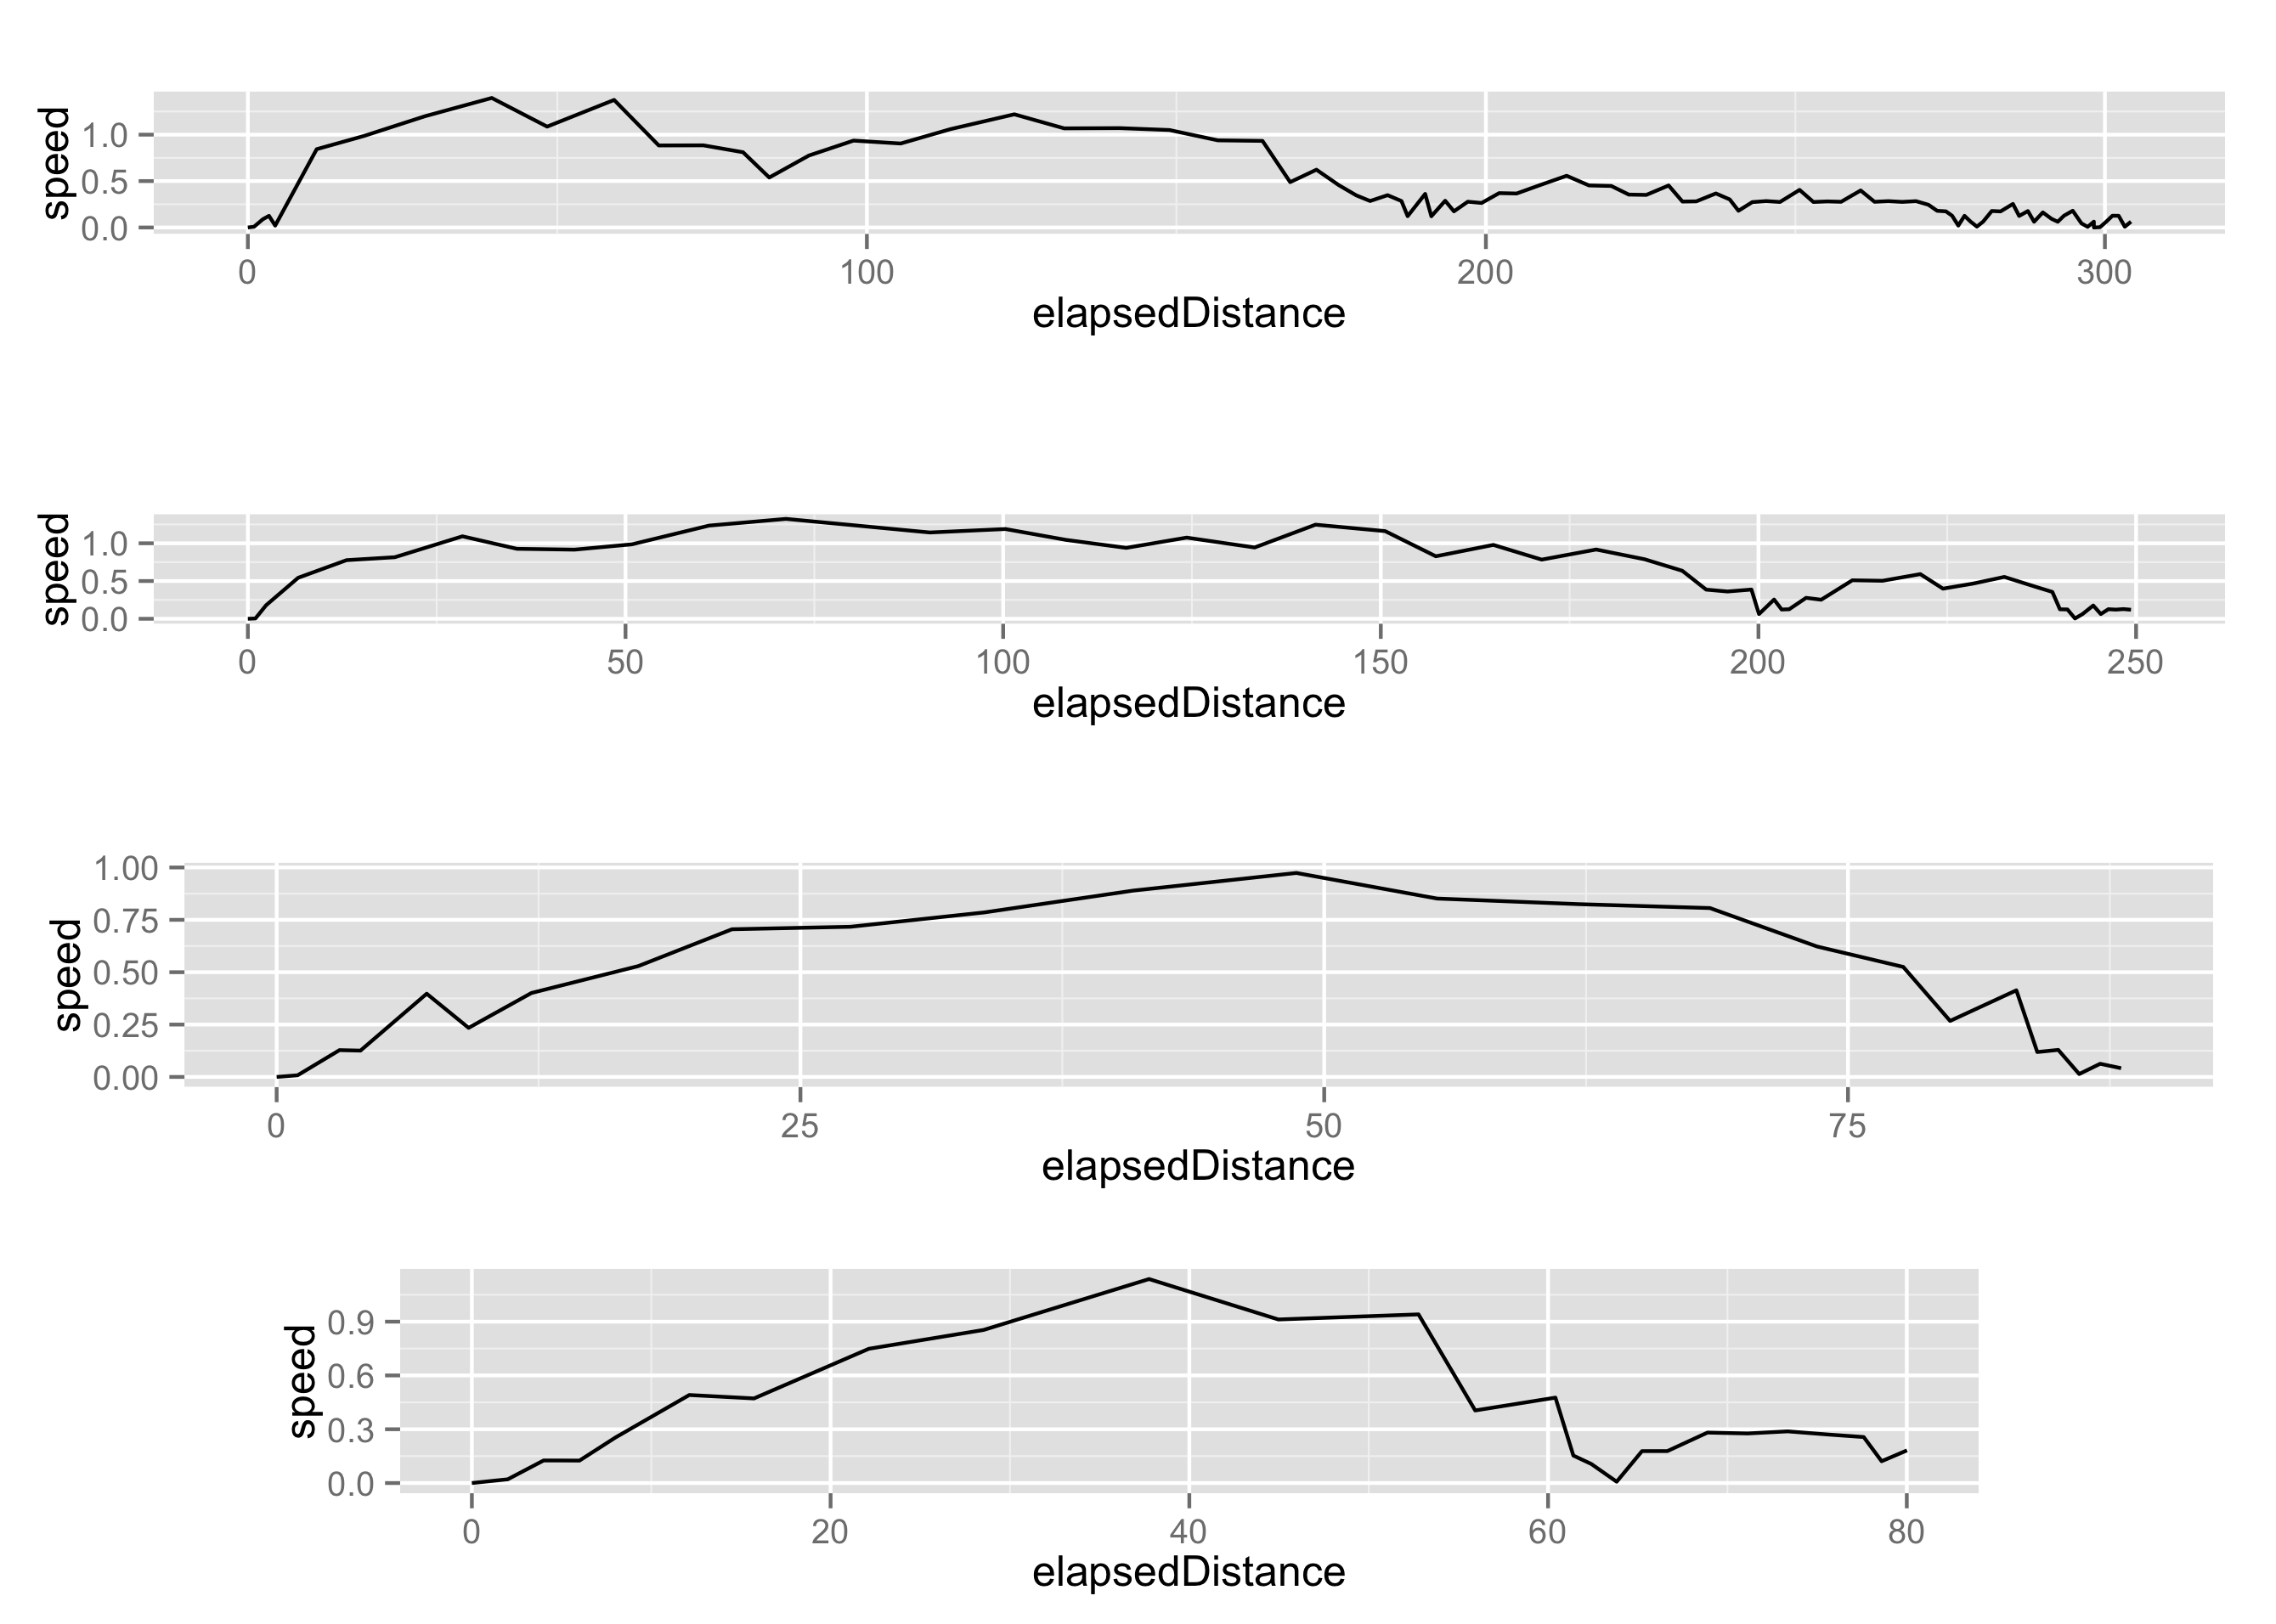
\includegraphics[width=\linewidth]{images/plots/plot_speed_individual_161}
		\captionof{figure}{Fartprofiler for testdeltager 161's opgave 20,23,8 og 20. Den tilbagelagte distance ud af $x$-aksen og farten ud af $y$-aksen}
	\end{minipage}
	\label{fig:kvaliativ_persons_3}
\end{minipage}

\begin{minipage}{\textwidth}
	\begin{minipage}{0.5\linewidth}
		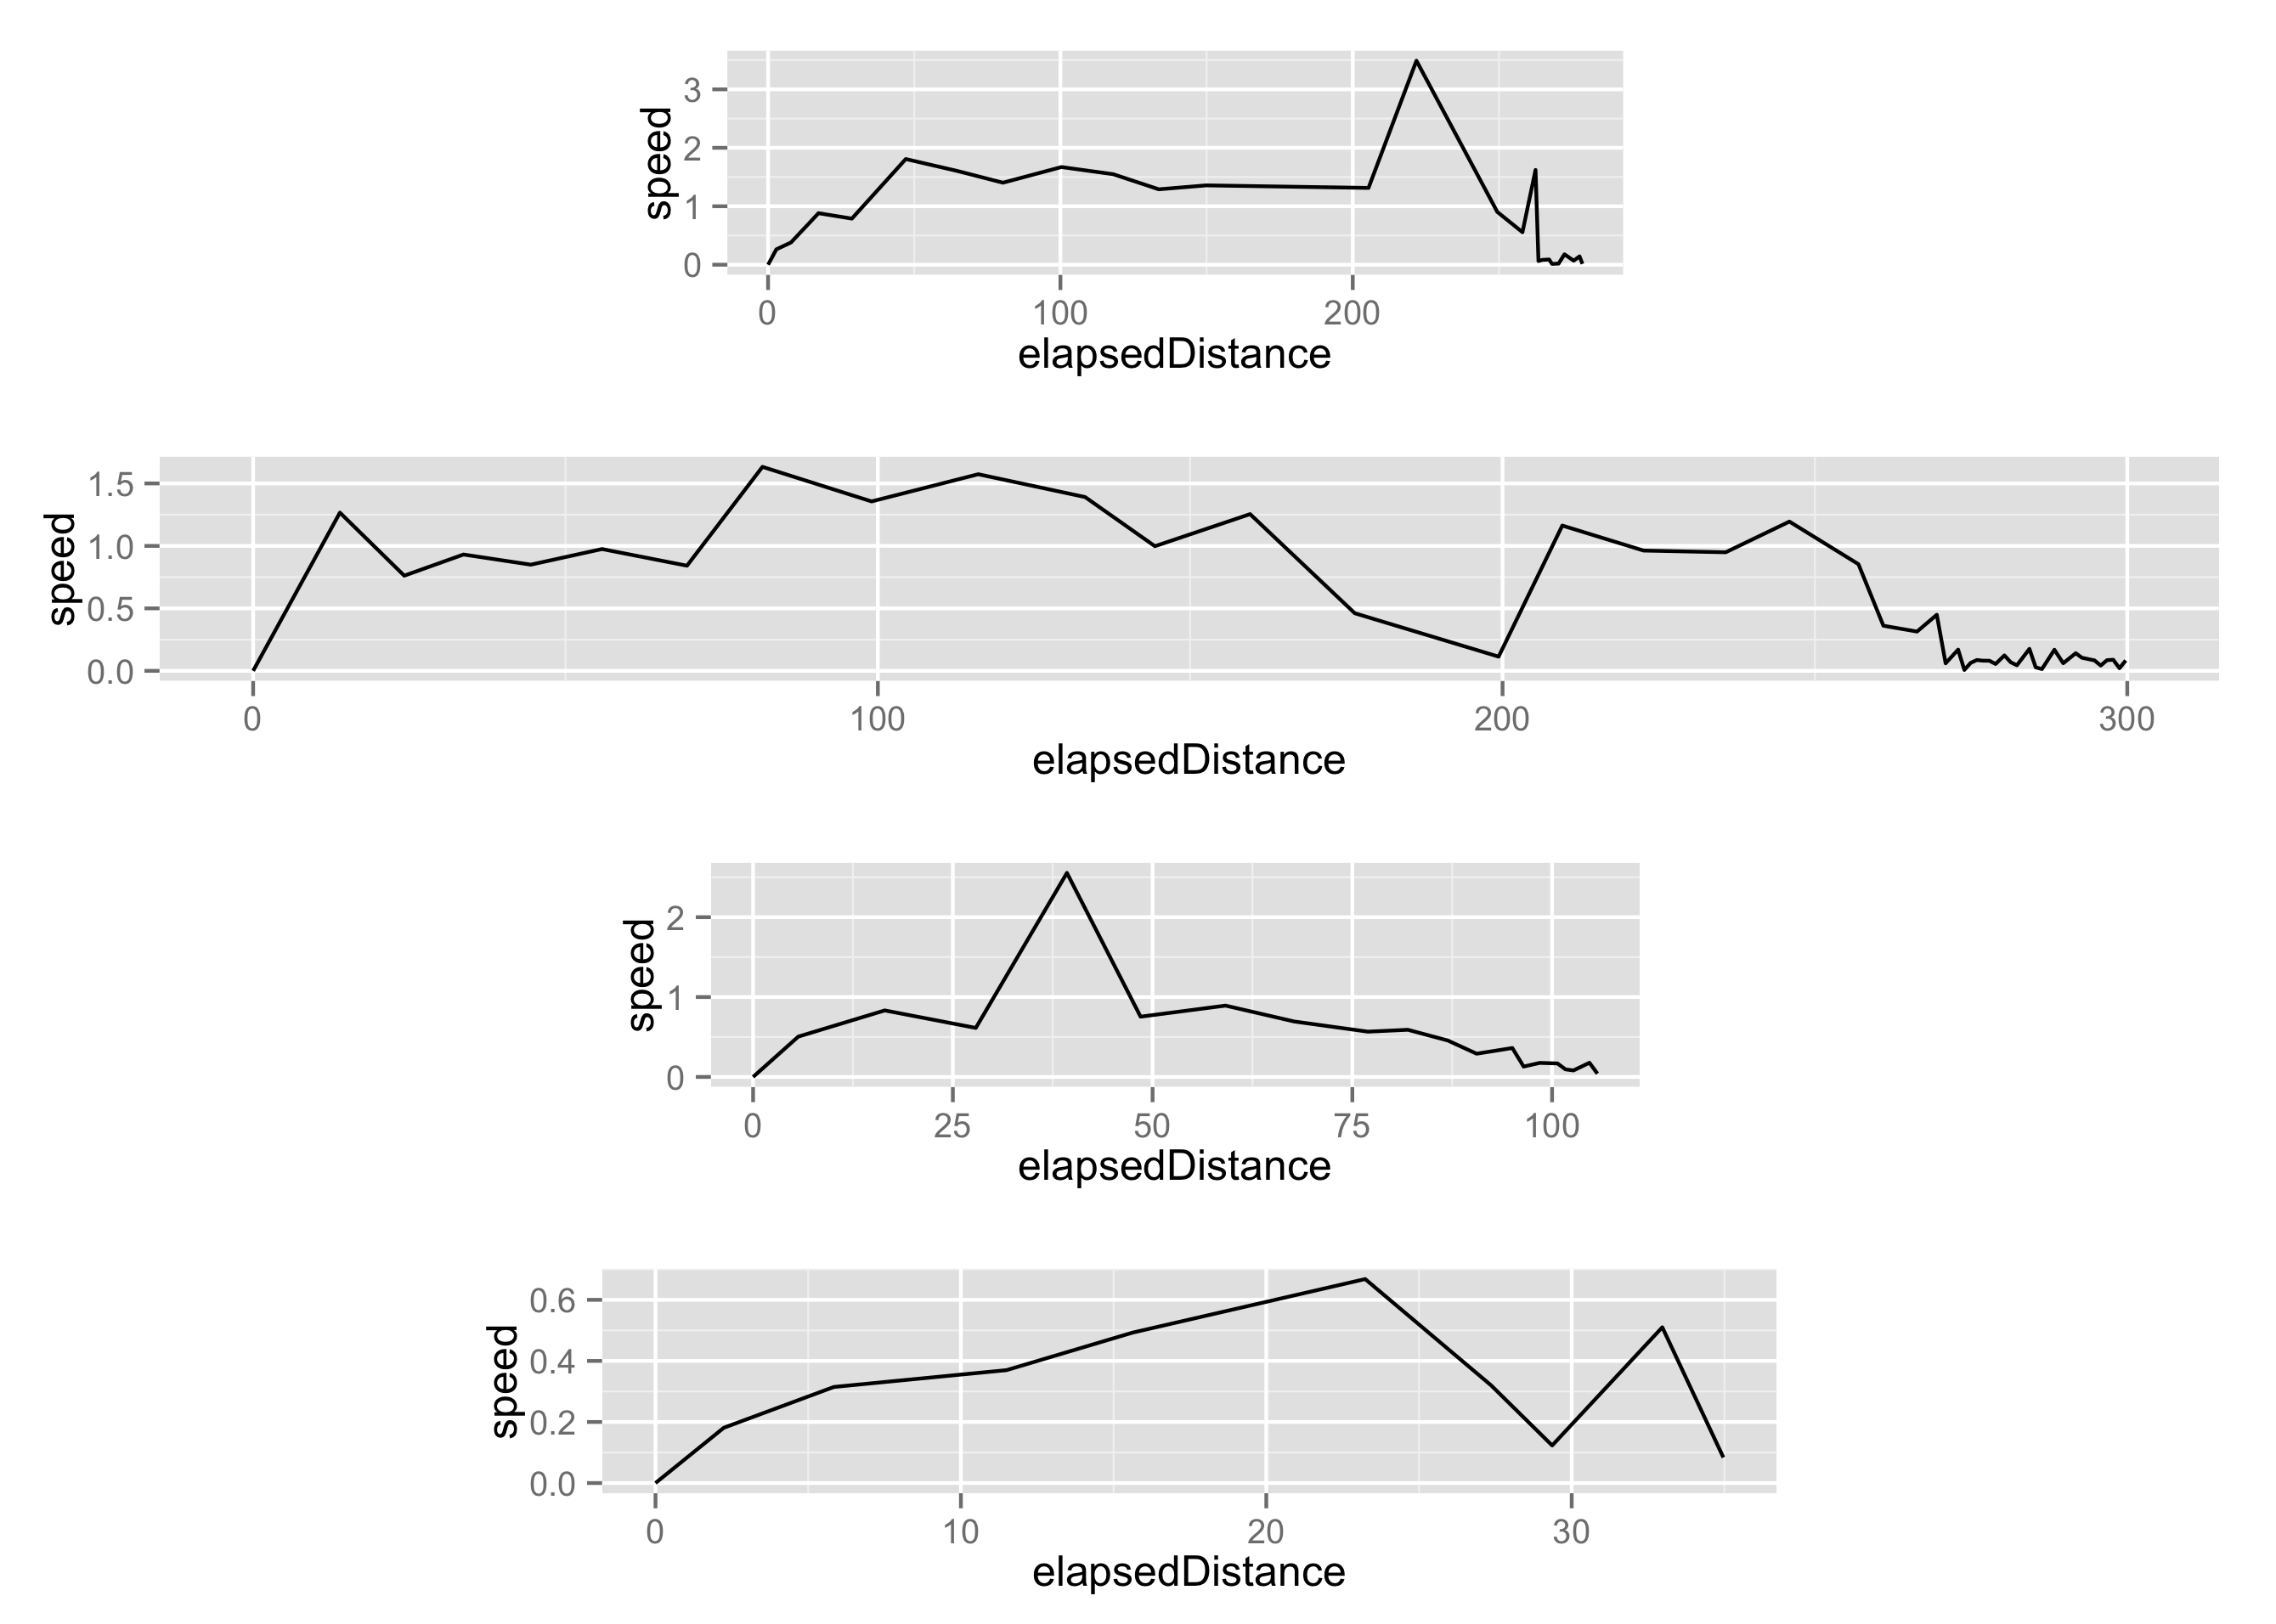
\includegraphics[width=\linewidth]{images/plots/plot_speed_individual_166}
		\captionof{figure}{Fartprofiler for testdeltager 168's opgave 20,23,8 og 20. Den tilbagelagte distance ud af $x$-aksen og farten ud af $y$-aksen}
	\end{minipage}
		\begin{minipage}{0.5\linewidth}
		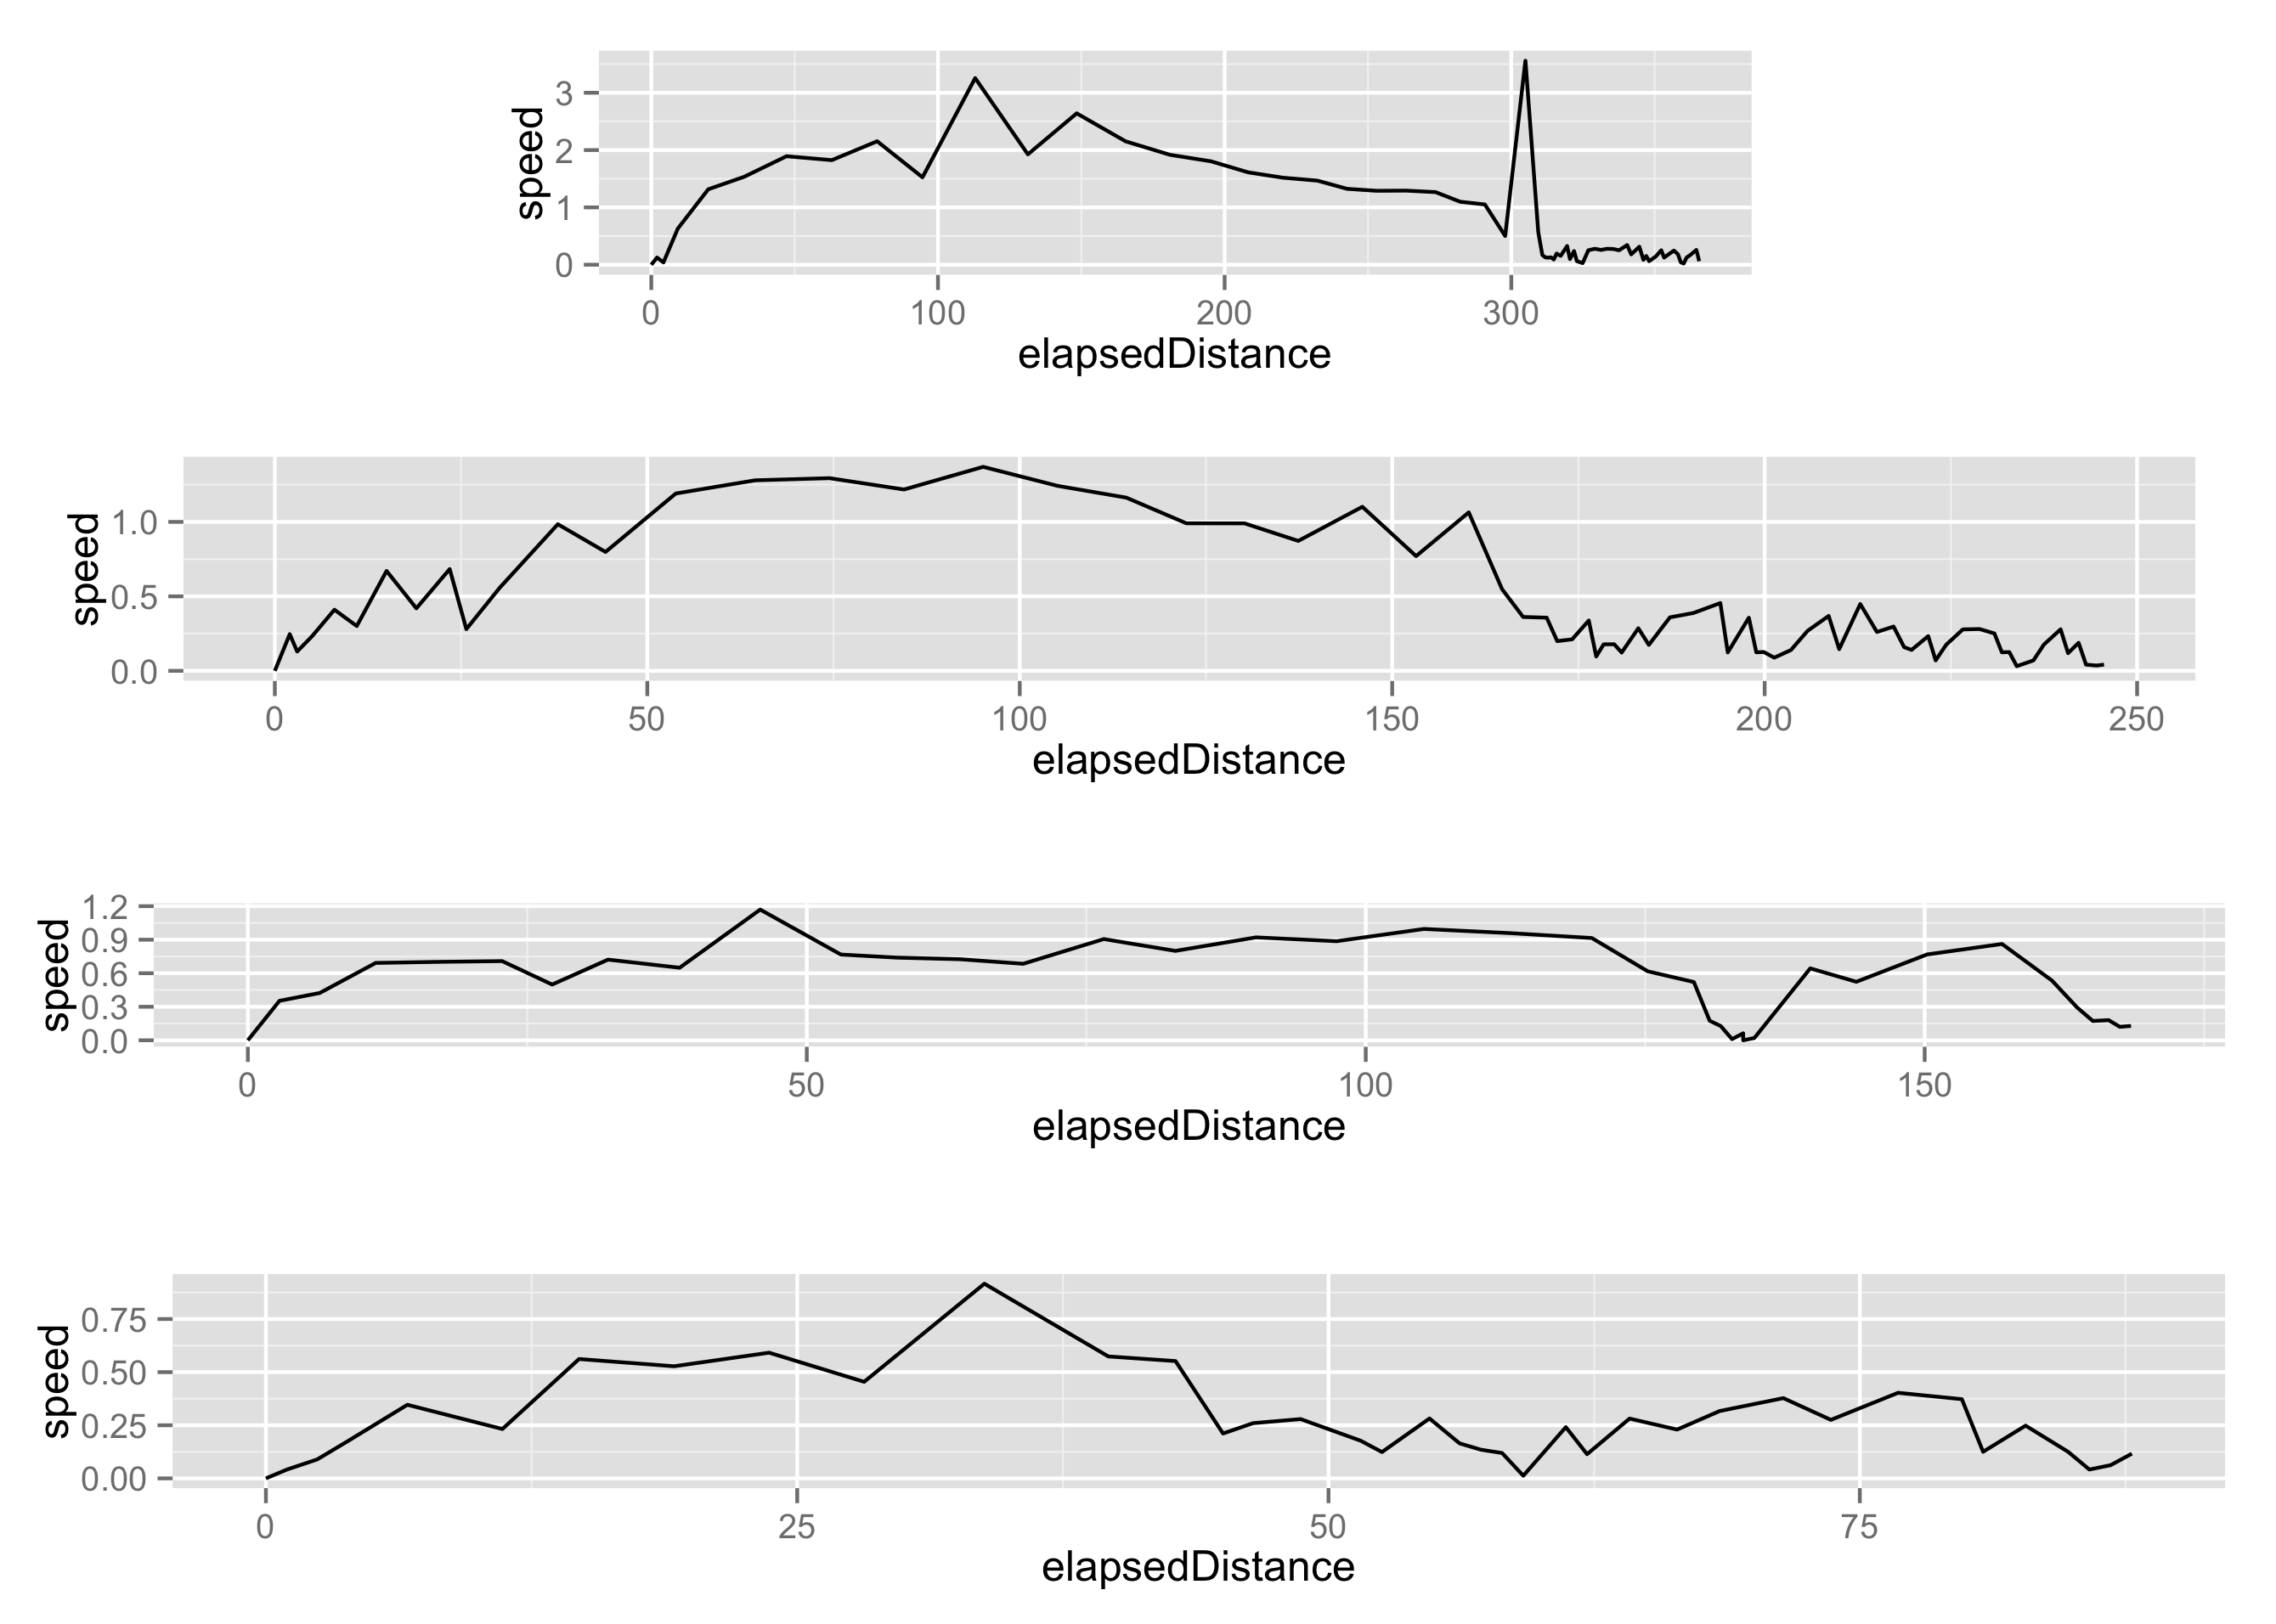
\includegraphics[width=\linewidth]{images/plots/plot_speed_individual_226}
		\captionof{figure}{Fartprofiler for testdeltager 226's opgave 20,23,8 og 20. Den tilbagelagte distance ud af $x$-aksen og farten ud af $y$-aksen}
	\end{minipage}
	\begin{minipage}{0.5\linewidth}
		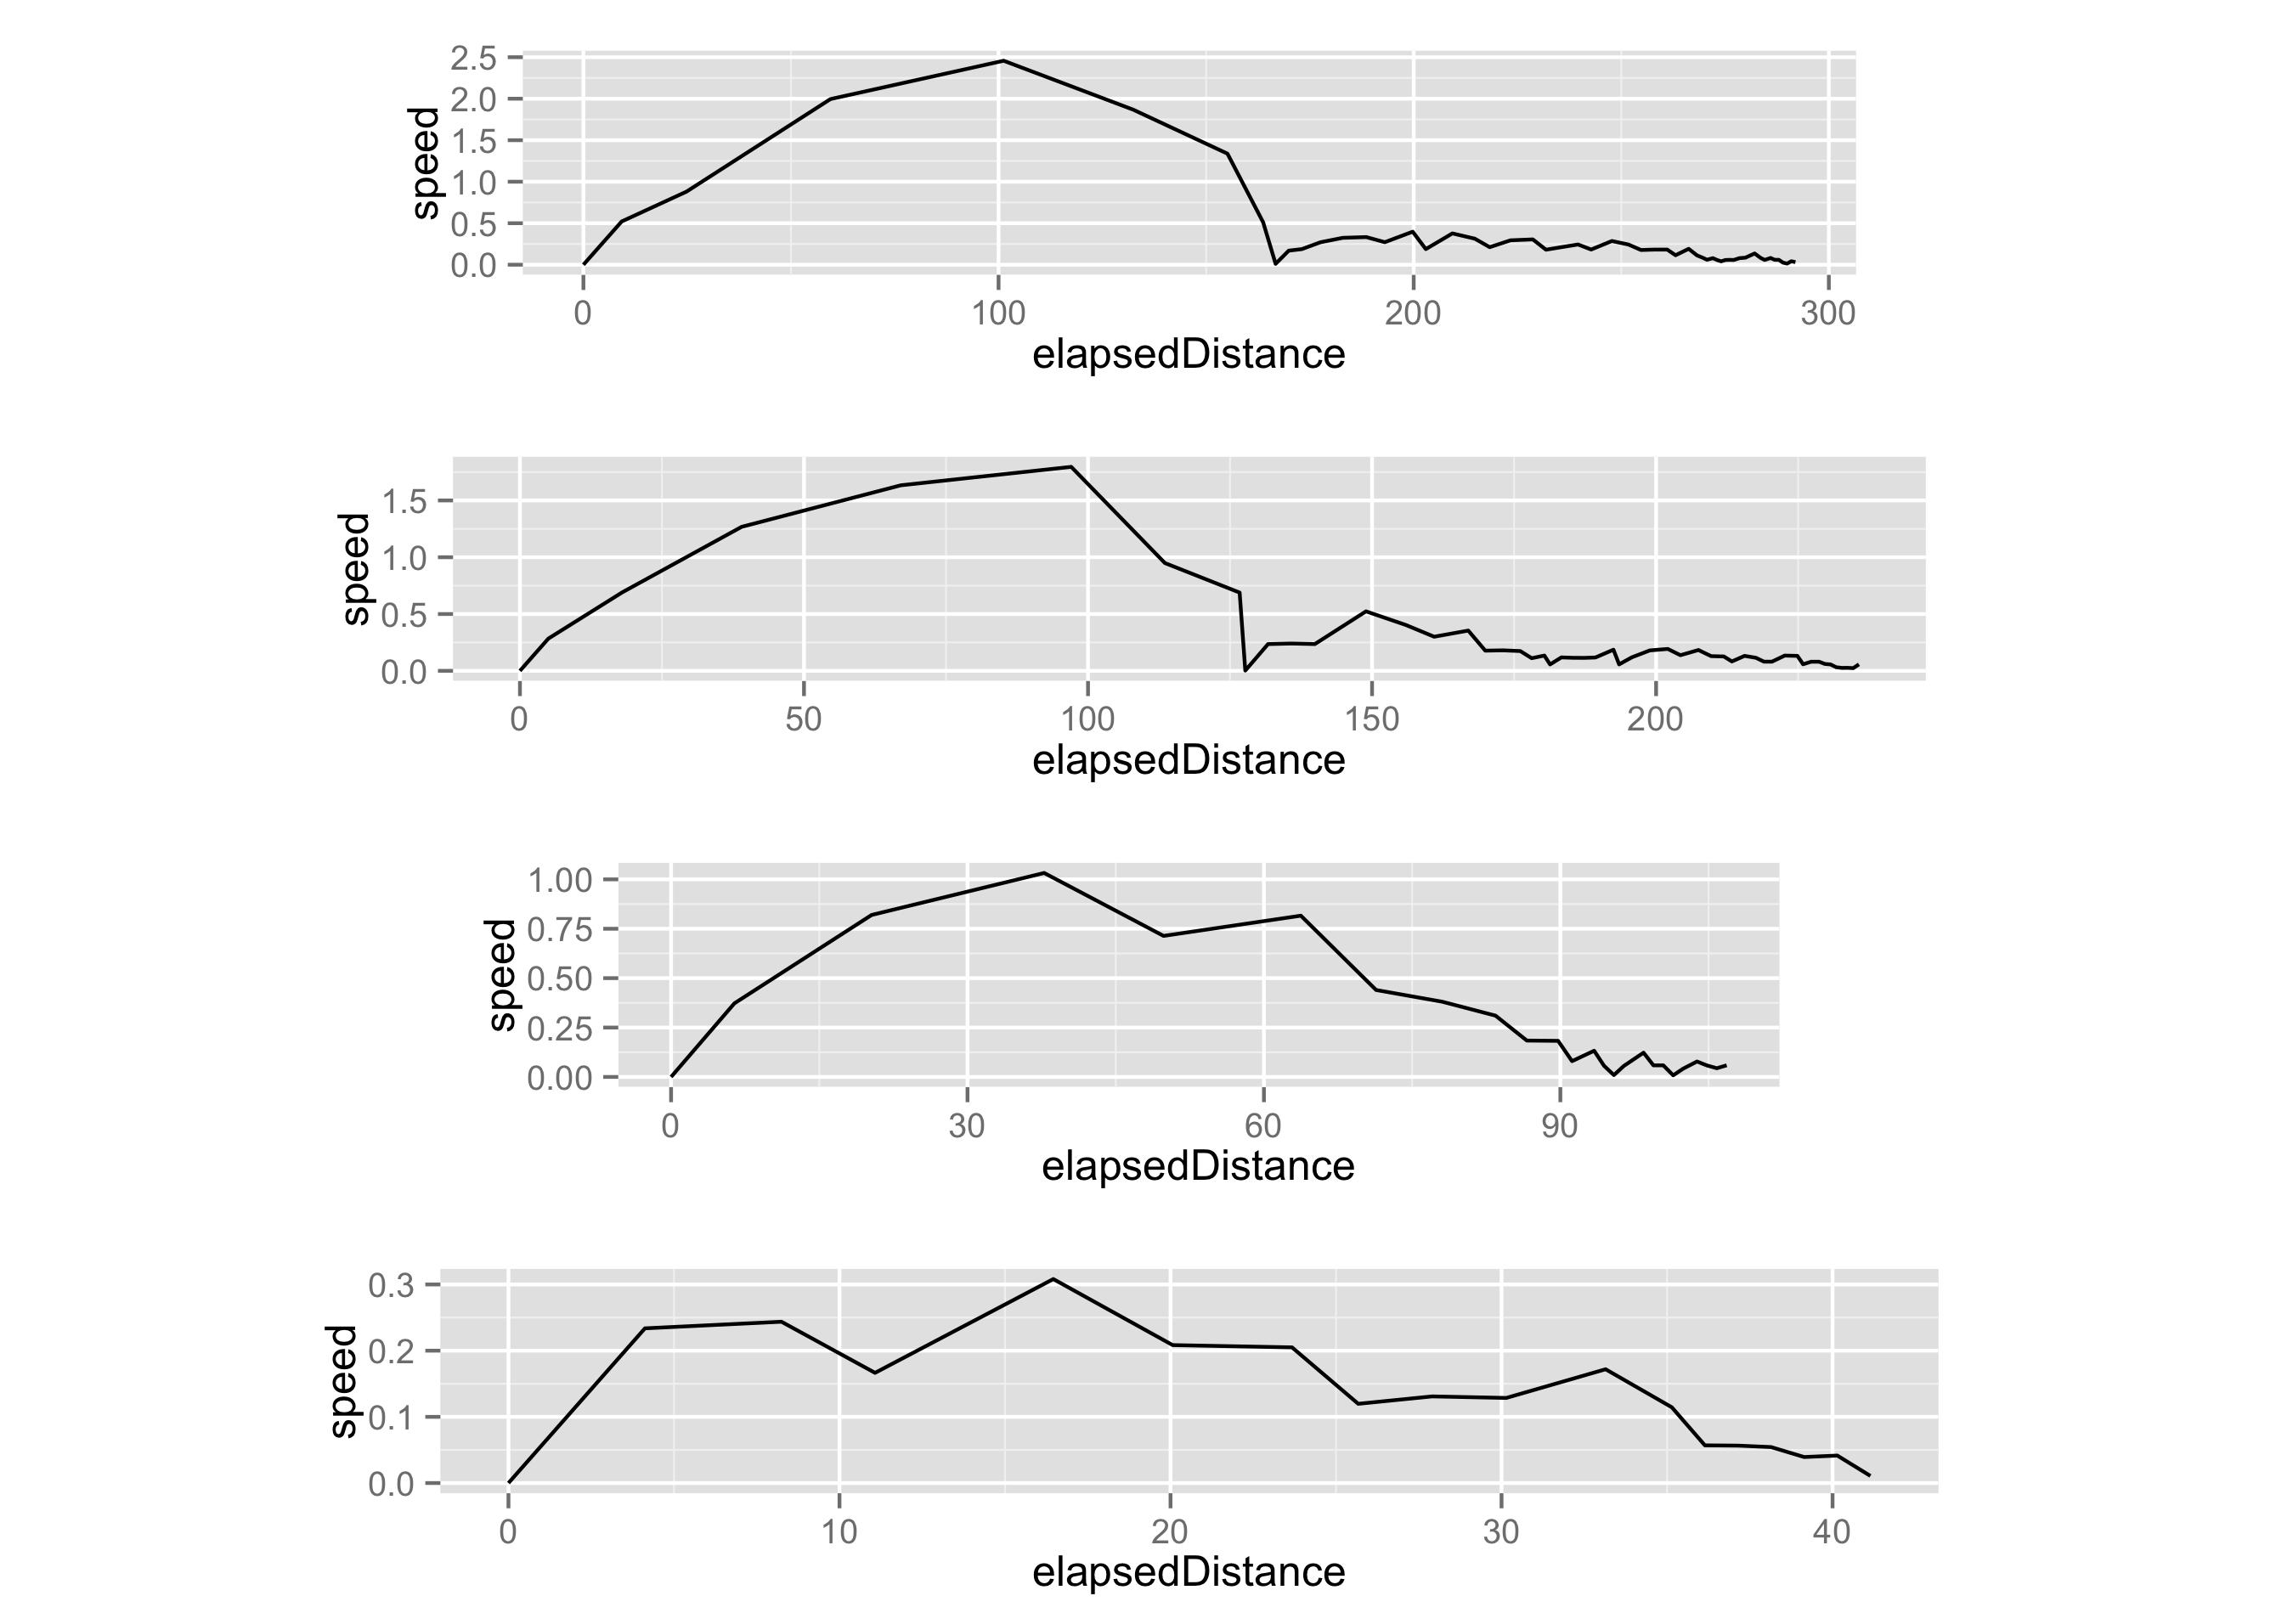
\includegraphics[width=\linewidth]{images/plots/plot_speed_individual_239}
		\captionof{figure}{Fartprofiler for testdeltager 239's opgave 20,23,8 og 20. Den tilbagelagte distance ud af $x$-aksen og farten ud af $y$-aksen}
	\end{minipage}
	\begin{minipage}{0.5\linewidth}
		\includegraphics[width=\linewidth]{images/plots/plot_speed_individual_263}
		\captionof{figure}{Fartprofiler for testdeltager 263's opgave 20,23,8 og 20. Den tilbagelagte distance ud af $x$-aksen og farten ud af $y$-aksen}
	\end{minipage}
	\captionof{figure}{Fartprofiler for testdeltager 166,225,239 og 263's opgave 20,23,8 og 20. Den tilbagelagte distance ud af $x$-aksen og farten ud af $y$-aksen}
	\label{fig:kvaliativ_persons_3}
\end{minipage}

\begin{minipage}{\textwidth}
	\begin{minipage}{0.5\linewidth}
		\includegraphics[width=\linewidth]{images/plots/plot_speed_time_individual_45}
		\captionof{figure}{Fartprofiler for testdeltager 45's opgave 20,23,8 og 20. Den forløbne tid ud af $x$-aksen og farten ud af $y$-aksen}
	\end{minipage}
		\begin{minipage}{0.5\linewidth}
		\includegraphics[width=\linewidth]{images/plots/plot_speed_time_individual_77}
		\captionof{figure}{Fartprofiler for testdeltager 77's opgave 20,23,8 og 20. Den forløbne tid ud af $x$-aksen og farten ud af $y$-aksen}
	\end{minipage}
	\begin{minipage}{0.5\linewidth}
		\includegraphics[width=\linewidth]{images/plots/plot_speed_time_individual_113}
		\captionof{figure}{Fartprofiler for testdeltager 113's opgave 20,23,8 og 20. Den forløbne tid ud af $x$-aksen og farten ud af $y$-aksen}
	\end{minipage}
	\begin{minipage}{0.5\linewidth}
		\includegraphics[width=\linewidth]{images/plots/plot_speed_time_individual_161}
		\captionof{figure}{Fartprofiler for testdeltager 161's opgave 20,23,8 og 20. Den forløbne tid ud af $x$-aksen og farten ud af $y$-aksen}
	\end{minipage}
	\label{fig:kvaliativ_persons_3}
\end{minipage}

\begin{minipage}{\textwidth}
	\begin{minipage}{0.5\linewidth}
		\includegraphics[width=\linewidth]{images/plots/plot_speed_time_individual_166}
		\captionof{figure}{Fartprofiler for testdeltager 166's opgave 20,23,8 og 20. Den forløbne tid ud af $x$-aksen og farten ud af $y$-aksen}
	\end{minipage}
		\begin{minipage}{0.5\linewidth}
		\includegraphics[width=\linewidth]{images/plots/plot_speed_time_individual_226}
		\captionof{figure}{Fartprofiler for testdeltager 226's opgave 20,23,8 og 20. Den forløbne tid ud af $x$-aksen og farten ud af $y$-aksen}
	\end{minipage}
	\begin{minipage}{0.5\linewidth}
		\includegraphics[width=\linewidth]{images/plots/plot_speed_time_individual_239}
		\captionof{figure}{Fartprofiler for testdeltager 239's opgave 20,23,8 og 20. Den forløbne tid ud af $x$-aksen og farten ud af $y$-aksen}
	\end{minipage}
	\begin{minipage}{0.5\linewidth}
		\includegraphics[width=\linewidth]{images/plots/plot_speed_time_individual_263}
		\captionof{figure}{Fartprofiler for testdeltager 263's opgave 20,23,8 og 20. Den forløbne tid ud af $x$-aksen og farten ud af $y$-aksen}
	\end{minipage}
	\captionof{figure}{Fartprofiler for testdeltager 166,225,239 og 263's opgave 20,23,8 og 20. Den forløbne tid ud af $x$-aksen og farten ud af $y$-aksen}
	\label{fig:kvaliativ_persons_3}
\end{minipage}

%-- Hastighedsprofiler --%
\chapter{Hastighedsprofiler for 4 testdeltagere}
\label{sec:velocity_plots}
\begin{minipage}{\textwidth}
	\includegraphics[width=\linewidth]{images/plots/plot_velocity_individual_45}
	\captionof{figure}{Hastighedsprofiler for testdeltager 45's opgave 20,23,8 og 20. $x$ og $y$ koordinaterne er de præcise punkter på skærmen fra opgaverne.}
\end{minipage}
\newpage
\begin{minipage}{\textwidth}
	\includegraphics[width=\linewidth]{images/plots/plot_velocity_individual_140}
	\captionof{figure}{Hastighedsprofiler for testdeltager 140's opgave 20,23,8 og 20. $x$ og $y$ koordinaterne er de præcise punkter på skærmen fra opgaverne.}
\end{minipage}
\newpage
\begin{minipage}{\textwidth}
	\includegraphics[width=\linewidth]{images/plots/plot_velocity_individual_161}
	\captionof{figure}{Hastighedsprofiler for testdeltager 161's opgave 20,23,8 og 20. $x$ og $y$ koordinaterne er de præcise punkter på skærmen fra opgaverne.}
\end{minipage}
\newpage
\begin{minipage}{\textwidth}
	\includegraphics[width=\linewidth]{images/plots/plot_velocity_individual_166}
	\captionof{figure}{Hastighedsprofiler for testdeltager 166's opgave 20,23,8 og 20. $x$ og $y$ koordinaterne er de præcise punkter på skærmen fra opgaverne.}
\end{minipage}
\newpage
\begin{minipage}{\textwidth}
	\includegraphics[width=\linewidth]{images/plots/plot_velocity_individual_target_45}
	\captionof{figure}{Hastighedsprofiler for testdeltager 45's opgave 20,23,8 og 20. Vektorerne peger imod målet, og $x$ og $y$ koordinaterne er de præcise punkter på skærmen fra opgaverne.}
\end{minipage}
\newpage
\begin{minipage}{\textwidth}
	\includegraphics[width=\linewidth]{images/plots/plot_velocity_individual_target_140}
	\captionof{figure}{Hastighedsprofiler for testdeltager 140's opgave 20,23,8 og 20. Vektorerne peger imod målet, og $x$ og $y$ koordinaterne er de præcise punkter på skærmen fra opgaverne.}
\end{minipage}
\newpage
\begin{minipage}{\textwidth}
	\includegraphics[width=\linewidth]{images/plots/plot_velocity_individual_target_161}
	\captionof{figure}{Hastighedsprofiler for testdeltager 161's opgave 20,23,8 og 20. Vektorerne peger imod målet, og $x$ og $y$ koordinaterne er de præcise punkter på skærmen fra opgaverne.}
\end{minipage}
\newpage
\begin{minipage}{\textwidth}
	\includegraphics[width=\linewidth]{images/plots/plot_velocity_individual_target_166}
	\captionof{figure}{Hastighedsprofiler for testdeltager 166's opgave 20,23,8 og 20. Vektorerne peger imod målet, og $x$ og $y$ koordinaterne er de præcise punkter på skærmen fra opgaverne.}
\end{minipage}

\end{appendices}